%%%%%%%%%%%%%%%%%%%%%%%%%%%%%%%%%%%%%%%%%%%%%%%%%%%%%%%%%%%%%%%%%%%%%%%%%%%%%%%%
%%%%%%%%%%%%%%%%%%   Vorlage für eine Abschlussarbeit   %%%%%%%%%%%%%%%%%%%%%%%%
%%%%%%%%%%%%%%%%%%%%%%%%%%%%%%%%%%%%%%%%%%%%%%%%%%%%%%%%%%%%%%%%%%%%%%%%%%%%%%%%

% Erstellt von Maximilian Nöthe, <maximilian.noethe@tu-dortmund.de>
% ausgelegt für lualatex und Biblatex mit biber

% Kompilieren mit
% latexmk --lualatex --output-directory=build thesis.tex
% oder einfach mit:
% make

\documentclass[
  % tucolor,       % remove for less green,
  BCOR=12mm,     % 12mm binding corrections, adjust to fit your binding
  parskip=half,  % new paragraphs start with half line vertical space
  open=any,      % chapters start on both odd and even pages
  cleardoublepage=plain,  % no header/footer on blank pages
]{tudothesis}


% Warning, if another latex run is needed
\usepackage[aux]{rerunfilecheck}

% just list chapters and sections in the toc, not subsections or smaller
\setcounter{tocdepth}{1}

%------------------------------------------------------------------------------
%------------------------------ Fonts, Unicode, Language ----------------------
%------------------------------------------------------------------------------
\usepackage{fontspec}
\defaultfontfeatures{Ligatures=TeX}  % -- becomes en-dash etc.

% load english (for abstract) and ngerman language
% the main language has to come last
\usepackage[american, ngerman]{babel}

% intelligent quotation marks, language and nesting sensitive
\usepackage[autostyle]{csquotes}

% microtypographical features, makes the text look nicer on the small scale
\usepackage{microtype}

%------------------------------------------------------------------------------
%------------------------ Math Packages and settings --------------------------
%------------------------------------------------------------------------------

\usepackage{amsmath}
\usepackage{amssymb}
\usepackage{mathtools}

% Enable Unicode-Math and follow the ISO-Standards for typesetting math
\usepackage[
  math-style=ISO,
  bold-style=ISO,
  sans-style=italic,
  nabla=upright,
  partial=upright,
]{unicode-math}
\setmathfont{Latin Modern Math}

% nice, small fracs for the text with \sfrac{}{}
\usepackage{xfrac}

\DeclarePairedDelimiter{\abs}{\lvert}{\rvert}


%------------------------------------------------------------------------------
%---------------------------- Numbers and Units -------------------------------
%------------------------------------------------------------------------------

\usepackage[
  % locale=DE,
  separate-uncertainty=true,
  per-mode=symbol-or-fraction,
  range-phrase =  \:bis\:,
]{siunitx}
\sisetup{math-micro=\text{µ},text-micro=µ}
\DeclareSIUnit[]{\langmuir}{\text{L}}
\DeclareSIUnit[]{\torr}{\text{torr}}
\DeclareSIUnit[]{\ML}{\text{ML}}
\DeclareSIUnit\angstrom{Å}
\DeclareSIUnit\bar{bar}

%------------------------------------------------------------------------------
%---------------------------- chemische Formeln -------------------------------
%------------------------------------------------------------------------------
\usepackage[
  version=4,
  math-greek=default,
  text-greek=default,
] {mhchem}

%------------------------------------------------------------------------------
%-------------------------------- tables  -------------------------------------
%------------------------------------------------------------------------------

\usepackage{booktabs}       % \toprule, \midrule, \bottomrule, etc

%------------------------------------------------------------------------------
%-------------------------------- graphics -------------------------------------
%------------------------------------------------------------------------------

\usepackage{graphicx}
\graphicspath{{./content/pictures}}
% currently broken
% \usepackage{grffile}

% allow figures to be placed in the running text by default:
\usepackage{scrhack}
\usepackage{float}
\usepackage[width=0.9\textwidth]{subcaption}
% \usepackage{sidecap} % makes Caption and figure byside
% \usepackage{wrapfig} %für text umflossene Bilder, funktioniert aber nicht so
% \floatplacement{figure}{htbp}
% \floatplacement{SCfigure}{htbp} % makes Caption and figure byside
% \sidecaptionvpos{figure}{c} % set if the sidecaption is centered to image
% \floatplacement{table}{htbp}


% keep figures and tables in the section
\usepackage[section, below]{placeins}


%------------------------------------------------------------------------------
%---------------------- customize list environments ---------------------------
%------------------------------------------------------------------------------

\usepackage{enumitem}
\usepackage{pdfpages} % to include the Eidesstaatliche Versicherung

%------------------------------------------------------------------------------
%------------------------------ Bibliographie ---------------------------------
%------------------------------------------------------------------------------

\usepackage[
  backend=biber,   % use modern biber backend
  autolang=hyphen, % load hyphenation rules for if language of bibentry is not
                   % german, has to be loaded with \setotherlanguages
                   % in the references.bib use langid={en} for english sources
  sorting=none,
  % firstinits=true,
]{biblatex}
\addbibresource{references.bib}  % the bib file to use
\DefineBibliographyStrings{german}{andothers = {{et\,al\adddot}}}  % replace u.a. with et al.


% Last packages, do not change order or insert new packages after these ones
\usepackage[pdfusetitle, unicode, linkbordercolor=tugreen, citebordercolor=tugreen]{hyperref}
\usepackage{bookmark}
\usepackage[shortcuts]{extdash}

%------------------------------------------------------------------------------
%-------------------------    Angaben zur Arbeit   ----------------------------
%------------------------------------------------------------------------------

\author{Valentin Mischke}
\title{Organische Moleküle auf Antiferromagneten: Eine Photoemissionsstudie}
\date{2021}
\birthplace{Haan}
\chair{Lehrstuhl für Experimentelle Physik VI}
\division{Fakultät Physik}
\thesisclass{Master of Science}
\submissiondate{02. Dezember 2021}
\firstcorrector{Prof.~Dr.~Mirko Cinchetti}
\secondcorrector{Prof.~Dr.~Heinz Hövel}
\secondsupervisor{M.~Sc.~David Janas}
\supervisor{Dr.~Giovanni Zamborlini}

% tu logo on top of the titlepage
\titlehead{
\includegraphics[height=1.5cm]{logos/tu-logo.pdf}}

\begin{document}
\frontmatter
\maketitle

% Gutachterseite
\makecorrectorpage

% hier beginnt der Vorspann, nummeriert in römischen Zahlen
\thispagestyle{plain}

\section*{Kurzfassung}
Zur Entwicklung neuartiger Bauteile mit größerer Effizienz und Leistungsfähigkeit stellt die Grenzfläche zwischen antiferromagnetischen Übergangsmetalloxiden und organischen Komponenten einen Ansatzpunkt da.
Hierzu sind die Kenntnisse über die grundlegenden physikalischen Eigenschaften des Substartes und der oragnischen-anorganischen Grenzfläche entscheidend.
In der Arbeit wird eine erste Charakterisierung verschiedener antiferromagnetischer Filme vorgenommen.
Hierbei wird ein polarer Nickeloxidfilm der (111)-Orientierung verwendet, ebenso wie ein Film aus Wüstit mit einer (100)-Oberfläche.
Mit Hilfe der Beugung niederenergetischer Elektronen, sowie Photoelektronenspektroskopie werden die Substrate untersucht.
Anschließend wird eine Monolage aus Pentacen aufgebracht und mittels Photoemissionsorbitaltomographie näher betrachtet.
Erkennbar ist, dass sich die Moleküle auf der Nickeloxidoberfläche nicht selbstanordnen, wohingegen beim Wüstit dies zutrifft und das LUMO besetzt wird.

\section*{Abstract}
\begin{foreignlanguage}{english}

\end{foreignlanguage}

\tableofcontents

\mainmatter
% Hier beginnt der Inhalt mit Seite 1 in arabischen Ziffern
\chapter{Einleitung}
    Das untersuchte Sytem ist interressant für die IT.
    So könnten Moleküle z.B. optisch angeregt werden und damit Spinwellen im AFM auslösen. 
    An andere Stelle werden diese Spinwellen von einem weiteren Molekül aufgenommen und in ein einfach messbares Signal umgewandelt.
    Da dieser Prozess keinen Transport von Elektronen wie in herkömlichen auf Halbleiter basierenden technischen Geräten entfällt die Joulsche Wärme.

    Dieses System kann also hinsichtlich dem großen Energiebedarf zur Kühlung in Rechencentern senken.
    Auch ist die Methode schneller, da die Anregung optisch geschieht.
    Eine kleinere Bauweise wäre auch Denkbar. 
    Somit wären gleich mehrer Probleme der IT-Industrie gleichzeitig gelöst.

    NiO zeigt Eigenschaften des Kathalisators \cite{kunz_chemisorption_1985}.
\chapter{Grundlagen}
    In diesem Kapitel wird eine Einführung in die Grundlegenden Eigenschaften der untersuchten Systeme gegeben.
    Zunächst geht es um die Materialklasse der Übergangsmetalloxide, da dies in der vorliegenden Arbeit genauer untersucht werden.
    Anschließend geht es um den Antiferromagnetismus, welcher die magnetischen Strukturen innerhalb der Proben beschreibt.
    Dann geht es um die Wechselwirkung zwischen Oberflächen und Molekülne und wie diese sich auf der Oberfläche bezüglich ihrer geometrischen und elektronischen Struktur verändern.
    Zuletzt werden dann die Oberflächen und Moleküle eingeführt, welche zur Präperation der verwendeten Proben genutzt wurden.

    \section{Übergangsmetalloxide}
        Übergangsmetalloxide finden sich in einer Vielzahl in unserer Umwelt, meist jedoch unter anderem Namen.
        So ist der Rost wohl eins der Bekanntesten, dabei handelt es sich um eine Form des Eisenoxids.
        Magnetit hingegen ist in der Wissenschaft sehr bekannt, da es zu den ersten entdecken magnetischen Materialien gehört.
        Übergangsmetalloxide haben in den letzten Jahren in der Wissenschaft immer mehr Aufmerksamkeit auf sich gezogen~\cite{IF_6}.
        Grund dafür ist ihre starke Elektron-Elektron-Wechselwirkung, sowie dessen einfachen Herstellung.
        Durch die Reduktion auf dünne Filme und damit verbundenen Einschränkung ergeben sich neue spannende Eigenschaften.
        So zählen auch einige der Hochtemperatur Supraleiter zu den Übergangsmetalloxiden~\cite{IF_5}.
        Anwendung finden sie schon heute zum Beispiel in organischen Transistoren, Solarzellen und LEDs~\cite{IF_3}.

        Viele der Übergangsmetalloxide zeigen Ferro- oder Antiferromagnetismus. 
        Auch ihre chemischen und elektrochemischen Eigenschaften lassen sie sich durch unterschiedliche Präperationsprozesse perfekt anpassen~\cite{Uni-Tübingen}.
        So werden sie häufig zur Katalyse eingesetzt oder als Halbleiter.

        Übergangsmetalloxide bestehen dabei aus einem Übergangsmetall, dem Kation und als Anion kommen Sauerstoffatome zum Einsatz.
        Die kristallienen Eigenschaften der Übergangsmetalloxide sind schon weit erforscht, dabei fehlt es aber an Forschung zur Oberfläche und dünnen Filmen.
        Aus diesem Grund und der großen Vielzahl stehen Übergangsmetalloxide im Fokus der aktuellen Forschung.
        Dabei spielen die Polarität, Anzahl ungesättigter Bindungen wie auch Defekte eine entscheidene Rolle in der Oberflächenrekonstruktion.
        Die hier untersuchten Monooxid Systeme, mit der Beteiligung von 3d-Übergangsmetallen kristallisieren in der Kochsalzstruktur (\ce{NiO}, \ce{FeO}).
        Im Gegensatz dazu kristallisiert das Magnetit (\ce{Fe3O4}) in der inversen Spinellstruktur~\cite{IF_5}.
        Die Oberflächen der Kochsalzstruktur mit der (100)-Orientierung sind meist stabil, wohingegen die der (111)-Orientierung instabil sind.
        Dies liegt an der polaren Oberfläche der (111)-Orientierung und des damit verbundenen großen Oberflächendipolmoments.
        Anzumerken bleibt, dass dabei die Sauerstoff terminierte Oberfläche stabiler als die metallisch terminierte Oberfläche ist.
        Ursache ist die einfachere Polarisation des Sauerstoffatoms, was das Oberflächendipolmoment reduzieren kann~\cite{al-abadleh_oxide_2003}.

        \begin{figure}
            \centering
            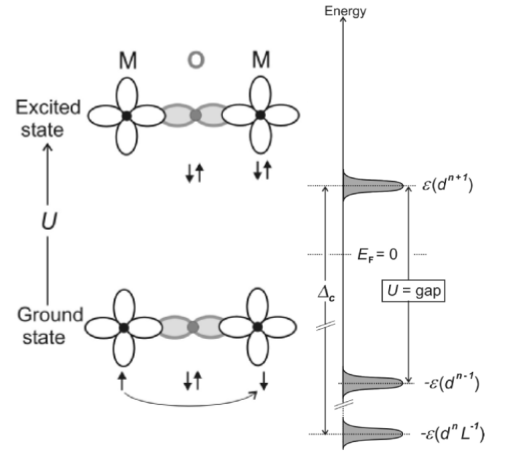
\includegraphics[width=0.5\textwidth]{Mott_mod.PNG}
            \caption{Darstellung des Mott-Hubbard-Isolators. Links im Realraumbild und rechts im Bild der Zustandsdichte.
            Entnommen und modifiziert aus~\cite{stohr_magnetism_2006}.}
            \label{fig:Mott}
        \end{figure}
        \begin{figure}
            \centering
            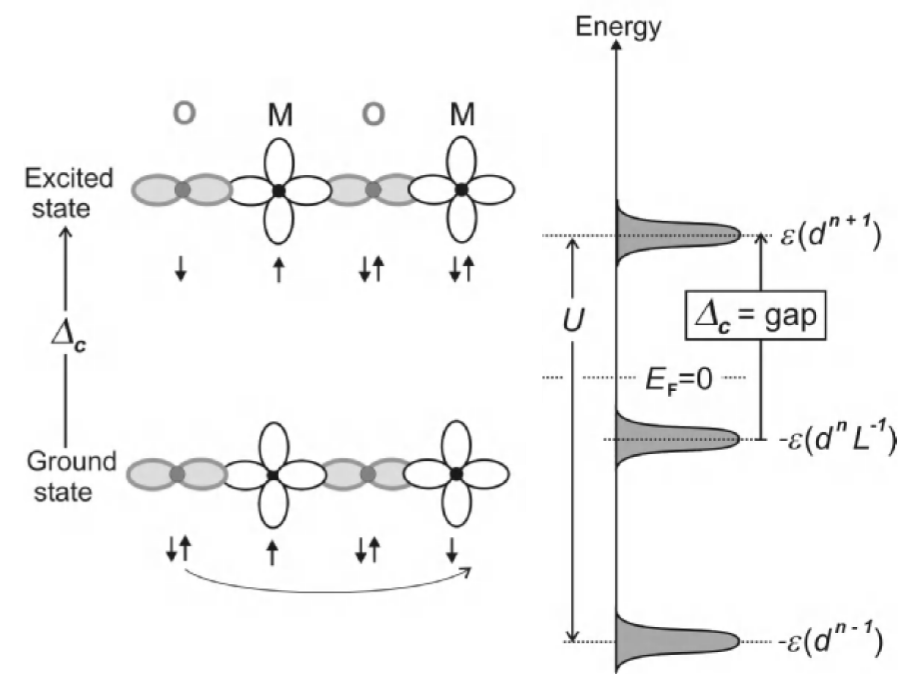
\includegraphics[width=0.5\textwidth]{Charge_mod.PNG}
            \caption{Veranschaulichung der Ladungs-Transferisolator. Links die Veranschaulichungim Realraum und rechts im Raum der Zustandsdichte.
            Entnommen und modifiziert aus~\cite{stohr_magnetism_2006}.}
            \label{fig:Charge}
        \end{figure}
        Die Bandstruktur des Kristalls wird im niederenergetischen Valenzbandbereich durch die überlappenden 2p-Orbitale des Sauerstoffs dominiert.
        Zu höheren Energien hin rührt die Bandstruktur von den überlappenden d-Orbitalen der Übergangsmetalle her.
        Dabei sind die 2p-Zustände stark besetzt wohingegen die d-Zustände nur schwach besetzt sind.
        Bei der Betrachtung der Bandstruktur der Übergangsmetalloxide ist zu beachten, dass diese eine Bandlücke zwischen Valenz- und Leitungsband aufweisen.
        Diese Bandlücke liegt dabei zwischen den besetzen Sauerstoffzuständen und den unbesetzten d-Zuständen des Übergangsmetall.
        Folglich handelt es sich also um Halbleiter oder Isolatoren.
        Durch die Hybridisierung zwischen den p-Orbitalen des Sauerstoffs und den s-Orbital des Übergangsmetall fallen diese als Abschirmung bei den d-Orbitalen weg.
        Beachtung erhalten dann die stark korrelierten und stark delokalierten Elektronen der d-Orbitale~\cite{dane_beschreibung_2008}.
        Ihre entarteten Zustände spalten sich durch die Anwesenheit der Liganden und dessen Kristallfeld auf.
        Bei Monooxiden wird meist eine oktaedrischen Konfiguration des Metallions eingenommen.
        Wodurch die Orbitale $d_{z^2}$ und $d_{x^2-y^2}$ energetisch angehoben und die anderen energetisch abgesenkt werden.
        Vor allem in dem \ce{Fe3O4} in dem das Eisen als (2+) und (3+) Ion auf unterschiedlichen Gitterplätzen (tetraedisch oder oktaedrisch) vorkommt, kommt es zu unterschiedlichen Aufspaltungen der $e_g$ und $t_{2g}$ Energieniveaus.
        
        Es können sich zwei Arte von Bandlücken ausbilden, welche in den Abbildungen \ref{fig:Mott} und \ref{fig:Charge} abgebildet sind.
        Wichtig hierfür ist die Austauschwechselwirkungsenergie $U$, welche die Energie darstellt um ein Elektron von einem Metallatom zu entfernen und es einem weiteren Metallatom hinzuzufügen.
        Auch die Ladungsübertragsenergie~$\Delta$ ist zur Beschreibung notwendig, diese stellt die Energie da um ein Elektron aus dem Liganden zum Metall zu übertragen~\cite{stohr_magnetism_2006}.
        Die erste Art der Bandlücke ist die in der $U$ größer ist als $\Delta$, hierbei handelt es sich dann um Mott-Hubbard-Isolatoren und die Bandlücke wird durch $U$ definiert.
        Im Gegensatz dazu, wenn $\Delta < U$ handelt es sich um so gennate Ladungstransfer-Isolatoren und die Bandlücke wird durch $\Delta$ beschrieben.
        Zu diesen zählt auch das Nickeloxid, dass trotz teilweise gefüllten d-Band ein Isolator ist~\cite{IF_5}.
        
        Die so entstandenen neuen Energieniveaus lassen durch die Wechselwirkung zwischen Ladung, Orbitalen, Gitter und Spin auch magnetische Eigenschaften aufleben.
        So kann durch die Kristallfeldaufspaltung sich \textit{High}- und \textit{Low}-Spin Konfiguration ausbilden.

        Durch die perfekte Anpassung der Austrittsarbeit der Oxide und der damit verbundenen Energieniveauanpassung von aufgebrachten Molekülen lassen sich effiziente organische Halbleiter herstellen.
        Diese erlauben dann einen einfachen Ladungstransfer, da sich die Molekülzuständen nahe der Fermikante befinden~\cite{IF_3}.
        Alleine durch die Veränderung des Oxidationszustands oder Einbringen von Defekten lässt sich dies realisieren, ohne ein neues Material zu nutzen.
        Die untersuchten Übergangsmetalle gehören beide zu den 3d-Übergangsmetallen.
        Im späteren Verlauf wird genauer auf die untersuchten Übergangsmetalloxide eingegangen.

        \begin{itemize}
            \item Oberflächen und Grenzflächen zeigen neue Eigenschaften und Phasen -> Anwendung 
            \item "The interface is the device" von H. Kroemer (Nobelpreis Physik 2000)
            \item Symmetriebrechung, Verspannung (WW mit Substrat), Polarität, Filmdicke, Kristallograpische Orientierung
            \item Die starke Wechselwirkung der e ist die Ursache für die zahlreichen effekte wie Supraleitung und magnetisms in TMO \textbf{Küpper}
            \item Verständnis ist wichtig um Phasenübergänge durch gezielten Doping, Temperatur oder äußeres Magnetfeld für die Anwendung nutzbar zu machen
            \item Magnetische Widerstandsänderung erläutern? (GMR, TMR, CMR)
        \end{itemize}

    
    \section{Antiferromagneten}
        Antiferromagneten (AFM) zeichnen sich dadurch aus, dass Sie nach außen hin kein permanetes magnetisches Moment aufweisen.
        Vereinfacht sind im Inneren die magnetischen Momente vom gleichen Betrag und nebeneinander liegende Momente sind antiparallel untereinander ausgerichtet~\cite{Suter}.
        Dieser Zustand ist allerdings nur unterhalb der Néel-Temperatur $T_\text{N}$ stabil, oberhalb verhälten sich die Antiferromagneten paramagnetisch.
        Die inneren magnetischen Momente richten sich dabei parallel zum äußeren Feld aus und verstärken es somit.
        Um das Phänomen des Antiferromagnetismus zu erklären Bedarf der quantenmechanischen Beschreibung unter Beachtung des Pauli Verbots und der Hundschen Regeln~\cite{TUChemnitz}.
        Es ergibt sich der Austauschwechselwirkungshamiltonien $H_\text{A} = - J_{ik} \vec{S_i}\cdot\vec{S_k}$ der die direkte Wechselwirkung der Spins berücksichtigt.
        Für $J_{ik} < 0$ ergibt sich die antiferromagnetische Kopplung und für $J_{ik} > 0$ eine ferromagnetische Kopplung.
        $J_{ik}$ spiegelt dabei die Stärke der Austauschwechselwirkung wieder und folgt aus dem Überlapp der Wellenfunktionen der beteiligten Elektronen.
        Um eine Aussage über die Ordnung im Antiferromagnet zutreffen gibt es den Ordnungsparameter $L = S^{\uparrow} - S^{\downarrow}$.
        Hierbei ist $S^{\uparrow}$ beziehungsweise $S^{\downarrow}$ der Spin der Untergitter.

        \begin{figure}
            \centering
            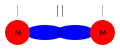
\includegraphics[width=0.6\textwidth]{AFM2.pdf}
            \caption{Darstellung zur Veranschaulichung der antiferromagnetischen Kopplung.
            Als Ligand fungiert hier ein Sauerstoffatom mit seinem p-Orbital (blau).
            Die Spins der d-Orbitale der Metalle (rot) koppeln ferromagnetische mit denen des Sauerstoffs.
            So entsteht die antiferromagnetische Kopplung der beiden Metallatome.}
            \label{fig:AFM}
        \end{figure}
        Ursache des Antiferromagnetismus ist der Superaustausch.
        Beim Superaustausch koppeln zwei Atome mit einem magnetischen Moment über ein weiteres nicht magnetische Atom. 
        Dabei kann die Kopplung ferro- oder antiferromagnetisch sein, meist jedoch antiferromagnetisch~\cite{AFM_1}.
        Sind die beiden koppelnden magnetischen Momente nicht gleich groß, so tritt Ferrimagnetismus auf, es gibt dann eine makroskopische Magnetisierung.
        Der Superaustausch ist winkelabhängig, da es dabei um den Überlapp der Orbitale geht.
        Für die Erklärung wird sich hier nur auf die \SI{180}{\degree} Wechselwirkung beschränkt.
        Beispielhaft ist die Kopplung in \autoref{fig:AFM} dargestellt.
        Es kommt bei diesem indirekten Austausch nicht zu einem Überlapp der spintragenden Wellenfunktionen sondern zu der Vermittlung der langreichweitigen Ordnung über einen Liganden.
        Direkter Austausch sorgt für ferromagnetische Kopplung benachbarter andersartiger (nicht magnetischer) Atome.
        Zwischen Metall und Ligand herscht also direkte Austauschwechselwirkung und damit eine indirekte Austauschwechselwirkung, der Superaustausch zum übernächsten Atom, einem weiteren Metallatom.
        Bei den vorliegenden Metalloxiden ist es so, dass die Elektronen der Metallatom des nicht vollen 3d-Oribtals über die 2p-Orbitale des Sauerstoffs koppeln.
        Da dieses Orbital voll ist, müssen die Elektronen unterschiedliche Spinrichtung haben.
        Damit besitzten die Sauerstoffatome auch kein eigenes magnetisches Moment.
        Somit ist die Wechselwirkung über das Sauerstoffatom hinweg antiferromagnetisch.
        Es ergeben sich zwei Untergitter, welche unterschiedlicher Spinrichtung sind, die Gesamtmagnetisierung ist wie für Antiferromagneten erwartet Null.
        % Die Wellenfunktionen der Kationen überlappen nur gering und da die Austauschwechselwirkung nur geringe Reichweiten hat können nur die 3d und 2p überlappen.
        
        Die Anwendungen des Antiferromagnetismus ist zum Beispiel der Nutzen als \textit{Pinning}-Lage, die in spinelektronischen Bauteilen die Orientierung einer ferromagnetischen Schicht festlegt.
        Eine neue Forschungsidee des europäischen Forschungsprojekt Sinfonia beschäftigt sich mit der Kopplung zwischen Molekülen und Antiferromagneten.
        Ferner sollen diese genutzt werden um Spinwellen, so genannte Magnonen zu generieren und zu detektieren.
        Dies könnte auf Grund der Magnonenfrequenz im \si{\tera\hertz}-Bereich neue Geschwindigkeitsrekorde in der Datenverabeitung bringen~\cite{SINFONIA}.
        
            
    
    \section{Wechselwirkung von Oberfläche mit Molekülen}
        Moleküle haben im Gegensatz zu Festkörpern, energetisch separierte Zustände, die Orbitale.
        Werden Molekül auf eine Oberfläche aufgebracht so kommt es zur Wechselwirkung zwischen diesen und der Struktur der Oberfläche.
        Bei der Wechselwirkung von Molekülen mit Oberflächen wird in zwei Arten der Adsorption unterschieden. 
        Zum Einen in die der Physisorption und zum Anderen in die der Chemisorption, welche wiederum in stark und schwach unterschieden wird.
        Zwischen den beiden Adsorptionsarten lässt sich durch ihre Bindungsstärke zum Substrat hin unterscheiden.
        Dabei wird als Bindungsstärke die Energie bezeichnet, die nötig ist um ein Molekül von der Oberfläche zu lösen.
        In beiden Fällen handelt es sich um eine Adsorption die auch die Oberflächenstruktur des Substrates beeinflussen können.
        So können neue Zustände entstehen und vorhandene Eigenschaften stark verändert werden.
        %~\cite{ma-DJ
        
        \subsection{Physisorption}
            Bei der Physisorption spielt maßgeblich die Van-der-Waals-Kraft eine Rolle.
            Sie hat also eine eher geringe Bindungsenergie der Moleküle zum Substrat~\cite{cinchetti_activating_2017}.
            Da die Wechselwirkung bei der Physisorption nur gering ist werden die Eigenschaften der Oberfläche und des Moleküles nur schwach beeinflusst~\cite{bergenti_spinterface_2019}.
            Die Eigenschaften der Moleküle ähneln also sehr stark den  Eigenschaften aus der Gasphase~\cite{cinchetti_activating_2017}.
            Allerdings kann es beim Substrat zu Relaxation kommen.

            Charakteristisch für die Physisorption ist die Abwesenheit von chemischen Bindungen sowie einen Substrat-Adsorbat-Abstand von mehr als \SI{3}{\angstrom}. %~\cite{bergenti_spinterface_2019}
            Die Van-der-Waals-Kraft gehört zu den elektrostatischen Kräften, es werden also keine Elektronen mit dem Substrat ausgetauscht~\cite{bergenti_spinterface_2019}.
            Allein die Induzierung und Fluktuation von Dipolen führt zu dieser Bindung zwischen Molekül und Substrat.
            Die Van-der-Waals-Kraft kann man in drei Arten unterteilen:
            \begin{itemize}
                \item \textbf{Dipol-Dipol-Kraft:} Sie ist die Kraft zwischen zwei permanenten Dipolen, die Keeson-Wechselwirkung.
                \item \textbf{Dipol-induzierter-Dipol-Kraft:} Die Wechselwirkung zwischen einem induziertem Dipol und einem Dipol wird auch als Debye-Wechselwirkung bezeichnet.
                \item \textbf{Londonsche Dispersions-Wechselwirkung:} Zwischen zwei induzierten Dipolen wirkt die Londonsche Dispersions-Wechselwirkung, sie dominiert meist die Van-der-Waals Kraft.
            \end{itemize}

            Die Physisorption kann durch zwei Potetiale beschrieben werden.
            Das eine Potential wirkt repulsiv und resultiert aus dem Pauliverbot.
            Kommen sich Molekülorbital und Substratorbital zunah, überlappen diese.
            Auf Grund des Pauliverbots dürfen keine zwei Elektronen dann in allen Quantenzahlen übereinstimmen und es resultiert in eine abstoßende Kraft.
            Das zweite und attraktives Potentential resultiert dabei aus der Debye-Wechselwirkung.
            So kommt es beim Gleichgewicht zu einem stabilen Substrat-Molekül-Abstand.
            Das Gesamtpotential ist auch als Lennard-Jones-Potential bekannt.
            Vermehrt tritt die Physisorption bei Halbleitern und Isolatoren auf, da die Molekülzustände in der Bandlücke liegen und so keine Bindung mit dem Substrat eingegangen werden kann~\cite{IF_1}.
        
        \subsection{Chemisorption}
            % Im Gegensatz zur Physisorption findet bei der Chemisorption  ein Austausch von Elektronen stattfinden.
            Im Gegensatz zur Physisorption sind die Bindungen um Einiges stärker und führen somit zu Veränderung am Substrat wie auch den Molekülen~\cite{bergenti_spinterface_2019}.
            Ferner wird von Chemisorption gesprochen, wenn die Stärke der Wechselwirkung größer als \SI{1}{\electronvolt} ist~\cite{muscat_chemisorption_1978}.
            Aber dies allein ist nicht ausschlaggebend, es muss eine chemische Veränderung auftreten.
            Dabei kann es sich um kovalente und ionische Bindungen handeln und es kann zum Ladungsaustausch und/oder Hybridisierung kommen~\cite{harutyunyan_hybridisation_2013}.
            Beim Ladungsaustausch kann ein zunächst unbesetztes Orbital unter die Fermikante rutschen und besetzt werden, es kann also neben den strukturellen auch zu elektronischen Veränderungen kommen.
            Im Gegensatz dazu können bei der Hybridisierung mehrer Zustände vom Molekül und/oder Oberfläche durchmischt werden.
            Verbreiterungen, Verschiebungen und auch Aufspaltungen von Molekülzuständen kann die Folge sein~\cite{IF_1}.

            \begin{figure}
                \centering
                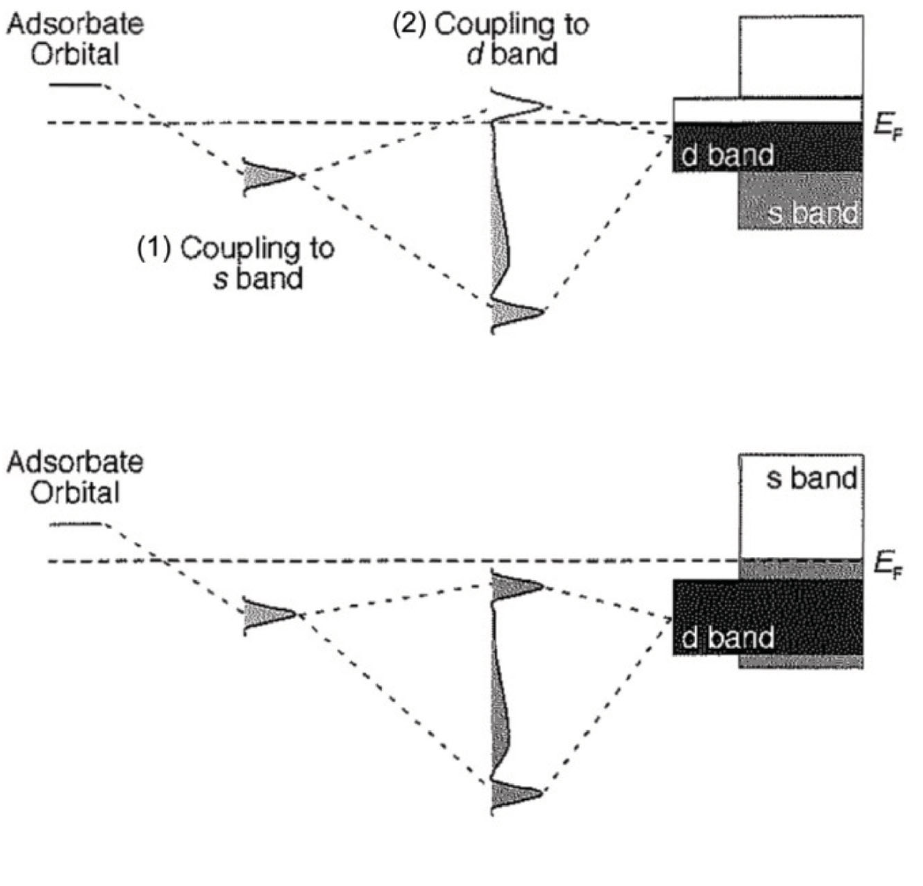
\includegraphics[width=0.5\textwidth]{Chemisorption2.PNG}
                \caption{Das adsorbierte Molekül hybridiziert mit dem s-/p-Band des Substrates (1), der schwachen Chemisorption.
                In einem weiteren Schritt kommt es dann zur starken Chemisorption durch Einbindung der d-Bänder (2, oben), es entsteht ein bindendes und ein antibindenes Orbital.
                Durch die Lage der d-Bänder werden nun das bindenden und antibindendene Orbital besetzt, dadurch kommt es zu einer repulsiven Kraft und die Bindung wird wieder geschwächt (unten). Aus~\cite{IF_1}.}
                \label{fig:Chemisorption}
            \end{figure}
            Schwache Bindungen werden meist durch die Wechselwirkung mit den breiten s- oder p-Bändern hervorgerufen.
            Wodurch sich das Energieniveau der Moleküle absenkt und verbreitert, siehe dazu in \autoref{fig:Chemisorption}.
            Für die starke Chemisorption folgt ein weiterer Schritt, der nun abgesenkte Zustand überlappt mit dem der näherungsweise d-Bänder.
            Es bilden sich bindende und antibindendene Zustände aus.
            Ja nach Lage des Ferminiveaus wird nur der bindende Zustand (starke Adsorption) oder auch (nur teilweise) der antibindende Zustand gefüllt.
            Durch die (teilweise) Füllung des antibindenden Zustands treten repulsiv Kräfte auf und die Adsorptionsstärke wird geschwächt.
            Ferner beeinflusst auch die Ausdehnung der d-Bänder die Stärke der Chemisorption.
        
        \subsection{Selbstanordnung}
            Einige Moleküle ordnen sich regelmäßig auf einem Substrat an, dieser Effekt wird Selbstanordnung genannt.
            Dabei bilden die Moleküle eine Überstruktur im Vergleich zum Gitter des Substrates.
            Gewünscht ist dies, da dann die Molekül einheitlich auf der Oberfläche orientiert sind und somit auch ihre Orbitale, dies ist notwendig für die Molekülorbital-Tomographie (s. \autoref{sec:MOT}).
            Ferner lassen sich gitterartig verteilte Moleküle gezielter manipulieren, wie es für Anwendungen notwendig ist.
            
            \begin{figure}
                \centering
                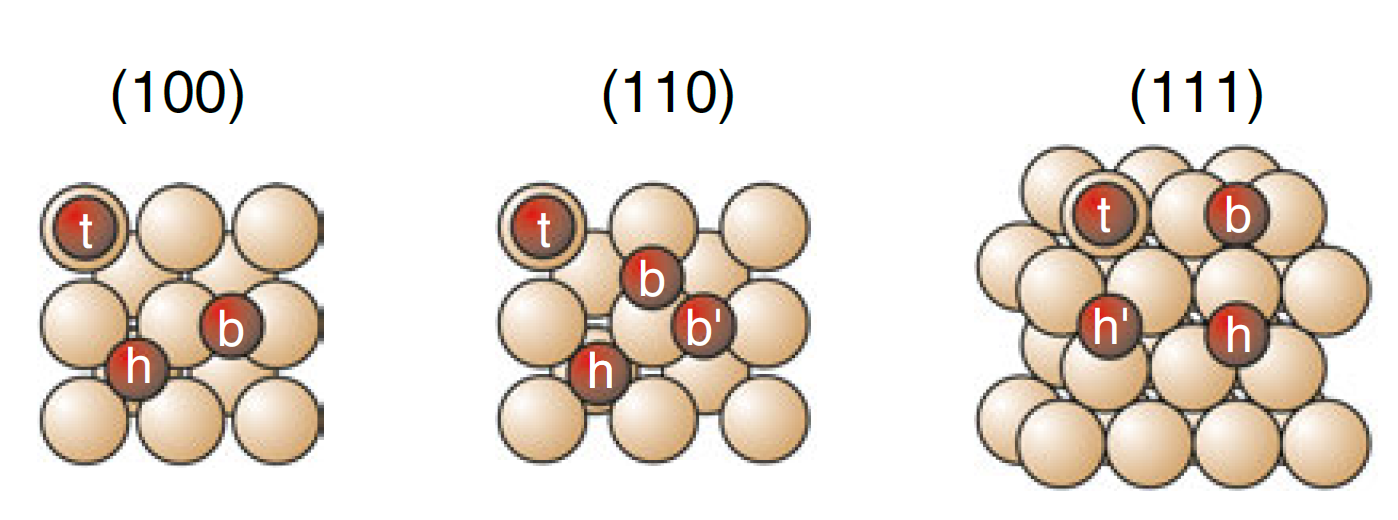
\includegraphics[width=0.6\textwidth]{Adsorbate}
                \caption{Die Adsorbateplätze für verschieden orientierte Oberflächen eines flächenzentrierten Kristalls.
                Es gibt Plätze direkt oberhalb eines Substratatoms (\textit{on top} - t).
                Zwischen zwei Substratatomen gibt es kurze (b) und lange (b') Brückenplätze (\textit{bridge}), sowie Muldenplätze hexagonaler dicht gepacktester Struktur (\textit{hollow} - h) und flächenzentrierter Struktur (h'). Aus~\cite{Fauster}.}
                \label{fig:Adsorbate}
            \end{figure}
            Moleküle stellen eine Art der Adsorbate da und können sich an verschiedene Stellen des Substrates setzen.
            Hier wird auf drei unterschiedeliche Möglichkeiten unterschieden, dem Platz direkt über einem Substratatom (\textit{on top}), zwischen zwei Substratatomen (\textit{bridge}) oder in der Mitte von mehreren Substratatomen in einer Mulde (\textit{hollow}).
            Beispielhaft ist dies für einen flächenzentrierten Kristall mit verschiedenen Oberfläche in \autoref{fig:Adsorbate} dargestellt.
            Die physikalische Ursache ist noch nicht ganz klar, warum sich manche Moleküle auf einigen Substraten ordnen und andere hingegen nicht.
            Naheliegend ist, dass es mit der Wechselwirkung zusammenhängt und der Affinität Elektronen auszutauschen.
            Dies wurde bereits auf die Austrittsarbeit für einige Metaloxide hinweg untersucht~\cite{greiner_universal_2012}.

            Das Wechselspiel zwischen der Molekül-Molekül-Wechselwirkung und Molekül-Substrat-Wechselwirkung definiert die finale Struktur~\cite{IF_1}.
            Dabei sind vor Allem gerichtete Kräfte wichtig um die Regelmäßigkeit zu erhalten.
            Schwächste und ungerichteste Kraft ist die Van-der-Waals-Kraft, genauer die Debye-Wechselwirkung (\SIrange{0.02}{0.1}{\electronvolt}), die allerdings sehr langreichweitig ist.
            Weitere Ursache ist der Einfluss des Substrates auf die Wechselwirkung den Molekülen untereinander, z.B. durch Oszillationen des Oberflächenpotentials.
            Die Keeson-Wechselwirkung als Ursache der Dipol-Dipol-Interaktion hat ebenfalls Beteiligung an der Anordnung der Moleküle, allerdings nur wenn die Moleküle ein permanetes Dipolmoment aufweisen.
            Mit der Wasserstoff-Brücken-Bindung (\SIrange{0.01}{1.73}{\electronvolt}) unter den Molekülen bindet sich ein Wasserstoffatom an ein elektronegativeres Atom, hierdurch kommt es zu Ladungsverschiebung innerhalb der Bindung.
            Das positivere Wasserstoffatom kann nun mehr eine elektrostatische Bindung zu einem weiteren Atom einnehmen.
            Wasserstoff-Brücken-Bindungen sind je stärker sie werden eher geradlinig gerichtete Bindungen mit einer kurzen Bindungslänge.
            Metallisch Koordination ist eine weiter Form der Bindung (\SIrange{0.5}{2}{\electronvolt}), die Moleküle funkieren als Linker zwischen einzelenen Metallatomen.
            Die stärkste und gerichteste Kraft ist jedoch die kovalente Bindung, welche gleichzeitig auch die elektronische Struktur stark beeinflusst.
            Sie ist sogar so stark, dass sie teilweise eine perfekte Selbstanordnung behindert und damit eher zu weniger geordneten Strukturen führen kann~\cite{IF_1}.

            Für die Anwendung besonders wichtig sind wohl geordnete Filme oder kristalline Strukturen.
            Ist die Molekül-Substrat-Wechselwirkung kleiner als die Wechselwirkung zwischen den Molekülen so bilden sich vermehrt geordnete Filme, allerdings sind diese nicht an dem Substrat ausgerichtet.
            Ist im Gegenzug dazu die Wechselwirkung unter den Molekülen geringer als die zum Substrat hin, so bilden sich zunächst Filme aus, welche sich an die Geometrie des Substrates anpassen.
            Mit steigender Schichdicke weicht dies aber immer mehr ab, da dann die Wechselwirkung der Moleküle untereinander überwiegt~\cite{5A_9}.

        \subsection{Energieniveau-Anpassung}
            Für die Anwendung besonders bedeutsam ist die Energieniveau-Anpassung, welche Einfluss auf den Elektronen- und Lochtransport hat~\cite{IF_4}.
            Bei Metalloxiden verschiebt sich durch die Austrittsarbeit $\phi$ die relative Position des Valenz- und Leitungsbandes zum Vakuumniveau~\cite{IF_3}.
            Die meisten der Metalloxide haben keine besetzten Zustände nahe der Fermikante, da diese in eine Bandlücke fällt.
            Folglich ist auch Ladungsübertrag vom Substrat auf die Moleküle nur vom Valenz- oder Leitungsband aus möglich.
            Dies unterscheidet den Prozess maßgeblich von vielen Modellen von Metall-organischen-Grenzflächen.
            Auch wenn einige Oxide Ladungsaustausch zwischen Valenzband und dem höchsten besetzten Molekülorbital (HOMO, \textit{highest occoupied molecular orbital}) zulassen so  gibt es noch kein Model, dass dies beschreibt~\cite{IF_3}.
            Verbreitet ist jedoch der Ansatz der Ferminiveau-Anheftung für nicht reaktive Grenzflächen zwischen Molekülen und Oxiden.

            Greiner u.a.~\cite{IF_3} fanden heraus, dass die Bandstruktur des Substrates dabei nur eine untergeordnete Rolle spielt.
            Ausschlaggebend für die Energieniveau-Anpassung ist das elektrochemische Potential des Substrates mit dem Reduktionspotentials des Moleküls.
            Genauer die Differenz zwischen der Austrittsarbeit des Substrates und der Ionisationsenergie $IE_\text{org}$.
            Als Ionisationsenergie wird die Energie zwischen höchsten besetztem Molekülorbital und dem Vakuumlevel verstanden.
            Die Elektronenaffinität entspricht der Energie zwischen dem Vakuumlevel und dem niedrigsten unbesetzten Molekülorbital (LUMO, \textit{lowest unoccoupied molecular orbital}).
            Als Energie-Offset $\Delta E_\text{H}$ wird der Energiebetrag zwischen HOMO und Fermikante des Substrates verstanden.

            \begin{figure}
                \centering
                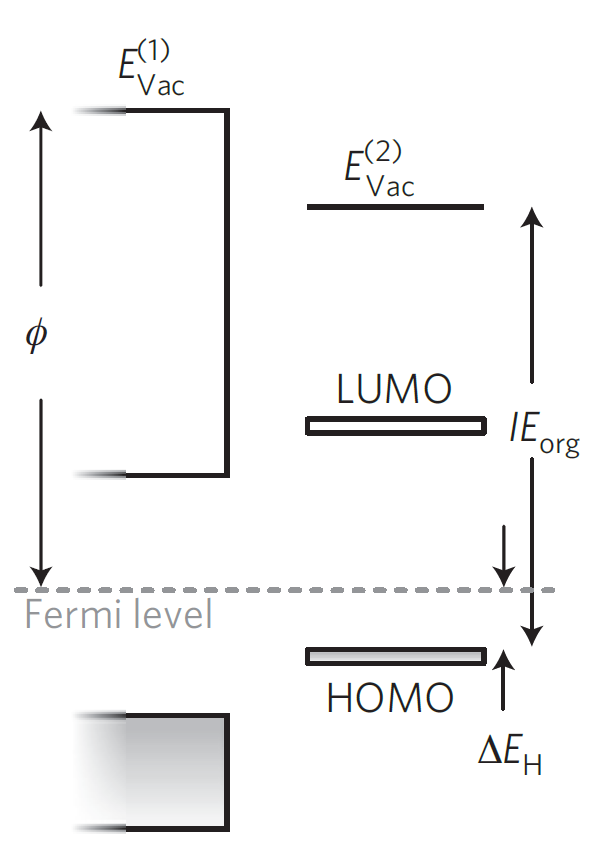
\includegraphics[height=5cm]{E_align.PNG}
                \caption{Veranschaulichung des Energieniveaus für Energieniveauanpassung des Übergangsmetalloxide und Molekülen. Kopiert aus~\cite{IF_3}.}
                \label{fig:E_align}
            \end{figure}
            % \textbf{\cite{IF_3}}
            Ferner gilt das HOMO als des Moleküls Donator-Zustand und das LUMO als Akzeptor-Zustand.
            Bei den Übergangsmetalloxiden gilt das Leitungsband als Akzeptor und das Valenzband als Donator. 
            Nur wenn sich die Donor und Akzeptor der unterschiedlichen Partner stark annähern, kann ein Ladungsaustausch stattfinden.
            Dabei ist zu beachten, dass sich durch die Wechselwirkung die energetisch Lage der Molekülorbital hinsichtlich der Gasphase verschieben können.
            Diese Energieniveaus sind in \autoref{fig:E_align} dargestellt.
            Bei der Verschiebung der Bindungsenergie des HOMOs fällt auf, dass diese sich linear immer weiter einem konstanten Wert annähert, wenn die Differenz zwischen Austrittsarbeit und Ionisationsenergie schrumpft.
            Somit wird das HOMO mit einer gewissen Bindungsenergie an das Fermilevel angeheftet, die nur von der Differenz der Austrittsarbeit und des Ionisationspotential abhängt.
            Der ganze Prozess der Ausrichtung der Molekülzustände an das Ferminiveau des Substrates wird auch Ferminiveau-Anheftung genannt~\cite{IF_3}.

            Weiter gehend ist zu beachten, dass auch bei Isolatoren sich ein Oberflächendipol ausbilden kann.
            Wegen des Pauliverbot und den zusätzlichen Elektronen der Moleküle an der Grenzfläche werden die Elektronen an der Oberfläche in den Festkörper zurück gedrenkt.
            Durch die Unabhängigkeit vom Adsorptionstyp tritt dieser \textit{Push-Back}-Effekt immer auf~\cite{IF_4} und reduziert damit das Oberflächendipolmoment~\cite{IF_1}.
            Zusätzlich kann das Oberflächendipolmoment durch Ladungsaustausch zwischen Molekül und Substrat geschwächt oder andersherum gestärkt werden.
            Hinzukommend gibt es gegebenfalls noch einen permanenten Dipol des Moleküls, welcher beachtet werden muss.
            Diese Effekte beeinflussen die Austrittsarbeit des Materials und somit auch die Ferminiveau-Anheftung.
            Als Folge des Energieniveauanpassung und dem eventuellem Ladungsaustausch oder Hybridisierung kommt es zur Verkürzung der Lebenszeit der Molekülorbital.

    \section{Substrate und Molekül Eigenschaften}
        In diesem Abschnitt geht es um die verschiedenen Substrate die zur Anwendung kommen.
        Des Weiteren geht es ebenso um die verwendeten Moleküle.

        \subsection{Nickeloxid}
            \begin{figure}
                \centering
                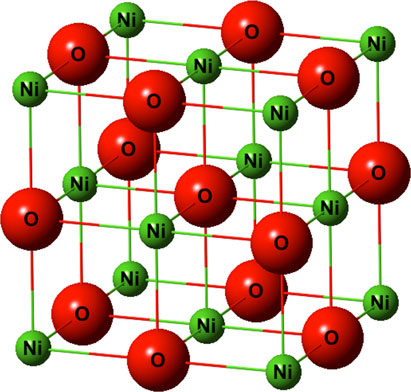
\includegraphics[height=5cm]{NiO/NiO-structure.jpg}
                \caption{Die Krsiatllstruktur von Nickeloxid. Das $\ce{Ni}^{2+}$ Ion befindet sich in einer oktaedrischen Umgebung von $\ce{O}^{2-}$ Ionen. Aus~\cite{NiO-structure}.}
                \label{fig:NiO-structure}
            \end{figure}
            Nickeloxid besitzt die Struktur von \ce{NaCl} und ist in \autoref{fig:NiO-structure} dargestellt~\cite{kunz_chemisorption_1985}.
            Hierbei handelt es sich um ein Monooxid und die Sauerstoffatome sitzen in oktaedrischen Zwischenräumen zwischen den Nickelatomen.
            Die geometrische Gitterkonstante beträgt \SI{4.17}{\angstrom}~\cite{sebbari_uranyl_2012}.
            Für die magnetische Ordnung ergibt sich die dopplte Gitterkonstante zwischen zwei gleich ausgerichteten Spins~\cite{Suter}.
            Die Austrittsarbeit lässt sich dabei durch die Präperation beeinflussen und liegt zwischen \SIrange[range-phrase=\:und\:]{4.5}{5.2}{\electronvolt}~\cite{poulain_electronic_2020}.
            % Neutronenbeugung auf Spin empfindlich also dopplte Einheitszelle, anders als die chemisch empfinliche Röntgenbeugung.

            Nickeloxid gehört zu der Familie der Antiferromagneten mit einer Neél-Temperatur von \SI{525}{\kelvin}.
            Da das 3d-Band des Nickels im Oxid nur teilweise gefüllt ist (acht von zehn möglichen Elektronen) würde erwartet werden, dass es sich hierbei um einen Leiter handelt~\cite{kunz_chemisorption_1985}.
            Dies ist allerdings nicht so und Nickeloxid ist ein Isolator, genauer ein Ladungstransfer-Isolator.
            Die Bandlücke liegt bei \SI{3.6}{\electronvolt}~\cite{kunz_chemisorption_1985}.

            Das Oberflächendipolmoment ist besonders stark in der (111)-Orientierung ausgeprägt, da bei der polaren Oberfläche entweder nur Sauerstoff oder nur Nickelionen in der obersten Lage vorhanden sind~\cite{NiO_8}.
            Dies liegt an der Bindung zwischen dem Sauerstoff und dem Nickel.
            Das Oberflächenpotential ist folglich divergent und somit die Oberfläche instabil.
            Problematisch an dünnen Filmen von Nickeloxid in der (111)-Orientierung ist diese Instabilität und die starke Abhänigkeit vom Präperationsprozess~\cite{NiO_36}.
            Es gibt verschiedene Beobachtungen zu der Stabilisierung der polaren Oberfläche wie die Rekonstruktion oder \ce{OH-}-Terminierung~\cite{NiO_36, NiO_35, NiO_34, NiO_27, NiO_10}.
            Bei der Stabilisierung wird die Oberflächenladung reduziert und damit das Oberflächenpotential gesenkt in Folge dessen es zur Ausbildung einer stabilen Oberfläche kommt.

            Die Magnetisierung ist ebenso wie die Atome abwechseln geschichtet.
            So tritt zunächst eine Ebene mit Nickel auf, in der die Magnetisierung antiparallel zu der nächsten Schicht Nickel ist.
            Die Spins innerhalb einer (111)-Ebene koppeln ferromagnetisch, wohingegen die Kopplung unter den Ebenen antiferromagnetisch ist~\cite{FeO_6}.

            Nickeloxid zeigt bereits für andere Orientierung für einige Moleküle Chemisorption, was durch enthaltene Defekt hervorgerufen wird~\cite{kunz_chemisorption_1985}.
            Auf Grund dessen eignet sich das Substrat zur Untersuchung bestens, zumal für polare Oberflächen auch eine größere Reaktivität vorhergesagt wird~\cite{cappus_hydroxyl_1993}.
            Auch die besondere Orientierung des magnetischen Moments durch die Wahl der (111)-Richtung ist bewusst gewählt, da sich so ein Schichtsystem ergibt bei dem Informationen über Spinwellen nach unten gegeben werden können.
            Besonders die hohe Geschwindigkeit der Magnonen (\si{\tera\hertz}) ist in antiferromagnetischen Materialien zu nutzen~\cite{bossini_macrospin_2016}.
            Hinsichtlich der elektronischen und geometrischen Struktur gibt es bereits zahlreiche Arbeiten~\cite{NiO_7, NiO_34, NiO_35, NiO_37, NiO_8, NiO_13}.
            Ferner besitzt Nickeloxid eine Gitterkonstante die ähnlich zu Gold ist, auf der sich die Moleküle wohldefiniert anordnen~\cite{5A_1}.
            
            Als zukünfiges Material in der Anwendung zeigt Nickeloxid ebenfalls bereits wichtige Eigenschaften.
            So ist Nickeloxid nicht nur ein Antiferromagnet sondern zeichnet sich auch dadurch aus, dass es die Bindungsenergie von adsorbierten Molekülen reduziert.
            Durch die geringe Bindungsenergie des HOMOs eignet sich diese Kombination dabei bestens als Lochinjektion-Material~\cite{IF_3}.
            Damit kann es in organischen Halbleitern und Bauteilen zum Einsatz kommen.

        \subsection{Magnetit}
        \begin{figure}
            \centering
            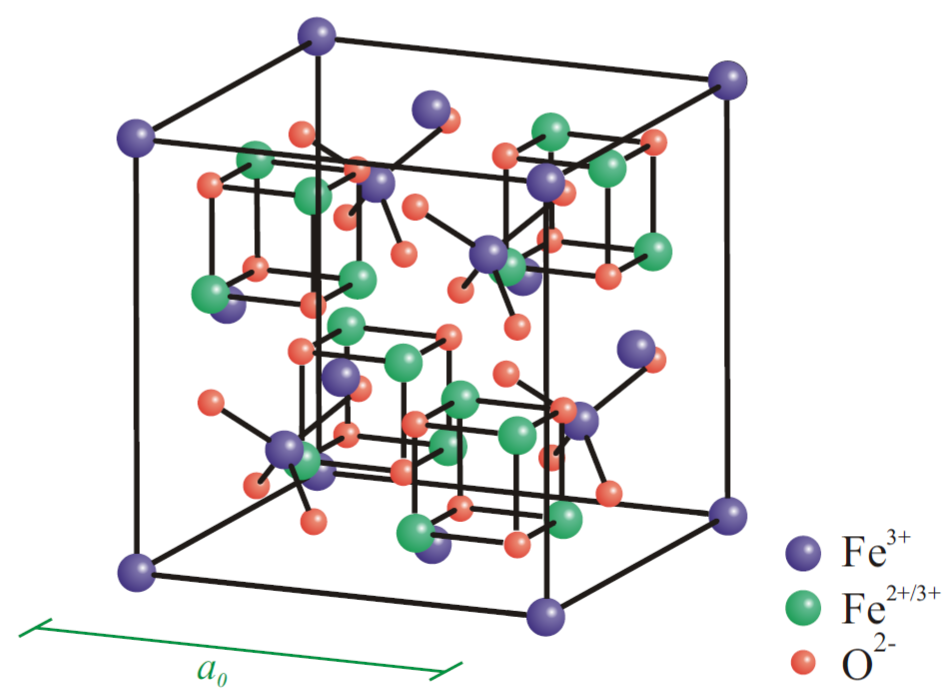
\includegraphics[height=5cm]{Spinell_mod.PNG}
            \caption{Die Krsiatllstruktur von Magnetit. Aus~\cite{bertram_rontgenstrukturanalyse_2009}.}
            \label{fig:Spinell}
        \end{figure}
            Das wohl älteste bekannte magnetische Material ist das Magnetit.
            Die Curie-Temperatur des ferrimagetischen Halbmetall Magentit liegt bei \SI{858}{\kelvin}~\cite{nordmann_anfangsstadium_2014}. % Halbmetall da ein Spinkanal isolierend der ander metallisch
            Chemisch gesehen ist es ein Eisenoxid (\ce{Fe3O4}).
            Magnetit kristallisiert in der in \autoref{fig:Spinell} dargestellten inversen Spinellstruktur, einer kubisch-flächenzentrierten Struktur.
            Die Gitterkonstante beträgt dabei \SI{8.397}{\angstrom}~\cite{springer_database}.
            Zusammen gesetzt ist das Magnetit aus zwei $\ce{Fe}^{3+}$ und einem $\ce{Fe}^{2+}$ zu vier $\ce{O}^{2-}$-Ionen.
            Hierbei befinden sich die $\ce{Fe}^{2+}$-Ionen auf $\sfrac{1}{4}$ der oktaedrischen Lücken.
            Dahingegen sitzen die $\ce{Fe}^{3+}$ zu $\sfrac{1}{4}$ auf oktaedrischen Plätzen und zu $\sfrac{1}{8}$ auf tetraedischen Plätzen.

            Die Bandlücke beträgt bei Raumtemperatur nur etwa \SI{0.1}{\electronvolt}~\cite{FeO_23}, dabei kommt ein ähnliches Prinzip des Ladungstransfer-Isolators zum Einsatz~\cite{FeO_19}.
            Durch den halbmetallischen Charakter weist Magnetit den geringsten elektrischen Widerstand aller Eisenoxide auf~\cite{FeO_23}.
            Interessanterweise unterfährt das Magnetit bei einer Temperatur von \SI{125}{\kelvin} dem Verwey Übergang und wird zum Isolator.
            Dabei ändert es nicht nur seine elektronischen Eigenschaften sondern auch die Geometrischen~\cite{cornell_iron_2003}.

            Die (100) orientierte Oberfläche hat eine $(1\times 1)\text{R}\SI{45}{\degree}$ Oberflächeneinheitszelle mit $\frac{a}{\sqrt{2}}$ Kantenlänge~\cite{bus_studies_2015}.
            Im Gegensatz zu den anderen Eisenoxiden zeigt die Oberfläche eine $(\sqrt{2}\times\sqrt{2})\text{R}\SI{45}{\degree}$ Rekonstruktion gegenüber der (100)-Orientierung des Eisens~\cite{ruwisch_vsm-untersuchung_2016}.
            Die Austrittsarbeit lässt sich dabei auf \SI{5.2}{\electronvolt} bestimmen~\cite{FeO_40}.

            Durch den Ferromagnetismus bei Raumtemperatur  ist das Material besten für die Anwendung geeignet.
            Besonders interessant wird das Material durch die \SI{100}{\percent} Spinpolarisation nahe der Fermikante.
            So lässt sich theoretisch ein unendlich großer magentischer Tunnelwiderstand erzielen~\cite{nordmann_anfangsstadium_2014}.
            Heutzutage wird Magnetit schon in Speichermedien die auf Magnetbändern fundieren eingesetzt, ebenso wie zur Katalyse~\cite{zimmermann_epitaktisches_2010}.


        \subsection{Eisenmonooxid}
            Ebenso wie das Nickeloxid kristallisiert auch das Eisenmonooxid, welches auch Wüstite genannt wird, in der \ce{NaCl}-Struktur~\cite{FeO_4}.
            Dabei beträgt die Gitterkonstante \SI{4.308}{\angstrom}~\cite{springer_database} und die $\ce{Fe}^{2+}$-Ionen befinden sich einer oktaedrischen Position zum Sauerstoff.
            Die $\ce{Fe}^{2+}$-Ionen bezitzen dabei sechs Elektronen im d-Niveau und bilden einen \textit{High}-Spin-Zustand.
            Fünf der sechs Spins sind also parallel ausgerichtet und der verbleibende antiparallel, was den größt möglichen Spin bewirkt~\cite{kupper_electronic_2005}.
            Allerdings ist \ce{FeO} nur oberhalb von \SI{560}{\celsius} stabil.
            Ansonsten handelt es sich um eine nichtstöchiometrische Verbindung.
            So reduziert sich der Anteil an $\ce{Fe}^{2+}$-Ionen und der Anteil an $\ce{Fe}^{3+}$-Ionen steigt~\cite{FeO_11}.
            Es sind also Defekte im Kationenteilgitter und somit wird von $\ce{Fe}_x\ce{O} (x=\num{0.95}-\num{0.88})$ gesprochen~\cite{Chalkogenide}.
            Die Verbindung kann auch in Anteile von Magnetit und Eisen übergehen.
            Dabei verändert sich dann auch die Gitterkonstante, da verschiedene Ionen unterschiedliche Bindungslängen aufweisen.

            Genau wie in Nickeloxid sind auch hier die (111)-Ebenen untereinander antiferromagnetisch gekoppelt.
            Die Neél-Temperatur liegt mit \SI{198}{\kelvin} allerdings unterhalb der Raumtemperatur~\cite{FeO_4}.
            Und die magnetischen Momente der $\ce{Fe}^{2+}$-Ionen sind parallel zu den (111)-Ebenen ausgerichtet.
            So ergibt sich auf der (100)-Oberfläche eine abwechselnde Spinausrichtung.
            Durch die Brechung der Periodizität an der Oberfläche richten sich auch die magnetischen Momente neu aus.
            In der obersten Lage nehmen diese einen Winkel von \SI{25}{\degree} mit der leichten Achse des Kristalls ([111]) hin zur Oberflächennormalen ein.
            Die inneren Lagen zeigen dabei nur noch einen Winkel zwischen \SIrange[range-phrase=\:und\:]{4}{8}{\degree} zur leichten Achse~\cite{FeO_6}.
            Als Defekte wird der Eisenmangel in oktaedrisch Umgebung und die Anreicherung von Eisenionen in tetraedischer Umgebung betrachtet.
            Steigt die Konzentration der Defekte im $\ce{Fe}_x\ce{O}$ an, so steigt ebenfalls die Neél-Temperatur an~\cite{FeO_13}.

            Wie schon das \ce{NiO} ist auch \ce{FeO} ein Ladungstransfer-Isolator mit einer Bandlücke von \SI{2.4}{\electronvolt}~\cite{FeO_21} und einer Austrittsarbeit von \SI{3.5}{\electronvolt}~\cite{FeO_28}.
            Mit dieser Energie ist eine Anregung mittels sichtbaren Lichts möglich.
            Anwendung findet dies zum Beispiel bei nanaokristallienem Eisenmonooxid als Indikator.
            Durch die antiferromagnetische Eigenschaft des Eisenmonooxid ist auch dieses für die Anwendung von optoelektrischen Bauteilen prädestiniert, da die Magnonenfrequenz im \si{\tera\hertz}-Bereich liegt.

            \begin{figure}
                \centering
                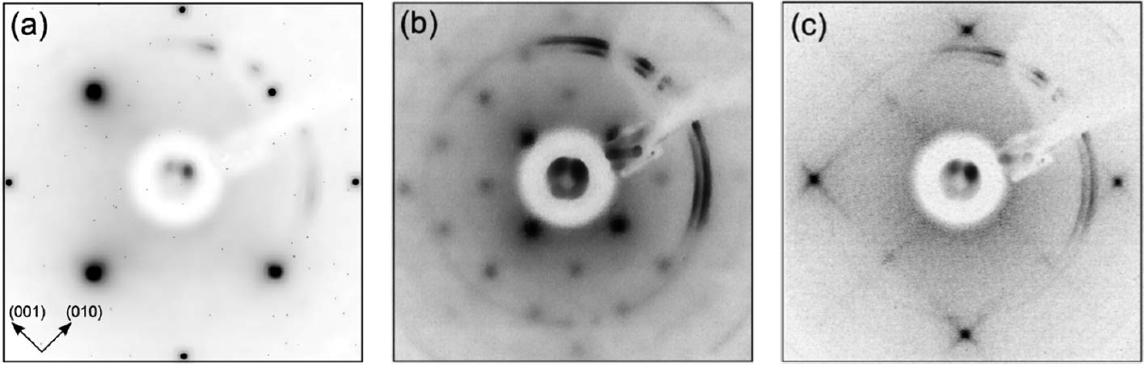
\includegraphics[height=3cm]{LEED_Sub_mod.PNG}
                \caption{Bilder der Beugung niederenergetischer Elektronen der (001)-Orientierung mit einer Elektronenenergie von \SI{125}{\electronvolt}.
                Es sind die Bilder für die passivierte Eisenoberfläche (a), den \ce{Fe3O4}-Film (b) und das Eisenmonooxid (c) gezeigt. Kopiert aus~\cite{FeO_1} und bearbeitet.}
                \label{fig:LEED_Sub}
            \end{figure}
            Die Schwierigkeit bei Eisenmonooxid besteht darin eine wohldefinierte und möglichst defektfrei Oberfläche zu erzeugen.
            Hinsichtlich dessen gab es bereits eine Vielzahl an Studien zu Kristallen des FeOs~\cite{FeO_7, FeO_19, FeO_26, FeO_23, FeO_27}, allerdings nur wenige zu der der Oberflächen~\cite{FeO_1, FeO_4, FeO_29}.
            Entscheidend für die Präperation scheint allerdings das Verhältnis aus Sauerstoffdruck und Aufdampfrate des Eisens zu sein.
            Ebenso wie die zeitliche Abfolge des Aufheizens der Probe sowie Temperaturen.
            Bei der Verwendung von passiviertem Eisen als Substrat lässt sich zunächst ein \ce{Fe3O4} Film erzeugen.
            Entsprechend ergeben sich unterschiedliche LEED-Bilder in \autoref{fig:LEED_Sub}.
            Die \ce{Fe3O4} Oberfläche zeigt dabei ein $\text{p}(2\times 2)$ Überstruktur, da die primitive Einheitszelle der Oberfläche eine Gitterkonstante von \SI{5.9}{\angstrom} besitzt.
            Damit ist sie etwa zweimal so groß wie die des passivierten Eisens mit \SI{2.86}{\angstrom}.
            Anschließend geht der Magnetitfilm in Eisenmonooxid über, wenn die Probe bei \SI{800}{\kelvin} ausgeheizt wird~\cite{FeO_1}.
            Klar ist dies an der Rekonstruktion zu erkennen, welche sich in \autoref{fig:LEED_Sub}(c) ergibt.
            Die Intensität ist dabei invertiert und die Spots sind näher zum Zentrum gerückt, auf Grund der größeren primitiven Oberflächeneinheitszelle mit $a = \SI{3.07}{\angstrom}$~\cite{FeO_1}.
            Die Reinheit kann mittels Augerelektronenspektroskopie \cite{FeO_1} oder eine genauere Identifizierung mit  Röntgenphotoelektronenspektroskopie des \ce{Fe}3p Signals erfolgen.
            Dieser enthält einen Anteil für die $\ce{Fe}^{2+}$ und $\ce{Fe}^{3+}$-Ionen~\cite{FeO_7}.


        \subsection{Pentacene} \label{sec:5A}         
            \begin{figure}
                \centering
                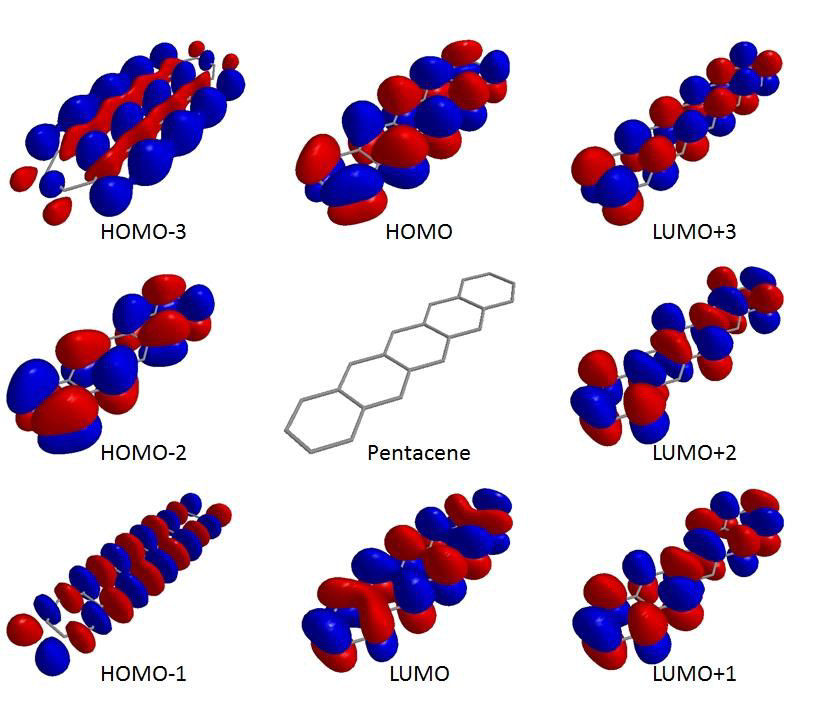
\includegraphics[width=0.6\textwidth]{PEN.jpg}
                \caption{Geometrische Struktur des Pentacene sowei die vier höchsten besetzten und vier niedrigesten unbesetzen Orbitale. Vorlage aus~\cite{PEN}.}
                \label{fig:PEN}
            \end{figure}
            Schon häufig wird Pentacene als kleines Molekül in elektronischen Bauteilen eingesetzt~\cite{5A_4}.
            Bei Pentacene ($\ce{C22H14}$) oder auch kurz 5A handelt es sich um einen Elektronendonator und gehört zu den p-Typ Halbleiter~\cite{5A_1}. % Transport wird maßgeblich durch Löcher verursacht.
            Seine Struktur ist in \autoref{fig:PEN} dargestellt, welche sich aus linear an Kanten verschmolzenen Phenylringen zusammensetzt~\cite{MM_2}.
            Ebenfalls zu sehen sind jeweils die ersten vier höchsten besetzen und niedrigsten unbesetzten Zustände.
            Pentacene bringt die perfekten Eigenschaften für Molekülorbitaltomographie mit, da es sich um ein $\pi$-konjugiertes Molekül handelt~\cite{MM_2}.
            Die Elektronen sind in den $\pi_6$-Orbitalen entlang der Phenylringen starkt delokaliert.
            Dies führt wiederum zu der bisher größten Elektronenbeweglichkeit von \SI{3.0}{\centi\meter\squared\volt\per\second} und ist sogar größer als jene des häufig eingesetzten Silizium mit \SI{1.0}{\centi\meter\squared\volt\per\second}~\cite{5A_13}.
       
            Pentacene zeigte bereits auf zahlreichen Oberflächen reproduzierbares Wachstum von dünnen Filmen bei Raumtemperatur \cite{5A_9}.
            Dabei wurden Metalle wie Gold \cite{5A_6}, Silber \cite{5A_4}, Kupfer \cite{5A_1}, Calcium \cite{5A_5} oder auch dünne Schichten aus Natriumchlorid \cite{5A_10} verwendet.
            Eine bereits häufig verwendete Oberfläche stellt die des Gold (111) dar.
            Auf ihr ordnen sich die Moleküle wohl definiert an und liegen dabei flach und parallel zum Substrat.
            Der Abstand zwischen den Molekülen und Substrat wird auf \SI{3.28}{\angstrom} bestimmt, was in der Größenordnung für Physisorption liegt~\cite{5A_1}.
            Dabei kamen Techniken wie die Rastertunnelmirkroskopie \cite{5A_7}, Beugung niederenergetischer Elektronen \cite{5A_4}, Rötgenphotoelektronenspektroskopie \cite{5A_5} sowie Molekülorbitaltomographie zum Einsatz.
            Die Molekülorbital konnten dabei zuerst mittels Rastertunnelmirkroskopie im Jahre 2011 identifiziert werden~\cite{5A_10}.

            \begin{figure}
                \centering
                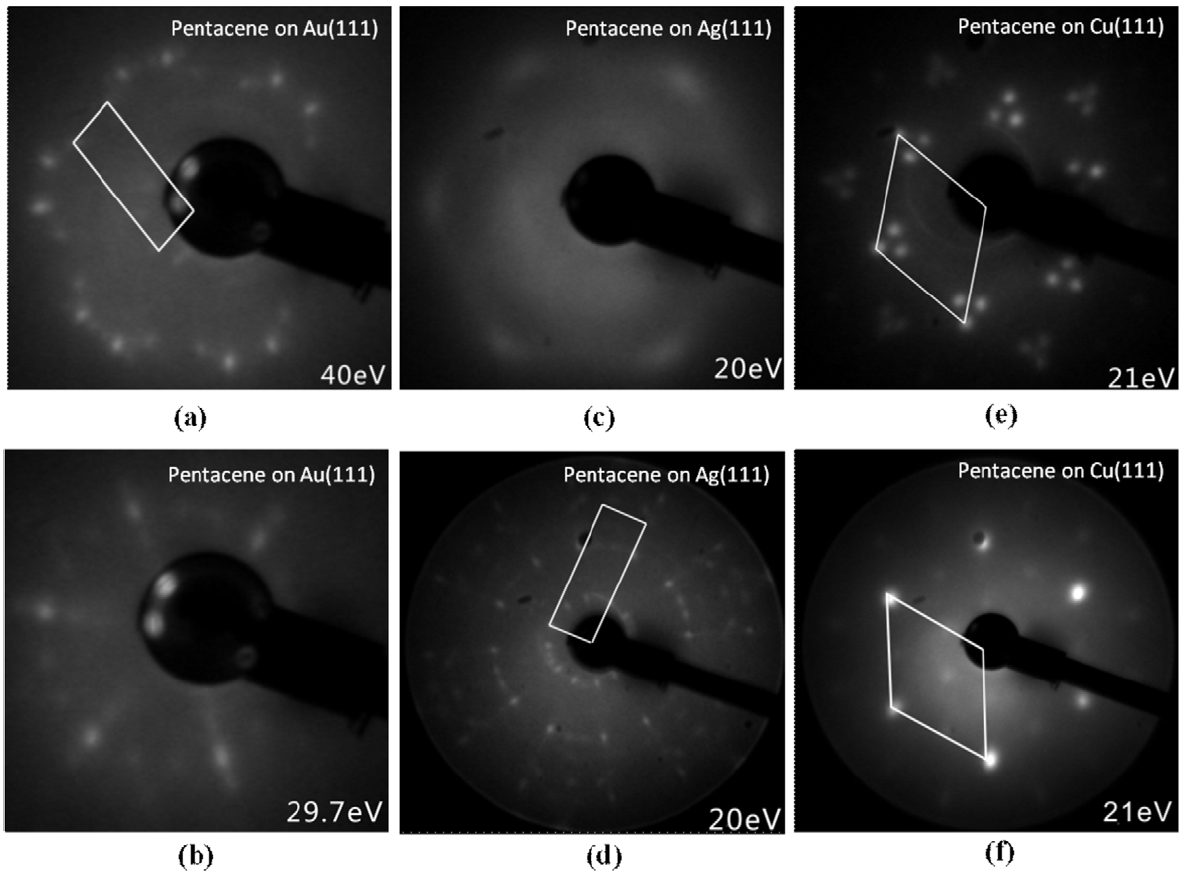
\includegraphics[width=0.6\textwidth]{PEN_Sub.PNG}
                \caption{Bilder der Beugung niederenergetischer Elektronen für verschiedene Schichtdicken und Substrate.
                Die Bilder (a), (c) und (e) entsprechen einer Bedeckung von einer Monolage, die Bilder (b), (d) und (f) einer Bilage Pentacene.
                Kopiert aus~\cite{5A_4}.}
                \label{fig:PEN_Sub}
            \end{figure}
            Dass die Wechselwirkmechanismen zwischen Substrat und Molekül eine entscheidene Rolle darstellen, lässt sich am Beispiel von Gold, Silber und Kupfer zeigen.
            Wie sich in \autoref{fig:PEN_Sub} erkennen lässt ist die Schichtdicke ebenfalls ein wichtiger Faktor bei der Selbstanordnung.
            Für die verschiedenen Substrate und Bedeckungen ergeben sich verschiedene Ordnungen auf der Oberfläche.
            Auch die Wechselwirkung reicht von Physisorption auf Au(111) über schwache Chemisorption auf Ag(111) bis hin zur starken Chemisorption auf Cu(111) \cite{5A_4}.
            Aber auch die Austrittsarbeit der Oberflächen darf bei der Untersuchung nicht ausgeschlossen werden.
            Diese zeigt einen großen Effekt auf die Ausbildung eines Oberflächendipolmoments.
            Je kleiner die Austrittsarbeit wird (je reaktiver das Substrat) desto kleiner wird auch der Oberflächendipol beim Aufbringen auf oragnischem Material \cite{5A_5}. 
            Dabei weist allerdings Pentacene keinen permanenten Dipol auf~\cite{5A_4}.

            Aktuelle Probleme sind allerdings noch die Instabilität unter Atmosphäre sowie die Löslichkeit in verschiedenen Lösungsmitteln, welche zur Massenproduktion unabdingbar ist~\cite{kus_chapter_2018}.
            Allerdings zeigten neuste Studien bereits Erfolge Pentacene aus einer Lösung als dünnen Film aufzubringen~\cite{5A_7}.
            Ein weitere großer Vorteil des Pentacene ist die einfache Herstellung \cite{kus_chapter_2018} und die Zusammensetzung aus leichten Atomen.
            Mit einer Dichte von nur \SI{1.232(6)}{\gram\per\cubic\centi\meter} ist es besonders leicht, was einen Vorteil für die mobile Anwendungen mit sich bringt~\cite{CAS}.
            
            In einigen Bauteilen kommen die Moleküle auch heutzutage schon als organischer Halbleiter zum Einsatz.
            Ausgezeichnet sind sie dafür durch die hohen Elektronenmobilität und der geringen Größe.
            Zum Bespiel in Transistoren \textbf{Lin et al. - 1997 - Pentacene-based organic thin-film transistors.pdf} und Luftfeuchtigkeitssensoren \cite{demelas_chemical_2015} werden diese heute schon verwendet.
            Eine Verwendung in Solarzellen ist ebenfalls denkbar \cite{shirota_1_2019}.
            Auf Grund dessen ist eine weitere Erforschung interessant.
            So werden für den Einsatz in oragnischen Feldeffekt-Transistoren eine Schicht aus isolierendem Material, wie zum Beispiel \ce{NiO} oder \ce{FeO} und Molekülen, wie dem Pentacene benötigt~\cite{5A_13}.
            Diese Bauteile können dann in bestehende Schaltungen eingebaut werden und erhöhen so die Effizienz und können dabei die Baugröße reduzieren, sowie zur Reduktion des Gewichts beitragen.
            Versuche zur Anordnung von Pentacene auf den \ce{NiO}(111) und \ce{FeO}(100) Oberflächen konnten aktuell noch nicht beobachtet werden.
            Wohl ist aber bekannt, dass sich Pentacene auf $\ce{Fe}-\text{p}(1 \times 1)\ce{O}$ strukturiert anordnet.
        

            \section{IDEEN}
            \begin{itemize}
                \item O1s erklären
                \item Fe3p erklären 
                \item XMLD
                \item XPS ausführlicher? (Asymmetrie)
                \item mehr Motivierend aktuelle Anwendung
            \end{itemize}
            
\chapter{Methoden und Techniken} \label{cha:Methoden}
    In diesem Kapitel geht es um die grundlegenden Bedingungen zur Untersuchung von Molekülen auf antiferromagnnetischen Oberflächen.
    Dazu gehört zunächst das Ultrahochvakuum, welches notwendig ist um eine saubere und wohl definierte Oberfläche zu erhalten.
    Ferner wird die Methode Beugung niederenergetischer Elektronen erläutert, womit auf die geometrische Struktur der Oberfläche geschlossen werden kann.
    Anschließend geht es um die Photoelektronenspektroskopie und ihre Teilbereiche, welche eine Untersuchung der elektronischen Struktur zulässt.

    \section{Grundlegende Bedingungen} \label{sec:Grundlagen}
        Um sich Oberflächen genauer anzusehen muss zunächst verhindert werden, dass sich keine unerwünschten Teilchen auf der Oberfläche absetzen.
        Hierzu wird Ultrahochvakuum (UHV) eingesetzt.
        Da es keine Pumpe gibt, die direkt vom Atmosphärendruck bis in den UHV Bereichen kleiner \SI{1e-9}{\milli\bar} reicht, ist ein mehrstufiges Pumpsystem unabdingbar \cite{Henzler}.
        In dem vorliegenden Aufbau wird dies durch Turbomolekularpumpen mit vorgeschalteten Scrollpumpen realisert.
        Ferner werden diese durch Titansublimationspumpen, sowie Ionenpumpen unterstützt.
        Diese tiefen Drücke sind erforderlich, da schon bei einem Druck von \SI{1e-6}{\milli\bar} die Oberfläche innerhalb von \SI{10}{\milli\second} zu \SI{1}{\percent} mit den im Restgas vorhandenen Teilchen bedeckt wäre~\cite{Henzler}.

        Es gibt auch die Möglichkeit gezielt Gase in die Präperationskammer zu leiten, in der die Proben für die anschließenden Messungen vorbereitet werden.
        Dies geschieht dann durch sogenannte Leckventiele.
        Ein Maß für die Oberflächenbedeckung ist die Einheit Langmuir \si{\langmuir}, welcher einer Dosis entspricht.
        Dabei ist $\SI{1}{\langmuir} = \SI{1}{\torr} \cdot \si{\micro\second}$ also etwa $\SI{1.33e-6}{\milli\bar} \cdot \si{\second}$.
        Hier wird zu Grunde gelegt, dass jedes auf die Oberfläche auftreffende Teilchen auch haften bleibt. 
        Die Oberfläche besäße also einen Haftkoeffizienten von Eins, was in der Realität so nicht vorkommt.

        Das Vakuum dient allerdings nicht nur der Reinheit der Probe, sondern auch das die später emittierten Elektronen den Raum durchdringen und den Analysator erreichen können.
        Andernfalls würden die Elektronen durch Streuung an anderen Teilchen abgebremst werden und somit ihre Informationen verlieren.
        % Elektronen hätten bei einem Druck von xx bar nur eine Reichweite von \textbf{QUELLE, Zahlen}.
        Da es sich um die Untersuchung von Oberflächen handelt ist somit auch bei den Techniken auf die Oberflächensensitivität zu achten.
        Relevant wird damit die mittlere freie Weglänge der verwendeten Sonde.
        Als perfekte Sonden stellten sich die Elektronen heraus, ihre inelastische mittlere freie Weglänge ist in \autoref{fig:Weg} graphisch dargestellt.
        \begin{figure}
            \centering
            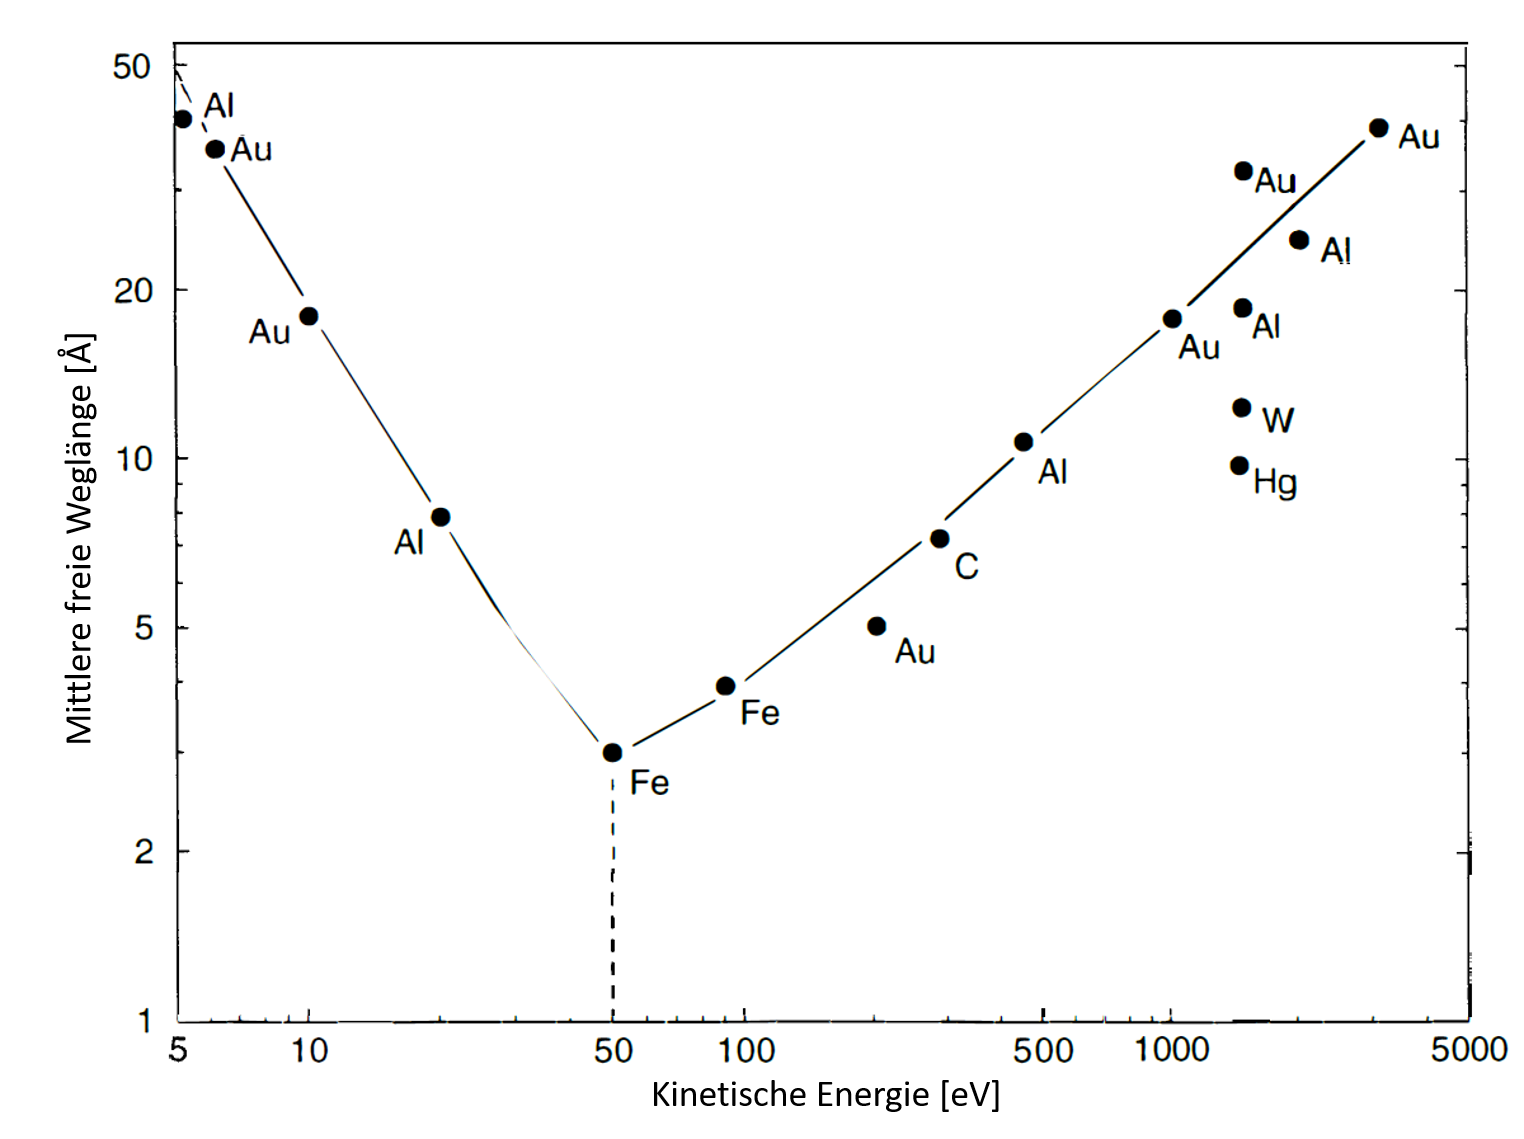
\includegraphics[width=0.7\textwidth]{Weg}
            \caption{Die mittlere freie Weglänge für Elektronen in verschiedenen Materialien. Aus~\cite{Hüfner}.}
            \label{fig:Weg}
        \end{figure}
        Es ist zu erkennen, dass Elektronen mit einer kinetischen Energie im Bereich von \SIrange{30}{100}{\electronvolt} aus einer Tiefe von nicht mehr als \SI{5}{\angstrom} kommen.
        Werden also Elektronen als Sonden verwendet und ihre kinetische Energie angepasst, so kann davon ausgegagngen werden, dass sie nur aus oberflächennahen Bereichen kommen.

        Um Elektronen von der Probe kommend zu erhalten gibt es zwei Möglichkeiten.
        Zünächst können Elektronen in der Probe angeregt werden, die dann aus der Oberfläche austreten und detektiert werden.
        Dies wird bei der Photoelektronenspektroskopie genutzt und in \autoref{sec:PES} genauer erläutert.
        Die zweite Möglichkeit ist es die Probe mit Elektronen im entsprechenden Energiebereich zu beschießen.
        Zurückkommenden Elektronen mit identischer kinetischen Energie können also nur aus oberflächennahen Bereichen kommen.
        Bei der Beugung niederenergetischer Elektronen wird dieses Prinzip verwendet und nun genauer beschrieben.

    \section{Beugung niederenergetischer Elektronen} \label{sec:LEED}
        \begin{figure}
            \centering
            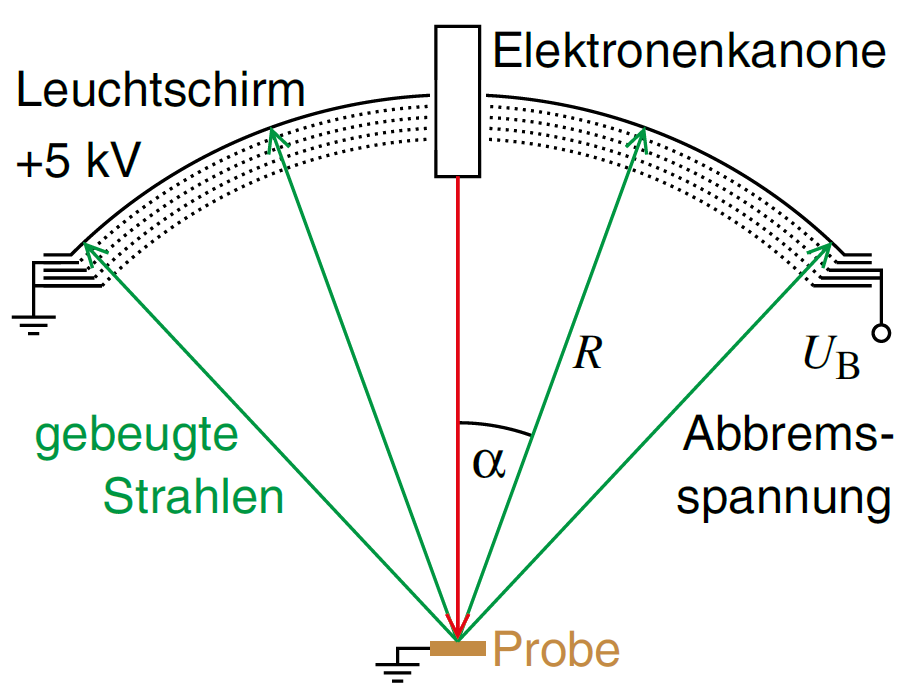
\includegraphics[width=0.5\textwidth]{LEED}
            \caption{Innerer Aufbau der Optiken zur Beugung niederenergetischer Elektronen.
            Die Probe befindet sich im Zentrum des Schirms und auf Erdpotential, ebenso wie das erste und dritte Gitter.
            Die Abremsspannung liegt am zweiten Gitter an, am vierten Gitter die Beschleunigungsspannung.
            Aus~\cite{Fauster}.}
            \label{fig:LEED}
        \end{figure}
        Um sich die geometrische Oberflächenbeschaffenheit genau anzusehen wir die Beugung niederenergetischer Elektronen (\textit{Low energy electron diffraction}, LEED) eingesetzt.
        Hierbei werden Elektronen mit einer kinetischen Energie im Bereich der Oberflächensensitivität auf die Probe geschossen.
        Das entstehende Beugungsmuster ist charakteristisch für die Oberflächenbeschaffenheit und stellt die Oberfläche im reziproken Raum da.
        Der Aufbau mit seinen Optiken für die Beugung niederenergetischer Elektronen ist in \autoref{fig:LEED} abgebildet.
        
        Die Elektronen werden zunächst durch den Glühelektrischen Effekt erzeugt und durch einen Wehnelt-Zylinder gebündet.
        Diese beiden Komponenten bilden zusammen die Elektronenkanone.
        Anschließend werden Sie zur Probe hin beschleunigt, welche sich im Zentrum der Gitter befindet.
        Da die Probe geerdet ist geschieht dies durch eine negative Vorspannung zwischen Probe und Elektronenkanone.
        Die gestreuten Elektronen bewegen sich in alle Richtungen unter dem Winkel $\alpha$ zum senkrecht auftreffenden Elektronenstrahl von der Probe weg.
        Damit die Flugbahn nicht durch elektrische Felder beeinflusst wird befindet sich das erste von der Probe aus gesehen Netz ebenfalls auf Erdpotential.
        Genau der Vorspannung entsprechend wird durch das dahinter liegende Netz  ein elektrisches Feld aufgebaut, gegen das die Elektronen anlaufen.
        So können nur elastisch gestreute Elektronen die weiteren Netze durchlaufen.
        Das nächste Gitter liegt wieder auf Erdpotential, damit das vom dahinter liegenden Gitter erzeugte Beschleunigungsfeld nicht durchgreift.
        Dieses Beschleunigungsfeld wir durch eine hohe Spannung hervorgerufen und ist dafür notwendig, damit die Elektronen auf dem Leuchtschirm das Beugungsmuster erzeugen können.
        Mit Hilfe einer Kamera wird dieses Beugungsmuster erfasst ~\cite{Fauster}.

        Die Entstehung des Beugungsmusters geschieht durch Interferenz Effekte, es ist also eine periodische Struktur von Nöten.
        Ebenso muss damit die Wellenlänge der Elektronen im Größenbereich der Gitterkonstanten liegen.
        Folglich haben die Elektronen einer Energie zwischen \SIrange{30}{200}{\electronvolt}~\cite{oura_surface_2003}.
        Kinematisch betrachtet wird die Oberfläche von einer Primärwelle getroffen.
        Der von einem Streuer zurückgeworfene Anteil (ohne zusätzliche Streuung) interferiert mit den von anderen Streuen kommenden Sekundärwelle.
        Für elastisch gestreute Elektronen muss also für den Impuls gelten $\abs*{\vec{k}_\text{i}} = \abs*{\vec{k}_\text{f}}$.
        Intensitäten der einzelnen Spots $I$ ergeben sich dabei aus dem Formfaktor $F$ und dem Gitterfaktor $G$ zu
        \begin{equation}
            I = \abs*{F^2}\abs*{G^2}.
            \label{eqn:LEED}
        \end{equation}
        Mathematisch kommt der Formfaktor aus der Position und chemischen Natur der Atome innerhalb der Einheitszelle, wohingegen der Gitterfaktor die Periodizität der Gitters wiederspiegelt.
        Der Gitterfaktor ist nur ungleich Null, wenn die Lauebedingung erfüllt ist.
        Folglich darf der Impulsübertrag $\increment \vec{k}_{||}$ nur einen reziproken Gittervektor $\vec{g}_\text{hk}$ betragen, dies ist die Lauebedingung.
        Jeder Spot kann damit einem Impulsübertrag mit den Indizes $hk$ zugeordnet werden.
        Der Gitterfaktor gibt also nur Auskunft darüber ob ein Beugungsreflex auftaucht und wo, die Intensitäten hingegen werden rein durch den Formfaktor beschrieben.

        Da aber wie oben beschrieben die Impulserhaltung gelten muss und die Transaltionssymetrie senkrecht zur Oberfläche gebrochen ist ergibt sich für diese Komponente ein Impuls von $\vec{k}_{\text{f}\perp} = \pm \sqrt{\vec{k}_\text{i}^2 - (\vec{k}_{\text{i}||} + \vec{g}_\text{hk})^2}$.
        Positives Vorzeichen entspricht der Beugung in die Oberfläche hinein und negatives Vorzeichen für eine Beugung von der Oberfläche weg.
        $\vec{k}_{\text{f}\perp}$ kann auch imaginär werden, was zur Folge hat, dass keine Rückstreuung erfolgt.
        \begin{figure}
            \centering
            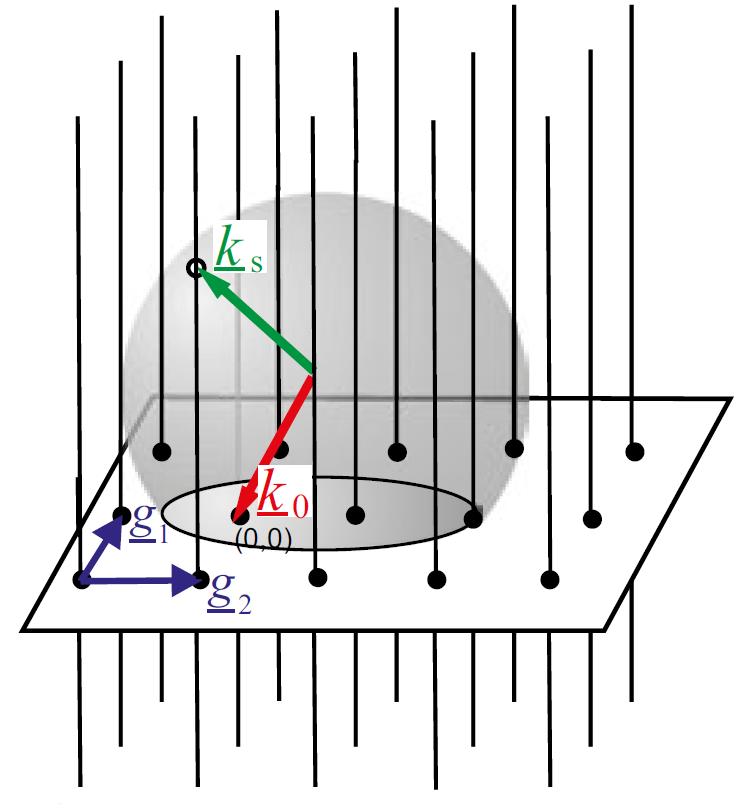
\includegraphics[width=0.4\textwidth]{Ewald}
            \caption{Schamtische darstellung zur Veranschaulichung der Konstruktion der Ewaldkugel.
            Blaue Pfeile stellen die reziproken Gittervektoren da. 
            Der rote Pfeil den einfallenden Wellenvektor der Elektronen, grün den der gestreuten.
            Kopiert und modifiziert aus~\cite{Fauster}.}
            \label{fig:Ewald}
        \end{figure}
        Die Beugungsreflexe lassen sich für nahezu senkrechten Einfall mit Hilfe der Ewaldkugel konstruieren, veranschaulicht zu sehen in \autoref{fig:Ewald}.
        Hierzu wird das reziproke Gitter aufgespannt, es ergeben sich auf Grund der gebrochenen Symmetrie Gitterstangen.
        Um einen beliebiegen Startpunkt wird eine Kugel mit dem Radius $\vec{k}_\text{i}$ gezeichnet, so ergeben sich für alle schneidenen Gitterstangen der Kugel auch Beugungsreflexe.
        Der Schnittpunkt mit der Kugel zum Ursprung hin ergibt dann den gebeugten Wellenzahlvektor $\vec{k}_\text{f}$.

        % Größere Abstände im Realraum werden im reziproken Raum kleiner abgebildet.
        % Mit steigeneder Energie der Elektronen rücken die Beugungsmaxima dichter zum Zentrum hin.
        Die Annahme ohne Mehrfachstreuung der Elektronen ist zu einfach gefasst, weswegen lange keine Strukturanalyse mittels LEED möglich war.
        Ursache der Mehrfachstreuung ist der verhältnissmäßig große Streuquerschnitt der langsamen Elektronen an Atomen.
        Es kommt vermehrt zur Streuung mit den nächsten Nachbarn der Primär- wie auch Sekundärwelle, die sich wiederum gegenseitig beeinflussen.
        Tendenziell ist es möglich aus der Position der Beugungsreflexe auf die Größe der Einheitszelle zu schließen, durch Adsorbate und Domänen, kann dies allerdings erschwert werden.
        Werden die Intensitäten der Spots durch Variation der Energie aufgezeichnet ergeben sich charakteristische IV-Kurven.
        Ihre theoretische Berechnung ist sehr aufwendig, da sie den Formfaktor und zahlreiche Streueffekte berücksichtigen müssen.

    
    \section{Photoelektronenspektroskopie} \label{sec:PES}
        Die Grundlage ist der Photoelektronenspektroskopie ist der photoelektrische Effekt, der 1905 zum ersten Mal von Albert Einstein erklärt wurde~\cite{Einstein}.
        Hierbei werden Elektronen durch ein einfallendes Photon angeregt.
        Ist die Energie hoch genug, so treten diese aus der Probenoberfläche aus.
        In Formeln ergibt sich so die kinetische Energie der Elektronen, die die Probe verlassen zu 
        \begin{equation}
            E_{\text{Kin}} = h \nu - E_{\symup{B}} - \phi
            \label{eqn:Photoeffekt}
        \end{equation}
        mit der Bindungsenergie des Elektrons $E_{\symup{B}}$, der Energie des einfallenden Photons $h \nu$ und der Austrittsarbeit $\phi$.
        Die Austrittsarbeit ist der Energieunterschied zwischen der Fermienergie $E_\text{F}$ und der Vakuumenergie $E_\text{V}$.
        Erkennbar ist also, dass sich die kinetische Energie immer auf die Vakuumenergie bezieht wohin gegen die Bindungsenergie sich auf die Fermienergie bezieht und für gebundene Zustände stets positiv dargestellt wird.
        
        \begin{figure}
            \centering
            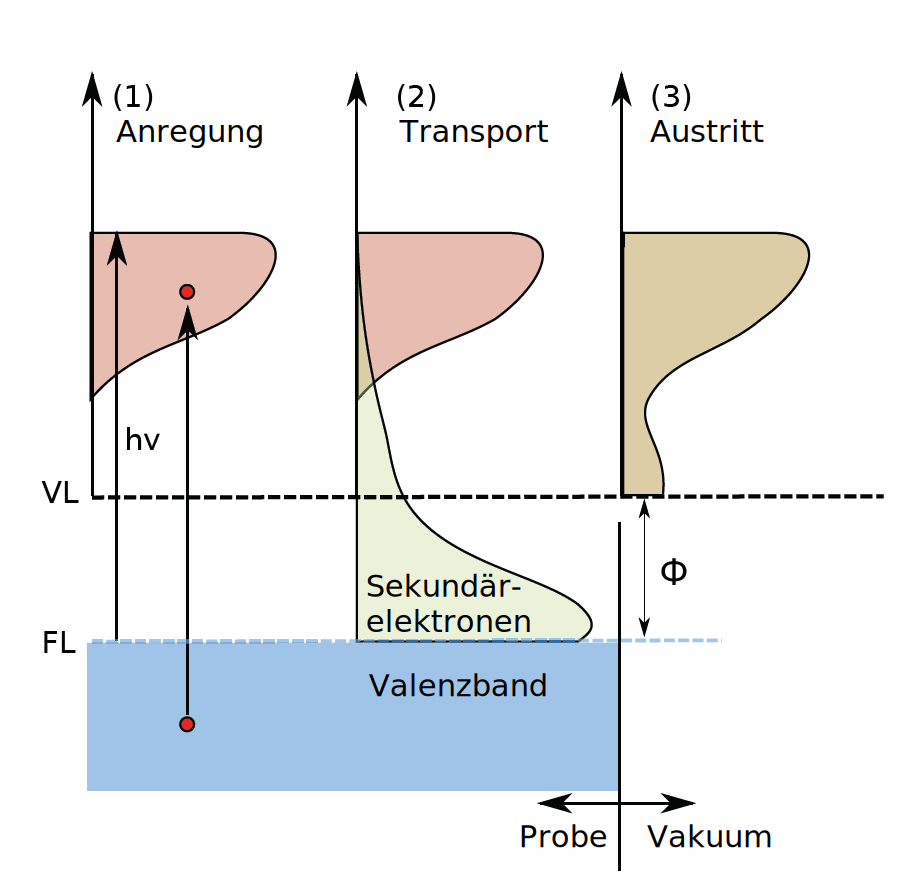
\includegraphics[width=0.6\textwidth]{3Stufen}
            \caption{Schematische Darstellung des drei Stufen Models für den photoelektrischen Effekt.
            Bestehend aus (1) Absorption, (2) Transport zur Oberfläche und (3) Austritt aus der Oberfläche.
            Kopiert und modifiziert aus~\cite{zhang_synchrotron_2018}.}
            \label{fig:3Stufen}
        \end{figure}
        Dieser Prozess der Emittation eines Elektrons nach Einfall eines Photons lässt sich in einem drei Stufen Model erklären.
        Das Model ist in \autoref{fig:3Stufen} schematisch zu sehen.
        Der erste Schritt ist die Absorption des Photons, wodurch das Elektron angeregt wird. 
        Dieses kann dann innerhalb des Festkörpers zur Probenoberfläche wandern.
        In diesem zweiten Schritt kommt auch die mittlere freie Weglänge der Elektroen zu tragen, weshalb die Methode oberflächensensitiv ist.
        Im dritten Schritt verlässt das Elektron die Oberfläche und wird auf Grund fehlender periodischer Strukturen gebeugt.
        Hier ist die Periodizität des Festkörpers gebrochen, wodurch die senkrechte Komponente des Impulsvektors nicht erhalten bleibt.
        Dahingegen bleibt der Impulsvektor parallel zur Oberfläche $k_{||}$ erhalten.

        \begin{figure}
            \centering
            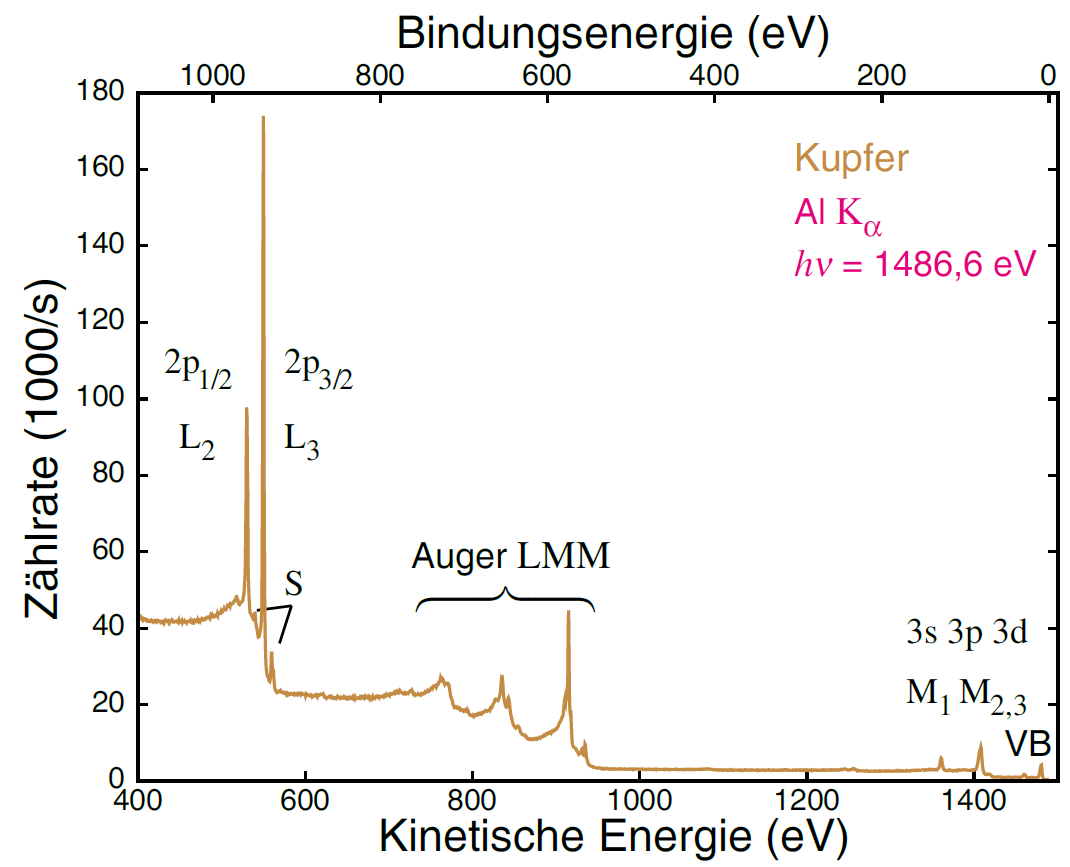
\includegraphics[width=0.6\textwidth]{Band}
            \caption{Ein Photoemissionsspektrum von Kupfer.
            Im niedrigen Bindungsenergiebereich befindet sich das Valenzband. 
            Zu höheren Bindungsenergien treten dann die Kernniveaus in den Vordergrund, gemeinsam mit den Augerelektronen-Peaks und satelliten-Linien.
            Aus~\cite{Fauster}.}
            \label{fig:Band}
        \end{figure}
        Ein beispielhaftes Spektrum ist in \autoref{fig:Band} zu finden.
        Die Fermikante, bis wohin alle Zustände besetzt sind ist im Spektrum nicht zu erkennen, legt allerdings die Bindungsenergie \SI{0}{\electronvolt} fest.
        Im niederenergetischen Bindungsenergiebereich handelt es sich um Zustände des Valenzbandes zu höheren Energien treten Zustände der Kernniveaus auf.
        Zusätzlich treten diskrete Linien auf, die durch Augerelektronen hervorgerufen werden.
        Diese Augerelektronen besitzen immer eine feste kinetische Energie, da sie durch den Übergang zwischen zwei Schalen stammen und somit unabhängig von der verwendeten Photonenenergie.
        Zum Ende des Spektrums nimmt der Untergrund stetig zu, was durch inelastisch gestreute Elektronen zustande kommt.
        Nach jedem Peak steigt der Untergrund stufenartig an, da vermehrt Elektronen für die Streuung bereitstehen.
        Im Bereich der niedrigen kinetischen Energie nimmt dieser Effekt ein Maximum an, die Sekundärelektronen.
        Zusätzlich im Spektrum sind Satelieten (S) zu sehen, diese stammen von der nicht ganz monochromatischen Photonenstrahlung. %Übergang von Elektronen bei mehrfachionisierten Atomen.

        Je nach Energie der verwendeten Photonen lässt sich in maßgeblich zwei Bereiche unterscheiden.
        Zum Einen in den Bereich der Röntgenstrahlung (\textit{X-Ray}), womit kernnahe Zustände untersucht werden.
        Zum Anderen den Bereich der ultravioletten Strahlung, hier können Zustände nahe der Fermikante sichtbar gemacht werden.
        Die verschiedenen Energiebereich sind notwendig, damit die angeregten Elektronen eine kinetische Energie im oberflächensensitiven Bereich haben.
        Diese erste Methode wird XPS genannt, wohingegen die zweite Methode mit UPS abgekürzt wird.

        \subsection{Röntgenphotoelektronenspektroskopie - XPS}
            In den Energiebereich der weichen Röntgenstrahlung fallen Photonen mit einer Energie von \SIrange{0.1}{10}{\kilo\electronvolt}~\cite{Fauster}.
            Diese Energien sind nur mit klassischen Röntgenquellen oder einem Synchrotron erreichbar.
            Solche hohen Energien sind notwendig um Elektronen aus Kernniveaus anzuregen.
            % Die kernnahen Niveaus sind schwieriger zu beeinflussen und eigenen sich besonders gut zur Elementanalyse.
            Mit dieser Methode lässt sich ebenfalls die chemische Zusammensetzung untersuchen.
            Leicht unterschiedliche Positionen für verschiedene Ionisationszustände und Bindungszuständen können dabei Rückschlüsse auf chemische Umgebungen zulassen.
            So verschiebt sich die Energie auch, je nach dem ob die Atome an der Oberfläche oder tiefer im Festkörper sind von denen die Elektronen emittiert werden.

            Ein einzelnes so detektierte Merkmal unterliegt dabei mehrern Effekten. 
            Die Breite des charakteristischen Merkmals wird durch die Energiebreite der verwendeten Photonen und der Auflösung des Detekters beschränkt.
            Hinzu kommen thermische Verbreiterungen, weswegen bessere Energieauflösungen erreicht werden, wenn die Probe gekühlt wird.
            % Hinzukommen thermische Verbreiterung, sowie 
            Nach der Entflatung durch alle anderen Merkmal verbreiternden Effekte ergibt sich die die Lebensdauer des Endzustandes, welche antiproportional zur Linienbreite ist.
            Einseitige Verbreiterungen treten durch inelastische Streuungen der Photoelektronen auf.

            Hinzukommt, dass sich einzelne Linien als Dubletts ausbilden.
            Dies rührt von der Spin-Bahn-Kopplung, also der Aufspaltung auf Grund des Spins.
            Ihre Intensitätsverhältnisse ergeben sich aus ihrem Entartungsgrad. 
            Ein Beispiel stellen die $\text{L}_2$- und $\text{L}_3$-Linien in \autoref{fig:Band} dar.
            Die Intensitäten der $\text{M}_{1,2,3}$ sind deutlich geringer, da ihr Wirkungsquerschnitt für die Anregung mit der Photonenenergie von \SI{1486.6}{\electronvolt} geringer ausfällt.
        
        \subsection{Röntgenabsorptionspektroskopie - XAS}
            Für die Durchfürung von Röntgenabsorptionsmessungen ist eine durchstimmbare Photonenquelle im weichen Röntgenbereich notwendig.
            Dies ist aktuell nur durch Synchrotrons und Freieelektronenlaser realisierbar.
            Hierbei wird die Photonenenergie $h\nu$ über einen bestimmtren Bereich varriert. % in der eine Abosrptionskante liegt abgetastet.
            Trifft ein Photon auf die Oberfläche so wird dieses absorbiert und kann ein Photoelektron auslösen.
            Wie viele Photonen diesen Prozess anregen können hängt davon ab, ob sich Elektronen bei der Energie $h\nu = E_\text{B}+\phi$ befinden.
            Energien an den schlagartig die Absorption steigt werden auch Absorptionskanten genannt und sind charakteristisch für verschiedene Elemente. 
            Es handelt sich dabei dann um einen Übergang aus einem bestimmten kernnahen Zustand in einen unbestzten Zustand.
            Durch die Wahl der Polarisation des Lichtes kann auch spinsensetiv selktiert werden, welche Elektronen ausgelöst werden.

            Wird die Absorprionskante feiner aufgelöst so lassen sich Oszillationen erkennen.
            Diese rühren daher, dass die emittierten Elektronen an Nachbaratomen streuen und zurück zum emittierenden Atom gestreut werden.
            Hier beeinflussen diese dann die Wellennatur des Elektrons und es kommt zu konstruktiver und destruktiven Interferenzen~\cite{Fauster}.
            Je nach kinetischer Energie der emittierten Elektronen müssen dabei nur nächste Nachbarn oder auch weiter entfernte Nachbarn berücksichtigt werden.
            
            Neben der Abhänigkeit von der Photonenenergien ist die Absorption auch von der Polarisation des Lichts selbst abhängig.
            So lässt sich aus den Unterschieden der Absorptionsintensitäten für s- und p-polarisiertem Licht die Neigung von Molekülen auf der Oberfläche kalkulieren\cite{floreano_periodic_2008}.
            Ebenso wird durch die Ausrichtung der magetischen Momente die Orbitalstruktur ebenfalls in diese Richtung gestreckt.
            Nun kommt der Polarisationfaktor für den Photoemissionsstrom zu tragen.
            Sind Polarisation der Photonen und Orbitalgeometrie parallel gerichtet kommt es zur verstärkten Absorption, im Gegensatzt dazu, wenn diese senkrecht aufeinander stehen.
            Aus der Differenz der beiden Anteile ergibt sich dann das Signal der Röntgen linear magnetischer Dichroismus (XMLD, \textit{X-ray magnetic linear dichroism}).
            Dieser Effekt tritt für antiferromagnetisch wie auch für ferromagnetisch Materialien auf.
            Für zirkularpolarisiertes Licht ergibt sich aus dem Intensitätsunterschied der links- und rechtszirkularpolarisertem Licht die Magnetisierung für ferromagnetisch Materialien.
            Durch die unterschiedelichen Polarisationen wird die eine oder andere Spinsorte vermehrt angeregt.
            An der Fermikante sind nur Zustände einer gewissen Spinsorte unbesetz.
            Da ein Spinflip verboten ist, dienen diese Zustände als Detektor für den Spin der angeregten Elektronen~\cite{stohr_magnetism_2006}.

        \subsection{Ultraviolettphotoelektronenspektroskopie - UPS} \label{sec:UPS}
            Die ultraviolette Strahlung besitzt eine Energie der Photonen im Bereich von \SIrange{10}{1000}{\electronvolt}~\cite{Fauster}.
            Photonen in diesem Energiebereich können auch in Laboren mit Gasentladungslampen erzeugt werden, sind aber ebenfalls an Synchrotrons verfügbar.
            Diese Energien eignen sich besonders gut für Zustände nähe der Fermikante, also auch den Oberflächenzuständen.
            In diesen Bereich fallen auch die Energien die zur Molekülorbital Tomographie genutzt werden, welche in \autoref{sec:MOT} eingeführt wird.

            Es können somit Elektronen aus dem Valenz- und Leitungsband angeregt und emittiert werden. 
            Auf Grund der geringen Photonenenergie können damit keine stark gebundenen Zustände wie die Rumpfniveaus untersucht werden.
            Hier werden Elektronen aus ihrem Anfangszustand $\Psi_\text{i}$ (i = \textit{intinal}) mit der Energie $E_\text{i}$ und mit $N$ Elektronen gefüllt ist, in einen höheren Zustand $\Psi_\text{f}$ (f = \textit{final}) mit der Energie $E_\text{f}$  angeregt.
            Der höher liegende Energie Zustand kann nur erreicht werden, wenn die eingestrahlte Photonenenergie dafür ausreicht.
            So ergibt sich nach Fermis goldenen Regel die Übergangswahrscheinlichkeitsmatrixelmente
            \begin{equation}
                I_\text{fi} \propto \frac{2\pi}{\hbar} \abs{\bigl<\Psi_\text{f}|\Delta|\Psi_\text{i}\bigr>}^2 \, \delta\left(E_\text{f}-E_\text{i}-h\nu\right).
                \label{eqn:Fermi_gold}
            \end{equation}
            Sie enthälen den Polarisationsfaktor $\Delta \approx \frac{\symup{e}\hbar}{m}\vec{A}\cdot\vec{\nabla}$, welcher die Interaktion mit dem Photonenfeld berücksichtigt.
            Dabei beschreibt $\vec{A}$ das klassische Vektorpotential des externen elektrischen Feldes~\cite{cao_theory_2010}.


        \subsection{Winkelaufgelöste Photoelektronenspektroskopie - ARPES} \label{sec:ARPES}
            Bisher wurde  auf den Austrittswinkel der Elektronen nicht genauer eingegangen, zumal bei XPS und UPS auch egal ist unter welchem Winkel die Elektronen die Probe verlassen.
            Diese Messungen werden meist auch in normaler Emission, also parallel zur Oberflächennormalen, vermessen.
            Über alle Austrittswinkel gemittelten Spektren werden auch als integrierte Spektren bezeichnet.
            \begin{figure}
                \centering
                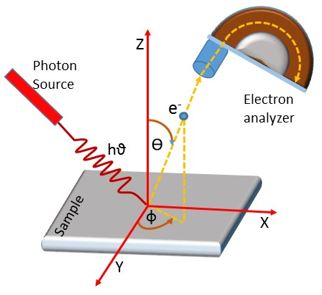
\includegraphics[width=0.5\textwidth]{ARPES}
                \caption{Versuchsanordnung zur Messung winkelaufgelöster Photoemissionsspektren. Aus~\cite{ARPES}.}
                \label{fig:ARPES}
            \end{figure}

            Die genaue Winkelverteilung der Elektronen wird bei der winkelaufgelösten Photoelektronenspektroskopie genauer untersucht.
            Hierzu wird vom Analysator nur ein kleiner Winkelbreich akzeptiert und der Winkel zwischen Probe und Analysator stets varriert.
            Schematisch ist dies auch in \autoref{fig:ARPES} dargestellt.
            Für jede Winkelkombination aus polarem $\theta$ und azimunthalen $\phi$ Winkel wird ein UPS Spektrum aufgezeichnet.
            Die entsprechenden Impulsvektoren lassen sich aus den Winkeln und der kinetischen Energie nach
            \begin{gather}
                k_\text{x} = \sqrt{\frac{2 \text{m}_\text{e} E_\text{Kin}}{\hbar^2}} \sin\theta \cos\phi \\
                k_\text{y} = \sqrt{\frac{2 \text{m}_\text{e} E_\text{Kin}}{\hbar^2}} \sin\theta \sin\phi
            \end{gather}
            berechnen~\cite{MM_4}.
            Wird für eine feste Energie über alle Winkel integriert und dies für jede gemessene Energie aufgetragen ergibt sich eine integriertes Spektrum.
            Dies hat die Bezeichnung \textit{electron density curve} (EDC), da sie die Zustandsdichte des Valenzbandes wiederspiegelt.

            Von der Seite der Theorie wird das ein Stufen Model der Photonelektronenemission verwendet, welches den Prozess der Photoemission besser beschreibt, aber nicht so anschaulich wie das drei Stufen Model ist.
            Es berücksichtigt unter Anderem, den Austrittswinkel der Elektronen (polar $\theta$ und azimuthal $\phi$) sowie den finale Zustand $\Psi_\text{f}$ mit einer Energie $E_\text{Kin}$.
            So ergibt sich die Photoelektronenintensität in entsprechende Richtung 
            \begin{equation}
                I(\theta, \phi, E_\text{Kin}) \propto \sum_i \abs*{\bigl<\Psi_\text{f}(\theta, \phi, E_\text{Kin})|\vec{A}\cdot\vec{p}|\Psi_\text{i}\bigr>}^2 \times \delta\left(E_\text{i}+E_\text{Kin}+\Phi-h\nu\right))
            \end{equation}
            vom Anfangszustand $\Psi_\text{i}$ in der Dipolapproximation~\cite{MM_2}.
            Durch die ebene Wellen Approximation des Endzustands ist der Photoelektronenstrom proportinal zur Fouriertransformation des Anfangszustandes.
            So ergibt sich unter Beachtung des Polarisationsfaktors $\abs*{\tilde{\Psi}_\text{i}(\vec{k})} \propto \frac{\sqrt{I_\text{i}(\theta, \phi)}}{\abs*{\vec{A}\cdot\vec{k}}}$.

    \section{2D Photoelektronen Mikroskopie} \label{sec:2D-PES}
        Die 2D Photoelektronen Mikroskopie ist eine sehr viel versprechende Technik, die für immer mehr Aufsehen in den letzten Jahren gesorgt hat.
        Der größte Vorteil liegt wohl in der Kombination von spektroskopischen Methoden und mikroskopischen Methoden.
        Zuerst wurde dies 1933 durch E. Brüche entdeckt, der eine Zinkplatte mit Hilfe von Photoelektronen und einer magnetischen Linse auf einem Leuchtschirm abbildete~\cite{bruche_elektronenmikroskopische_1933}.
        Sie nutzt die Prinzipien der Energie- und Impulserhaltung um Bilder der Proben im Realraum oder Impulsraum aufzulösen.

        \begin{figure}
            \centering
            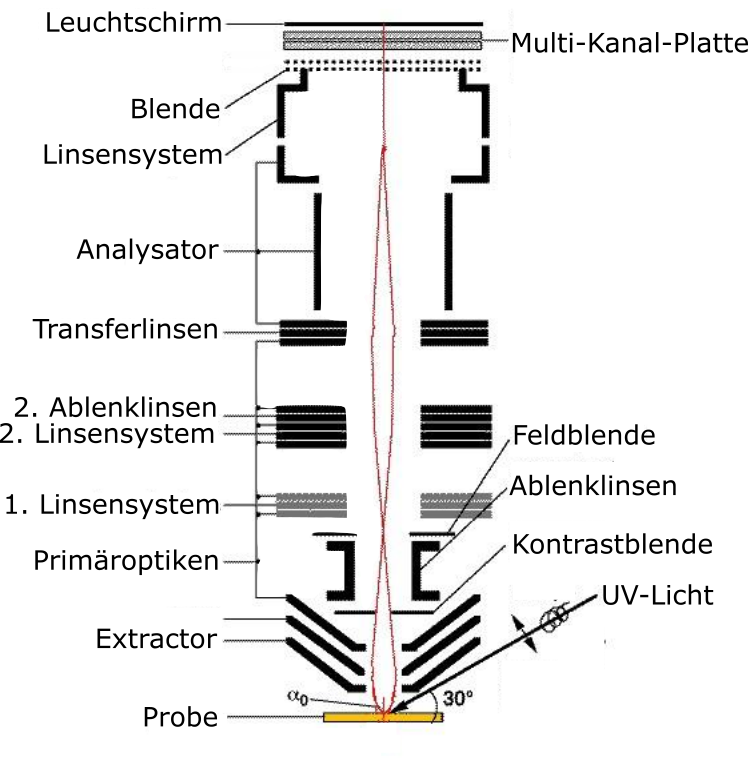
\includegraphics[width=0.6\textwidth]{PEEM_schemaneu.png}
            \caption{Vereinfachter Aufbau eines 2D Photoelektronen Mikroskopes. Vorlage aus~\cite{KUCH}, modifiziert.}
            \label{fig:MM}
        \end{figure}
        Ein exemplarischer Aufbau ist in \autoref{fig:MM} zu sehen.
        Die durch die Photonen angeregten Elektronen werden durch ein starkes elektrisches Feld von einigen \si{\kilo\volt} von der Probe zum Analysator hin beschleunigt.
        Das Extraktorfeld kann bis auf \SI{29}{\kilo\volt} erhöht werden.
        Durch diese große Spannung zwischen Probe und Extraktor ist es möglich einen großen Sichtbereich im Impulsraum abzudecken.
        Dies ist nötig, da durch den streifenden Einfall der Photonen und der Abberation der elektrostatischen Linsen nur einen kleinen Akzeptanzwinkel zur Verfügung stehen würde.
        Wichtig bei der Kathodenlinse ist, dass das Feld zwischen Probe und Linse sehr homogen ist, damit der Austrittswinkel erhalten bleibt, dies hat zur Folge, dass die Probe auch eine möglichst ebene Oberfläche aufweisen muss.
        Anschließend werden die Elektronen durch elektrostatische Linsen fokussiert und durch einzelne optische Elemente geleitet.
        Zusätzlich gibt es im Linsensystem noch elektrostatische Verschiebungslinsen, welche den Strahl ablenken und zentrieren.
        Die ersten Linsen sind so konzipiert, dass die Bildebene und die hintere Brennebene immer an der selben Position auftreten.
        An diesen beiden Stellen kann eine Blende eingestzt werden, die entscheidet ob sich ein Bild im Realraum oder im Impulsraum auf den Detektor abbildet.

        Im Anschluss an das erste Linsensystem folgt ein weiters Linsensystem aus elektrostatischen Linsen, welche das Bild auf den Ausgang des Linsensystems fokussieren.
        Hier befinden sich zwei magnetische Verschiebungslinsen um Drift zu korrigieren.
        Im Anschluss gehen die Elektronen in ein Transferlinsensystem über, welches dafür sorgt, dass ein einszueins Abbild auf die Eingangsblende des Analysators trifft.
        Die Eingangsblende kann in ihrer Größe varriert werden, sodass nur ein Teil der Elektronen in den Analysator eintritt.
        Je kleiner die Blende gewählt wird, desto besser ist die Energieauflösung aber so kleiner die Gesamtintensität.
        Als Energieanalysator kommt ein hemisphärischer Analysator zum Einsatz.
        Bei dem hemisphärischer Analysator werden die Elektronen zwischen zwei Halbkugeln durch ein statisches elektrisch Feld auf eine Kreisbahn gezwungen.
        Dabei ist das Feld so gewählt, dass nur die mit der richtigen kinetischen Energie eintretenden Elektronen auf die Austrittsblende abgebildet werden.
        % Ferner wird der Analysators so eingestellt, dass Elektronen mit einer Energie von \SI{50}{\milli\electronvolt} um die eingestellte Energie den Analysator passieren können, dies ist die Pass-Energie.
        
        Nach dem Detektor gibt es eine weiter Linseneinheit, welche zusammen mit einer Blende das gewünschte energieaufgelöst Bild auswählt und es auf die Detektorgröße aufweitet.
        Anschließend durchlaufen die Elektronen eine Mikrokanalplatte (eine Art Elektronenvervielfacher) und prallen auf den Phosphorschirm, der an den entsprechenden Stellen aufleuchtet.
        Durch die Kamera wird dieses Leuchten regestriert und das räumliche oder rekrusive Bild kann rekostruiert werden~\cite{SPECS-MM}.
        % Bei dem Detektor handelt es sich um eine CMOS Kamera die das Bild der auf den Leuchtschirm auftreffenden Elektronen aufnimmt.
        CCD (\textit{Charge Coupled Device}) Detektoren sind ein Standard bei ARPES Messungen, sie integrieren die analoge Photonenintensitäten oder einzelne Lichtblitze werden aufgezeichnet.
        Einer der Nachteile ist die geringe Abtastrate auf Grund der hohen Erholungszeit.
        Hier wird allerdings eine CMOS (\textit{Complemantary metal-oxid-semiconductor}) Kamera verwendet.
        % Dabei wird ein einzelnes Bild in nur wenigen Millisekunden erfasst, dies ist durch die Kombination von Kamera und Grafigprozessor möglich.
        Der Vorteil der CMOS Kamera Technik gegenüber der klassischen CCD  Kamera Technik ist, die Erfassung der wahren Pulszählraten~\cite{CMOS}.
        
        Es gibt zwei verschiedene Betribsmodi welche ferner erläutert werden.
        \begin{figure}
            \centering
            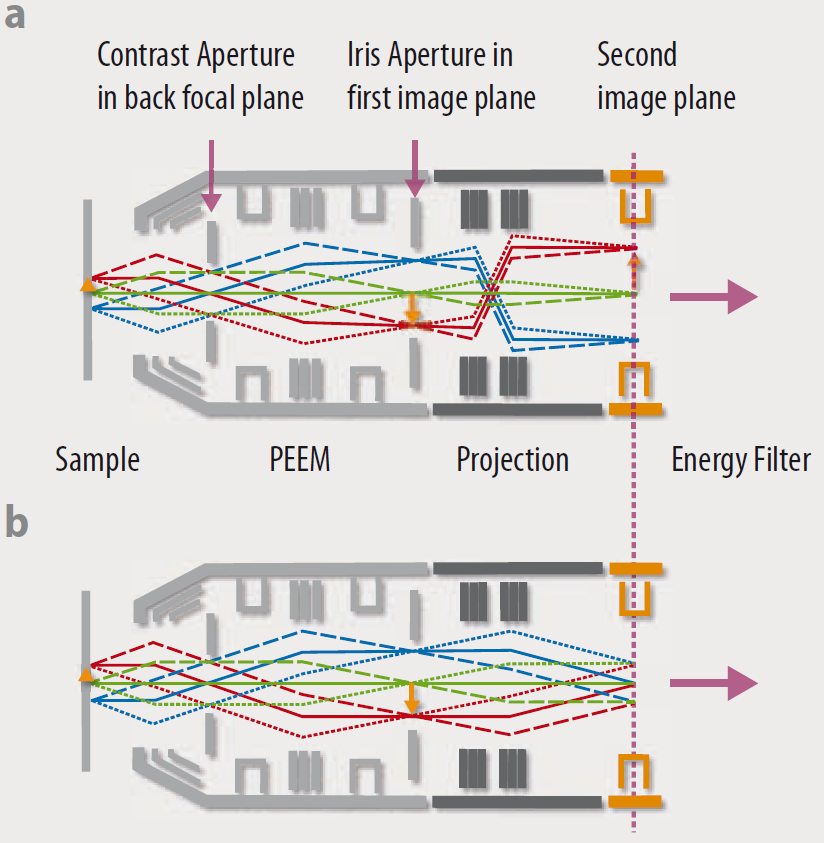
\includegraphics[width=0.5\textwidth]{Real_k.PNG}
            \caption{Die verschiedenen Konfiguration der Blenden um zwischen Realraum und Impulsraum Bild umzuschalten. Aus~\cite{Focus}.}
            \label{fig:real_k}
        \end{figure}
        Für den Impulsraum ist dies in \autoref{fig:real_k}\,a und für den Realraum in \autoref{fig:real_k}\,b dargestellt.
        Vorteil der Umschaltung zwischen den Modis ist, dass auf sehr kleinen Bereichen die im Realraum bestimmt wurden dann auch Messungen im reziproken Raum durchgeführt werden können.


        \subsection{Impulsraum Aufnahmen}
            Um ein Bild im Impulsraum aufzunehmen wird die Blende in der Bildebene eingefahren, die so genannte Feldblende (\textit{field aperture}).
            Durch die Blende wird ein Ausschnitt auf der Probe ausgwählt, von der die emittierten Elektronen erfasst werden.
            Bei einem Blendendurchmesser von \SI{20}{\micro\meter} und der Vergrößerung (\textit{magnification}) von~\num{5} ist der ausgewählt Bereich etwa \SI{4}{\micro\meter} groß.
            Bei der Aufnahme im Impulsraum wird bei der gesamten Abbildungsoptik der Austrittswinkel erhalten.
            So wird auf die Eintrittsblende des Analysators das Beugungsbild abgebildet.
            Das verwendete Mikroskop kann einen Austrittswinkel von biszu $\pm\SI{90}{\degree}$ erfassen für eine Energie kleiner als \SI{50}{\electronvolt}~\cite{SPECS-MM}.
            Für größere kinetische Energien wird das Sichtfeld auf $\pm\SI[per-mode=reciprocal]{3.6}{\per\angstrom}$ beschränkt.
            Dabei spielt es keine Rolle wo auf der Probe die Elektronen emittiert werden.

            Dies wird auch Impuls Mikroskopie (\textit{Momentum Microscopy}) bezeichnet.
            Bei der Impuls Mikroskopie ist die zeitgleich Erfassung des polaren und azimuntalen Austrittswinkel von großer Bedeutung. 
            So entsteht durch die zusätzlich Sortierung der Elektronen nach ihrer kinetischen Energie ein dreidimensionaler Datensatz.
            Wird über das gesamte Bild also alle Winkel integriert so ergibt sich die Kurve der Elektronendichte.

        \subsection{Realraum Aufnahmen}
            Es ist ferner möglich Bilder im Realraum aufzunehmen.
            Dies geschieht durch Einsetzen einer Blende in dem hinteren Brennpunkt, die Kontrastblende (\textit{contrast aperture}).
            Dabei können sehr kleine Spots von \SIrange{50}{200}{\micro\meter} ausgewählt werden.
            Um den Kontrast im Bild zu erhöhen werden nur Elektronen mit einem bestimmten Austrittswinkel für die Erstellung des Bildes erfasst.
            Mit Hilfe der Kontrastblenden kann eine Auflößung von einigen \si{\nano\meter} erreicht werden. 
            Auf dem Eintrittsspalt des Energieanalysators wird das Bild der Oberfläche projeziert.
            Das Bild wird bei festen Energiefilter-Einstellungen aufgenommen.
            Der Modi wird auch als PEEM (\textit{Photon emitted electron microscopy}) bezeichnet.

        \subsection{Erweiterungen}
            Als Erweiterung der 2D Photoelektronen Mikroskopie sind auch zeitaufeglöste Messungen möglich.
            Hierbei erfolgt die Anregung mit zwei zeitlich versetzten Pulsen. 
            Dabei regt der erste Puls die Elektronen in einen höheren Zustand an und der zweite Puls löst diese dann aus.
            So ist es auch möglich zuvor unbesetzte Zustände (zwei Photonenemission) zu untersuchen.
            Wird der zeitliche Versatz zwischen den beiden Pulsen varriert so ist auch die Lebensdauer der Zustände abschätzbar.
            Für die gepulste Photonenquellen würde sich ein Flugzeit (TOF, \textit{Time of flight}) Analysator besser eignen.
            In einem TOF Analysators wird die kinetische Energie aus der Flugzeit der Elektronen bestimmt, weswegen es nur für gepulste Photonenquellen möglich ist.
            Der Vorteil liegt darin, dass direkt ein ganzer Datensatz für alle Impuls- und Energiewerte erfasst werden kann.

            Mögliche Erweiterung wäre auch die Elektronen nach der Energieselektion auch noch nach ihrem Spin zu sortieren.
            So lassen sich die magnetischen Eigenschaften genauer veranschaulichen.
        
    \section{Molekül Orbital Tomographie} \label{sec:MOT}
        Die Molekül Orbital Tomographie vereinigt die Vorteile der Impulsmikroskopie mit der Dichtefunktionaltheorie (DFT) um Molekülorbitale zu identifizieren.
        Aus der Theorie können die Orbitale der Moleküle in der Gasphase im Realraum berechnet werden~\cite{database}.
        Werden diese dann Fourier transformiert, so ergibt sich die Aufenthaltswahrscheinlichkeiten der Elektronen abhängig von ihrem Impuls.
        Nun können die Moleküle bei einer bestimmten kinetischen Energie geschnitten werden und es ergibt sich ein zweidimensionales Bild~\cite{brandstetter_kmappy_2021}.
        Ferner kann auch die Wechselwirkungswahrscheinlichtkeit mit der verwendeten Photonenenergie berücksichtigt werden.
        Aus Messungen im Impulsraum können dann durch einen Vergleich die Molekülorbitale zugeordnet werden.
        Dies ist nur möglich, wenn sich die Moleküle ordnen wie z.B. auf einigen metallischen Oberflächen.

        Wie bereits in \autoref{sec:ARPES} erwähnt ist der Photoelektronenstrom in der Approximation einer ebenen Welle des Endzustands durch die Fouriertransformation des Anfangszustands verknüpft.
        So kann also durch erneute Fouriertransformation aus dem Impulsraum zurück in den Realraum auf die Molekülorbitale geschlossen werden~\cite{MM_2}.

        Unter der Beachtung von: (i)~der Emission von $\pi$-Orbitalen großer Moleküle, (ii)~dass der Winkel zwischen Polarisationsvektor $\vec{A}$ und Richtung der austretenden Elektronen $\vec{k}$ klein ist und (iii)~die Moleküle aus leichten Atomen bestehen, ist es möglich mit der Annahme der ebenen Welle und DFT die Molekülstruktur im Realraum zu berchnen \cite{MM_2}.
        \begin{figure}
            \centering
            \begin{subfigure}{0.3\textwidth}
                \centering
                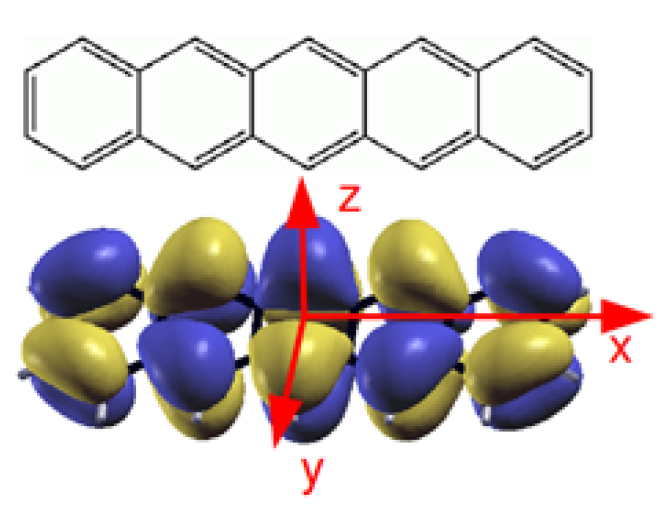
\includegraphics[width=0.9\textwidth]{DFT1.PNG}
                \caption{}
                \label{fig:DFT1}
            \end{subfigure}
            \begin{subfigure}{0.3\textwidth}
                \centering
                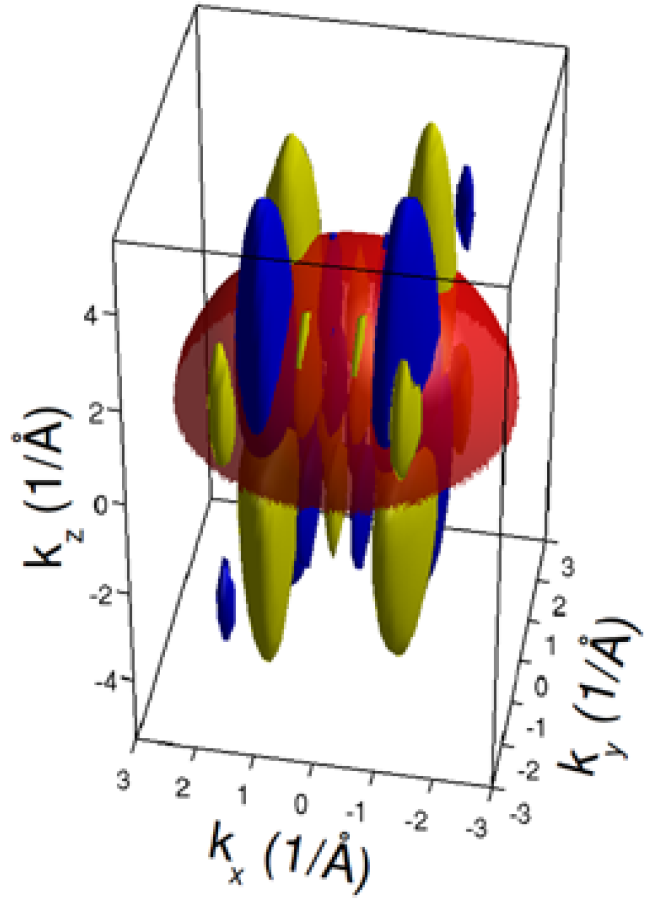
\includegraphics[width=0.9\textwidth]{DFT2.PNG}
                \caption{}
                \label{fig:DFT2}
            \end{subfigure}
            \begin{subfigure}{0.3\textwidth}
                \centering
                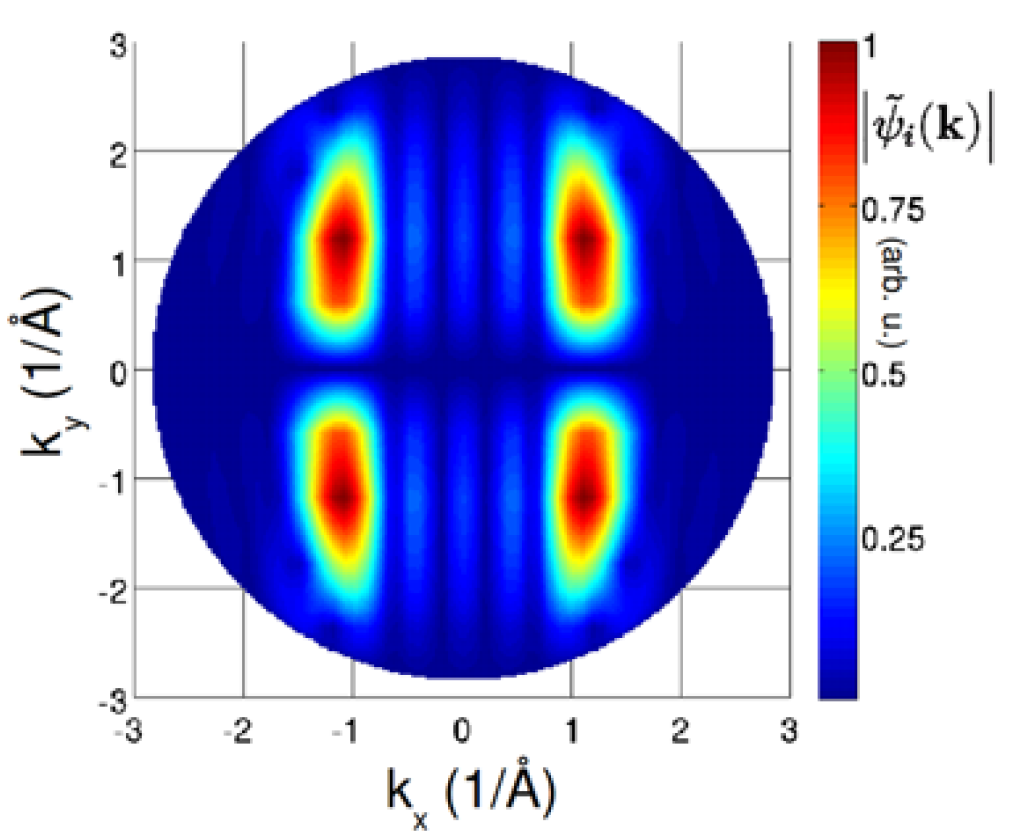
\includegraphics[width=0.9\textwidth]{DFT3.PNG}
                \caption{}
                \label{fig:DFT3}
            \end{subfigure}
            \caption{In \subref{fig:DFT1} ist die sich aus der Dichtefunktionaltheorie (DFT) ergebene Struktur von Pentacene gezeigt.
            Die durch Fouriertransformation gewonnen Orbitalstruktur im reziproken Raum \subref{fig:DFT2}.
            \subref{fig:DFT3} die Projektion der Fouriertransformation der Molekülorbitale für eine feste kinetische Energie.
            Aus~\cite{MM_2}}
            \label{fig:DFT}
        \end{figure}
        Dies ist beispielhaft in \autoref{fig:DFT1} für Pentacene geschehen.
        Wird nun eine Fouriertransformation durchgeführt ergibt sich das Bild \autoref{fig:DFT2}.
        Schließlich wird die Fouriertransformation entlang einer Ebene konstanter kinetischer Energie, was der roten Hemisphäre in \autoref{fig:DFT2} entspricht, geschnitten.
        Es ergibt sich die Projektion in \autoref{fig:DFT3}.
        Nun kann diese Projektion mit der gemessenen Photoelektronenintensitäten verglichen werden.

        Mit Hilfe der Molekülorbitaltomographie ist es nicht nur möglich Merkmale im Valenzband einzelnen Molekülorbitalen zuzuordnen, sondern auch ihre Ausrichtung auf dem Substraht zu bestimmen.
        So kann zum Beispiel die Neigung der Moleküle in eine Verschiebung der projezierten Molekülorbitalmerkmale in den Impulsbildern enden.
        Auch kann die Ausrichtung der Moleküle entlang der Symmetrien des Substrahtes bestimmt werden.

    \section{Versuchsaufbau}
    \label{sec:Versuchsaufbau}
        \begin{figure}
            \centering
            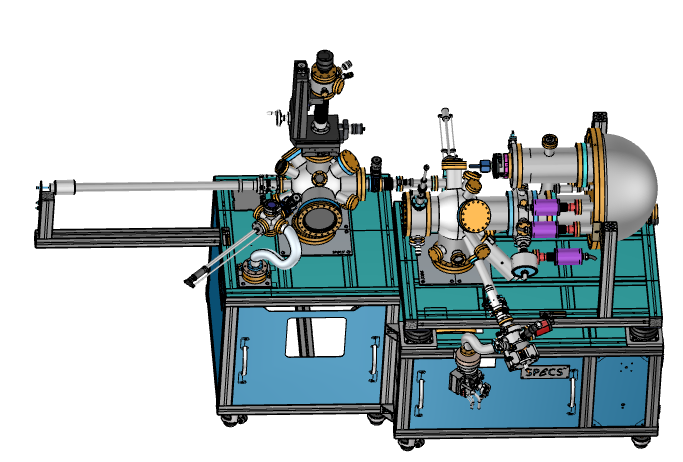
\includegraphics[width=0.7\textwidth]{MM.png}
            \caption{Der für die durchgeführten Experimente verwendete Aufbau.}
            \label{fig:aufbau}
        \end{figure}
        Um die in dieser Arbeit untersuchten Proben zu präperieren und zu untersuchen wird der Versuchsaufbau in \autoref{fig:aufbau} verwendet.
        Dieser besteht aus einer Präperationskammer (links im Bild) und dem 2D Photoelektronen Mikroskop KREIOS 150MM von SPECS (rechts im Bild).

        Für die Reinigung der Probe steht eine Ionenquelle zur Verfügung, um die Probe mittels ioneninduzierter Zerstäubung zu reinigen.
        Auf dem Manipulator, mit dem die Probe im Ultrahochvakuum verfahren werden kann, ist eine Elektronenstoßheizung montiert, um die Probe aufzuheizen.
        Die Präperationskammer ist mit einer LEED-Optik ausgestattet um die Oberflächenbeschaffenheit zu kontrollieren.
        Ferner befindet sich noch ein Leckventil für Sauerstoff, sowie Molekül- und Metallaufdampfer an der Kammer.
        
        Vor der Extraktorlinse des 2D Photoelektronen Mikroskopes befindet sich eine 6-Achsen-Piezostage (Hexapod) mit der die Probe in Position gebracht und ausgerichtet werden kann.
        Messungen erfordern eine exakte Ausrichtung der Oberflächennormalen parallel zur Linsenachse und ferner einen Abstand von \SI{4}{\milli\meter} zum Extraktor.
        Mit dieser Positioniereinheit kann die Probe auch auf unter \SI{10}{\kelvin} abgekühlt werden.
        Als Photonenquelle steht eine Helium-Gasentladungslampe bereit, welche größtenteils Photonen der He-I-Linie (\SI{21.22}{\electronvolt}) emittiert~\cite{UVS}.
\chapter{Ergebnisse}
    Innerhalb diese Kapitels geht es zunächst um die Vorbereitung der Proben.
    Weiter geht es es um den Umgang mit dem dreidimensionalen Datensatz sowie dessen Bearbeitung.
    Die verschiedenen extrahierten Darstellungen werden dann aufgenommen und analysiert.
    In dieser Arbeit untersuchten Gold und Nickeloxid Proben wurden alle in dem Versuchsaufbau aus \autoref{sec:Versuchsaufbau} vorbereitet und vermessen.
    Die Eisenoxid Proben wurden an der NanoESCA Beamline am Synchrotron Elettra in Triest präperiert und charakterisiert \footnote{Näheres zu diesem Versuchsaufbau und der Behandlung der Daten kann in \cite{ma-DJ} gefunden werden.}.

    \section{Gold}
        \begin{figure}
            \centering
            \begin{subfigure}{0.48\textwidth}
                \centering
                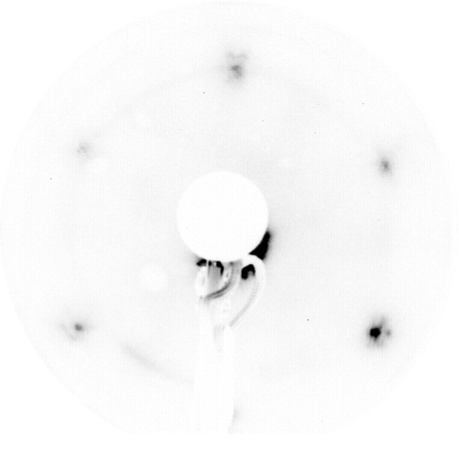
\includegraphics[height=5cm]{./content/pictures/Au/2021_06_08_002_Au(111)_75eV}
                \subcaption{Gold (111) bei einer Elektronenenergie von \SI{75}{\electronvolt}.}
                \label{fig:LEED_Au}
            \end{subfigure}
            \begin{subfigure}{0.48\textwidth}
                \centering
                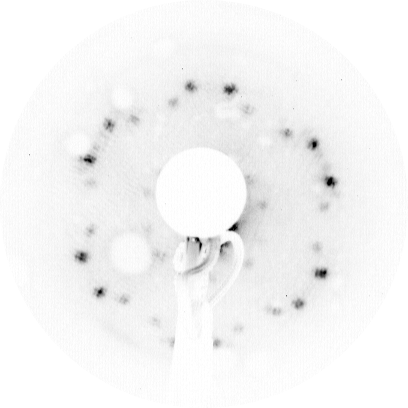
\includegraphics[height=5cm]{./content/pictures/Au+5A/021_Au(111)+5A(40)_16eV.png}
                \subcaption{Eine Monolage Pentacene auf dem sauberen Gold bei einer Energie von \SI{16}{\electronvolt}.}
                \label{fig:LEED_Au+5A}
            \end{subfigure}
            \caption{Die LEED-Bilder für die Kalibrierung des Pentacene.}
        \label{fig:Substrate}
        \end{figure}
        Zunächst geht es hier um das Substrat auf dem später der antiferromagnetische Nickeloxidfilm gewachsen wird.
        Das Substrat wurde zunächste mehrer Male durch ioneninduziertes Zerstäuben und anschließendes Aufheizen auf \SI{500}{\celsius} gereinigt.
        Es ergibt sich eine wohldefinierte Struktur der Oberfläche, was sich ebenfalls in dem Beugungsbild der niederenergetischen Elektronen in \autoref{fig:LEED_Au} erkennen lässt.
        Ferner sind scharfe Spots zu erkennen, ebenso wie die charakteristische kleineren Spots um die Hauptspots, die von der Fischgräten-Rekonstruktion herrühren.
        Die unterschiedlichen Intensität der einzelnen Reflexe rühr ebenfalls von der Rekonstruktion her.

        \begin{figure}
            \centering
            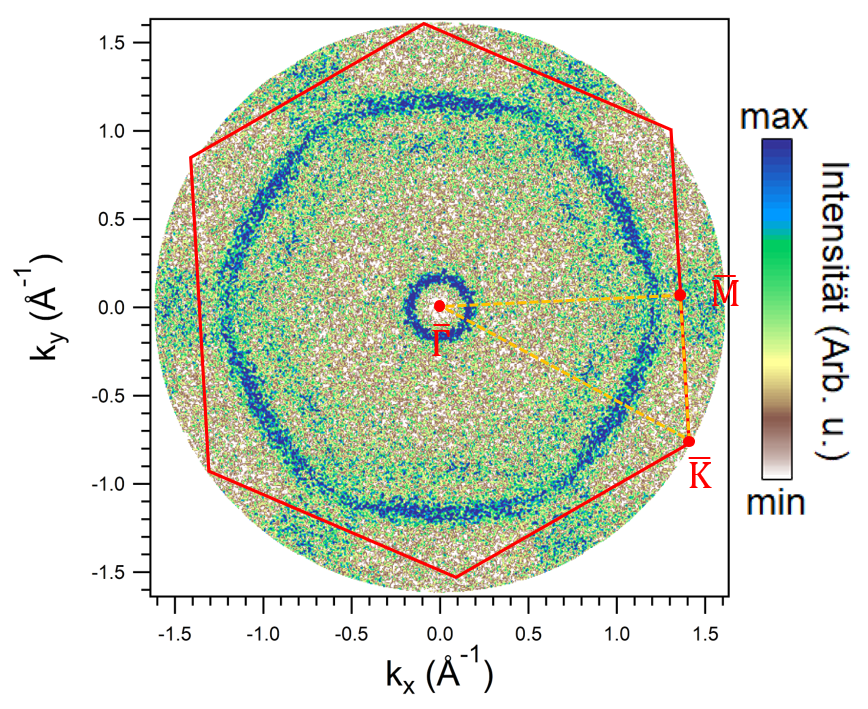
\includegraphics[width=0.5\textwidth]{./content/pictures/Au/BZ_Au.png}
            \caption{Die gemessene Winkelverteilung von Gold (111) an der Fermifläche.
            Eingezeichnet in rot ist die erste Brillouinzone und drei Hochsymmetriepunkte, entlang deren Richtung der Stack für die Bandstruktur geschnitten wird.}
            \label{fig:BZ_Au}
        \end{figure}
        \begin{figure}
            \centering
            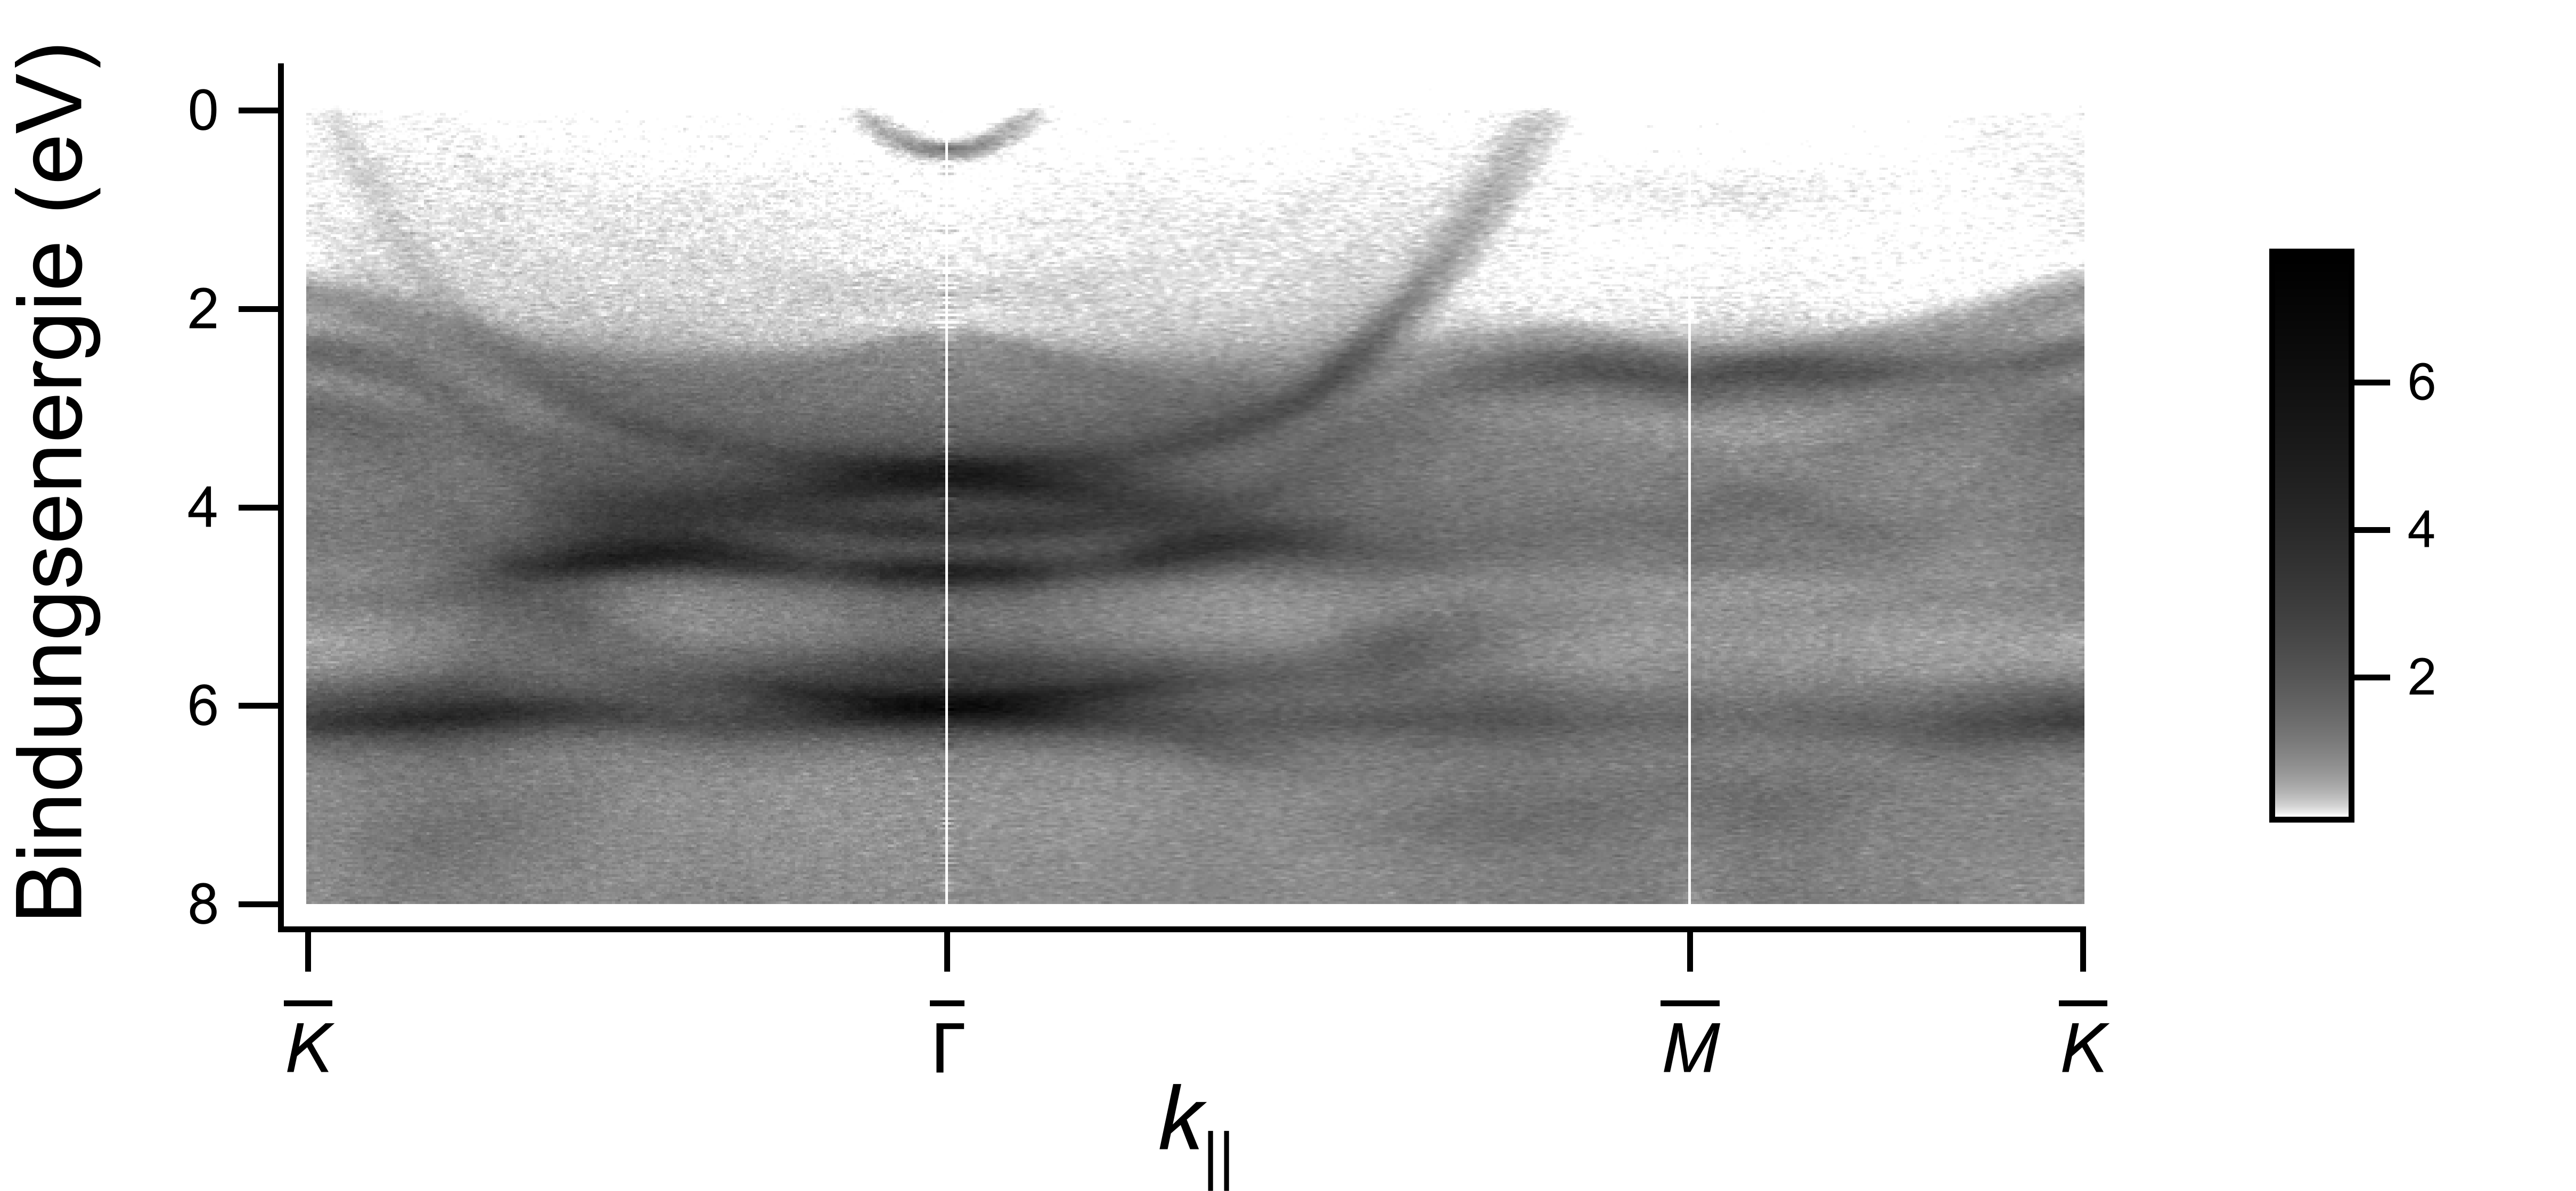
\includegraphics[width=0.8\textwidth]{./content/pictures/Au/Band_Au111.png}
            \caption{Die gemessene Bandstruktur von Gold (111).}
            \label{fig:Band_Au}
        \end{figure}
        Die Eigenschaft, dass Gold einen Oberflächenzustand besitzt ist nützlich um festzustellen ob es sich um eine gut präperierte Oberfläche handelt.
        Der Oberflächenzustand lässt sich in \autoref{fig:BZ_Au} klar erkennen.
        Zusätzlich ist die erste Brillouinzone eingetragen sowie einige Hochsymmetriepunkte.
        Durch Schneiden entlang der Linien zwischen den Hochsymmetriepunkten ergibt sich die Bandstruktur, welche in \autoref{fig:Band_Au} dargestellt ist.
        Die Bindungsenergie wurde ermittelt in dem die Photonenenergie von \SI{21.22}{\electronvolt} angenommen wurde und die Fermikante des Goldes bei \SI{16.55}{\electronvolt} in einem winkelintegrierten Spektrum gefittet wurde.
        Damit wird die Austrittsarbeit des Analysators zu \SI{4.72}{electronvolt} bestimmt, nur dies fließt dann noch in die Gleichung \ref{eqn:Photoeffekt} ein.
        Dies ist vorallem für spätere messungen des Nickeloxidfilms wichtig, da es sich hierbei um einen Isolator handelt und somit die Fermienergie in den Bandlücke liegt.
        Wird die gesamte Länge des Spektrums betrachtet, also der Energieunterschied zwischen Fermikante und Ende des Sekundärelektronen, so lässt sich die Austrittsarbeit der Probe bestimmen.
        Für Gold lässt sich die Austrittsarbeit auf \SI{5.46}{\electronvolt} ermitteln, was in der selben Ornung wie Literaturwerte liegt~\cite{Hüfner}.

        \begin{figure}
            \centering
            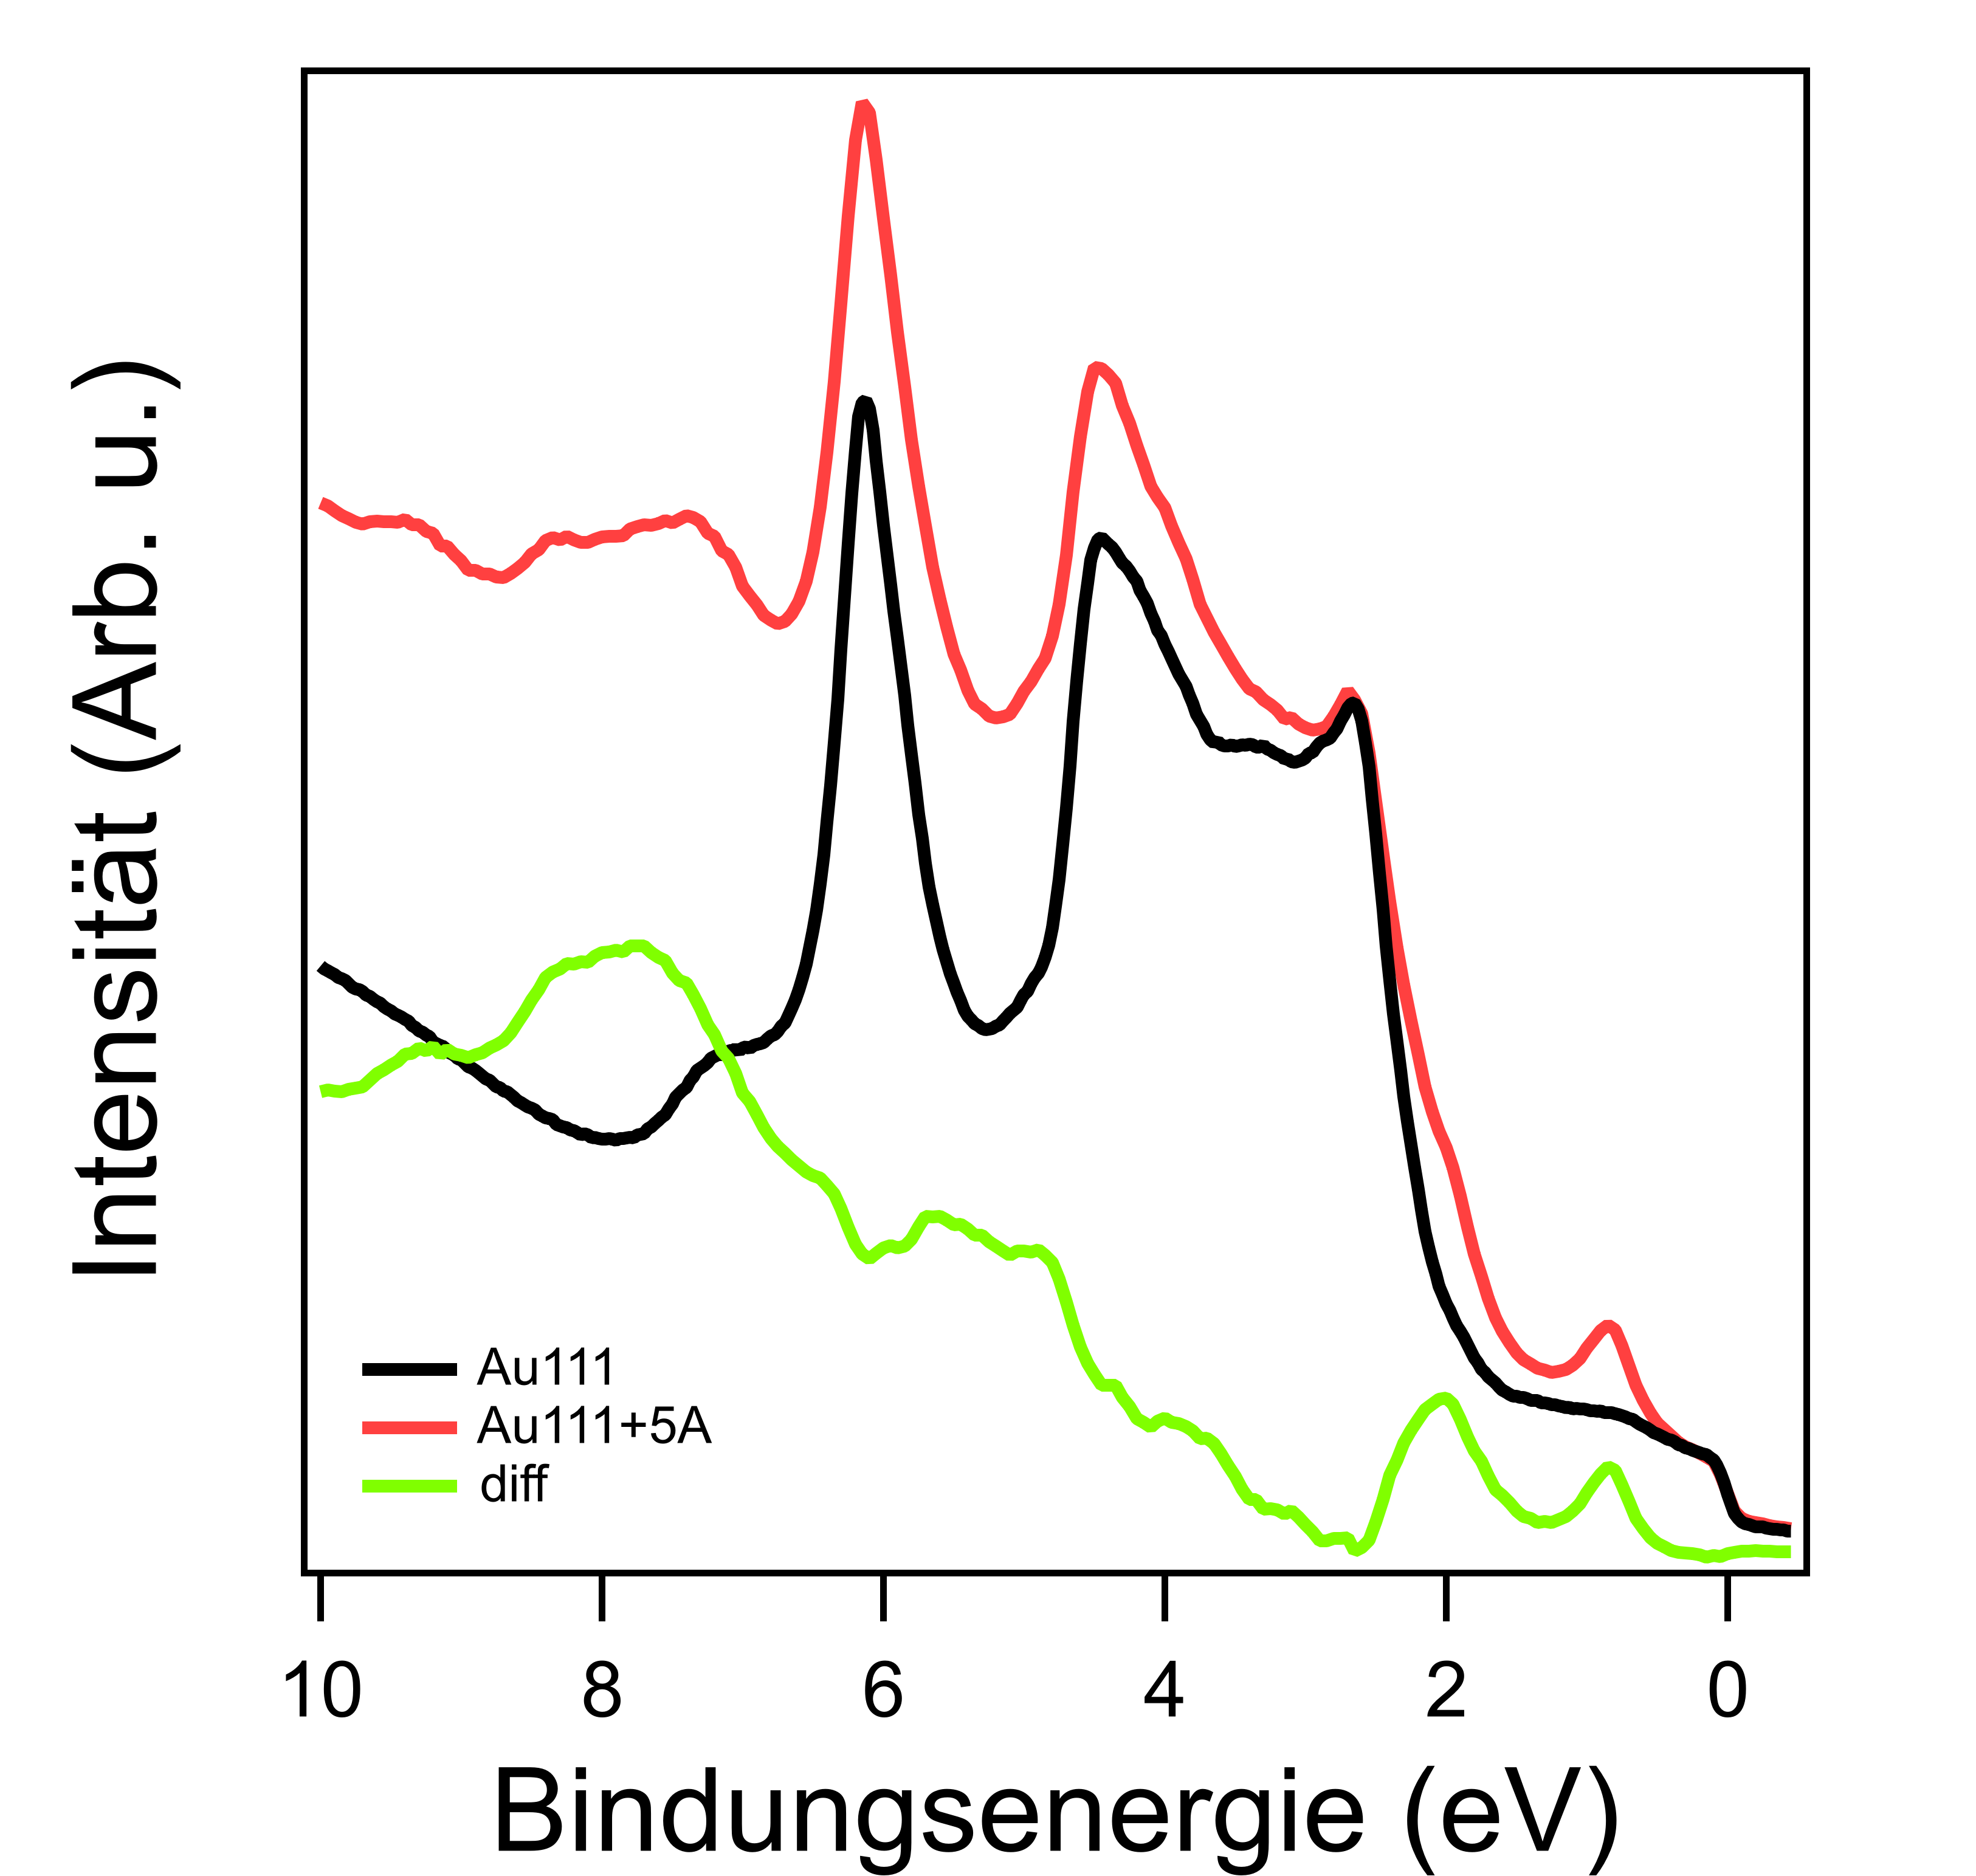
\includegraphics[width=0.5\textwidth]{./content/pictures/Au+5A/EDC_Au_5A.png}
            \caption{Die integrierten Spektren für reines Gold, Gold mit einer Monolage Pentacene und deren Differenz.}
            \label{fig:EDC_Au+5A}
        \end{figure}
        Das Goldsubstrat eignet sich ebenfalls zur Kalibrierung der Monolage von Pentacene, da bereits bekannt ist, dass sich diese flach auf der Oberfläche ordnet \cite{5A_1}.
        Bei der Wechselwirkung mit dem Substrat handelt es sich um die Physisorption durch einen Substrat-Molekülabstand von \SI{3.28}{\angstrom} \cite{5A_1}.
        % Es ergibt sich so das LEED-Bild in \autoref{fig:LEED_Au+5A}, was auch die bekannte \textbf{Überstruktur} (5A_1, 5A_5) aufweist.
        Schaut man sich das winkelintegrierte Spektrum im Bereich der Valenzzustände in \autoref{fig:EDC_Au+5A} an, so sind auch deutlich Elemente zu erkennen, die durch die Molekühle hervorgerufen werden.

        \begin{figure}
            \centering
            \begin{subfigure}[t]{0.48\textwidth}
                \centering
                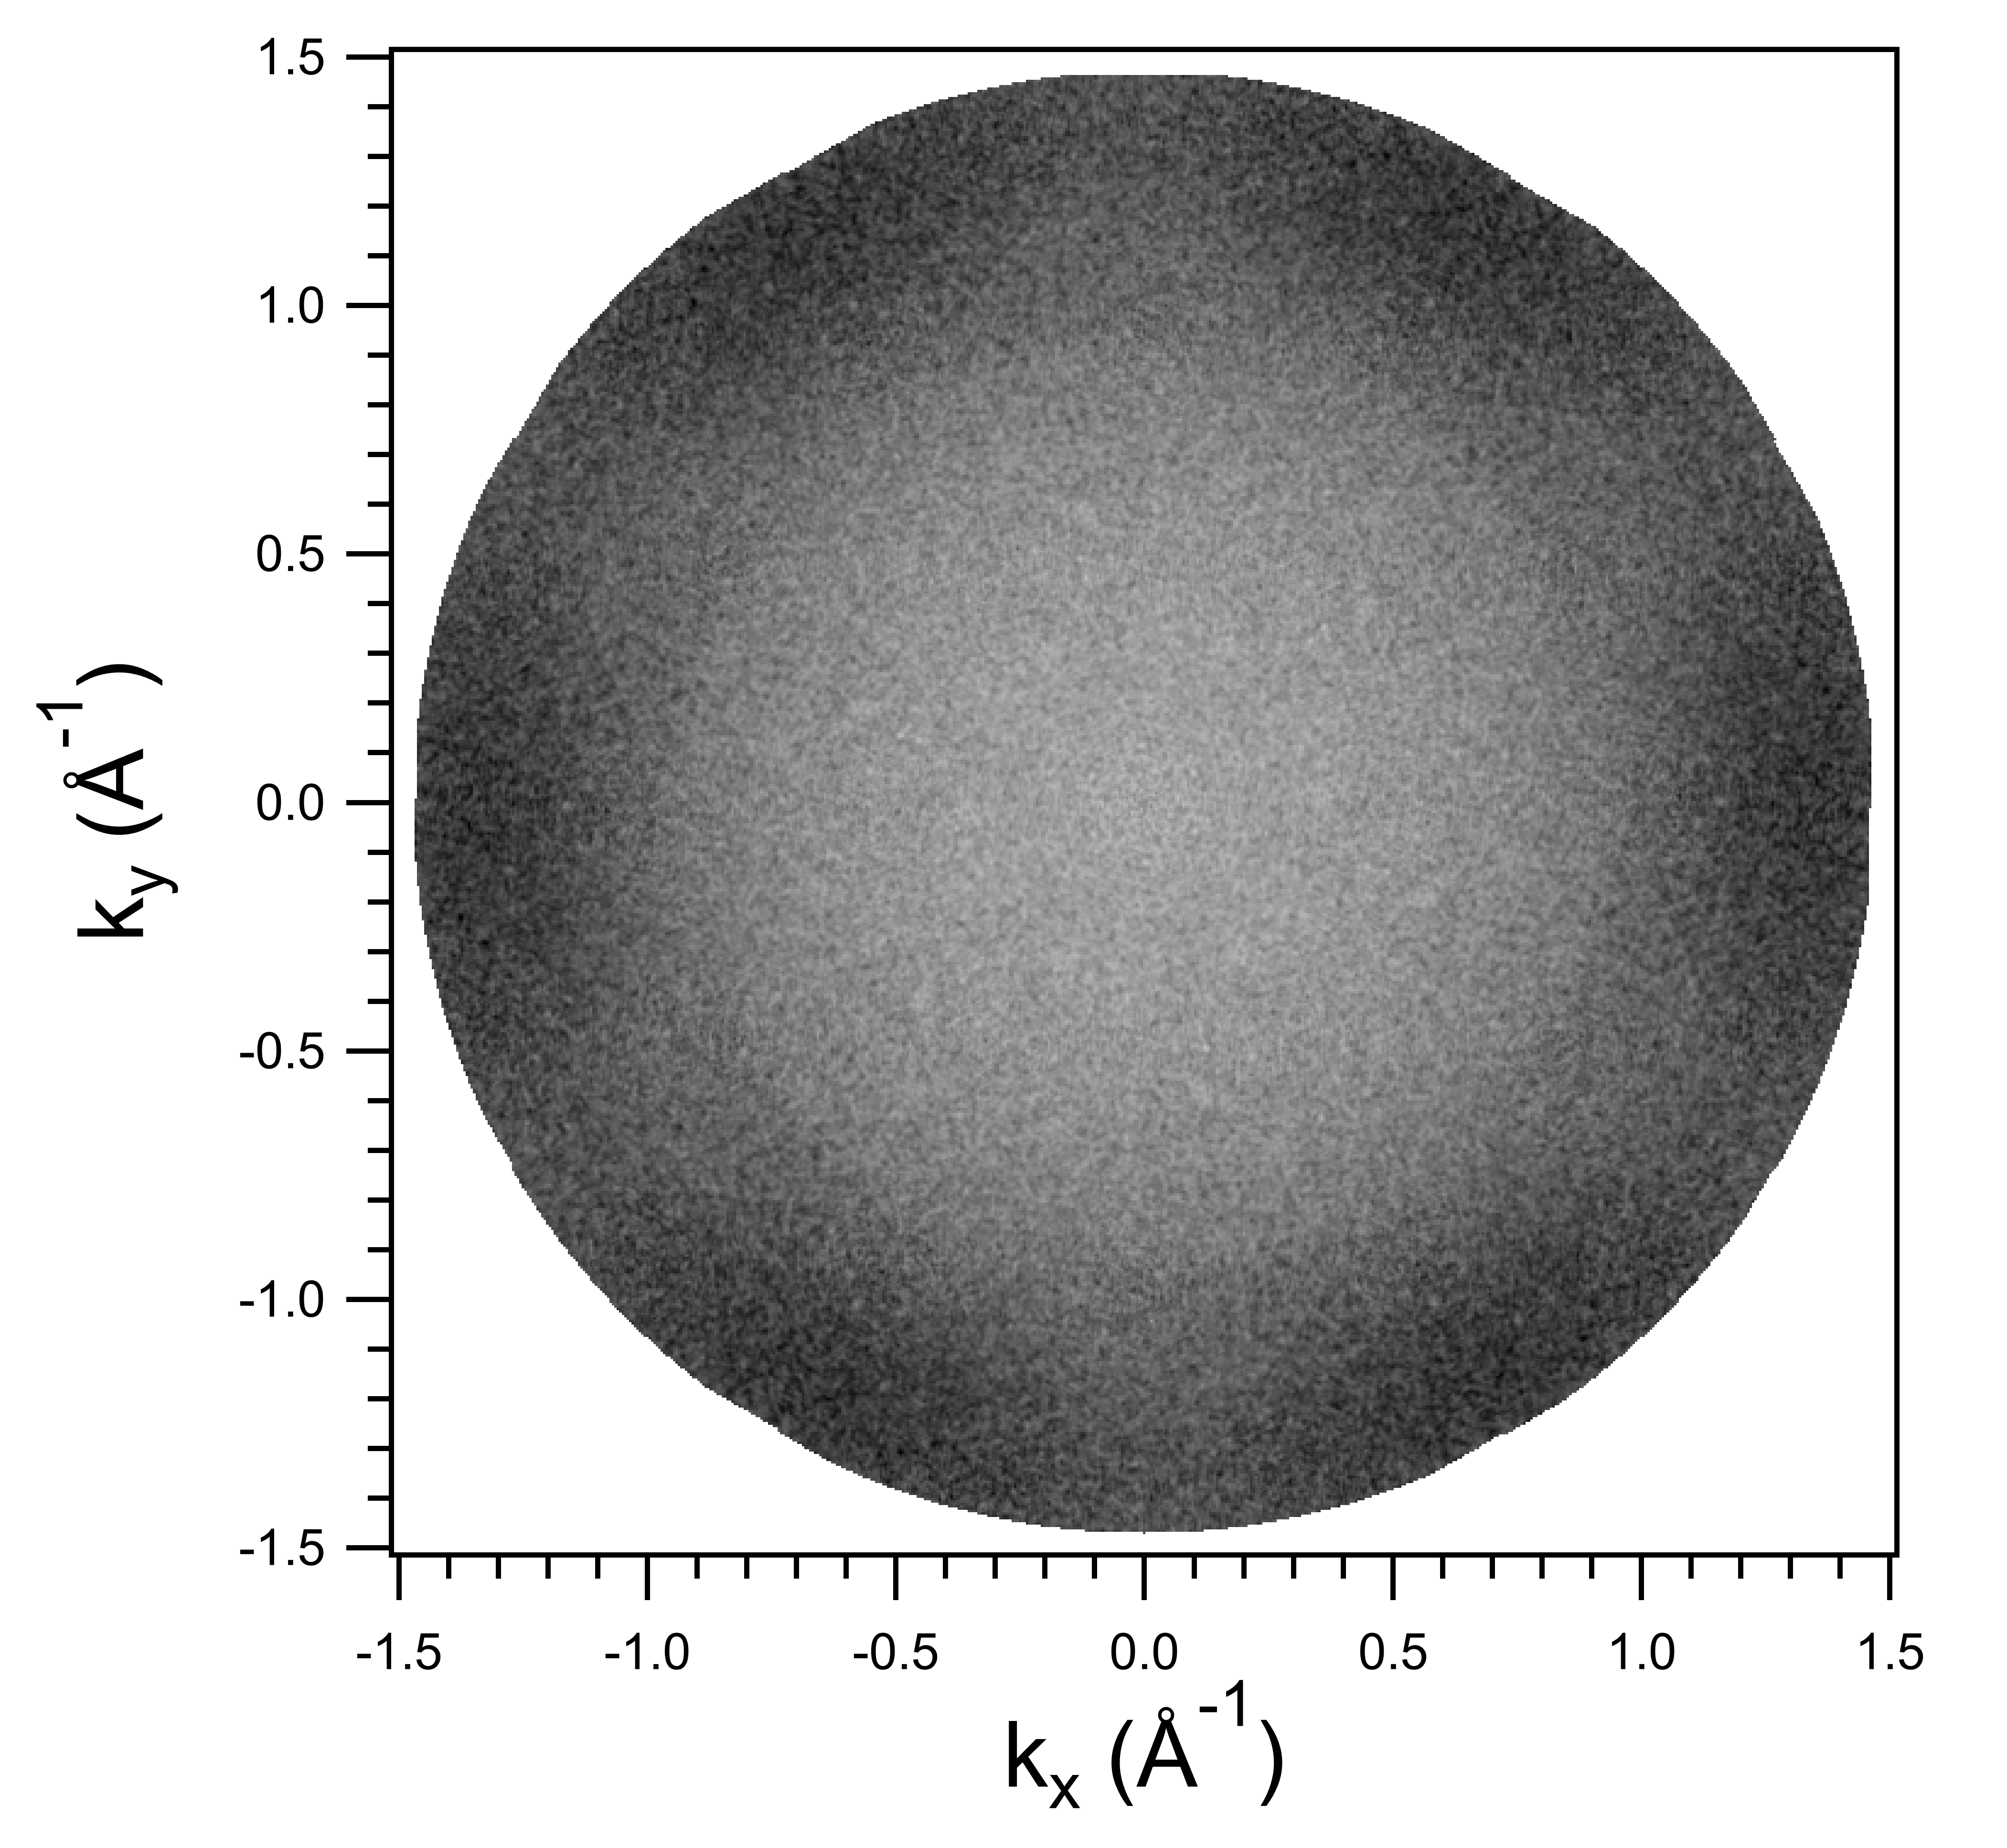
\includegraphics[height=5cm]{./content/pictures/Au+5A/IMAGE_2021_06_17_005_BE0_8}
                \subcaption{Gemmesen, symmetrisiertes Bild bei einer Bindungsenergie von \SI{0.8}{\electronvolt}.}
                \label{fig:MOT_Au+5A_exp}
            \end{subfigure}
            \begin{subfigure}[t]{0.48\textwidth}
                \centering
                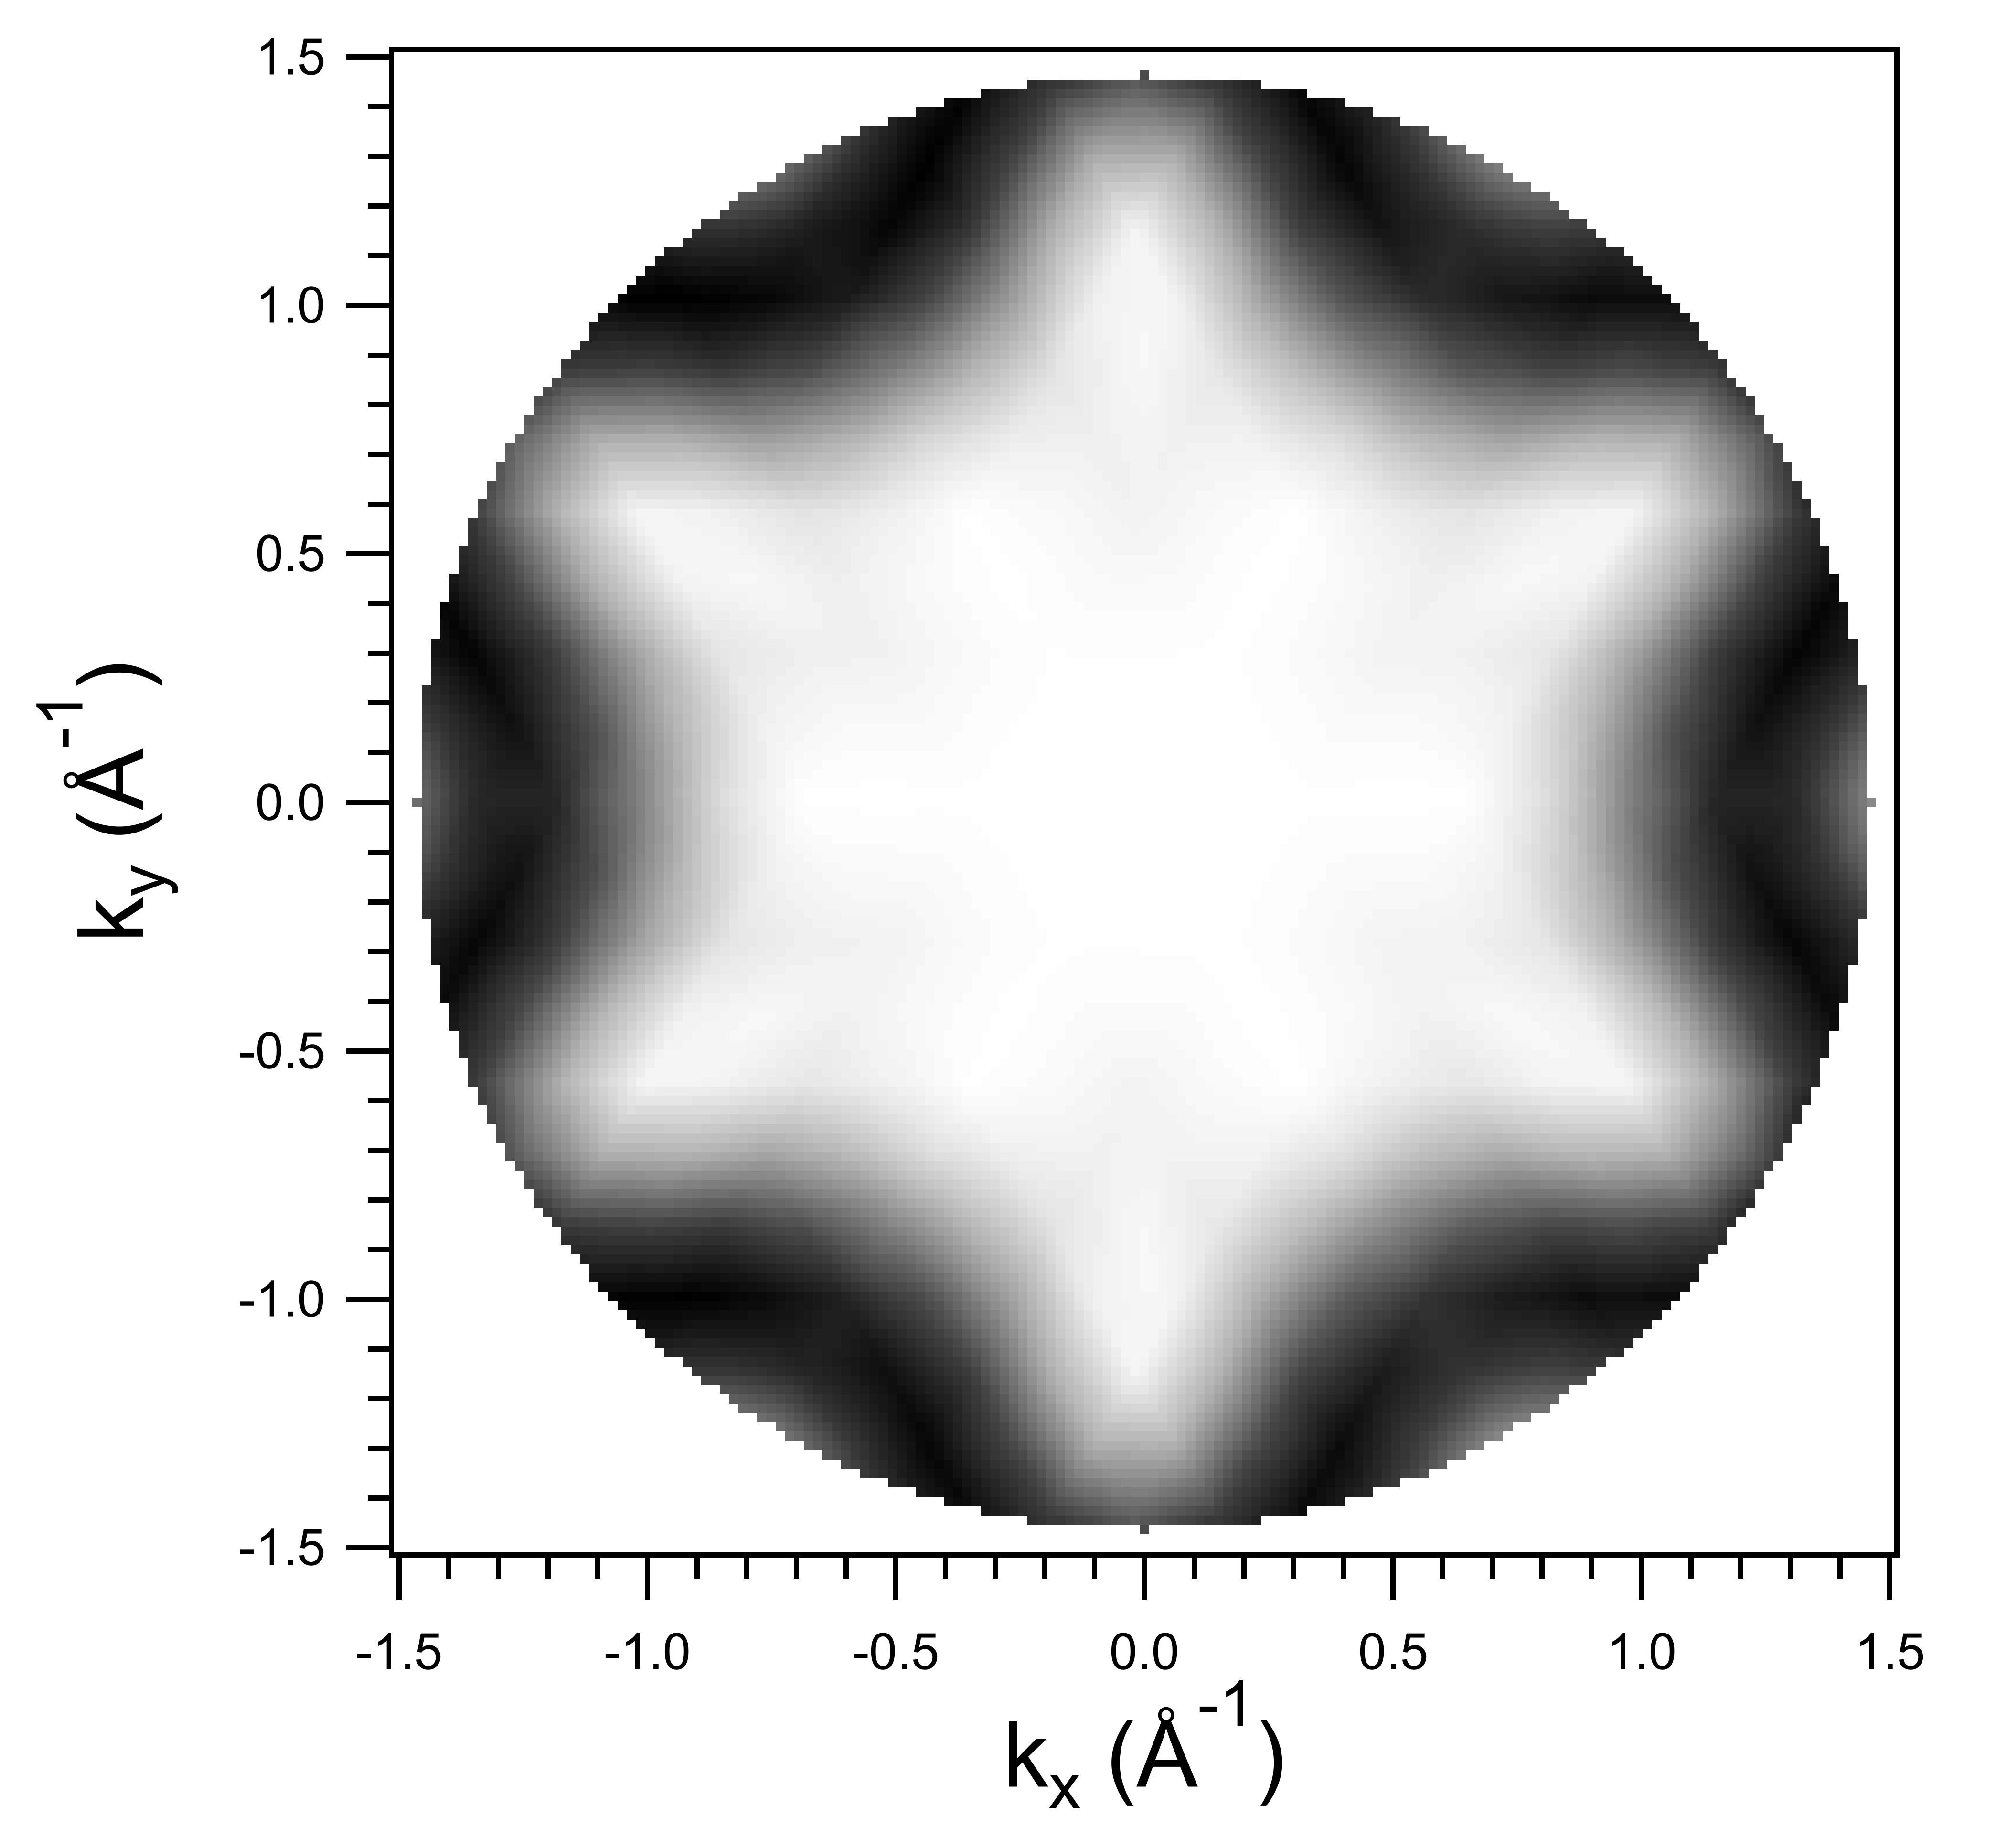
\includegraphics[height=5cm]{./content/pictures/Au+5A/HOMO1_all_CT}
                \subcaption{Theorie Oribtale mit Symmetrisierung zweimal um 120 Grad gedreht und zum Ursprungsbild addiert.}
                \label{fig:MOT_Au+5A_theo}
            \end{subfigure}
            \caption{Zuordnung eines Bildes zu einem der Molekülorbitale.}
            \label{fig:MOT_Au+5A}
        \end{figure}
        Winkelaufgelöste Bilder bei den entsprechenden Energien zeigen auch zusätzliche Merkmale im Bezug zum reinen Gold.
        Gemeinsam mit theoretischen Berechnungen aus der Dichtefunktionaltheorie lassen sich diese dann entsprechenden Molekülorbitalen zuordnen.
        Dies ist für einige Energien und Orbitale in \autoref{fig:MOT_Au+5A} geschehen.
        Dabei wurden die gemessenen wie auch berechneten Bilder entsprechend der Geometrie aus dem Beugungsbild \autoref{fig:LEED_Au+5A} jeweils um \SI{120}{\degree} gedreht und aufsummiert.
        Die theoretisch berechneten Bilder wurden mit Hilfe des Python Programms \textit{kmap.py} erstellt~\cite{brandstetter_kmappy_2021}.

        Eine Zuordnung einer der markanten Elemente zu einem zuvor unbestzten Orbital, dem LUMO ist nicht zu erkennen.
        Es scheint also so als würden keine Elektronen zwischen Substrat und Molekül ausgetauscht werden. 
        Dies lässt sich auch aus der Literatur erkennen, dass sich bei den Anornung von Pentacene auf Gold um den Prozess der Physisorption handelt~\cite{5A_4}.
        Abwesenheit des LUMOs in den Spektren und Bildern muss aber nicht zwangsläufig auf die Physisorption hindeuten.
        So ist Pentacene auf Kupfer (111) chemisch adsorbiert und zeigt dennoch keine Anzeichen der Besetzung des LUMO~\cite{koch_adsorption-induced_2008}.
        \begin{itemize}
            \item Peaks der Moleküle kennzeichnen
            \item Alle Molekülorbital zuordnungen vereinigen und ergänzen
            \item Bandstruktur deuten von Gold, Bänder zuordnen?
        \end{itemize}

        
    \section{Nickeloxid}    
        \begin{figure}
            \centering
            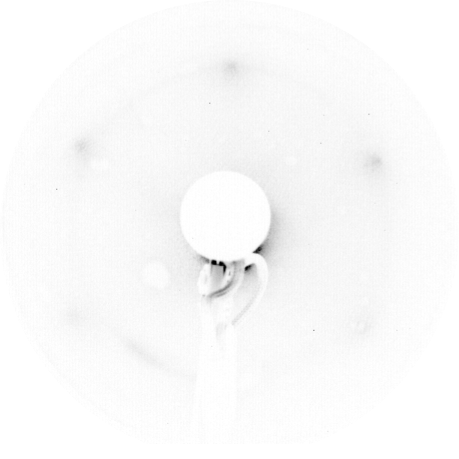
\includegraphics[height=5cm]{./content/pictures/NiO/2021_06_15_019_NiO(111)_73eV_Thicklayer}
            \caption{Der Nickeloxidfilm (111) bei einer Elektronenenergie von \SI{73}{\electronvolt}.}
            \label{fig:LEED_NiO}
        \end{figure}
        Auf die saubere Goldprobe wird bei Raumtemperatur ein Nickeloxidfilm aufgebracht.
        Dies geschieht durch das Aufdampfen von Nickel mit einer Rate von \SI{0.3}{\angstrom\per\minute} in einer Sauerstoffatmosphäre von \SI{2e-6}{\milli\bar}.
        Es ergibt sich dabei das LEED Bild in \autoref{fig:LEED_NiO}.
        Im Vergleich zu den klaren und scharfen Spots des sauberen Gold scheinen diese etwas ausgewaschen zu sein.
        Die Ursache daran liegt in der nicht ganz perfekten Oberflächenbeschaffenheit \cite{NiO_34}.
        Durch die polare Oberflächennatur der (111)-Orientierung und der damit verbundenen Instabilität können verschiedene Relaxationsprozesse auftreten \cite{NiO_36, NiO_35, NiO_34, NiO_27, NiO_10}.
        Die Positionen der Punkte hat sich bei dem Nickeloxidfilm im Vergleich zum Gold nicht wesentlich verändert, ihre Gitterkonstanten sind also nahezu gleich.
        Auch die Intensitäten der Reflexe beim Nickeloxid sind nun gleich groß für alle Punkte.
        Aus der gleichen Symmetrie der Spots und der Abwesenheit zusätzlicher Spots kann eine $\text{p}(2 \times 2)$ Rekonstruktion \cite{NiO_37} und Domänenbildung der (100)-Orientierung \cite{NiO_36} ausgeschlossen werden.
        Die hier wahrscheinlichste Stabilisierung der Oberfläche ist die \ce{OH-}-Terminierung mit der $\text{p}(1 \times 1)$-Rekonstruktion \cite{NiO_35}.
        Hierbei wird das Oberflächenpotential durch Reduzierung der Oberflächenladung verkleinert und die Oberfläche wird thermodynamisch stabil.

        \begin{figure}
            \centering
            \begin{subfigure}[t]{0.48\textwidth}
                \centering
                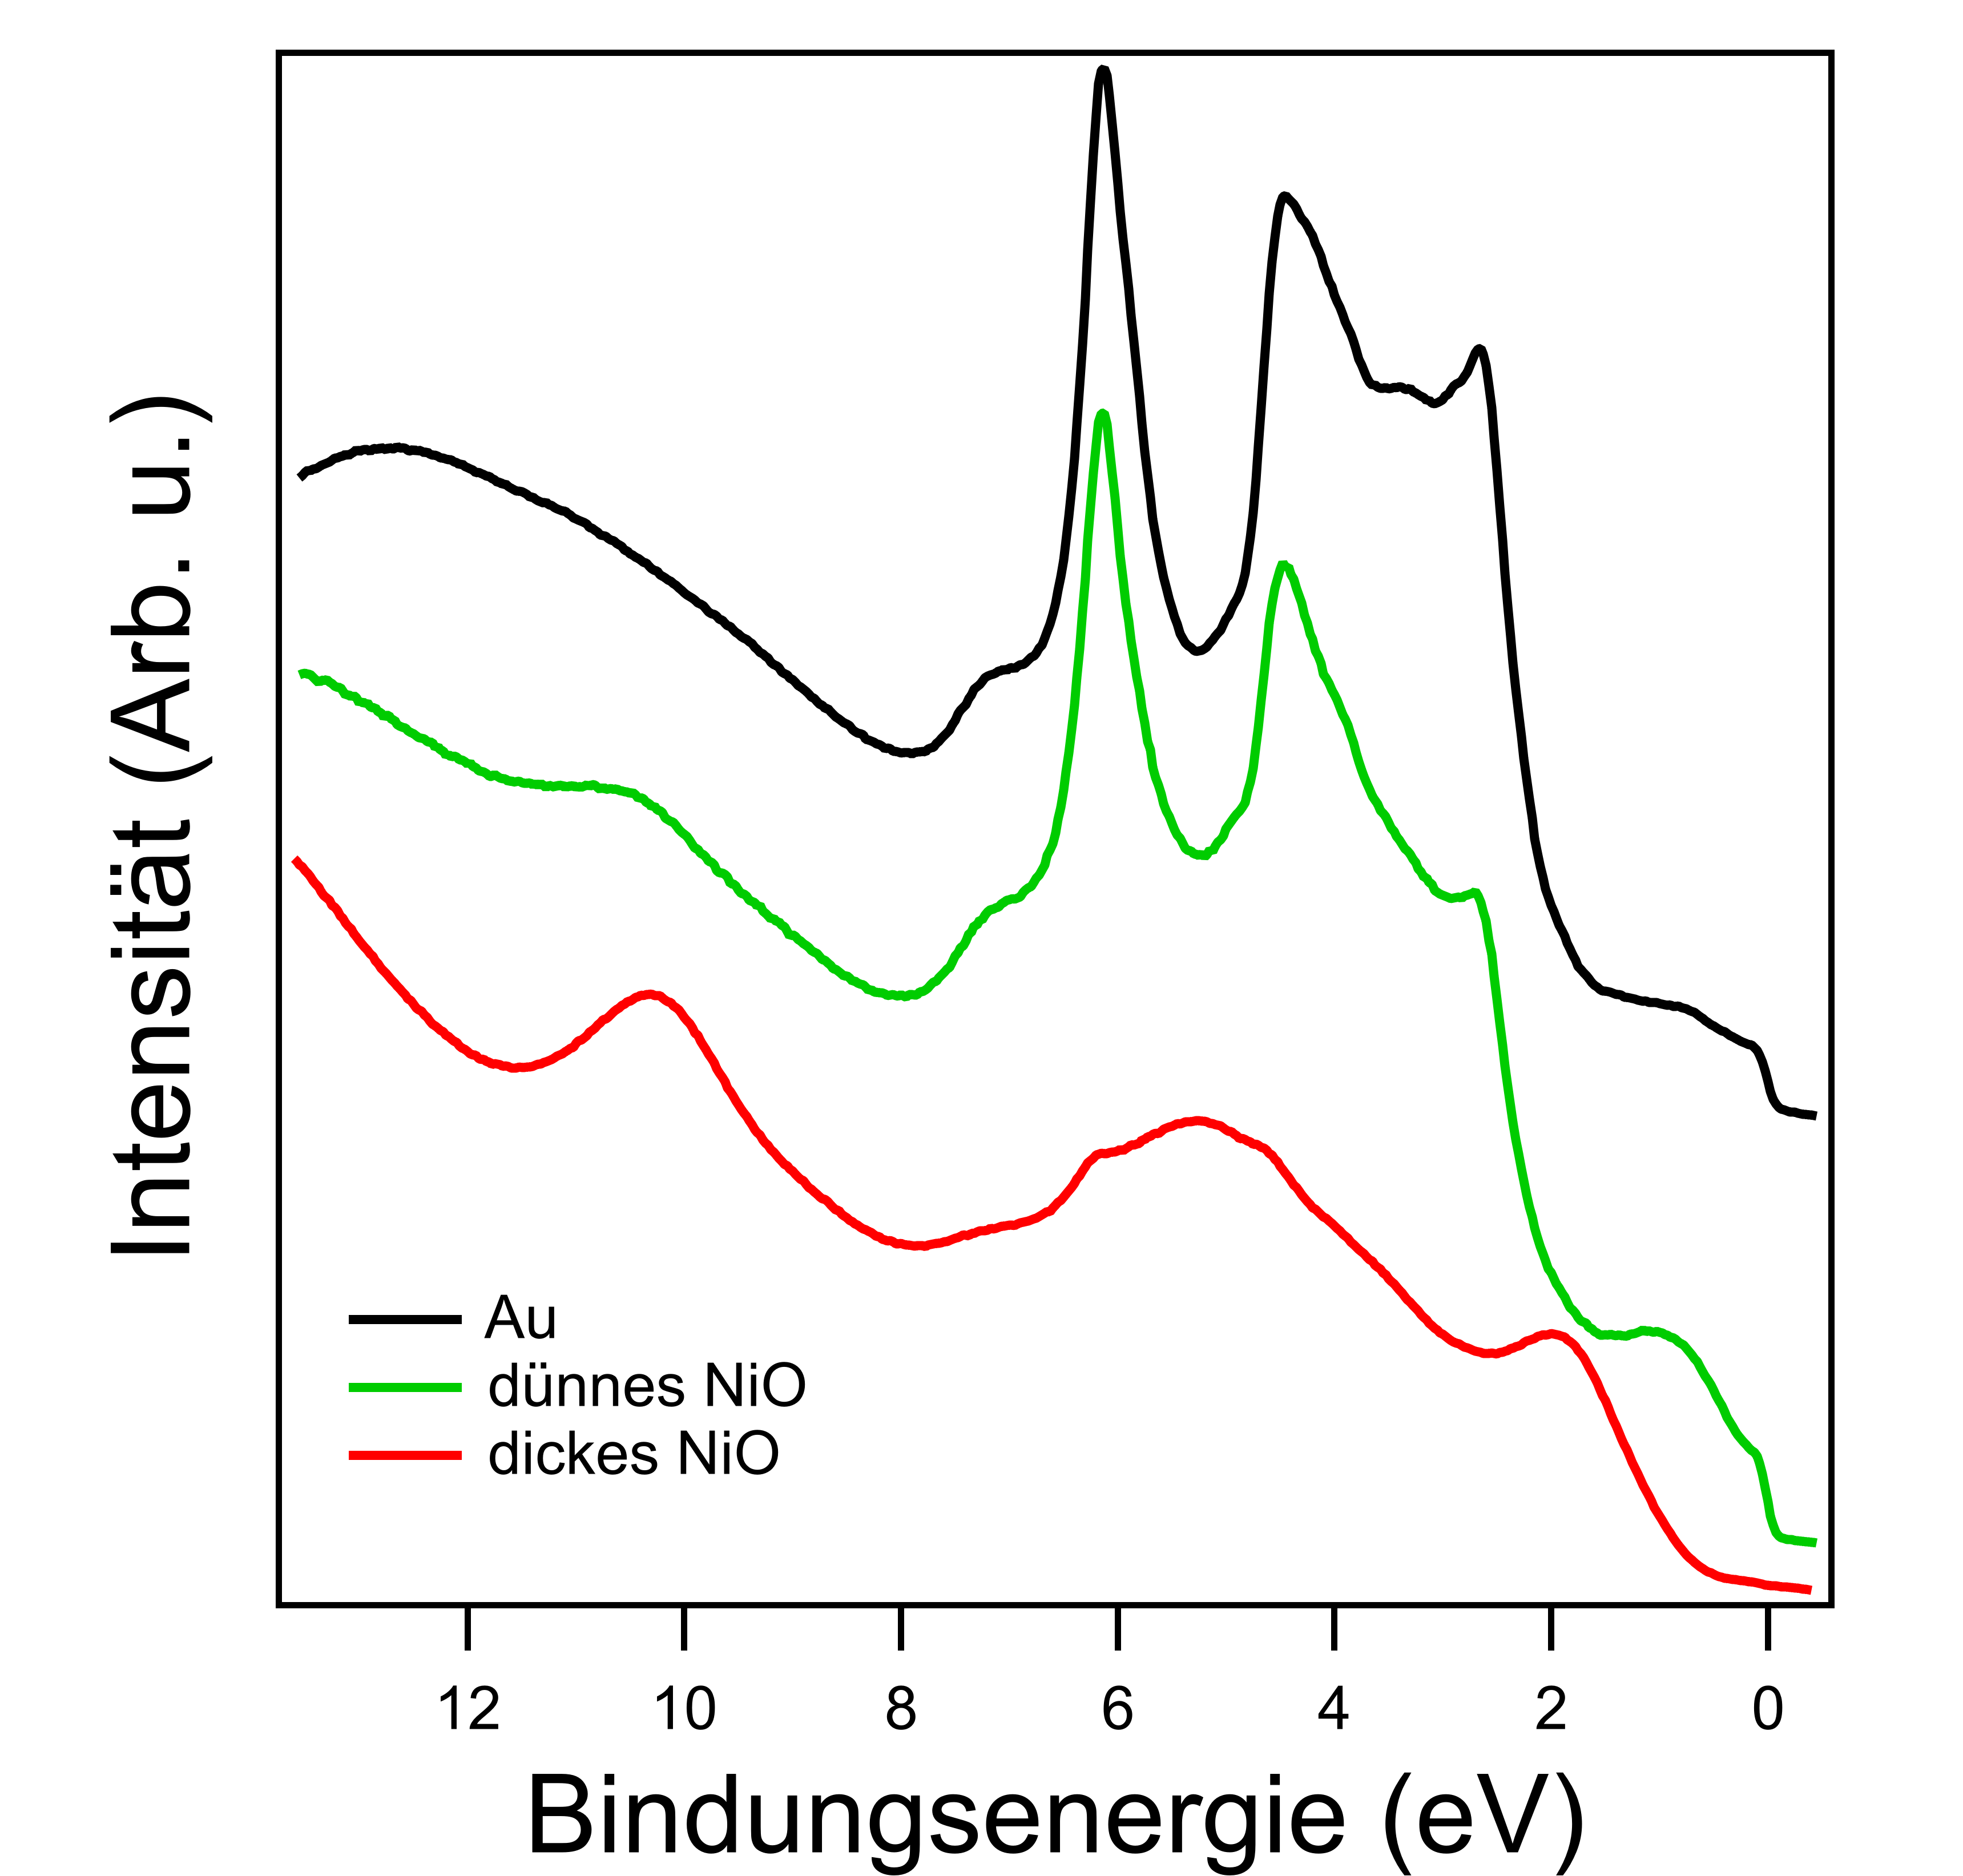
\includegraphics[height=5cm]{./content/pictures/NiO/NiO_Filmdicke.png}
                \subcaption{Die integrierten Spektren für zwei verschiedene Schichtdicken von \ce{NiO}. Als Referenz dient das integrierte Spektrum von Gold.}
                \label{fig:EDC_NiO}
            \end{subfigure}
            \begin{subfigure}[t]{0.48\textwidth}
                \centering
                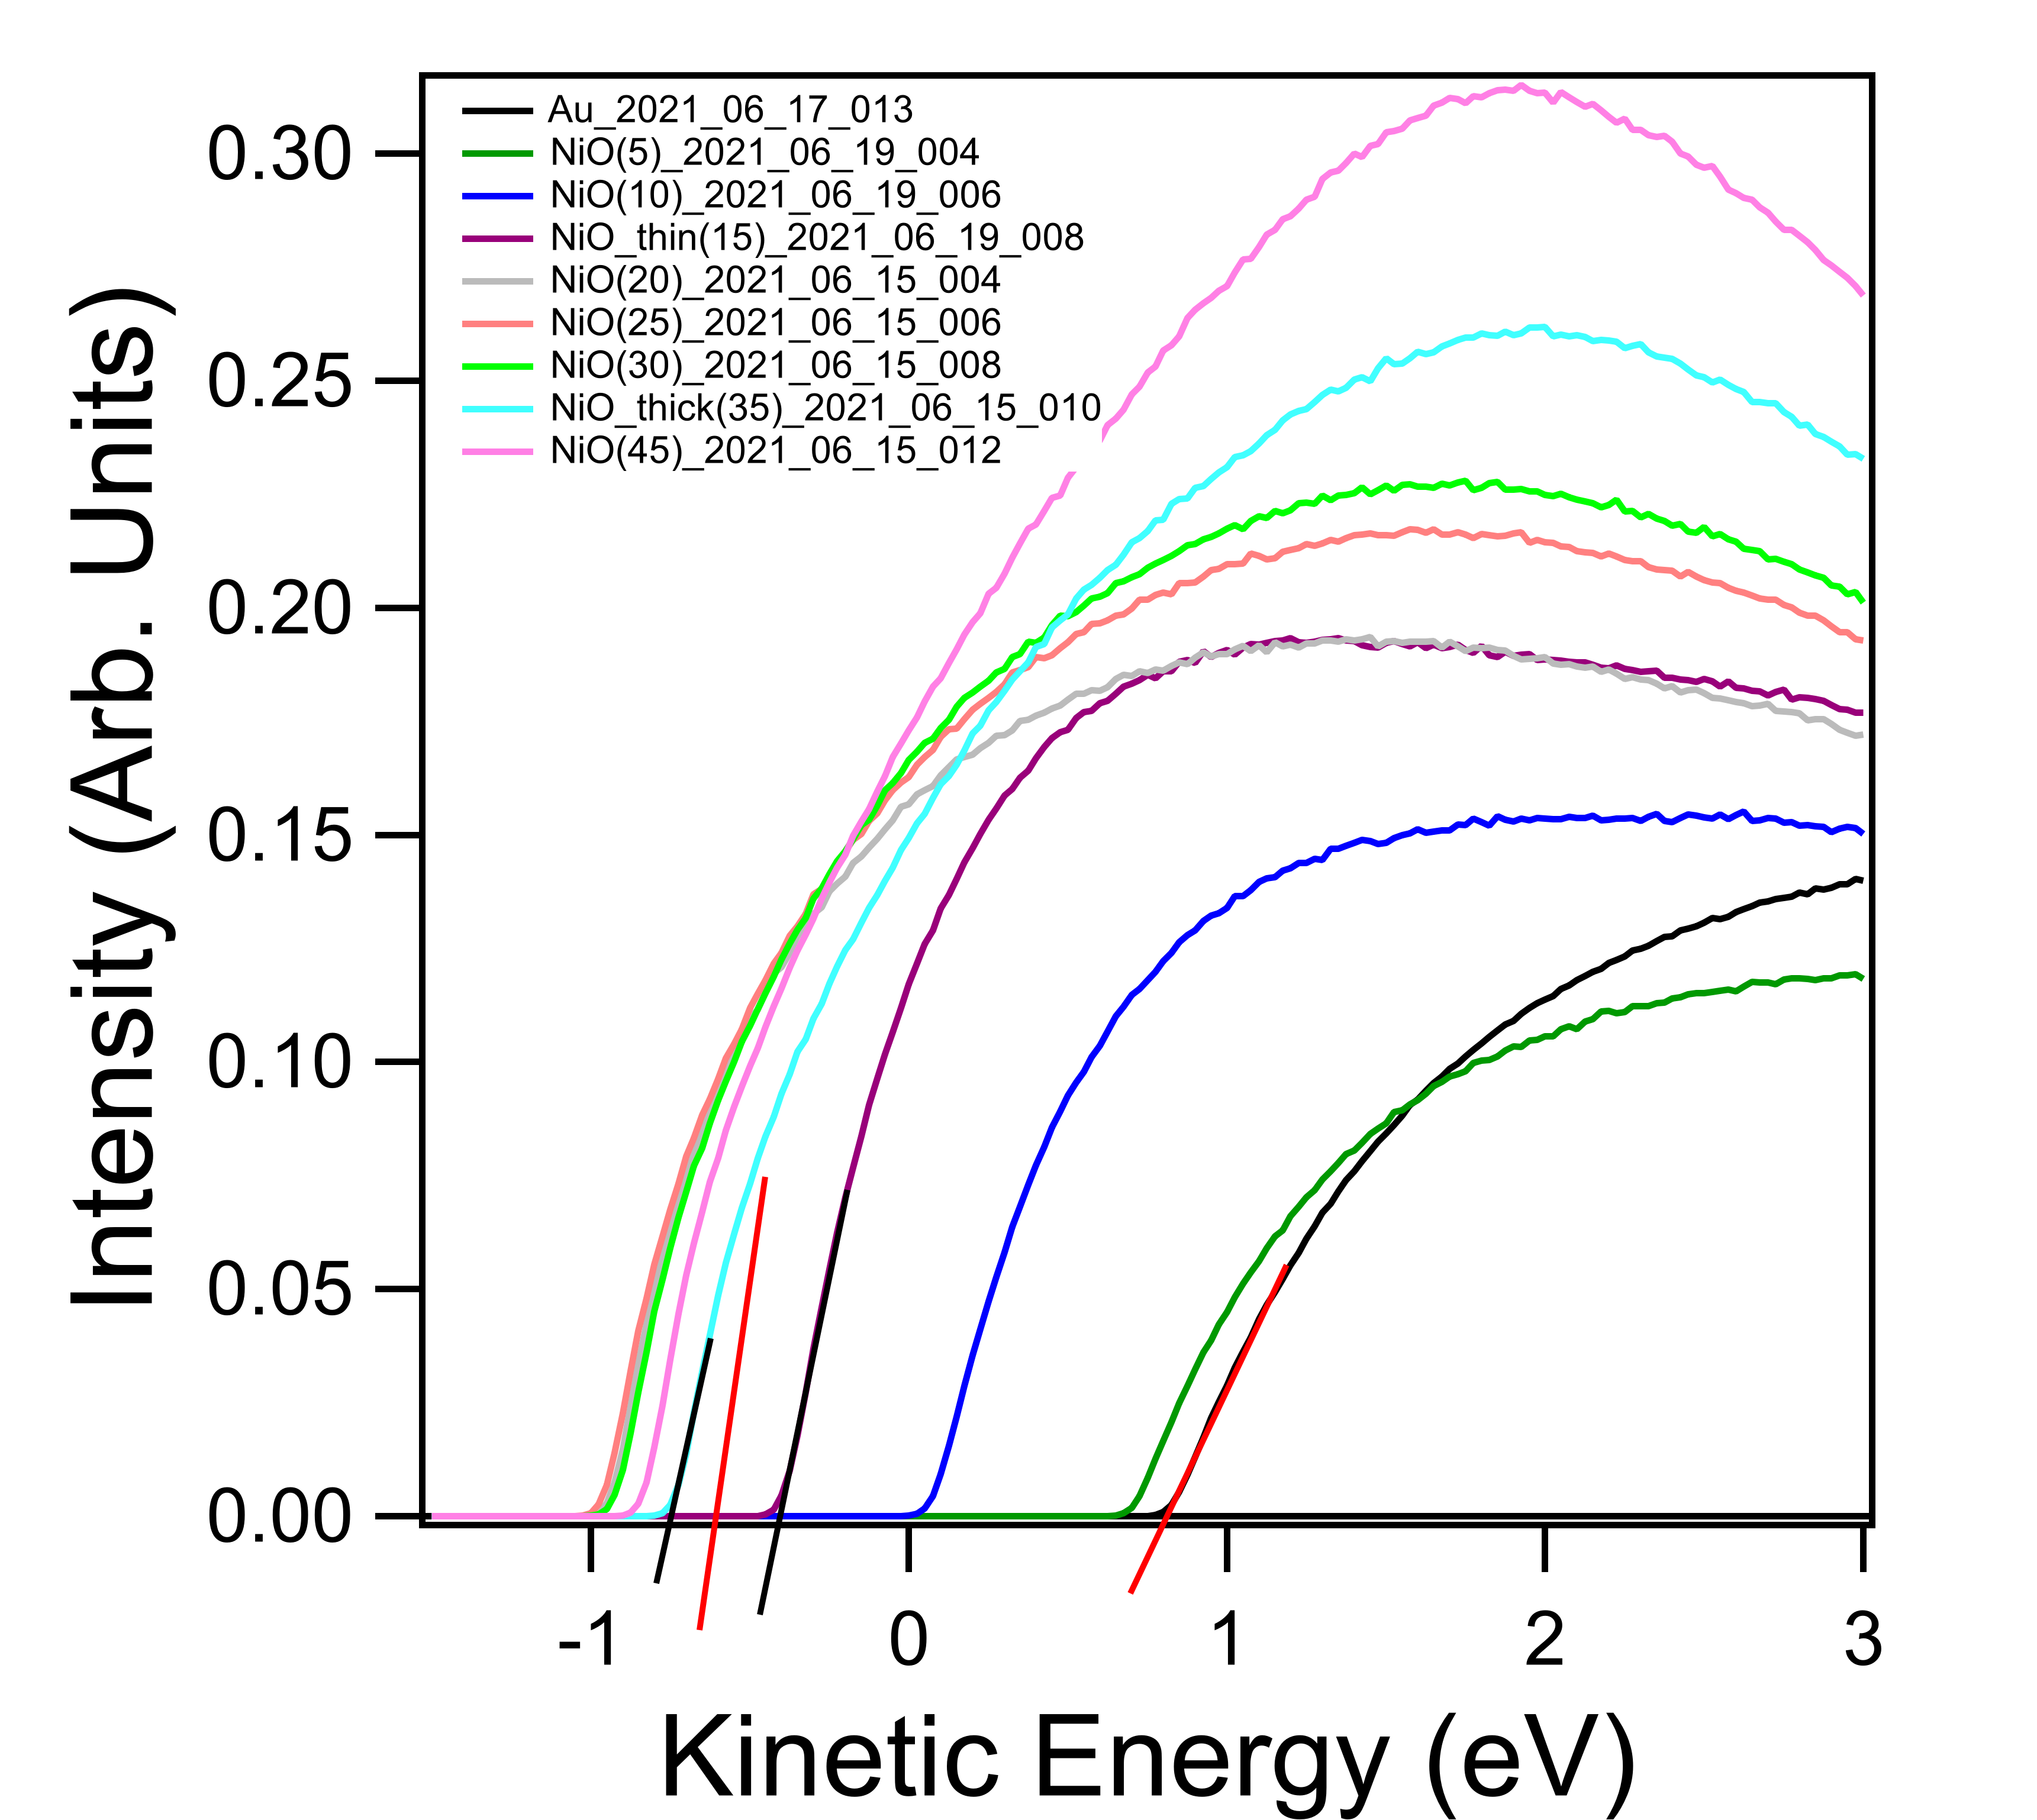
\includegraphics[height=5cm]{./content/pictures/NiO/NiO_WKF_thickness.png}
                \caption{Die integrierten Spektren im Bereich der Sekundärelektronen für verschiedene Schichtdicken von \ce{NiO}.}
                \label{fig:WKF_NiO}
            \end{subfigure}
            \caption{Integrierte Spektren für verschidene Schichtdicken und Bereiche des Nickeloxidfilms.}
        \end{figure}
        
        Durch Variation der Aufdampfzeiten lassen sich verschiedene Schichtdicken von Nickeloxidfilmen herstellen.
        Für zwei ausgewählte Zeiten sind die winkelintegrierten Spektren des Valenzbandbereiches in \autoref{fig:EDC_NiO} gemeinsam mit dem Spektrum des Substrates dargestellt.
        Zu erkennen ist, dass mit zunehmender Schichtdicke die charakteristischen Merkmale des Substrates abnehmen.
        Dafür steigt das Signal, was vom Nickeloxid herrührt an.
        Erkennbar ist somit auch die Oberflächenemfindlichkeit, der verwendeten Methode, da tiefer Lagen nur noch gering zum Signal beitragen.
        Aus der Verschiebung des Punktes an dem die Sekundärelektronen aufhören lässt sich erkennen, dass sich die Austrittsarbeit vom Gold zu dickeren Filmen Nickeloxid zu kleineren Werten verschiebt.
        Dies ist auch in \autoref{fig:WKF_NiO} für verschiedene Aufdampfzeiten dargestellt. 
        Kleine Verschiebungen können durch unterschiedliche Aufdampfbedingungen erklärt werden, denn es ist bekannt das durch Variation der Parameter gezielt die Eigenschaften manipuliert werden können.
        Vom dünnen Nickeloxidfilm zum dickeren Nickeloxidfilm wechselt sie von \SI{4.25}{\electronvolt} zu \SI{3.90}{\electronvolt}.
        Die Austrittsarbeit des dicken Nickeloxidfilms passt \textbf{oder passt nicht zu Quelle und Wert}.

        \begin{figure}
            \centering
            \begin{subfigure}[t]{0.48\textwidth}
                \centering
                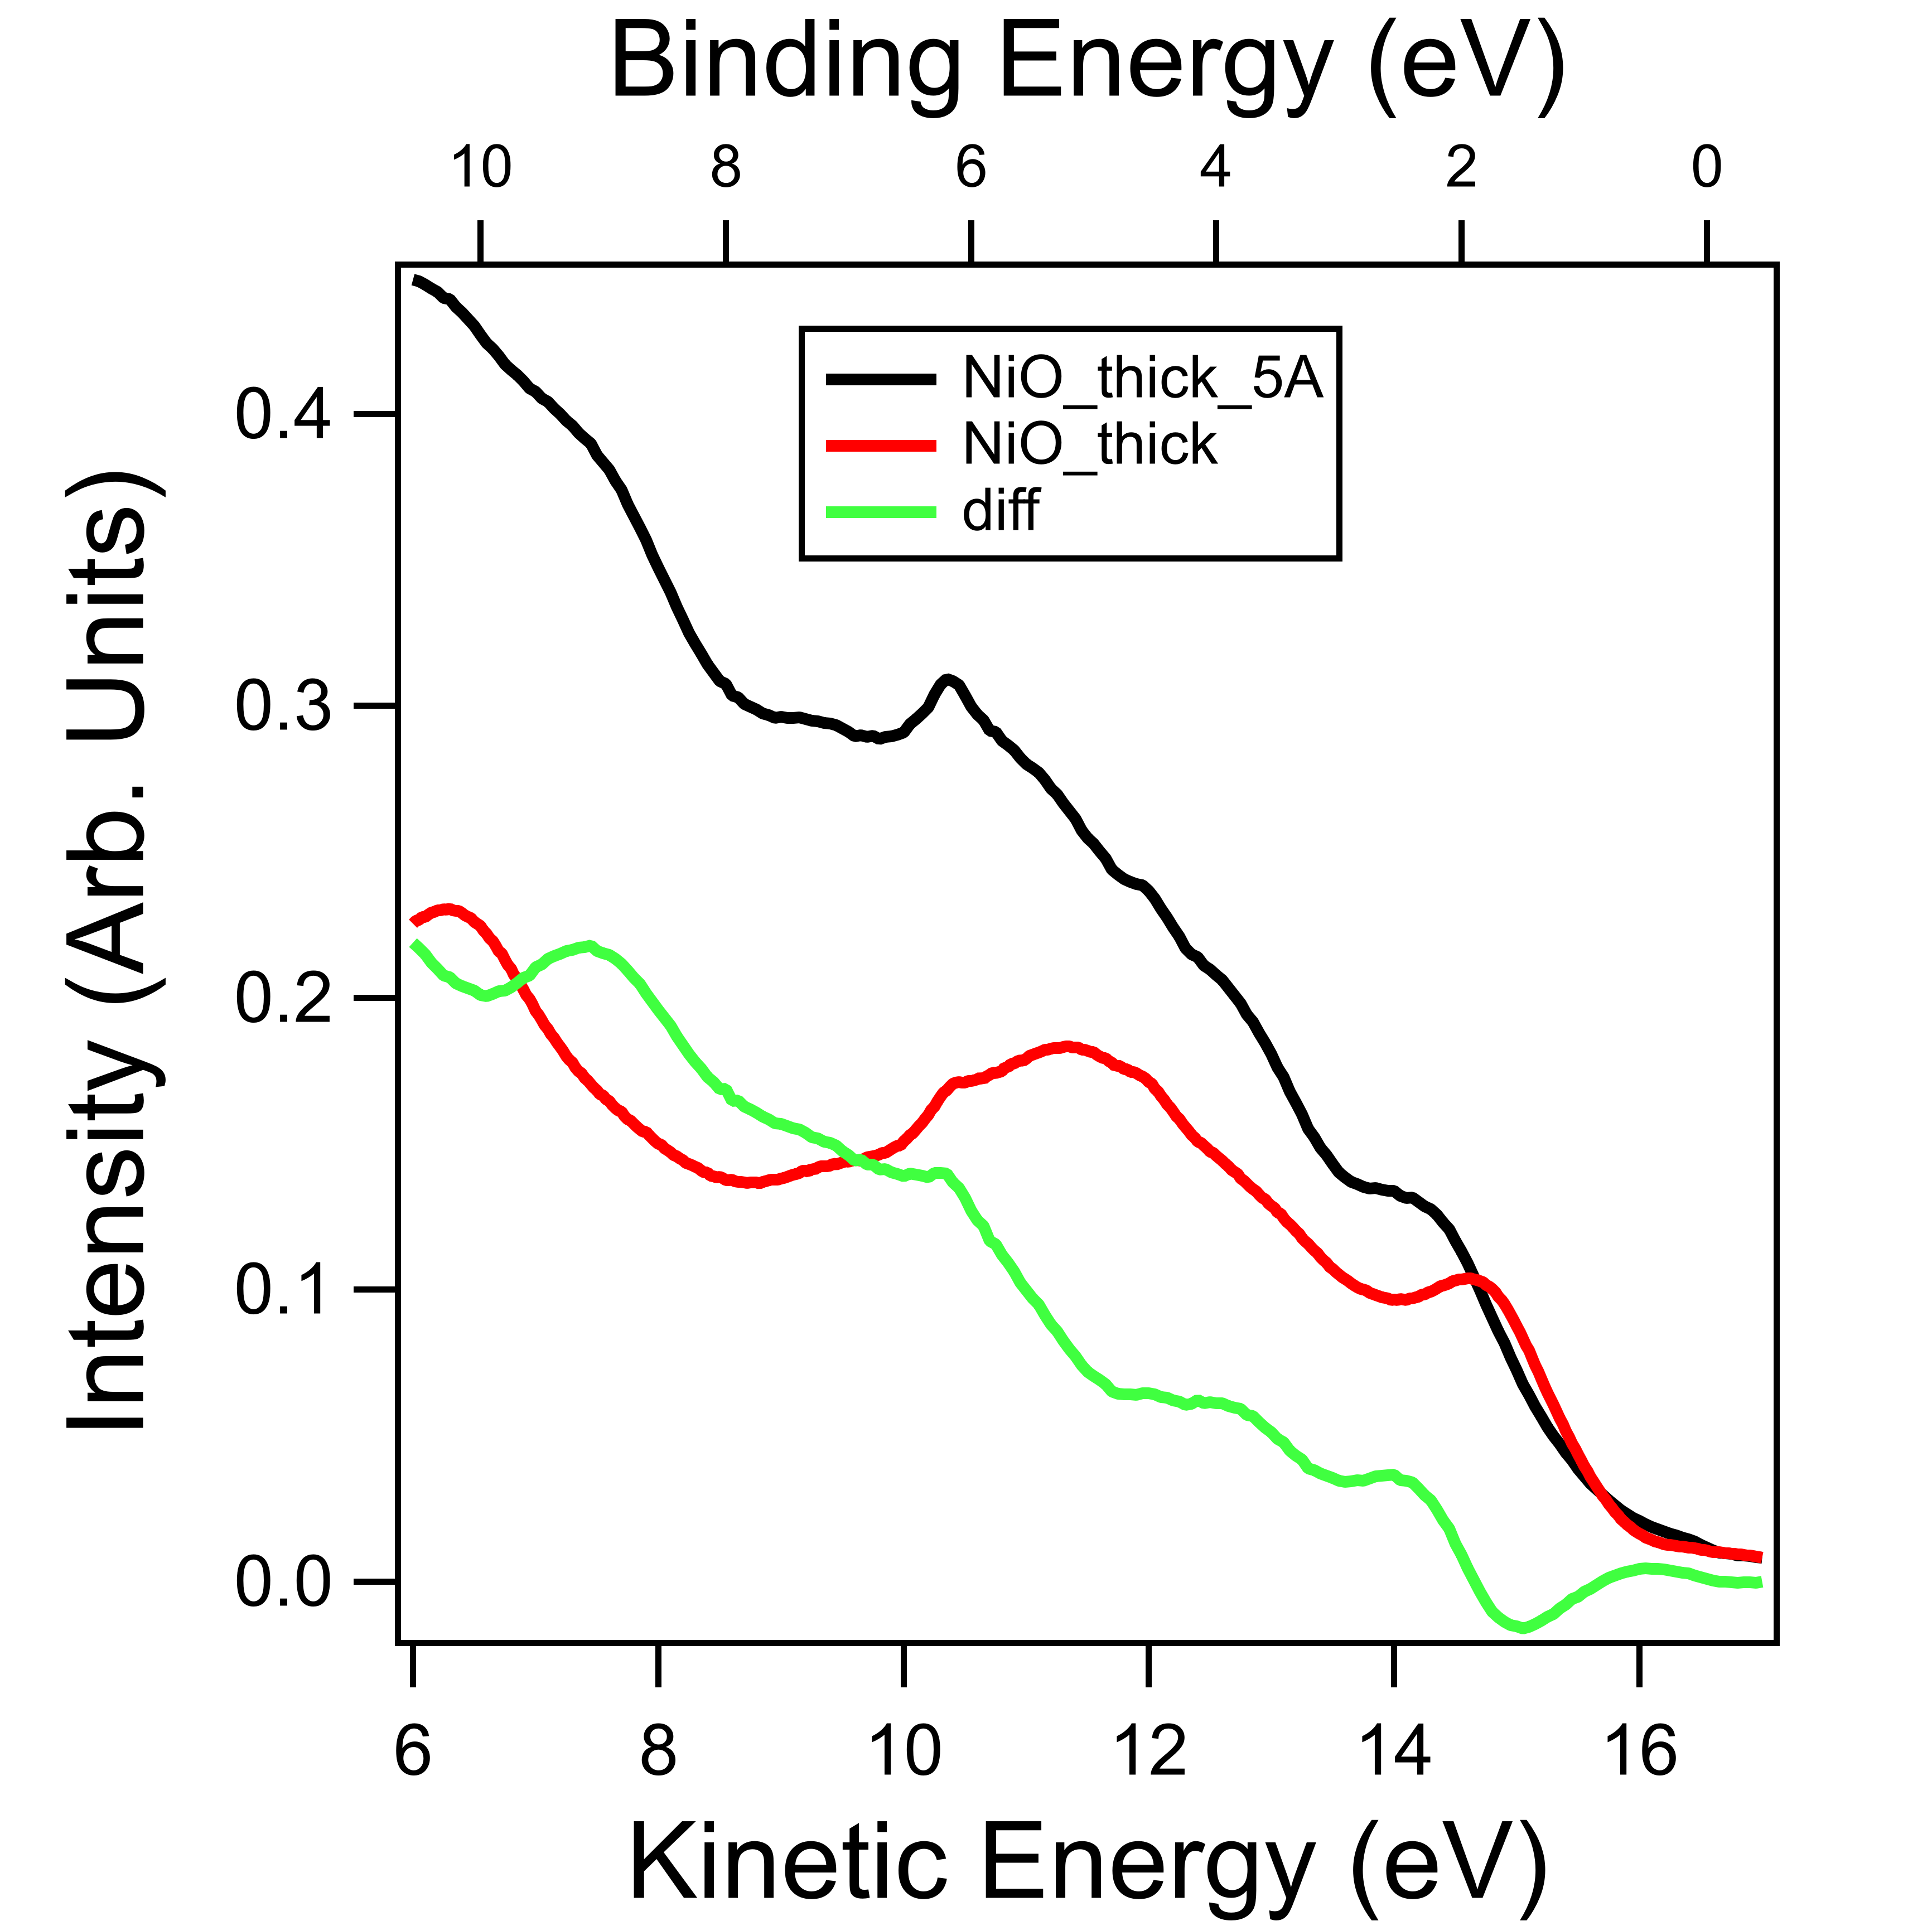
\includegraphics[height=5cm]{./content/pictures/NiO+5A/NiO_thick_5A.png}
                \subcaption{Die integrierten Spektren für einen dicken Nickeloxidfilm, mit zusaätzlich einer Monolage Pentacene und deren Differenz.}
                \label{fig:EDC_NiO+5A}
            \end{subfigure}
            \begin{subfigure}[t]{0.48\textwidth}
                \centering
                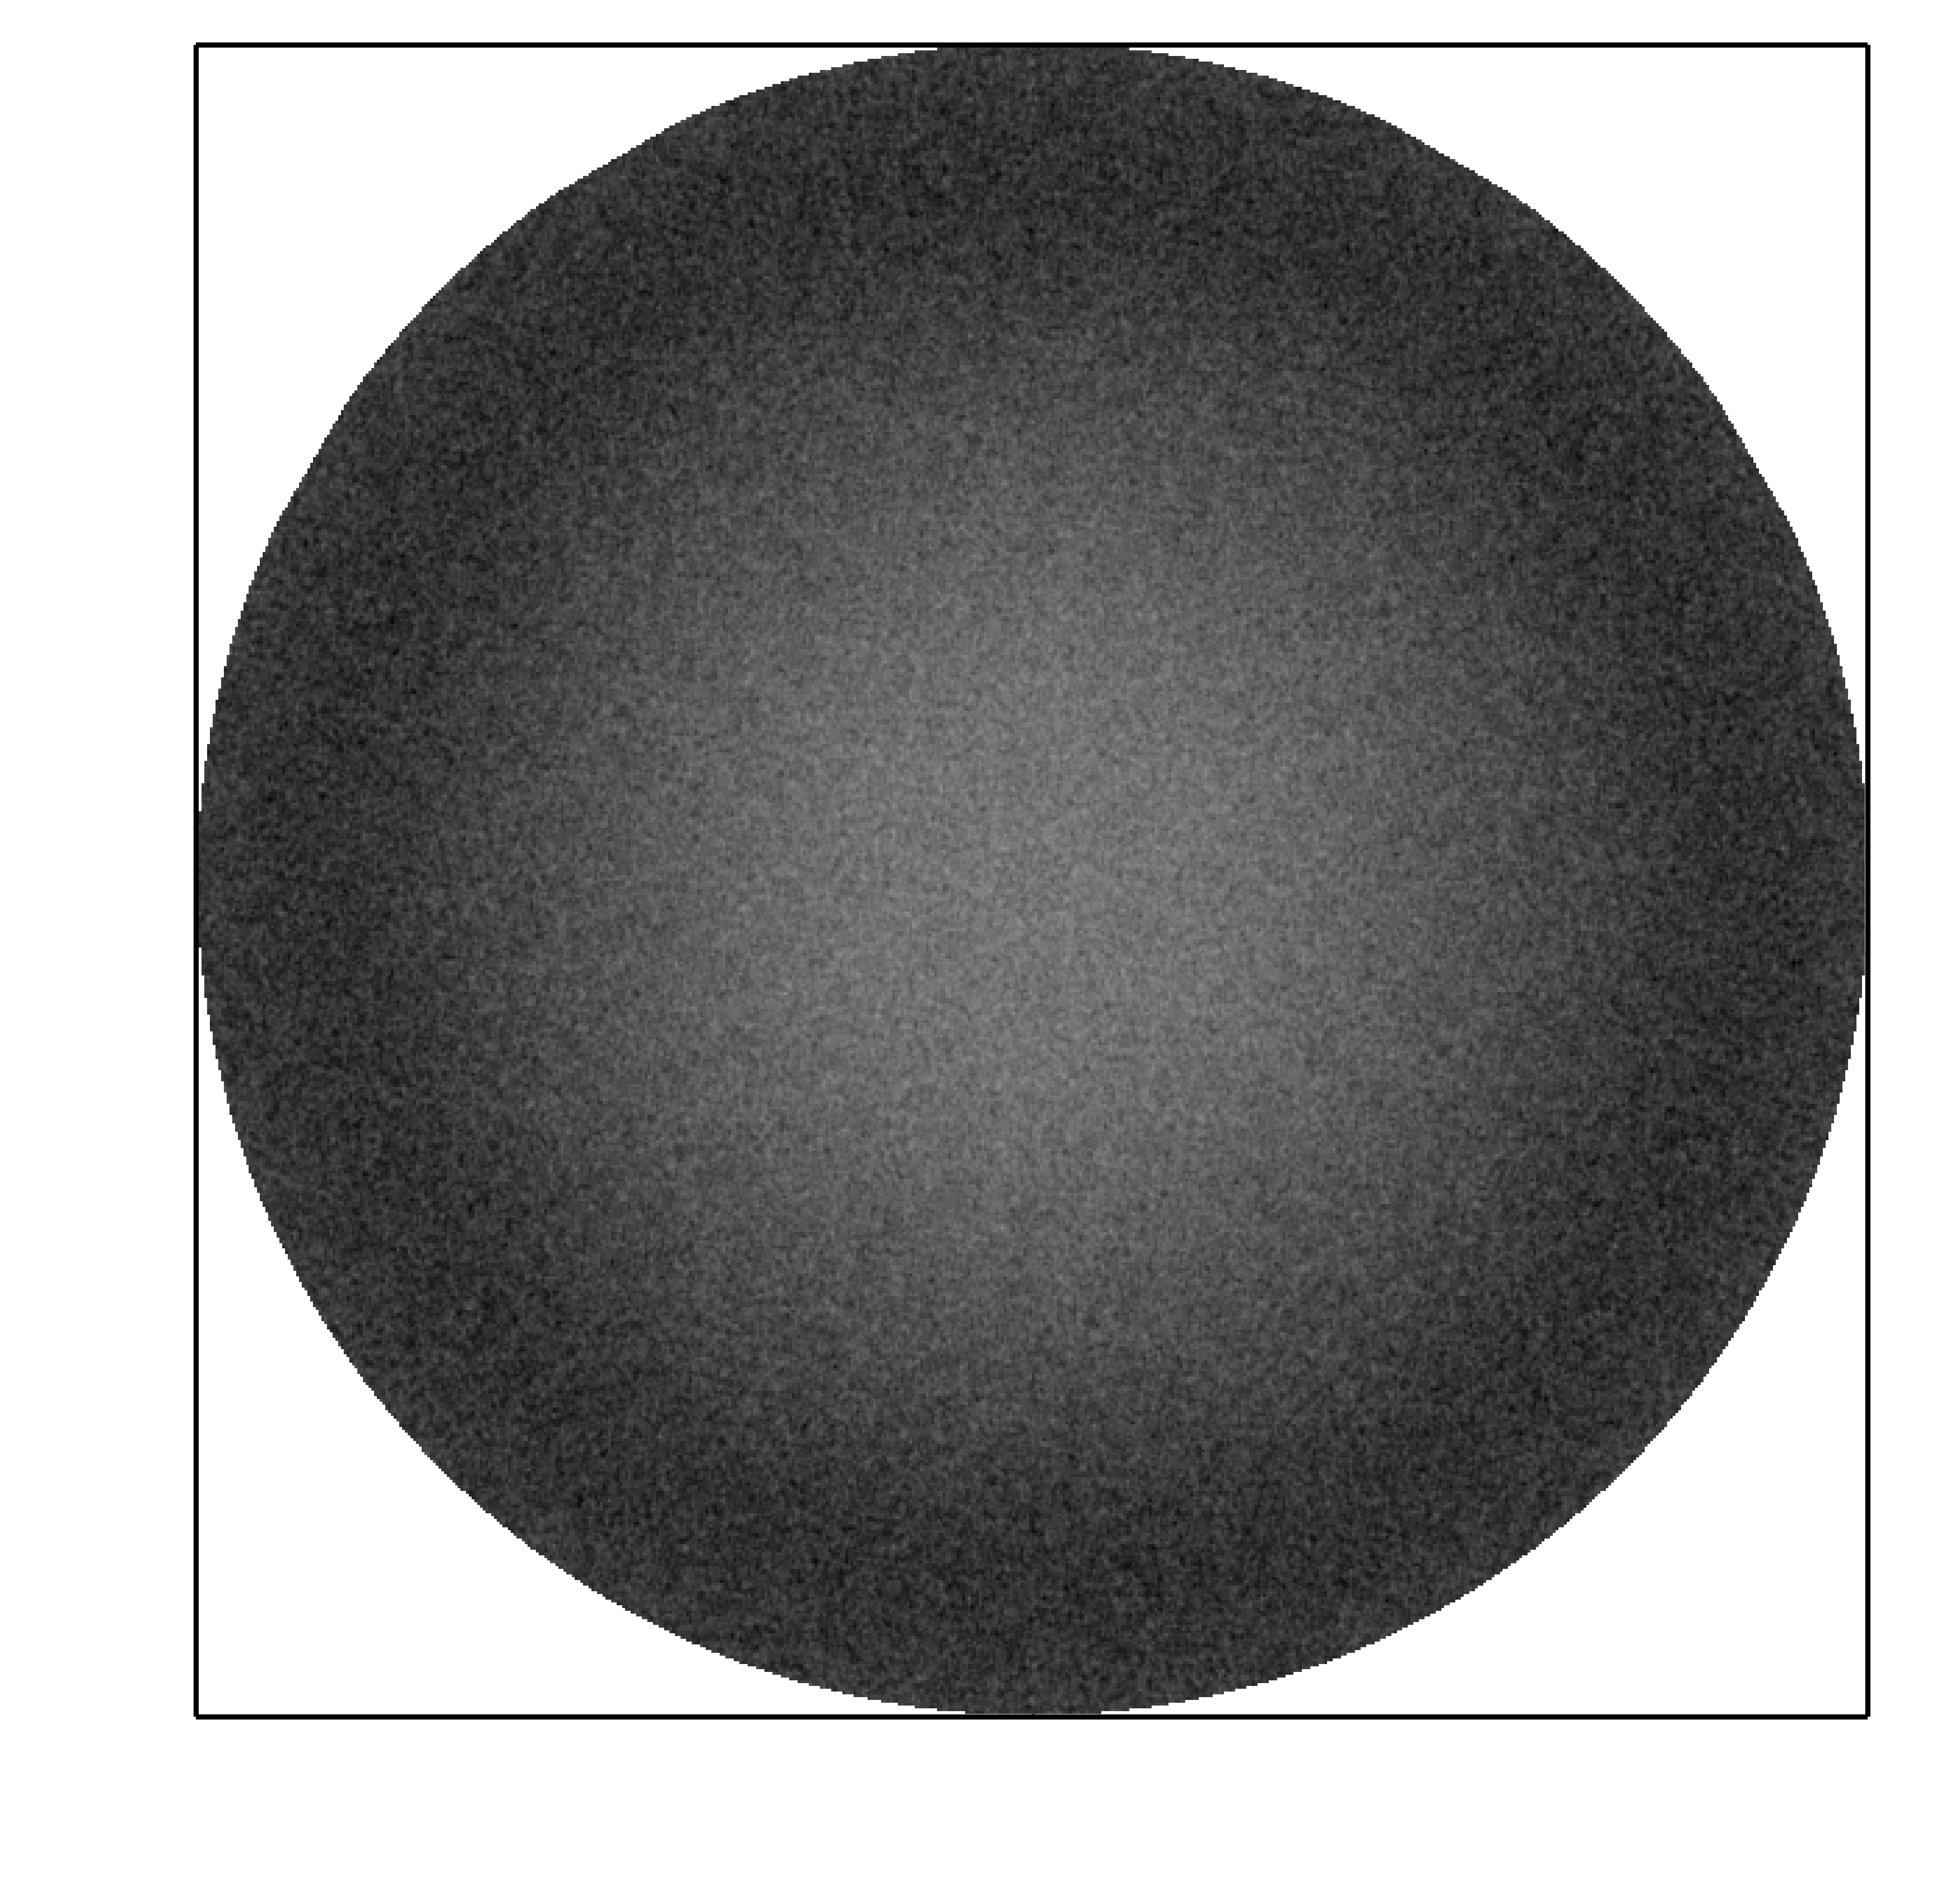
\includegraphics[height=5cm]{./content/pictures/NiO+5A/NiO_thick_5A_KE12_7.png}
                \subcaption{Map für Pentacene auf dicken Nickeloxidfilm bei einer kinetischen Energie von \SI{7.5}{\electronvolt}. Also Bindungsenergie von \SI{3.85}{\electronvolt}.}
                \label{fig:NiO+5A}
            \end{subfigure}
            \caption{Integriertes Spektrum des Valenzband Bereiches für reines Nickeloxid und mit einer Monolage Pentacene, sowie ein winkelaufgelöstes Bild.}
        \end{figure}
        Das Aufdampfen von einer Monolage Pentacene brachte kein LEED-Bild mehr zu stande.
        Nach dem Aufdampfen wurde versucht LEED-Bilder aufzunehmen, es waren allerdings nur leichte Substratspots sichtbar.
        So lässt sich schlussfolgern, dass sich die Moleküle auf der Oberfläche nicht anordnen.
        Dabei zeigt der direkte Vergleich der integrierten Spektren in \autoref{fig:EDC_NiO+5A} des reinen Nickeloxid und das mit Pentacene drauf deutliche zusätzliche Spitzen.
        Die Abwesenheit sehr ausgeprägter Merkmale in den impulsaufgelösten Bildern bestätigt die Annahme, dass sich die Moleküle auf der Oberfläche nicht regelmäßig anordnen.
        Ferner überlappen dann die einzelnen Merkmale im Impulsraum, sodass ein ausgewaschenes Bild entsteht.
        Auch wenn sich in den integrierten Spektren in \autoref{fig:EDC_NiO} klar zeigt, dass sich bei einigen Energien die Intensität erhöht ist in den entsprechenden Bildern keine klare Zuordnung möglich.
        Ein Beispiel ist in \autoref{fig:NiO+5A} zu sehen, dieses Bild wurde gewählt da ein deutliches Signal im integrierten Spektrum zu erkennen ist und die entsprechende Energie nicht zu weit weg von der Fermikante liegt.
        tendenziell sollten entsprechend winkelaufgelöste Bilder den theoretischen Berechnungen wie in \autoref{fig:MOT_Au+5A_theo} entsprechen, da Substrate gleiche Symmetrien aufweisen.
        \begin{itemize}
            \item WKF Shift für dicken
            \item NiO-Spektrum Peaks zuordnen
            \item linear ansteigender Untergrund bei Molekülen ? zu sehen in der Differenz
        \end{itemize}


    \section{Eisen}
        \begin{figure}
            \centering
            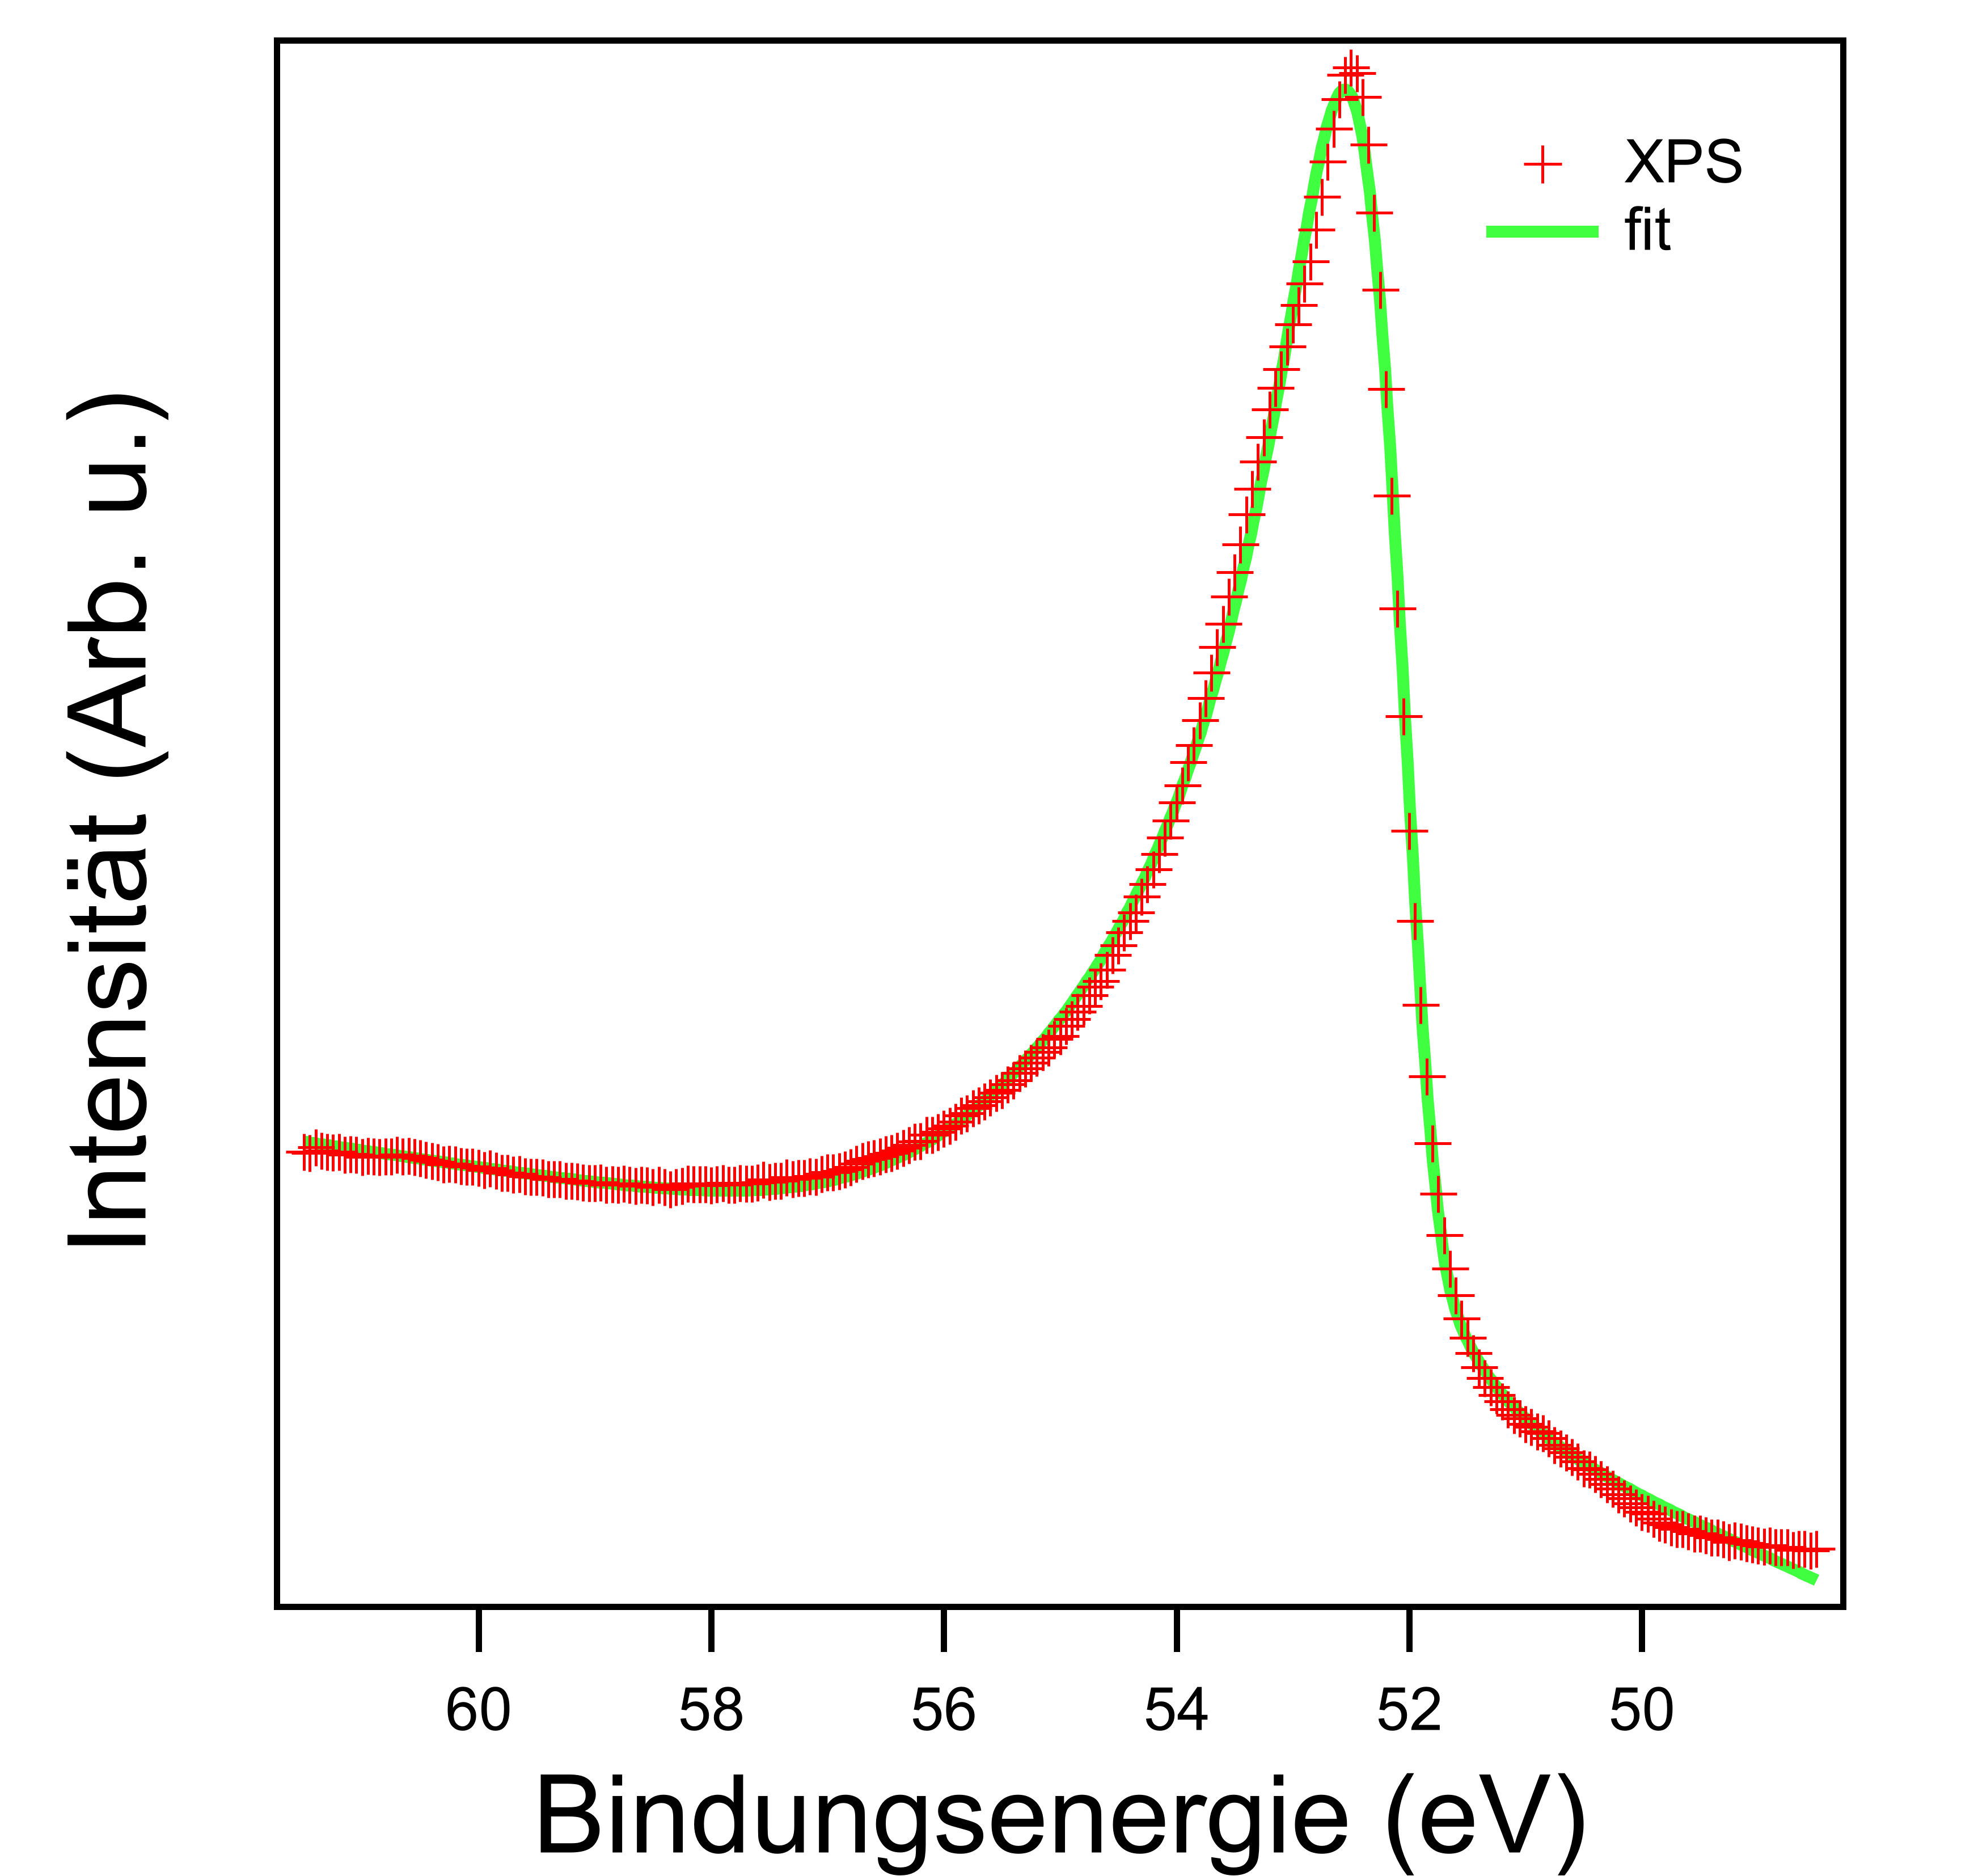
\includegraphics[width=0.5\textwidth]{./content/pictures/Fe/Fe3p_Fe.png}
            \caption{XPS Spektrum des $\ce{Fe}_{3\text{p}}$ Übergang des reinen Eisens. Hier passt der Fit mit einem Voigt (+Tougaard) sehr gut!}
            \label{fig:XPSFe3p_Fe}
        \end{figure}
        \begin{figure}
            \centering
            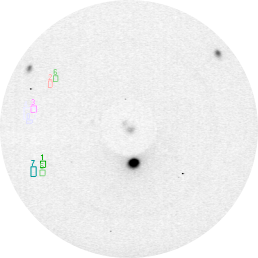
\includegraphics[height=5cm]{./content/pictures/pFe/2021_09_07_001_passivatedFe(100)_44eV.png}
            \caption{Passiviertes Eisen (100) bei einer Elektronenenergie von \SI{44}{\electronvolt}.}
            \label{fig:LEED_pFe}
        \end{figure}
        Bei der verwendeten Eisenprobe handelt es sich um einen dünnen Eisenfilm, der auf einem Magnesiumoxid Substrat gewachsen wurde.
        Die Probe wurde ebenfalls durch leichtes ioneninduziertes Zerstäuben und aufheizen auf \SI{600}{\celsius} gerreinigt.
        Die Reinheit der Probe lässt sich auch am Spektrum des $\ce{Fe}_{3\text{p}}$ Übergangs in \autoref{fig:XPSFe3p_Fe} erkennen.
        Das Signal bei \SI{52.83}{\electronvolt} lässt sich nach Abzug eines Pseudo-Tougaard Untergrund sehr gut mit einer Pseudo-Voigt Funktion approximieren.
        Entsprechend gab sich die Halbwertsbreite zu \SI{2.11}{\electronvolt}.
        Um Verunreinigungen des sehr reaktiven sauberen Eisens zu vermeiden, wird die Probe anschließend direkt passiviert.
        Dies geschieht in einer Sauerstoffatmosphäre von \SI{1.3e-7}{\milli\bar} für fünf Minuten, während die Probe bei \SI{550}{\celsius} gehalten wird.
        Die Probe wird dann nocheinmal kurz auf \SI{600}{\celsius} aufgeheizt.
        Nun wird auch dessen Oberflächenbeschaffenheit kontrolliert und entsprechendes LEED-Bild ist in \autoref{fig:LEED_pFe} zu sehen.
        Sie Spots sind scharf und zeigen auch die Geometrie der $\ce{Fe}-\text{p}(1 \times 1)\ce{O}$ Struktur.
        Die gesamten Spots sind dabei nicht zentrosymmetrisch, da die Probe verkippt ist, wodurch auch der (0,0)-Reflex zu sehen ist.

        Um ebefalls die kinetische Energie in die übliche Bindungsenergie umzurechnen muss die Austrittsrabeit des Analysators bestimmt werden.
        Dies ist nötig, da es sich bei den Eisenmonooxid um einen Isolator handelt und hier also die Fermikante nicht ermittelt werden kann.
        Aus der Anpassung an der Fermikante des Eisens lässt sich dessen Position auf \SI{59.5}{\electronvolt} bei einer Photonenenergie von \SI{64}{\electronvolt} bestimmen.
        Dadurch lässt sich für die spätere Umrechnung in die Bindungsenergie die Austrittsarbeit des Analysators bei NanoESCA auf \SI{4.5}{\electronvolt} festlegen.
        Anzumerken ist, dass die Genauigkeit dieser Annahme nicht exakt ist, da zusätzlich die Fermikante durch ein starkes Signal überlagert wird.
        Aus dem Abschnitt der Sekundärelektronen lässt sich ferner dann die Austrittsarbeit der Eisenprobe auf \SI{4.06}{\electronvolt} bestimmen.
        \begin{figure}
            \centering
            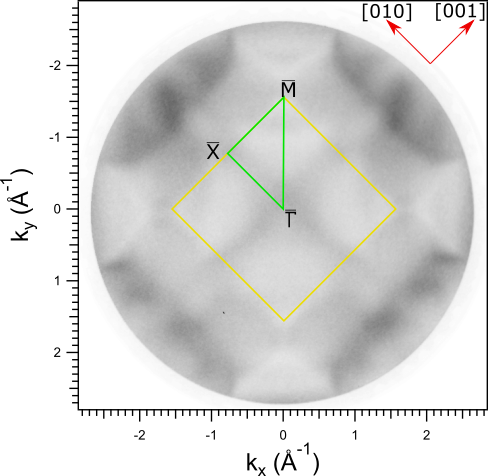
\includegraphics[width=0.5\textwidth]{./content/pictures/Fe/BZ_Fe.png}
            \caption{Die Brillouinzone des reinen Eisens bei einer Bindungsenergie von \SI{0.3}{\electronvolt}.
            Eigezeichnet sind auch die Vektoren, sowie einige Hochsymmetrierichtungen.
            Die Kantenlänge der BZ ist $\frac{2\pi}{a} = \SI[per-mode=reciprocal]{2.20}{\per\angstrom}$.
            Im Zentrum liegt der $\overline{\Gamma}$-Punkt, der Abstand zum $\overline{X}$-Punkt ist $\frac{2\pi}{2 \cdot a} = \SI[per-mode=reciprocal]{1.10}{\per\angstrom}$ und zum $\overline{M}$-Punkt $\frac{2\pi}{2 \cdot a} \sqrt{2} = \SI[per-mode=reciprocal]{1.55}{\per\angstrom}$.}
            \label{fig:BZ_Fe}
        \end{figure}
        Wie schon für das Gold lässt sich auch die Oberflächenbrillouinzone des Eisens darstellen. 
        Dies ist in \autoref{fig:BZ_Fe} geschehen.
        Aus ihr lässt sich dann anschließend wieder die Bandstruktur extrahieren.
        

    \section{Magnetit}
        \begin{figure}
            \centering
            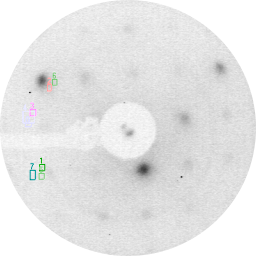
\includegraphics[height=5cm]{./content/pictures/Fe3O4/2021_09_07_012_FeO(100)_44eV.png}
            \caption{\ce{Fe3O4} (100) bei einer Elektronenenergie von \SI{44}{\electronvolt}.}
            \label{fig:LEED_Fe3O4}
        \end{figure}
        Auf dem der passivierten Eisenoberfläche wird Eisen mit einer Rate von \SI{0.6}{\ML\per\minute} und einem Sauerstoffdruck von \SI{2e-7}{\milli\bar} aufgedampft.
        Dabei wird die Probe auf eine Temperatur von \SI{230}{\celsius} gehalten.
        Zum abschluss wird die Temperatur auf \SI{600}{\degree} für fünf Minuten erhöht.
        So ergibt sich in \autoref{fig:LEED_Fe3O4} das Beugungsbild der Oberfläche.
        Es sind klar deutlich mehr Spots zu erkennen, die auf eine $\text{p}(1 \times 1)$-Überstruktur hindeuten.

        \begin{figure}
            \centering
            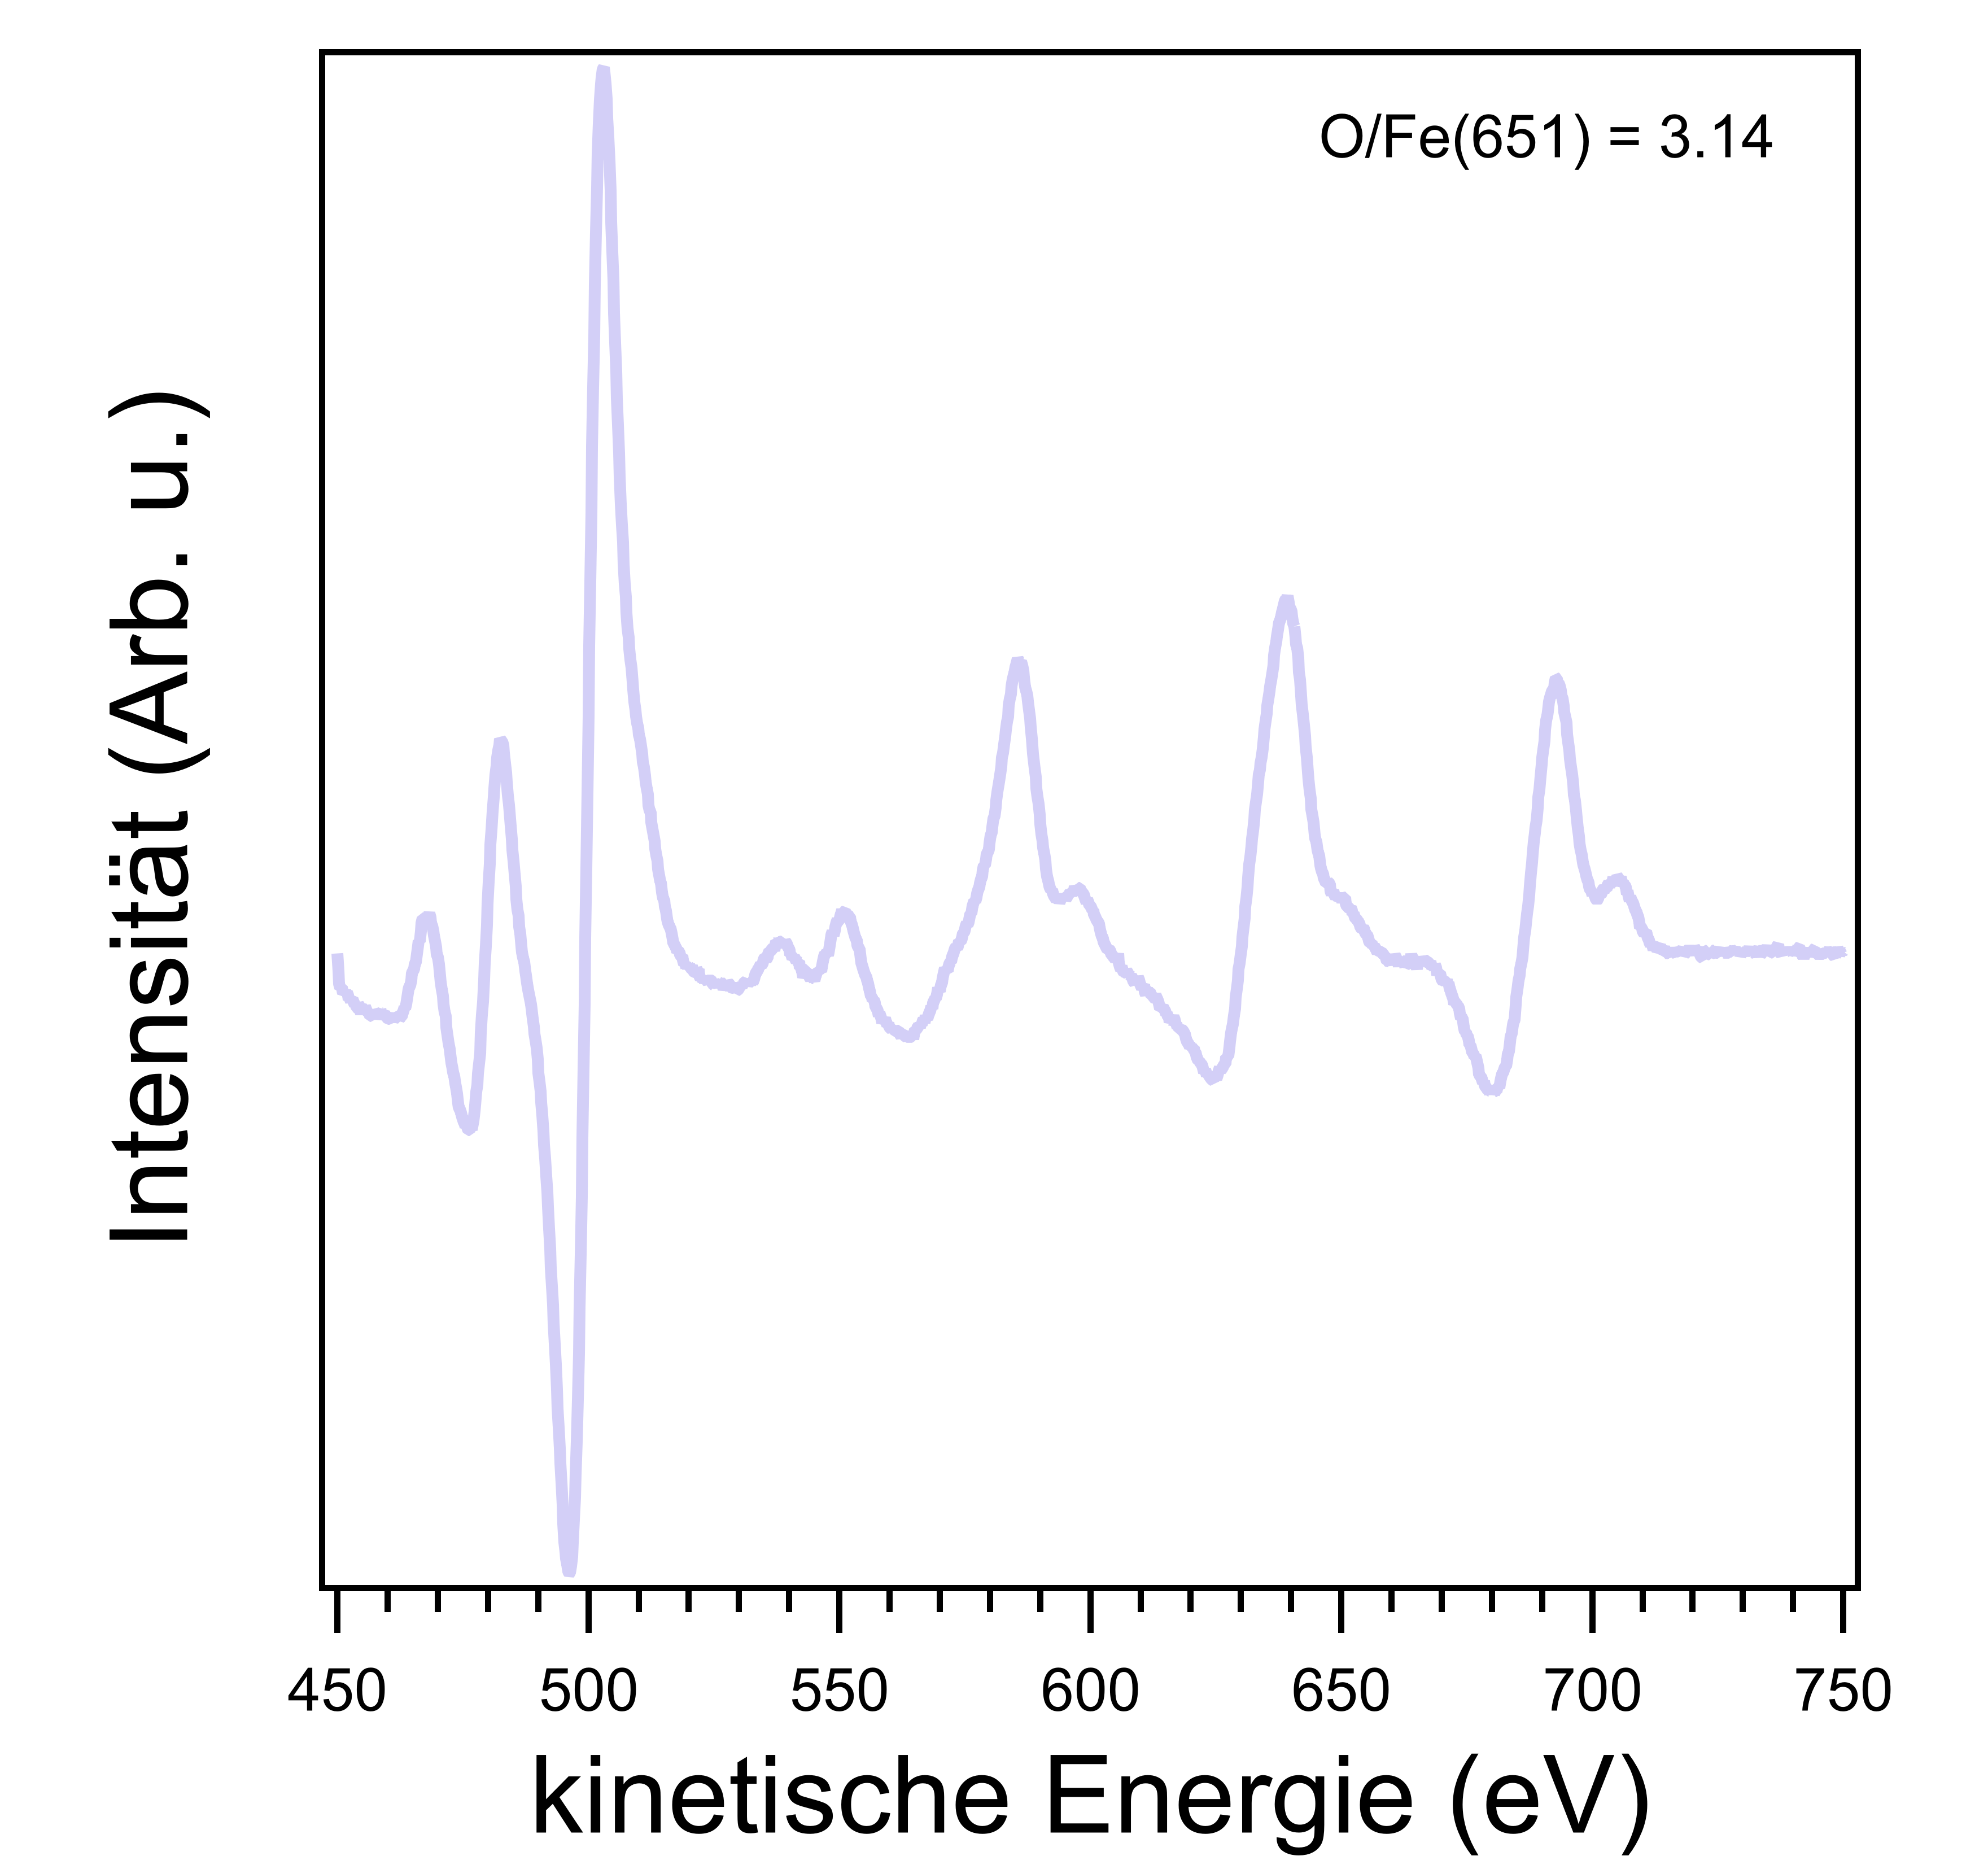
\includegraphics[height=5cm]{./content/pictures/Fe3O4/AES_Fe3O4.png}
            \caption{Das Augerspektrum der Magnetitprobe.}
            \label{fig:Auger_Fe3O4}
        \end{figure}
        Die Konzentrationen an Sauerstoff und Eisen werden mittels Augerelektronenspektroskopie analysiert.
        So ergibt sich das Augerspektrum in \autoref{fig:Auger_Fe3O4}.
        Das Peakverhältnis zwischen dem Sauerstoffsignal bei \SI{503}{\electronvolt} und dem Signal für Eisen bei \SI{651}{\electronvolt} ergibt einen Wert von \num{3.14}~\cite{FeO_1, Auger}.
        Aus der Literatur ist bekannt das für Magnetit ein Wert von \num{3.86} erwartet wird~\cite{FeO_1}.
        Der ermittelte Wert weicht dabei nach unten ab, was durch das zusätzliche Aufheizen auf \SI{600}{\degree} erklärt werden kann.
        Dabei kommt es zur Umstrukturierung der Oberfläche und in Folge dessen auch zur Desorption von Sauerstoff.

        \begin{figure}
            \centering
            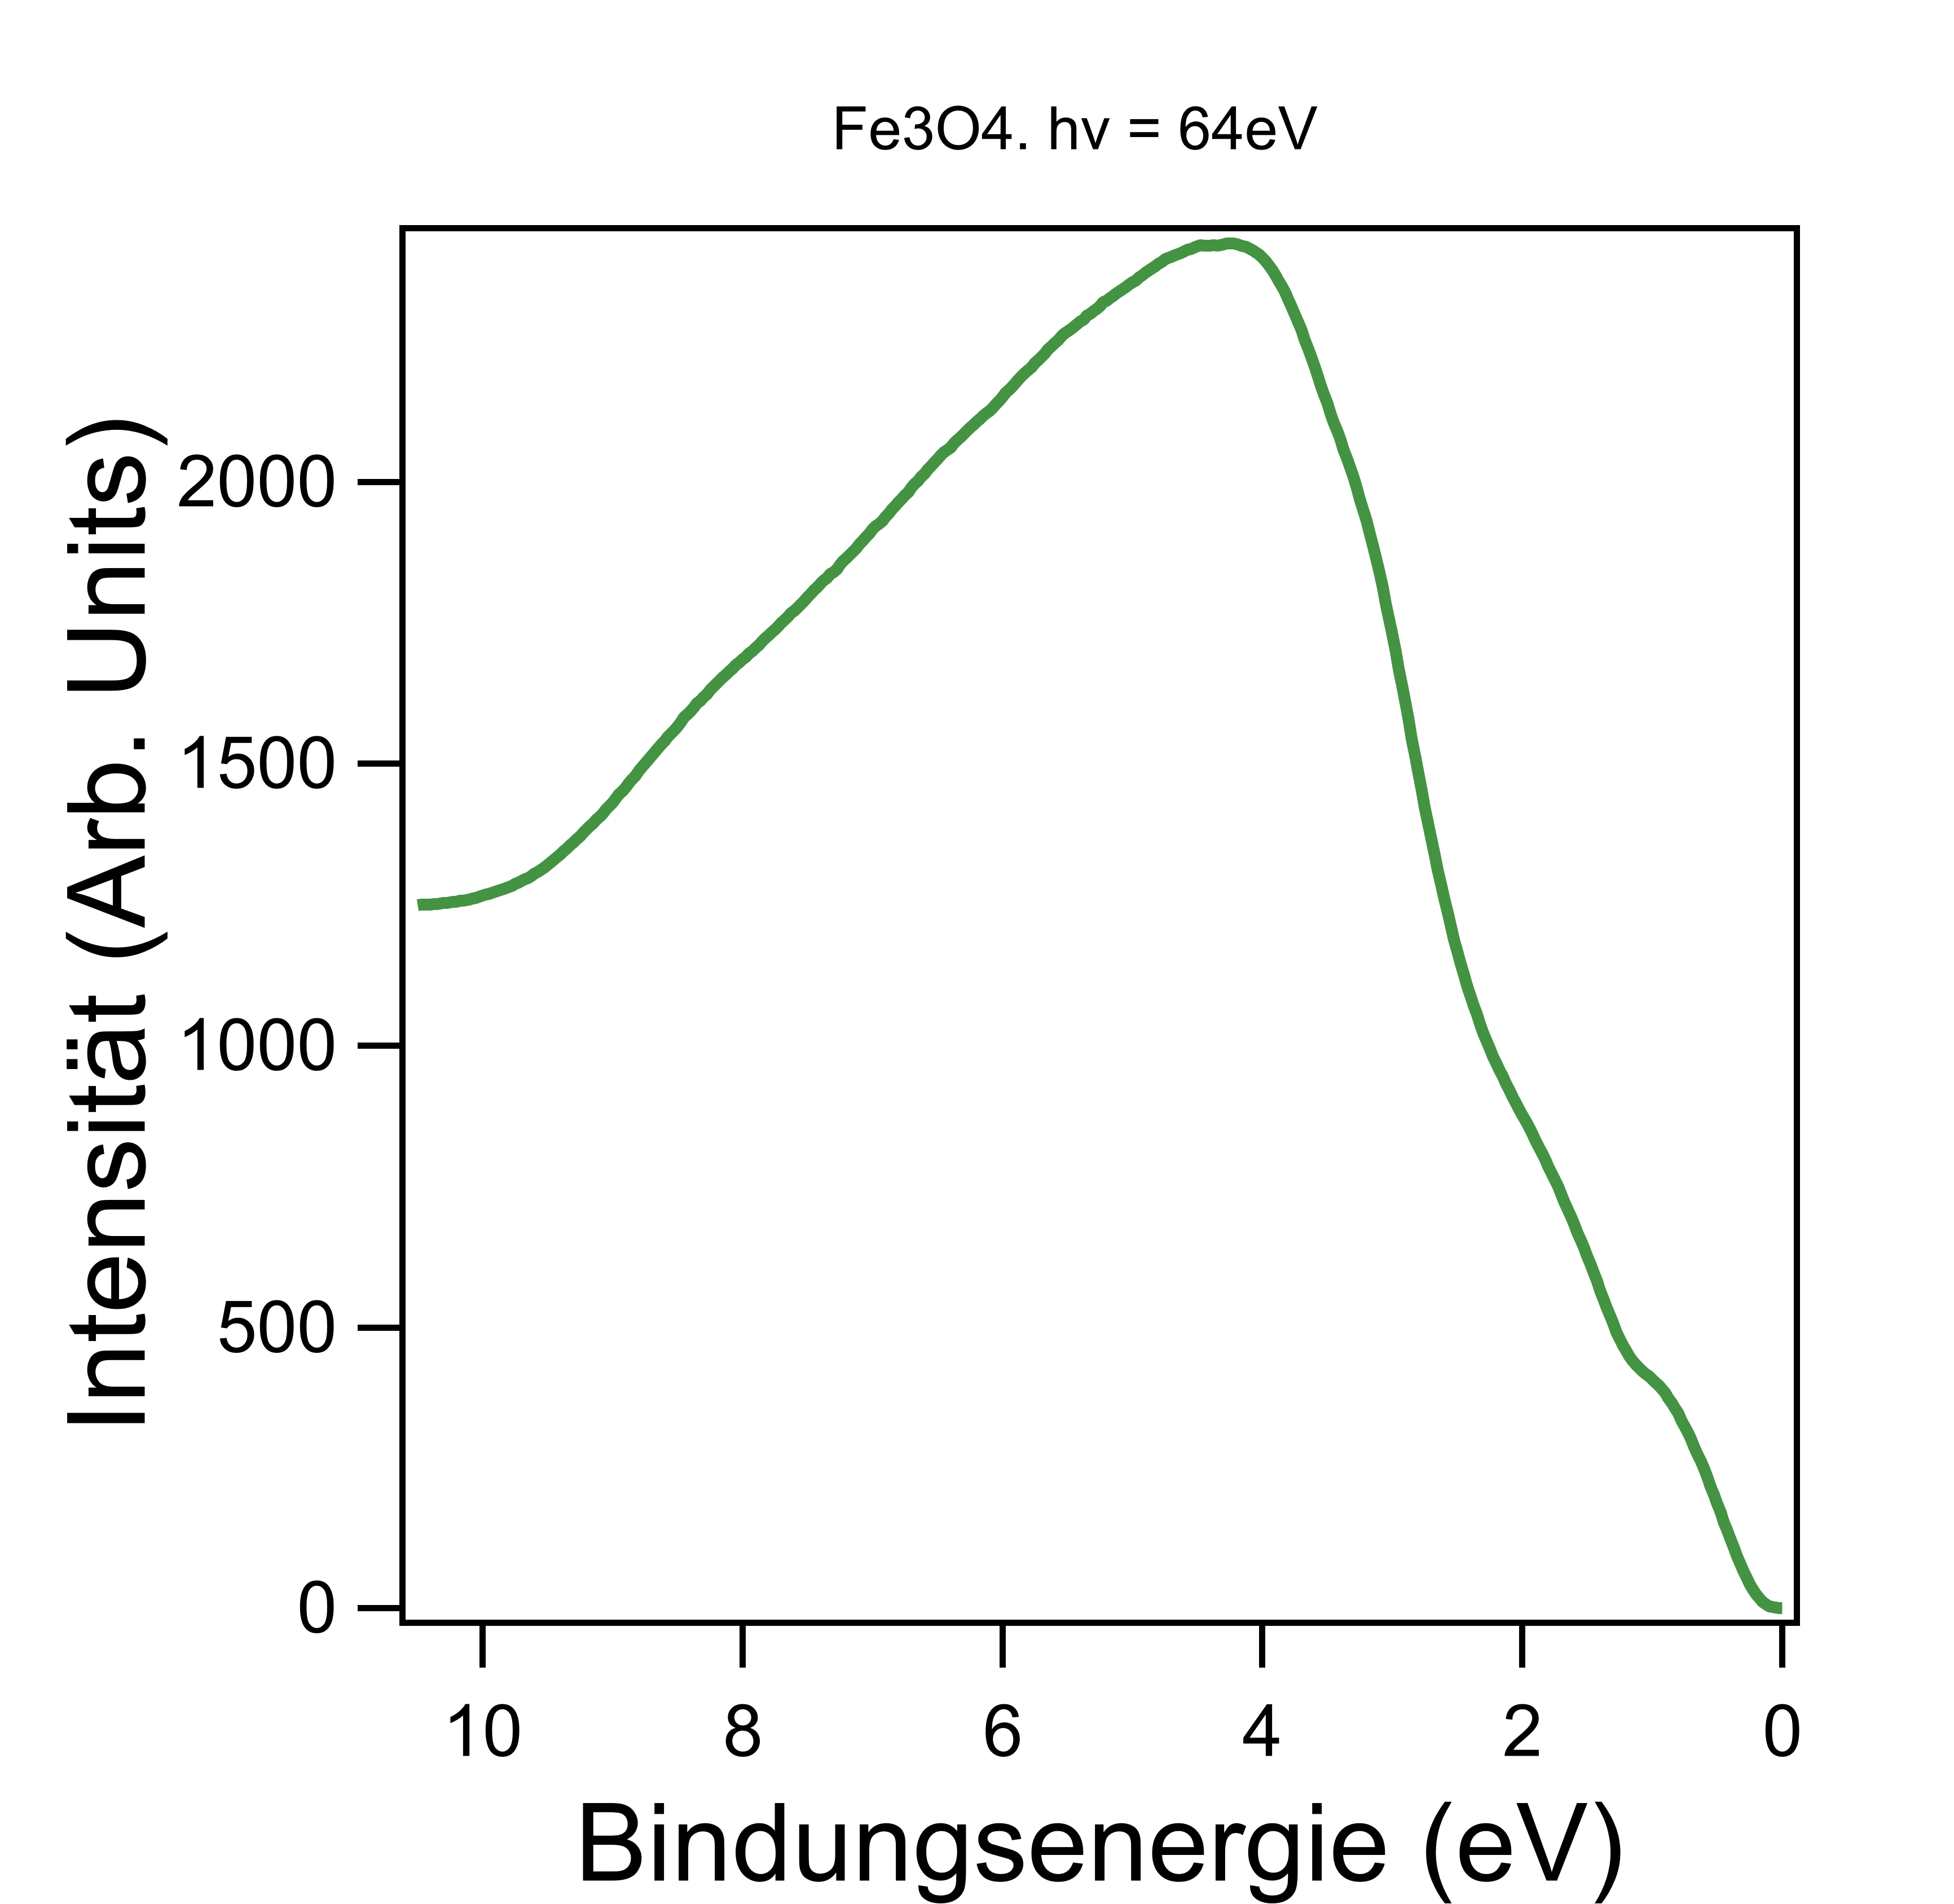
\includegraphics[height=5cm]{./content/pictures/Fe3O4/Fermi_Fe3O4.png}
            \caption{Das Spektrum des valenzbandes bei einer Photonenenergie von \SI{64}{\electronvolt} des \ce{Fe3O4}.}
            \label{fig:EDC_Fe3O4}
        \end{figure}
        Wird sich das Valenzband erneut genauer angeschaut so ergibt sich das winkelintegrierte Spektrum in \autoref{fig:EDC_Fe3O4}.
        Zusammen mit dem Ende der Sekundärelektronen ergibt sich die Austrittsarbeit dabei zu \SI{4.35}{\electronvolt}.

        \begin{figure}
            \centering
            \begin{subfigure}[t]{0.48\textwidth}
                \centering
                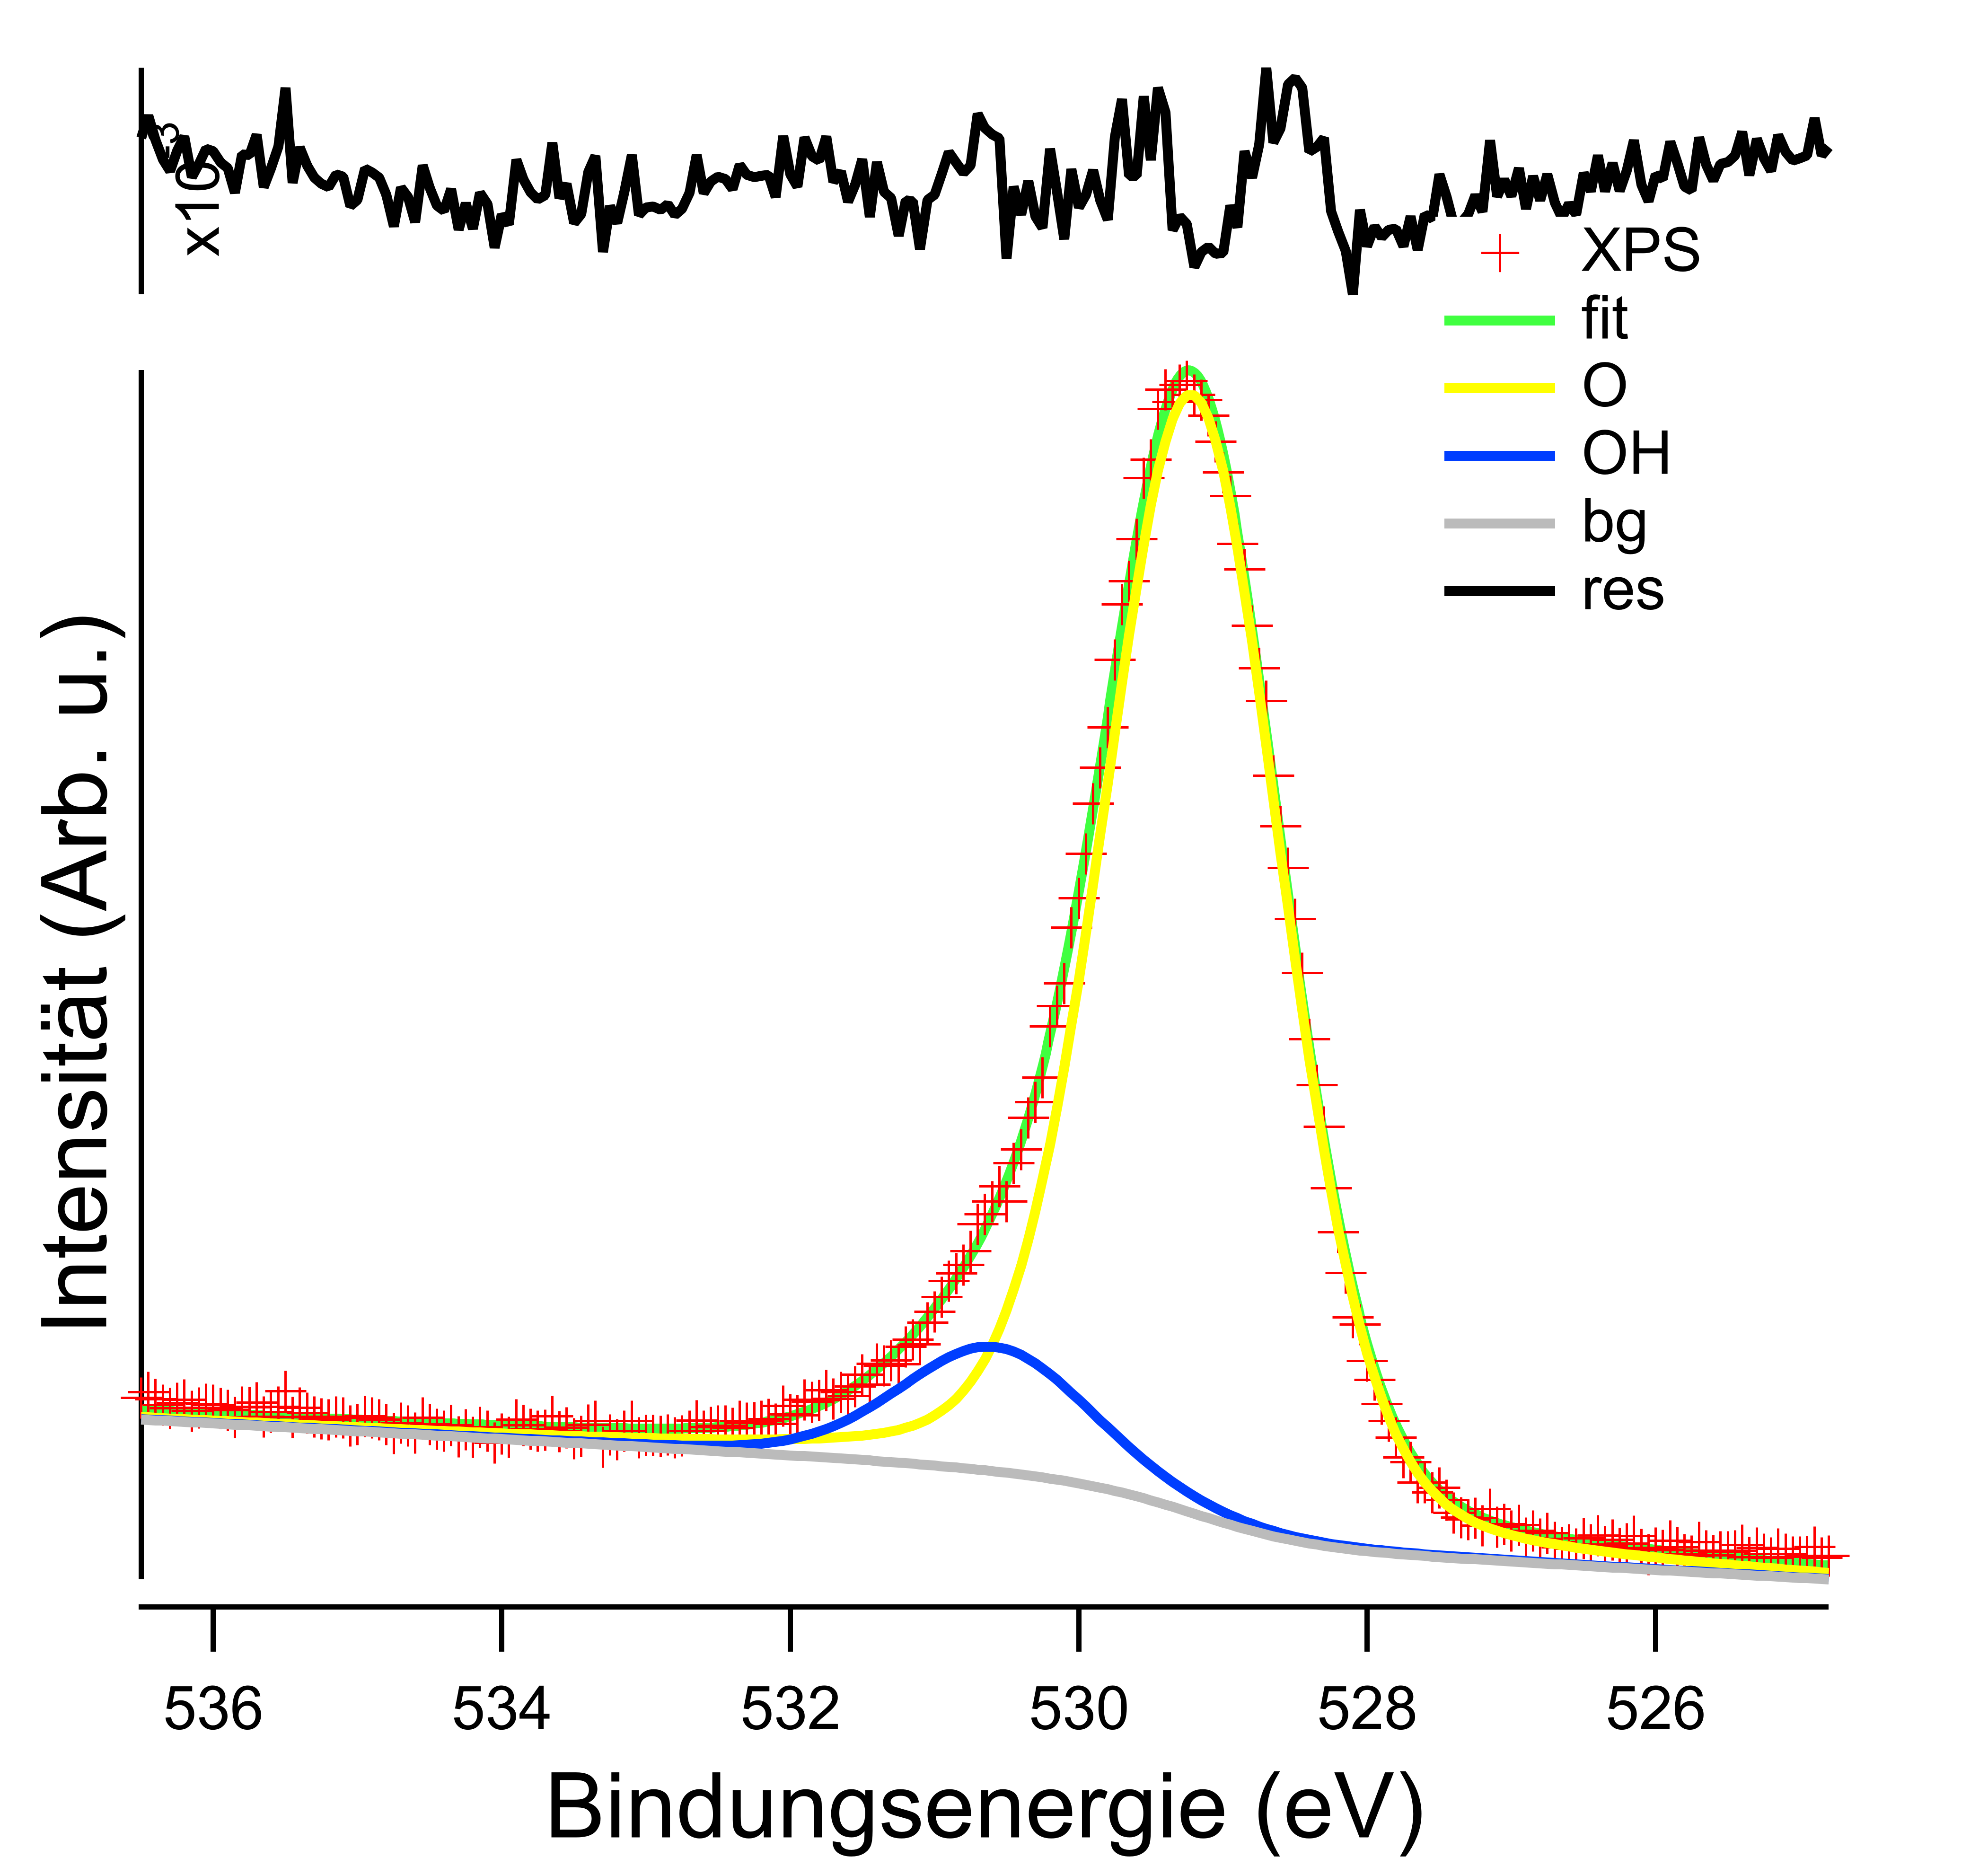
\includegraphics[height=5cm]{./content/pictures/Fe3O4/O1s_Fe3O4.png}
                \subcaption{Spektrum des $\ce{O}_{1\text{s}}$ Übergang. Fit mit zwei Peaks (kleiner Shirley) sehr gut (einer O, der andere OH - Kontamination evtl vom Aufdampfen?).}
                \label{fig:XPSO1s_Fe3O4}
            \end{subfigure}
            \begin{subfigure}[t]{0.48\textwidth}
                \centering
                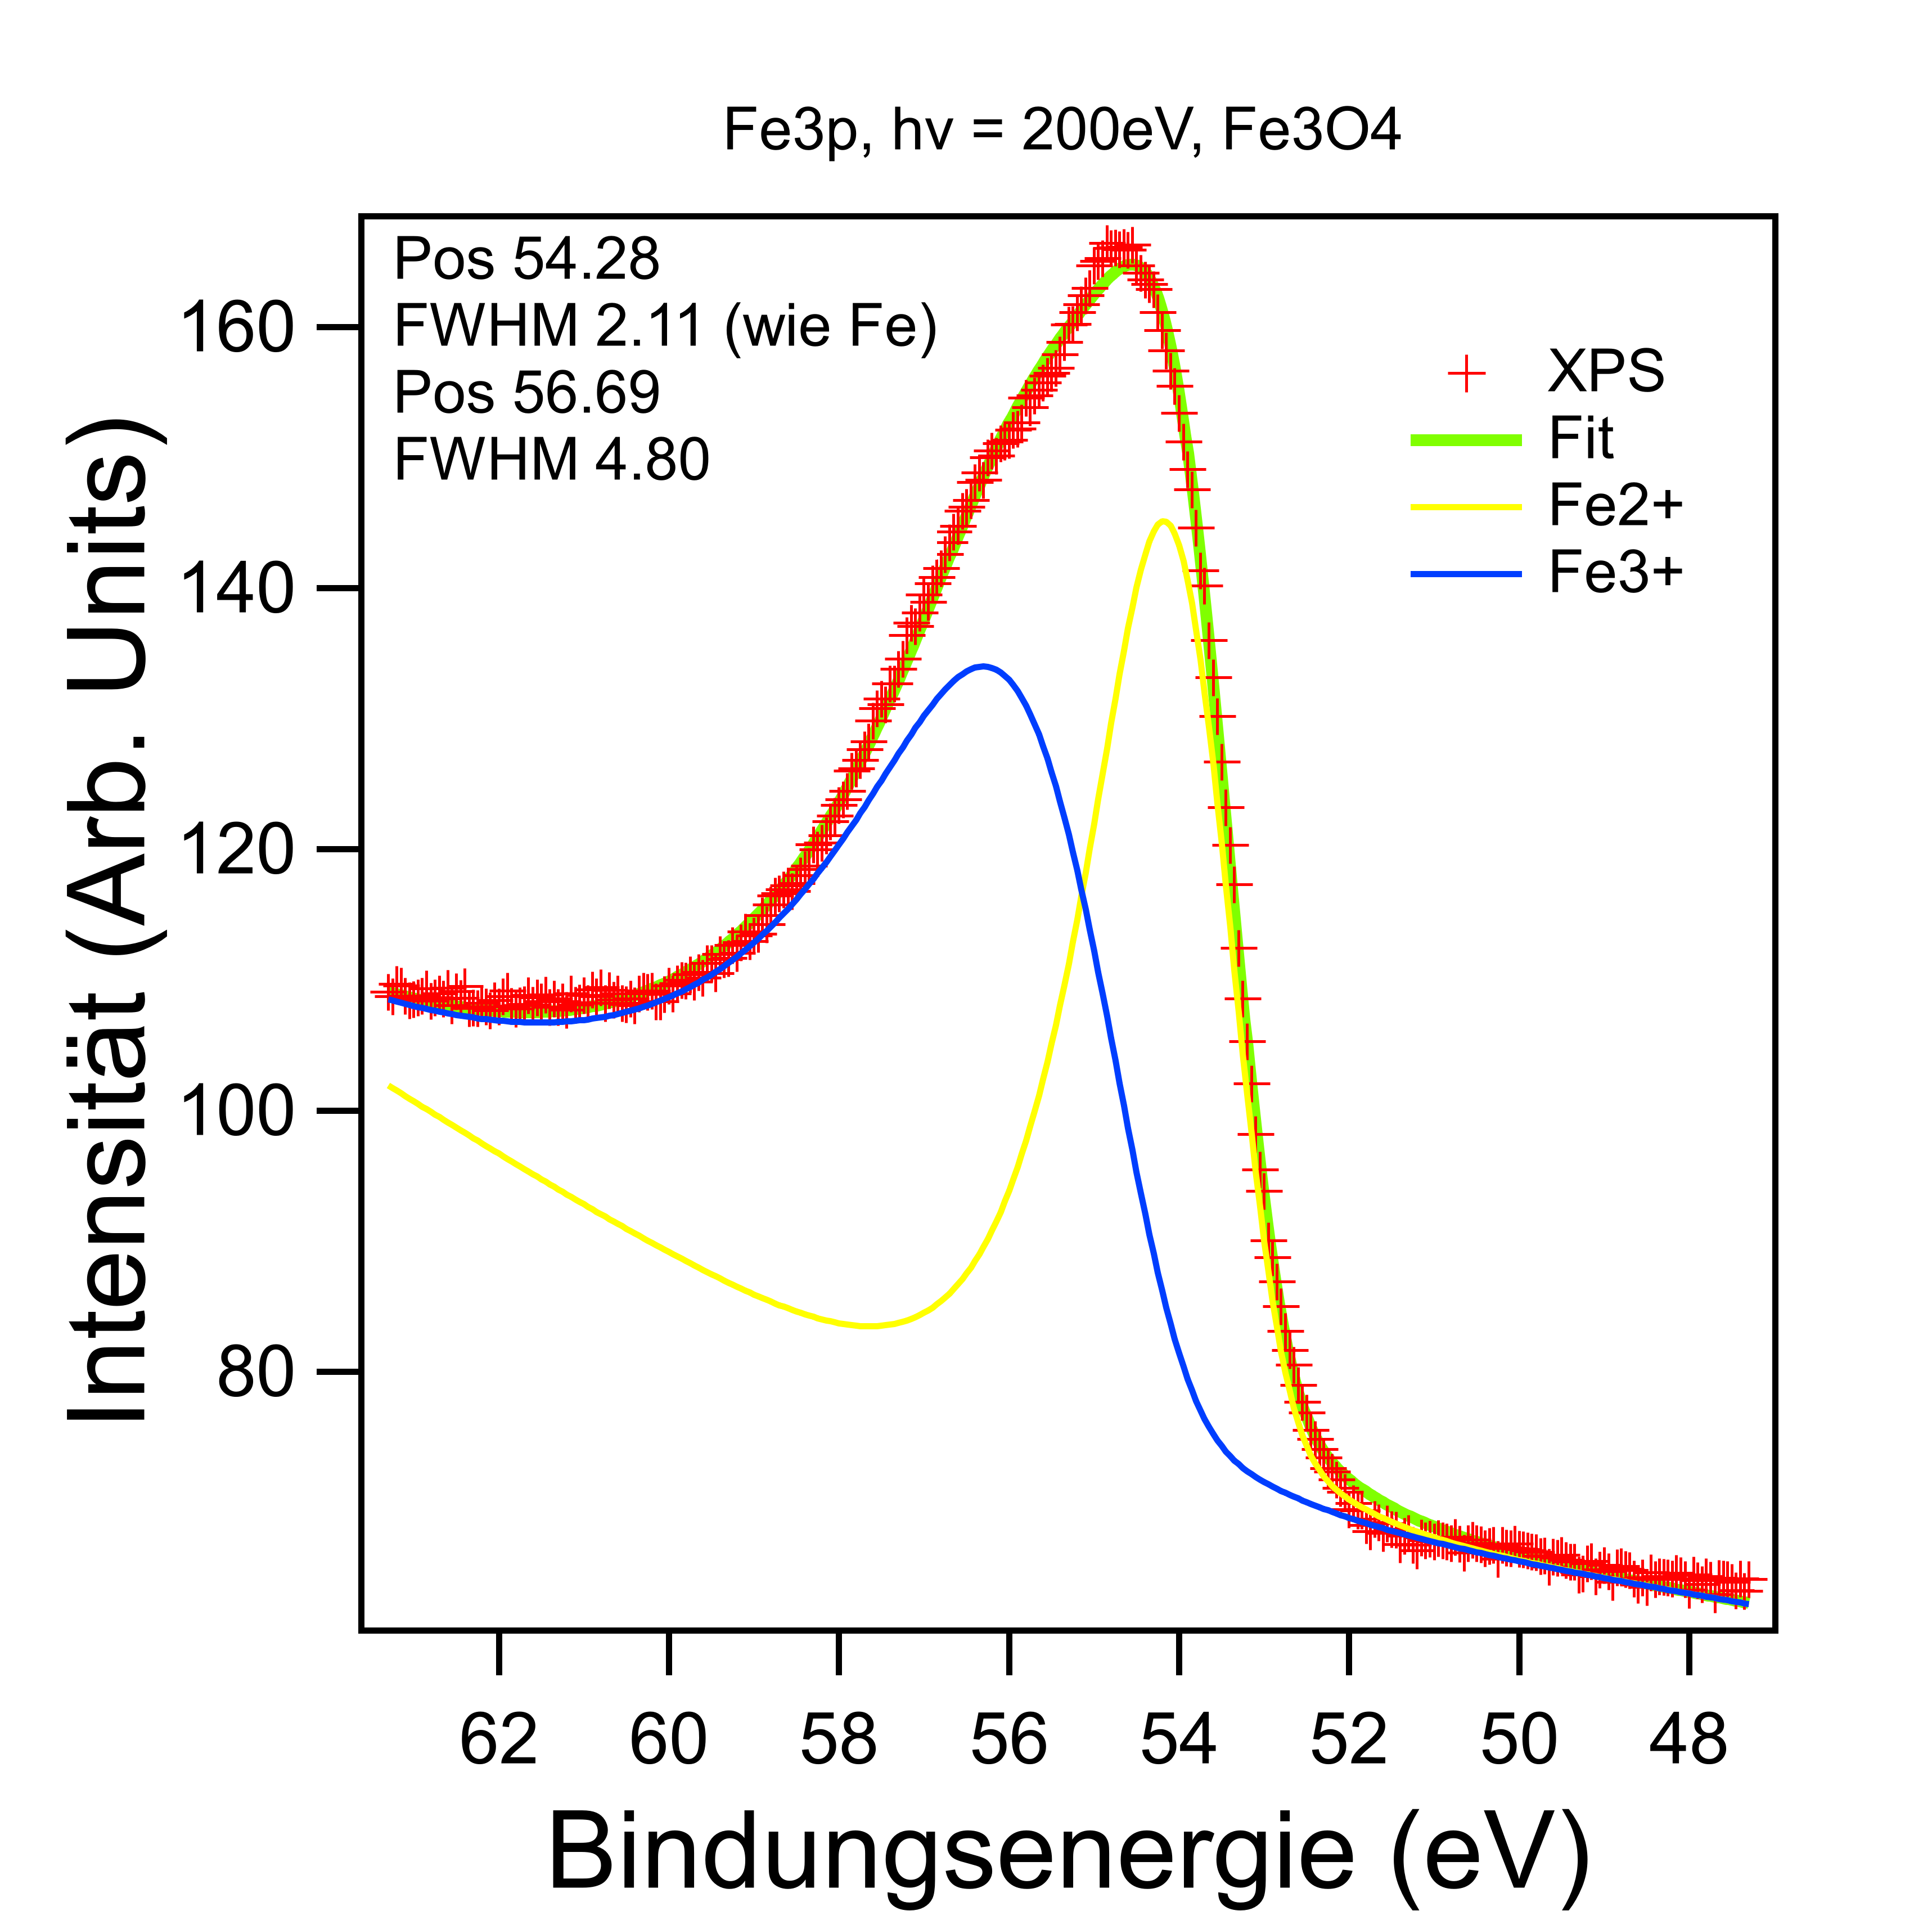
\includegraphics[height=5cm]{./content/pictures/Fe3O4/Fe3p_Fe3O4.png}
                \subcaption{Spektrum des $\ce{Fe}_{3\text{p}}$ Übergang. Gleiches Problem wie beim \ce{FeO} (s. \autoref{fig:XPSFe3p_Fe}) funktioniert abenfalls besser mit Tougaard als Shirley.}
                \label{fig:XPSFe3p_Fe3O4}
            \end{subfigure}
            \caption{Die XPS Spektren der Kernniveaus für das Magnetit.}
            \label{fig:XPS_Fe3O4}
        \end{figure}
        Um genauer zu überprüfen wird auch die chemisch sensetive Methode der Röntgenphotoelektronenspektroskopie angewendet.
        Die entsprechenden Spektren des $\ce{O}_{1\text{s}}$ Signals, sowie des $\ce{Fe}_{3\text{p}}$ Signals sind in \autoref{fig:XPS_Fe3O4} dargstellt.

        Mit Hilfe des magnetischen Röntgen-Zirkular-Dikorismus und magnetischen Röntgen-Linear-Dikorismus lassen sich die magnetischen Eigeschaften des Substrates untersuchen.
        Beide Spektren der Röntgenabsorptionsmessungen sind in \autoref{fig:XAS_Fe3O4} zu sehen.

        Wie bereits schon bei dem Nickeloxid brachte das Aufdampfen von einer Monolage Pentacene keine geordnete Struktur mit sich.


    \section{Wüstit}
        \begin{figure}
            \centering
            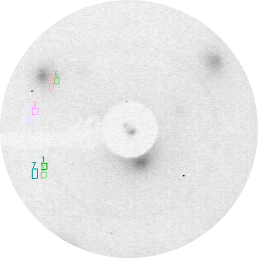
\includegraphics[height=5cm]{./content/pictures/FeO/2021_09_09_004_FeO_44eV.png}
            \caption{\ce{FeO} (100) bei einer Elektronenenergie von \SI{44}{\electronvolt}.}
            \label{fig:LEED_FeO}
        \end{figure}
        Um die Wüstitstruktur zu erhalten wird die Magnetitstruktur zunächst auf \SI{650}{\celsius} aufgeheizt.
        Anschließend werden vermehrt Sauerstoffatome durch ioneninduziertes Zerstäuben ausgelöst um so die Wüstit Zusammensetzung zu erhalten.
        Im anschluss wird die probe nochmal auf \SI{650}{\celsius} erwärmt.
        Dabei entsteht dann das LEED Bild aus \autoref{fig:LEED_FeO}.
        Die Intensitäten sind beim Eisenoxid im Gegensatz zu dem passivierten Eisen invertiert, wobei die zuvor starken Spots nicht mehr sichtbar sind.
        Trotz der gleichen Elektronenenergie von \SI{125}{\electronvolt} sind die Spots leicht nach außen gewandert.
        Dies Widerspricht sich mit der eigentlich größeren Gitterkonstante von Eisenoxid im Bezug auf die $\text{p}(1 \times 1)\ce{O}$ Überstruktur des passivierten Eisens.
        Was dennoch auffällig ist, sind die nicht mehr präsenten zusätzlichen Punkte durch die Überstruktur wie beim \ce{Fe3O4} in \autoref{fig:LEED_Fe3O4}.

        \begin{figure}
            \centering
            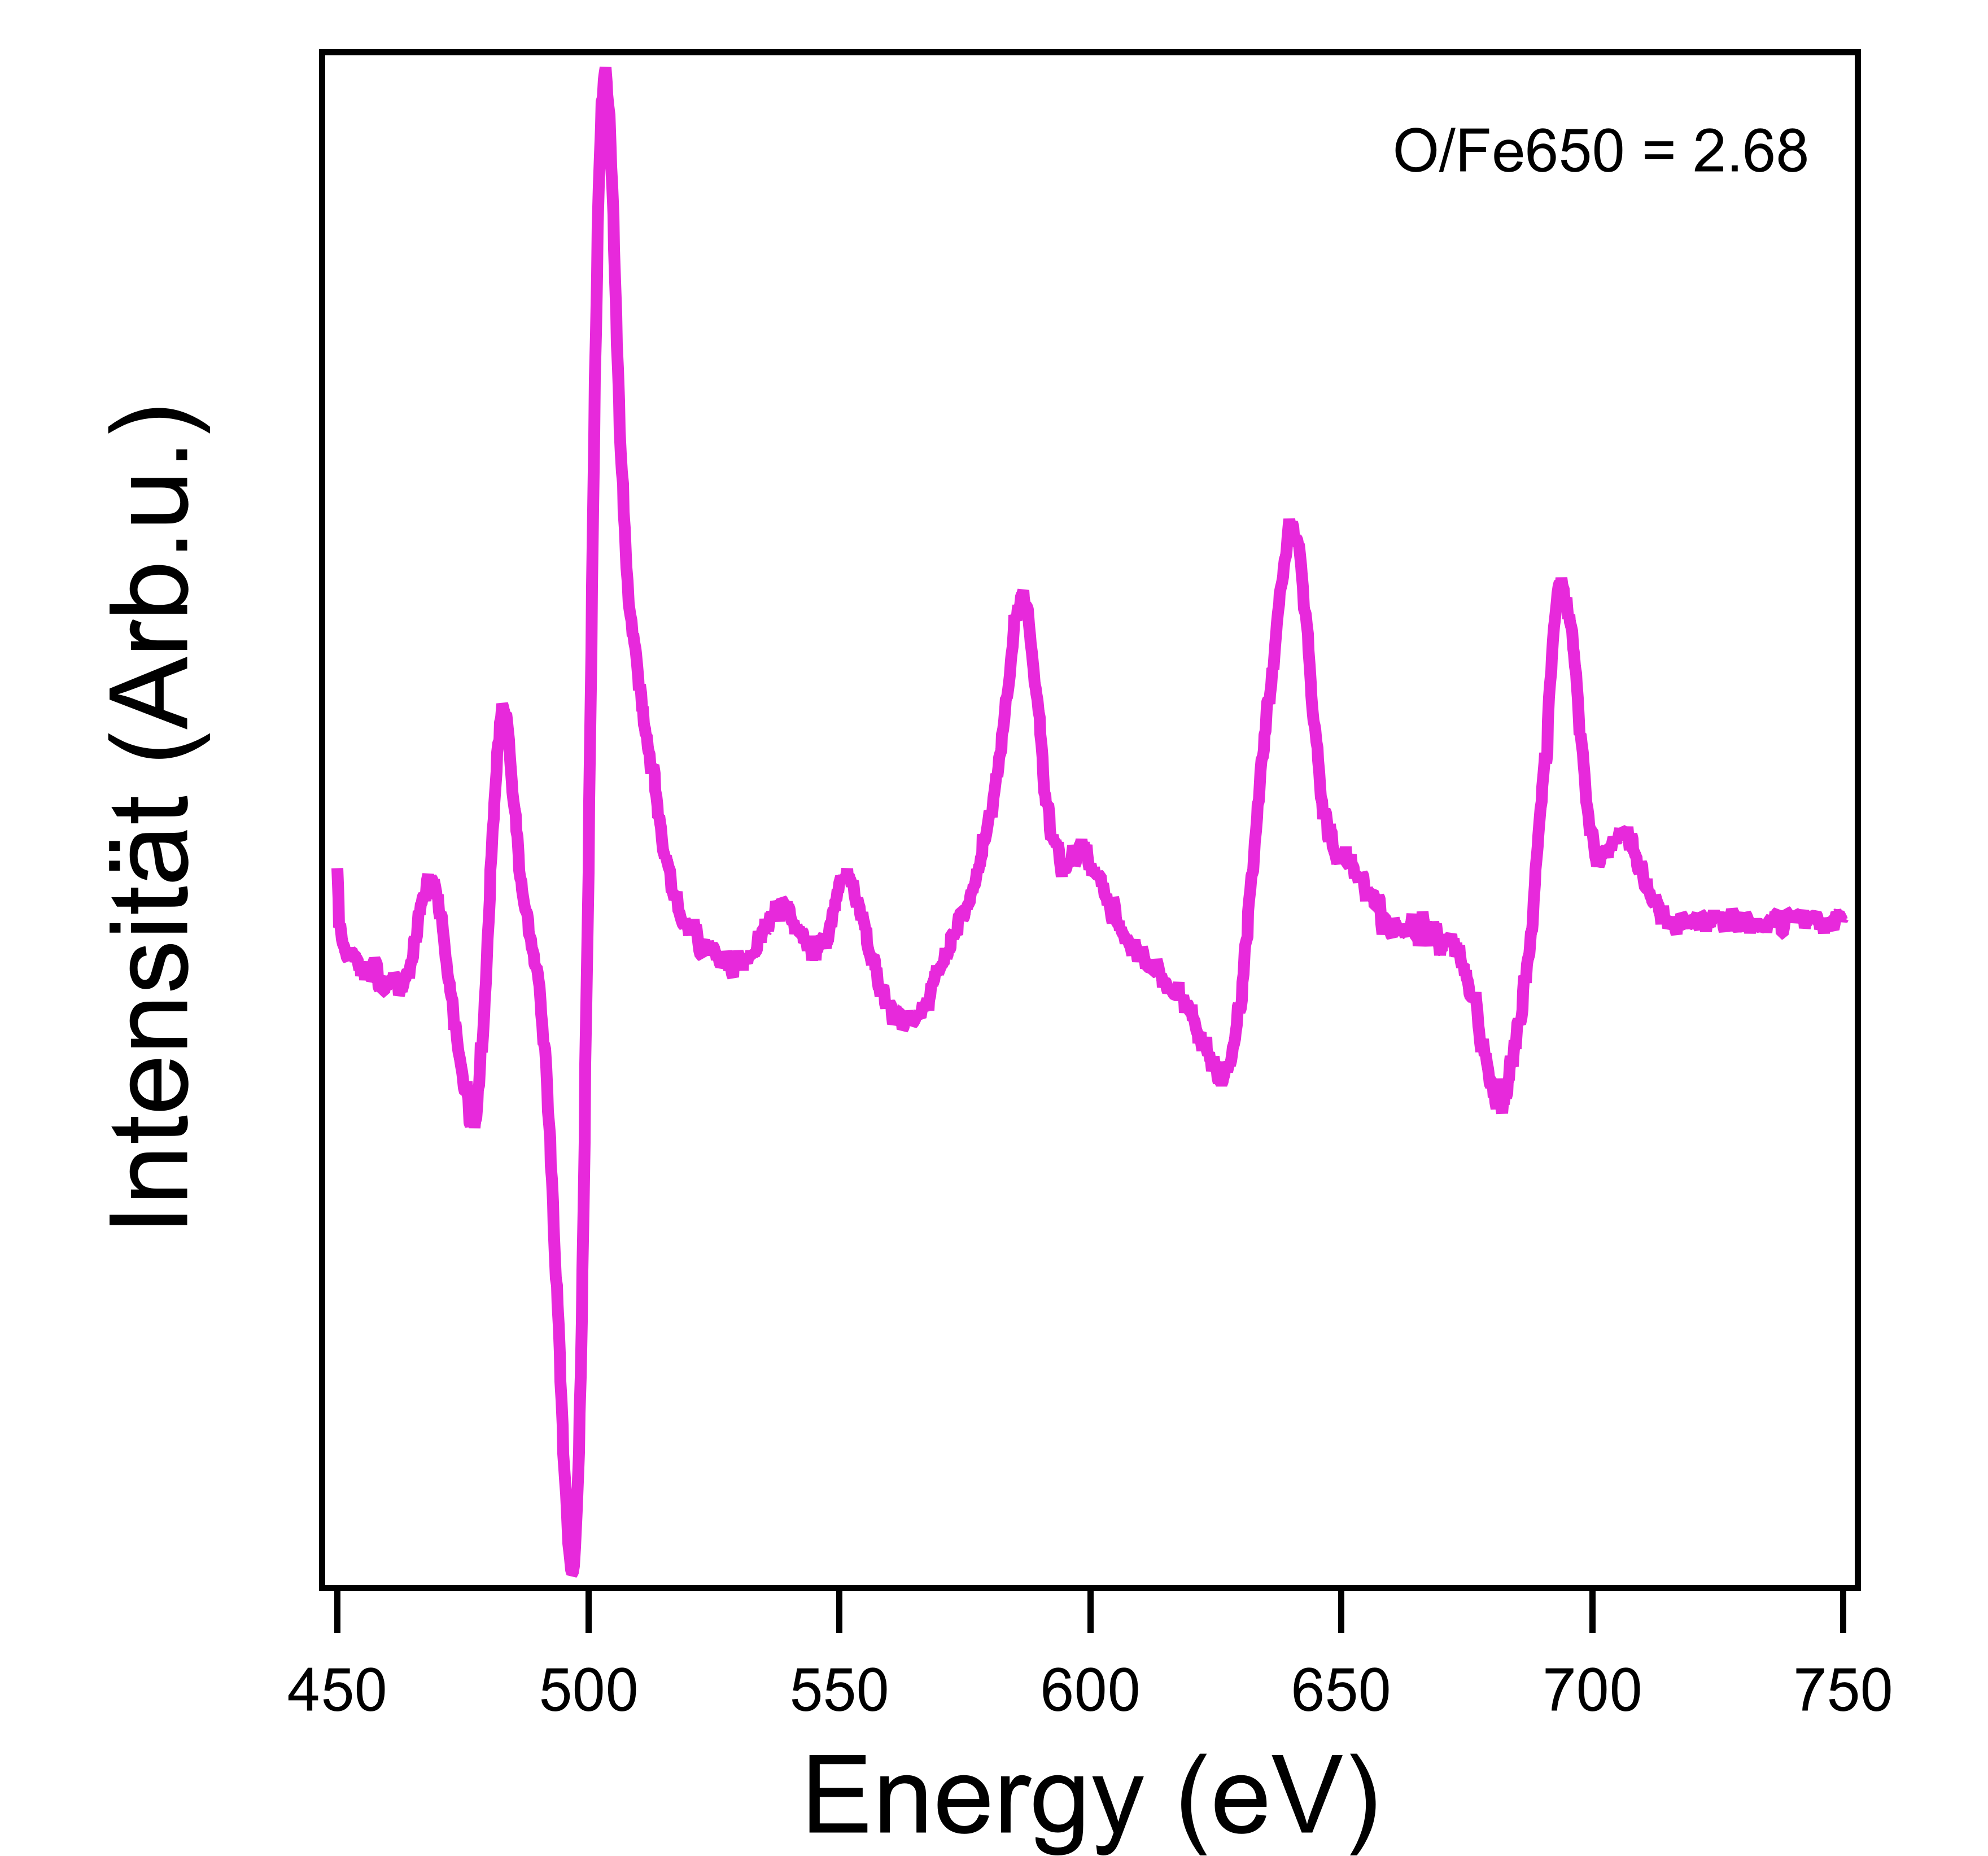
\includegraphics[height=5cm]{./content/pictures/FeO/AES_FeO.png}
            \caption{Das Augerspektrum der Wüstitprobe.}
            \label{fig:Auger_FeO}
        \end{figure}
        \begin{figure}
            \centering
            \begin{subfigure}[t]{0.48\textwidth}
                \centering
                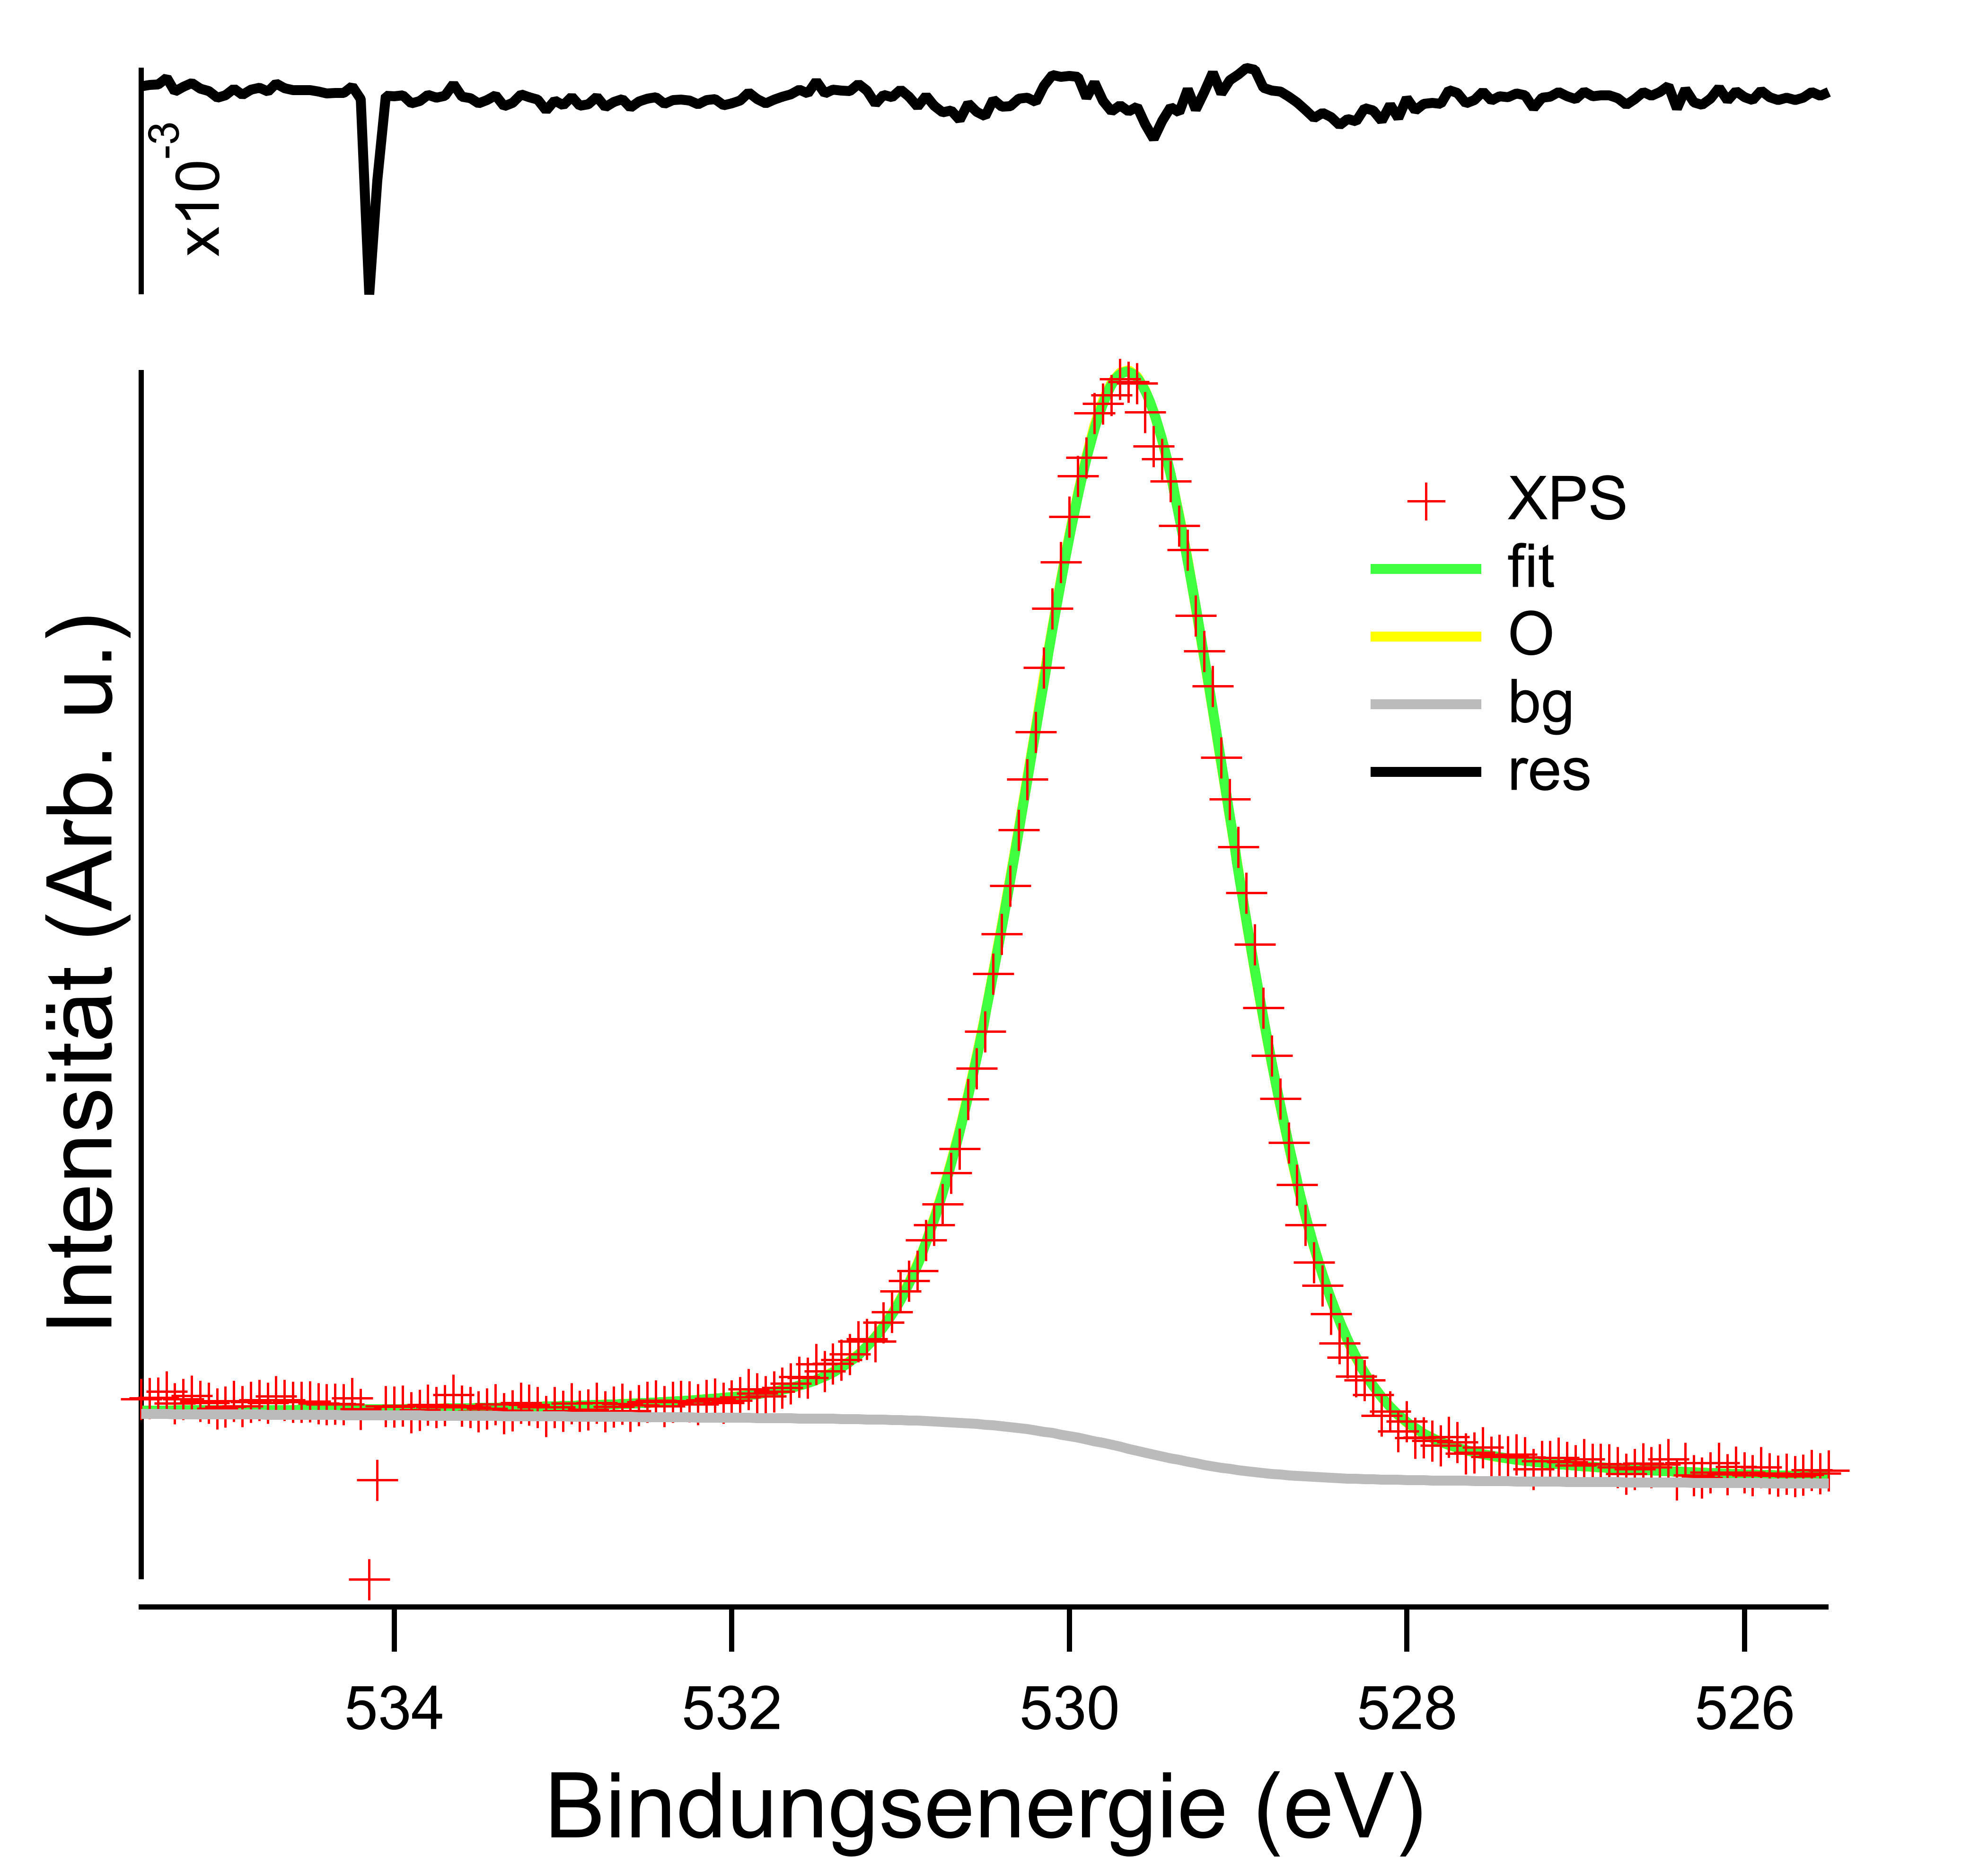
\includegraphics[height=5cm]{./content/pictures/FeO/O1s_FeO.png}
                \subcaption{Spektrum des $\ce{O}_{1\text{s}}$ Übergang. Fit mit einem Peak (kleiner Shirley) sehr gut.}
                \label{fig:XPSO1s_FeO}
            \end{subfigure}
            \begin{subfigure}[t]{0.48\textwidth}
                \centering
                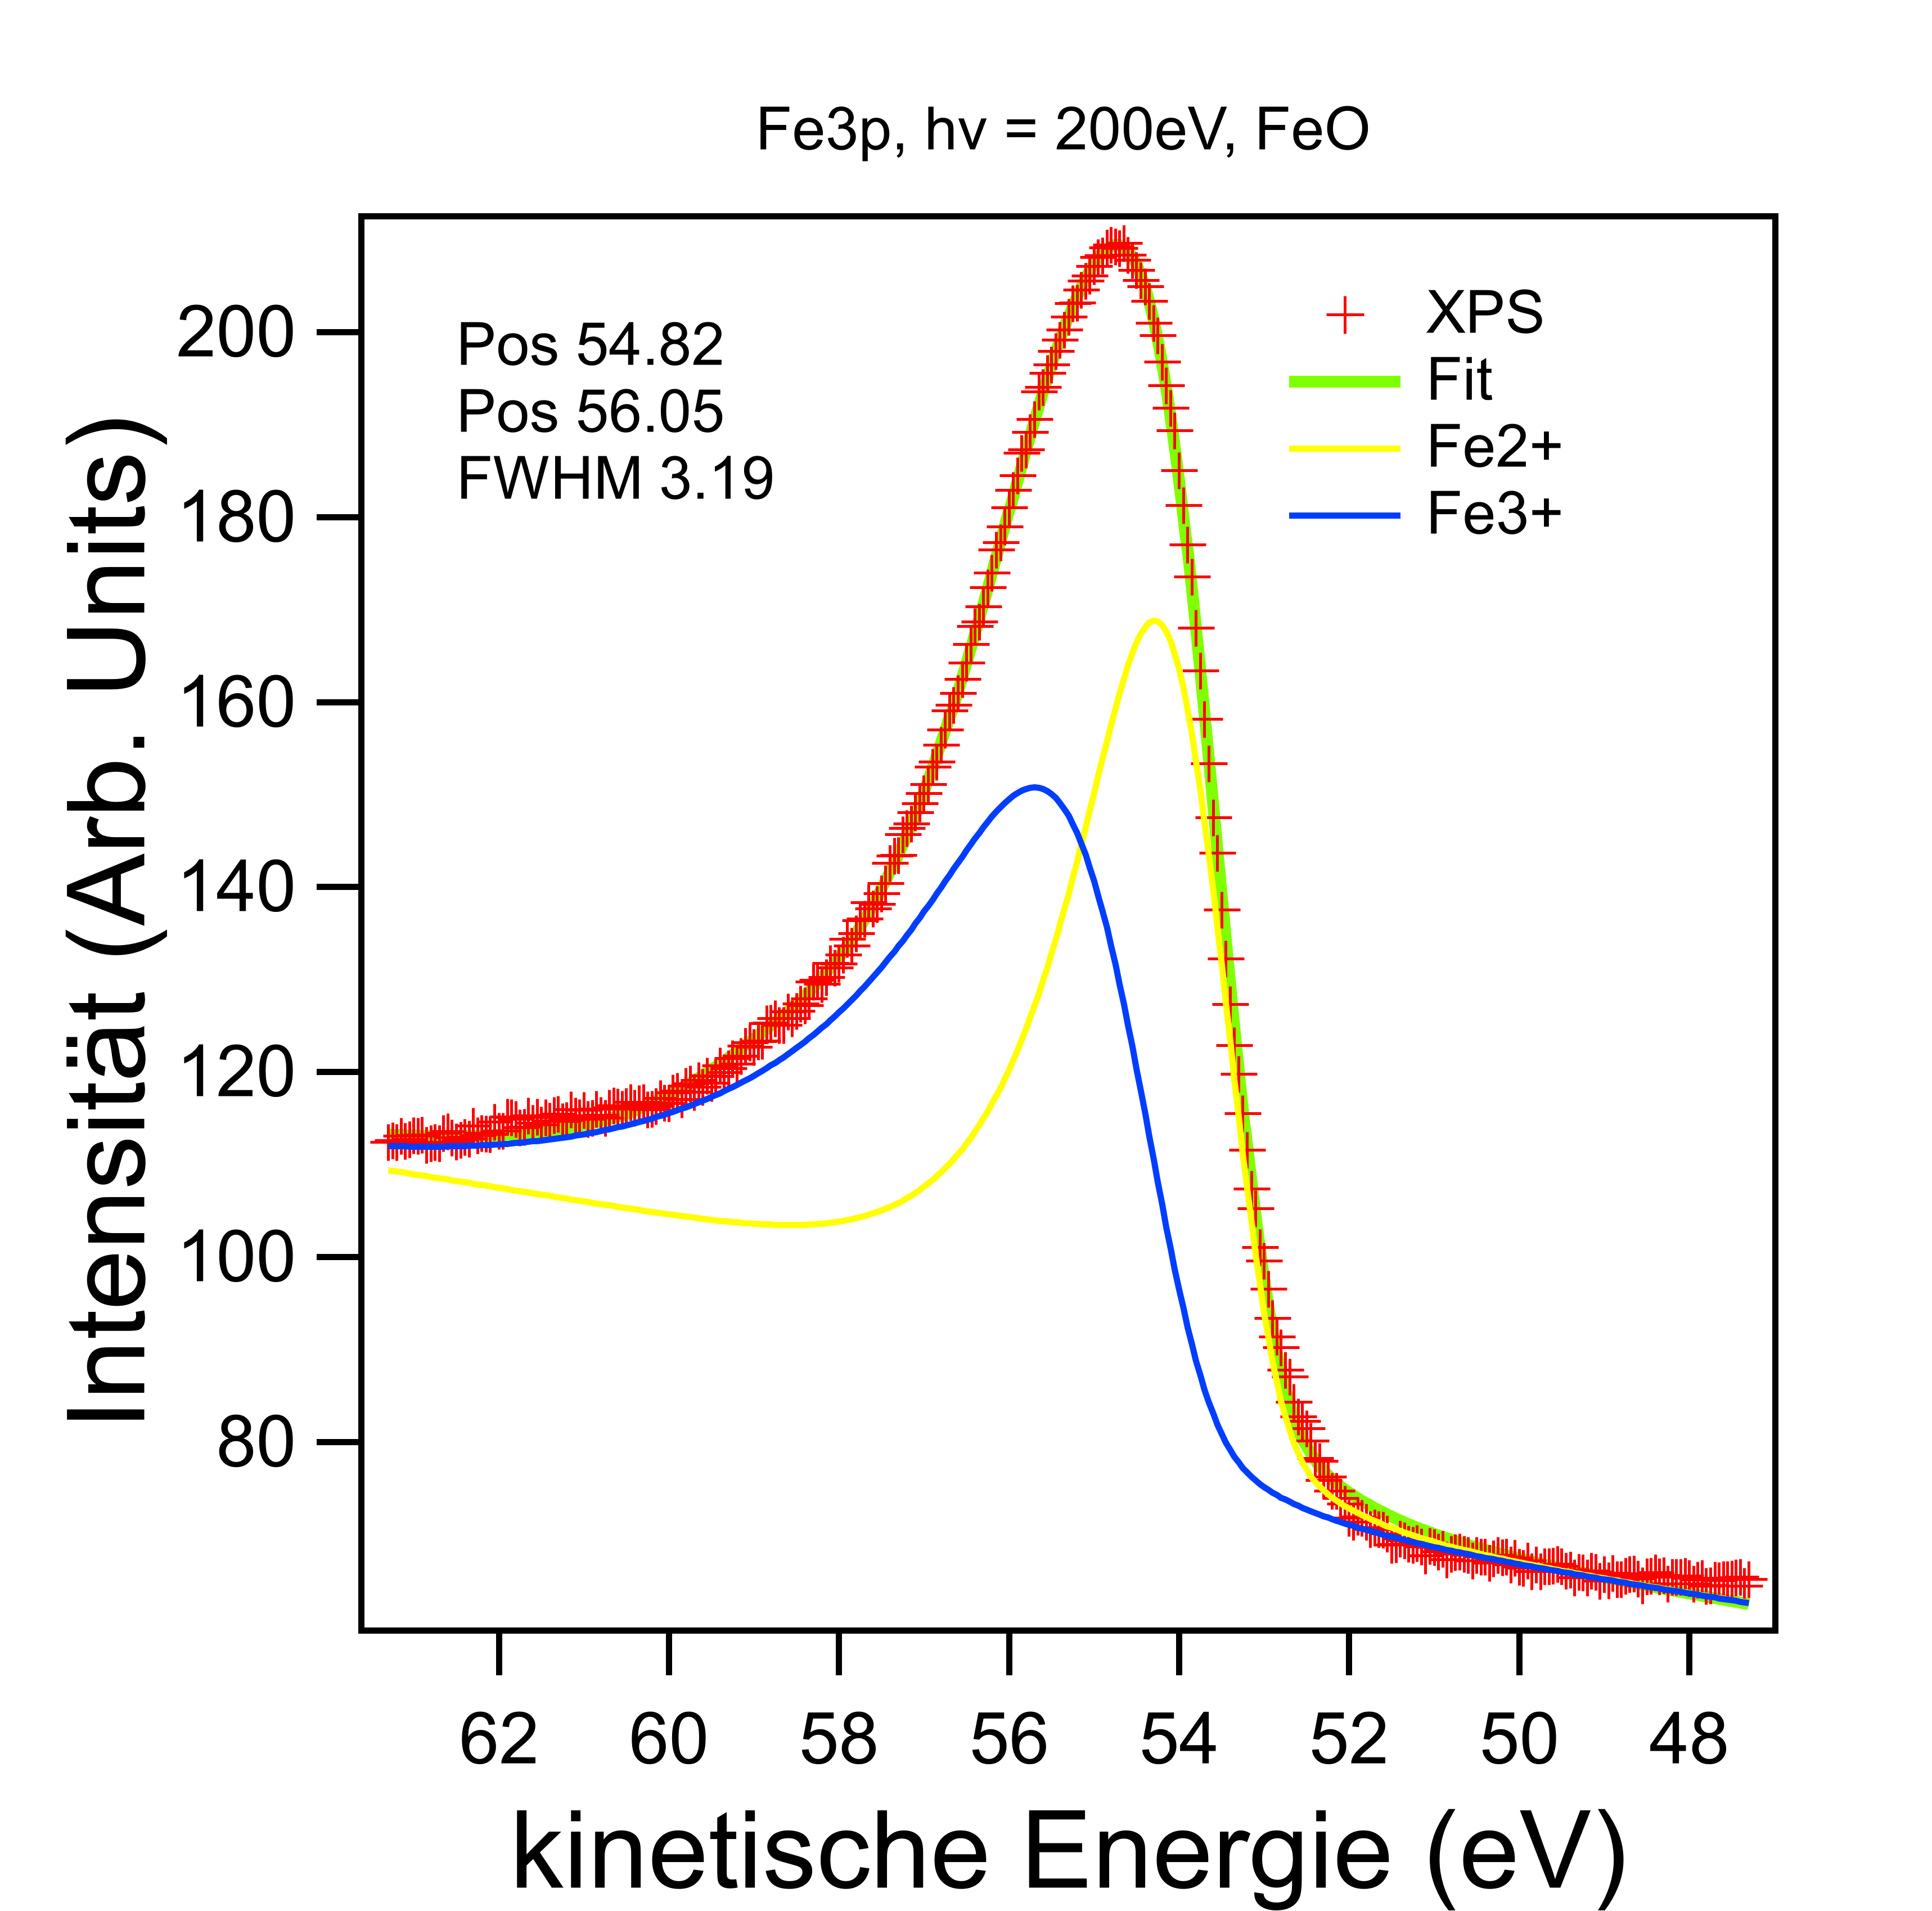
\includegraphics[height=5cm]{./content/pictures/FeO/Fe3p_FeO.png}
                \subcaption{Spektrum des $\ce{Fe}_{3\text{p}}$ Übergang. Zuornung sehr schwierig, ein großer Peak bei kleinen BE und ein kleiner bei großen BE passen. Aber auch zwei etwa gleichgroße Peaks. Je nach dem wie die Parameter gewählt und festgestzt werden.}
                \label{fig:XPSFe3p_FeO}
            \end{subfigure}
            \caption{}
            \label{fig:XPS_FeO}
        \end{figure}
        Das Verhältnis aus Sauerstoff und Eisen kann dabei erneut mittels Augerelektronenspektroskopie überprüft werden.
        Auch das Augerspektrum in \autoref{fig:Auger_FeO} mit dem bereits von Carpa u.A. \cite{FeO_1} entdecken Augerelektronenspektrum für Eisenoxid zeigt gute Übereinstimmung.
        Ebenfalls deutet das Peakverhältnis von dem Sauerstoffsignal und Eisen mit \num{2.53} auf $\ce{FeO}$ hin, da dies nur leicht unterhalb des Wertes aus der Literatur von \num{2.89} liegt \cite{FeO_1}.
        Einen genaueren Einblick welche Struktur vorliegt kann erneut die Röntgenphotoelektronenspektroskopie bieten.
        Die entsprechenden Spektren sind in \autoref{fig:XPS_FeO} zu finden.

        \begin{figure}
            \centering
            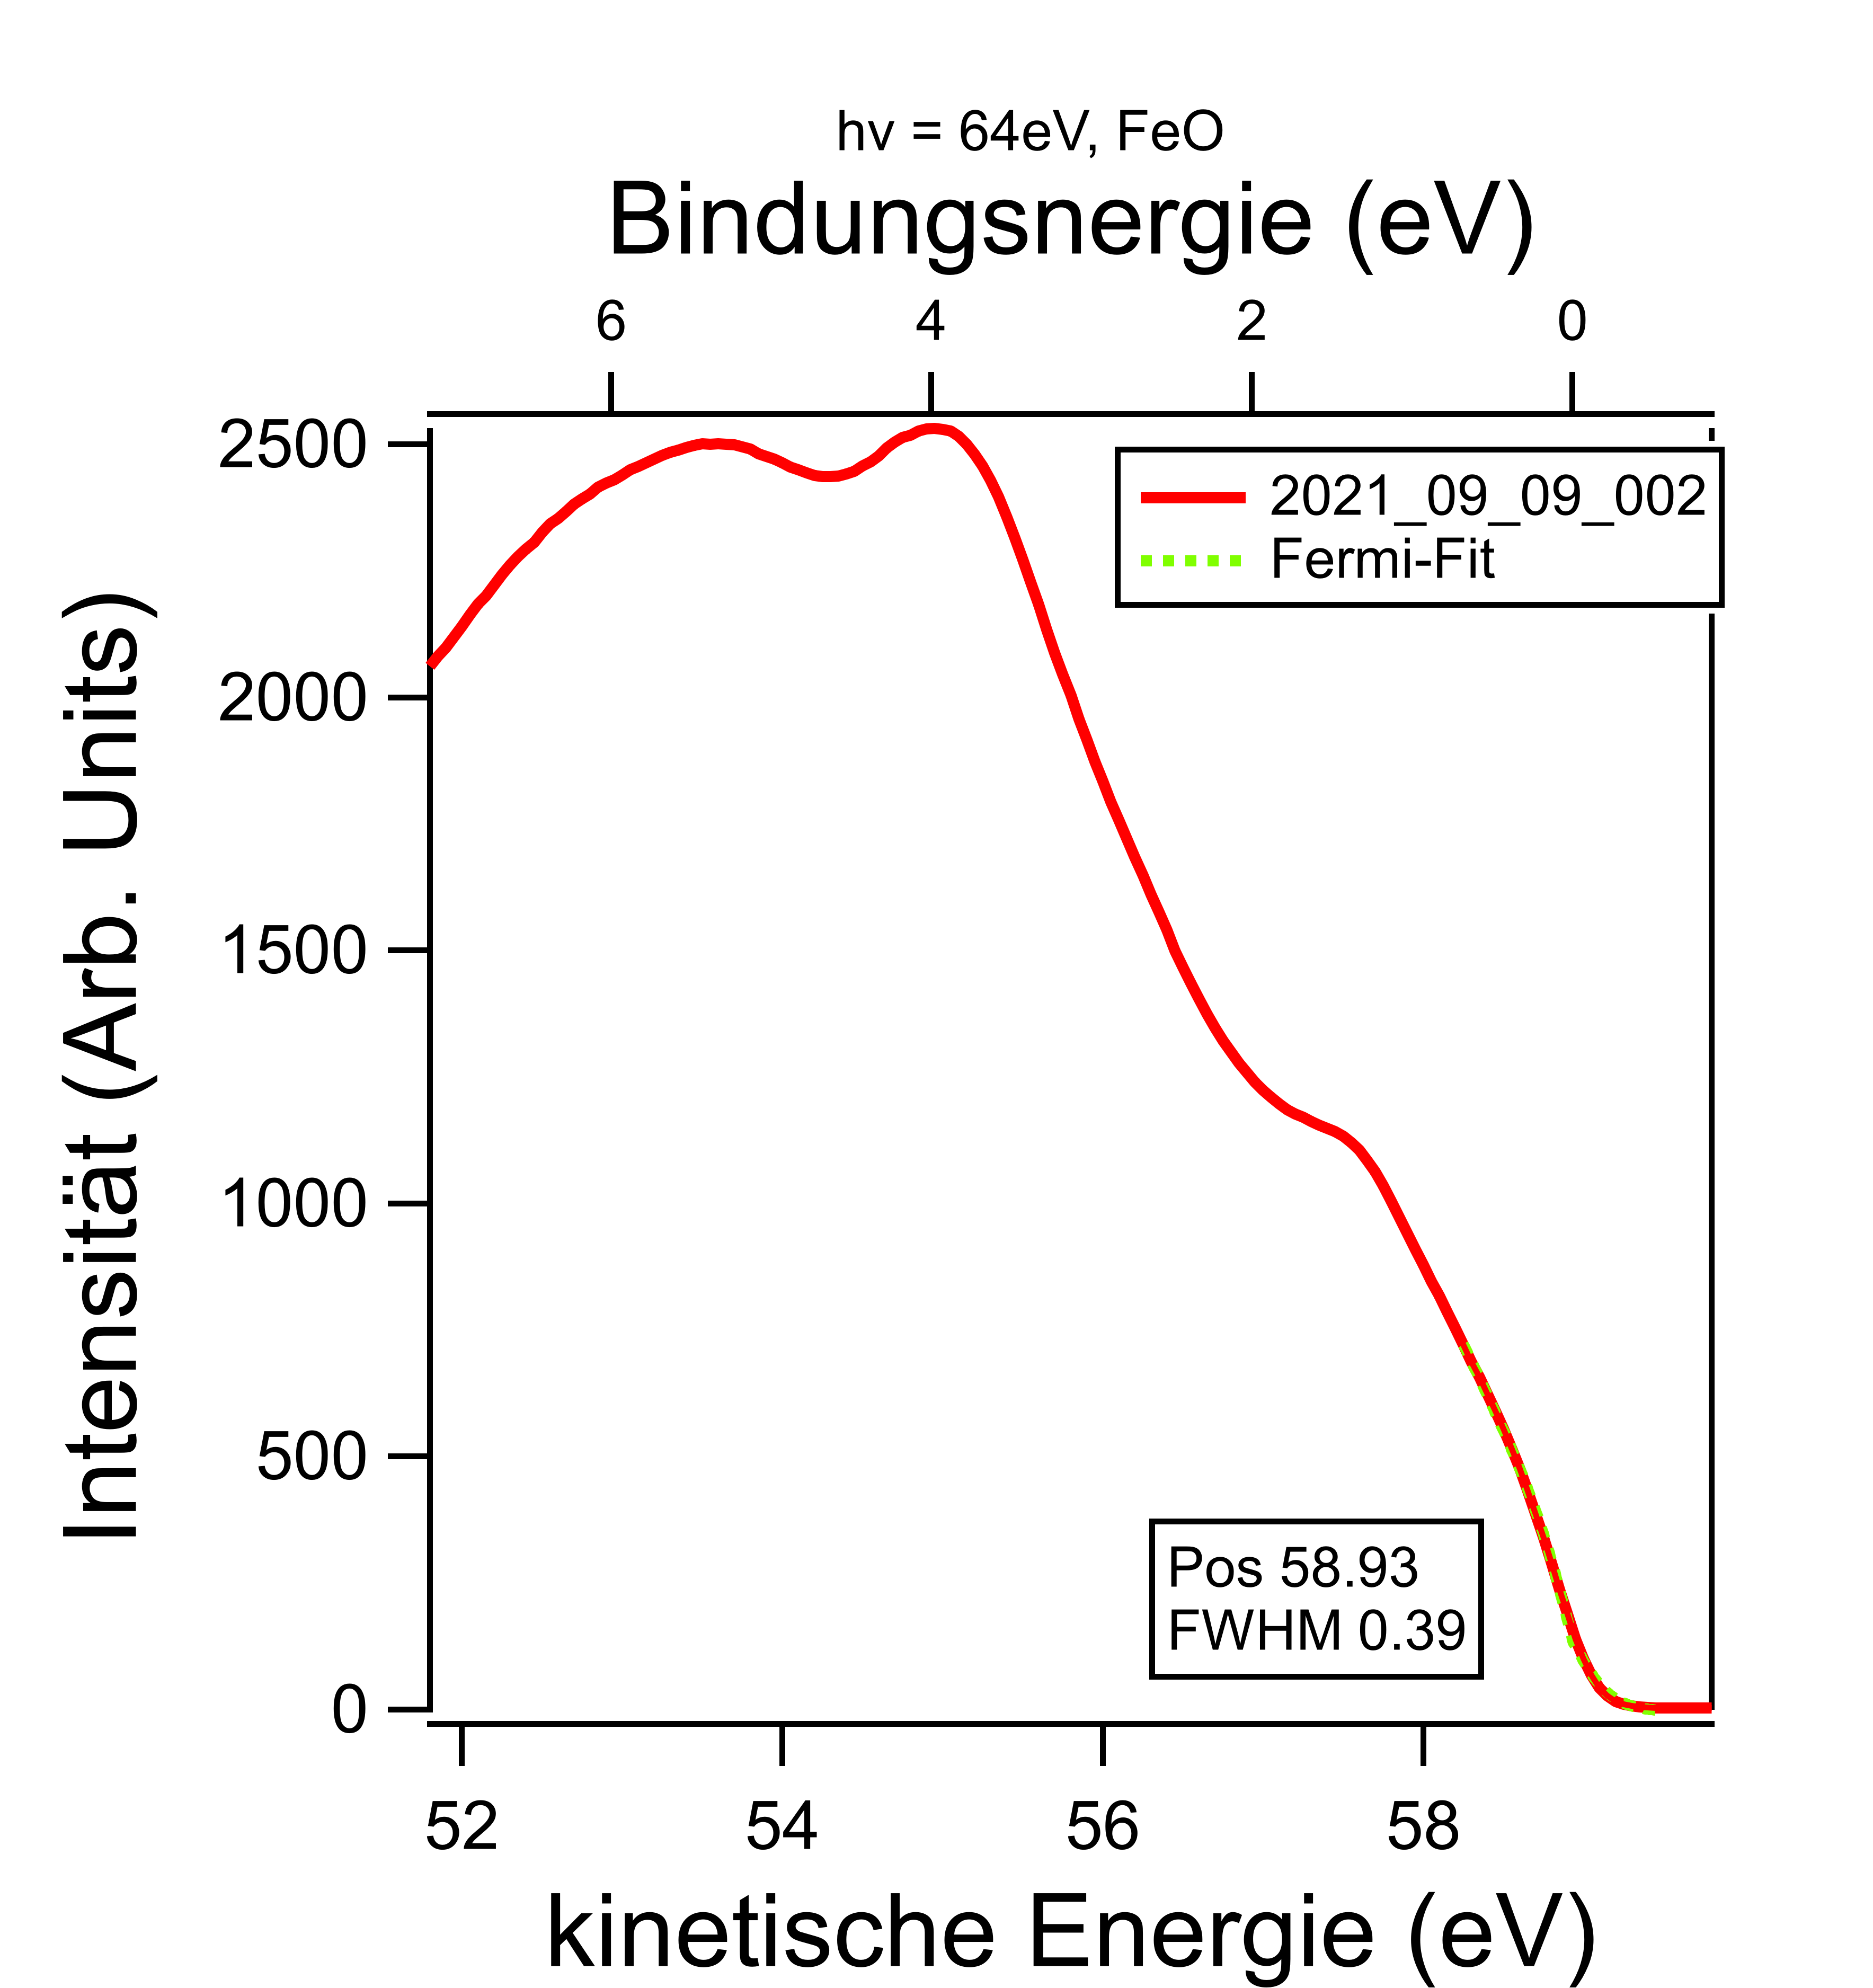
\includegraphics[width=0.5\textwidth]{./content/pictures/FeO/Fermi_FeO.png}
            \caption{Valenzbandspektrum der des \ce{FeO} bei einer Photonenenergie von \SI{64}{\electronvolt}. Zusätzlich eingetragen ist der Fit des Beginns des Spektrums.}
            \label{fig:EDC_FeO}
        \end{figure}
        Ebenso ist in \autoref{fig:EDC_FeO} die Elektronendichtekurve für den Valenzbandbereich des \ce{FeO} aufgetragen.
        Zusätzlich wurde der Beginn des Spektrums in der kinetischen Energie auf \SI{58.93}{\electronvolt} bestimmt.
        Der Beginn des Spektrums sieht einer Fermikante sehr ähnlich.
        Aus dem Punkt an dem die Sekundärelektronen aufhören und der durchs   

        \begin{figure}
            \centering
            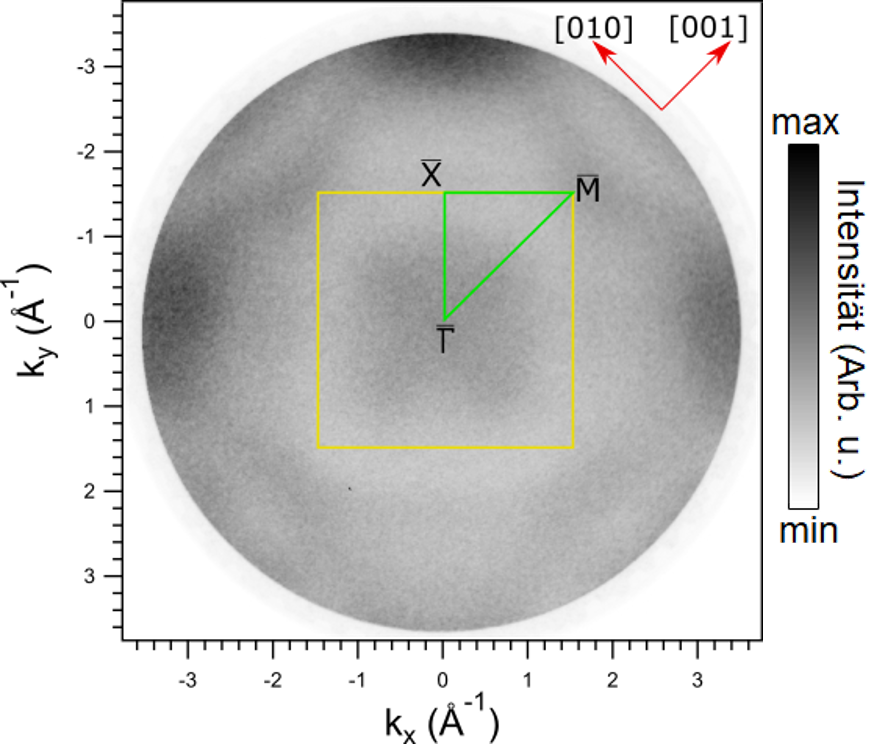
\includegraphics[width=0.5\textwidth]{./content/pictures/FeO/BZ_FeO.png}
            \caption{Die Brillouinzone des Eisensoxid bei einer Bindungsenergie von \SI{1.95}{\electronvolt}.
            Eigezeichnet sind auch die Vektoren, sowie einige Hochsymmetrierichtungen.
            Die Kantenlänge der BZ ist $\frac{2\pi}{a}\sqrt{2} = \SI[per-mode=reciprocal]{2.89}{\per\angstrom}$.
            Im Zentrum liegt der $\overline{\Gamma}$-Punkt, der Abstand zum $\overline{X}$-Punkt ist $\frac{2\pi}{2 \cdot a}\sqrt{2} = \SI[per-mode=reciprocal]{1.45}{\per\angstrom}$ und zum $\overline{M}$-Punkt $\frac{2\pi}{a} = \SI[per-mode=reciprocal]{2.05}{\per\angstrom}$ \cite{Hüfner}.
            \textbf{Problem with px-> k, WKF was Driffting up and down}}
            \label{fig:BZ_FeO}
        \end{figure}
        Auch für das Wüstit lässt sich die Oberflächenbrillouinzone definieren, die in \autoref{fig:BZ_FeO} abgebildet ist.
        ferner auch die Bandstruktur

        \begin{figure}
            \centering
            \includegraphics[height=5cm]{./content/pictures/FeO/XMCD_FeO.png}
            \caption{XAS Spektren für links- und rechtzirkular polarisiertes Licht und ihre Differenz. XMCD}
            \label{fig:XMCD}
        \end{figure}
        \begin{figure}
            \centering
            \includegraphics[height=5cm]{./content/pictures/FeO/XMLD_FeO.png}
            \caption{XAS Spektren für s- und p- polarisiertes Licht, sowie dessen Differenz. XMLD}
            \label{fig:XMLD}
        \end{figure}
        Um sich erneut die magnetischen Eigenschaften des Substrat anzuschauen werden Röntgenabsorptionsmessungen durchgeführt.
        In \autoref{fig:XAS_FeO} sind die entsprechende Spektren dargestellt.
        
        \begin{figure}
            \centering
            \begin{subfigure}[t]{0.48\textwidth}
                \centering
                \includegraphics[height=5cm]{./content/pictures/FeO+5A/FeO_5A_34_80eV.png}
                \subcaption{Das Bild für eine kinetische Energie von \SI{34.80}{\electronvolt}, also \SI{0.70}{\electronvolt} Bindungsenergie.}
            \end{subfigure}
            \begin{subfigure}[t]{0.48\textwidth}
                \centering
                \includegraphics[height=5cm]{./content/pictures/FeO+5A/MO_LUMO_RT_RT.png}
                \subcaption{Das LUMO mit Symmetrisierung zweier um \SI{90}{\degree} verdrehten Übergitter.}
            \end{subfigure}
            \caption{Vergleich der gemessenen Intensitätsverteilung mit der des symmetrisierten LUMO.}
            \label{fig:FeO5A1}
        \end{figure}
        \begin{figure}
            \centering
            \begin{subfigure}[t]{0.48\textwidth}
                \centering
                \includegraphics[height=5cm]{./content/pictures/FeO+5A/FeO_5A_33_75eV.png}
                \subcaption{Das Bild für eine kinetische Energie von \SI{33.75}{\electronvolt}, also \SI{1.75}{\electronvolt} Bindungsenergie.}
            \end{subfigure}
            \begin{subfigure}[t]{0.48\textwidth}
                \centering
                \includegraphics[height=5cm]{./content/pictures/FeO+5A/MO_HOMO_RT_RT.png}
                \subcaption{Das HOMO mit Symmetrisierung zweier um \SI{90}{\degree} verdrehten Übergitter.}
            \end{subfigure}
            \caption{Vergleich der gemessenen Intensitätsverteilung mit der des symmetrisierten HOMO.}
            \label{fig:FeO5A2}
        \end{figure}
        \begin{figure}
            \centering
            \begin{subfigure}[t]{0.48\textwidth}
                \centering
                \includegraphics[height=5cm]{./content/pictures/FeO+5A/FeO_5A_32_15eV.png}
                \subcaption{Das Bild für eine kinetische Energie von \SI{32.15}{\electronvolt}, also \SI{3.35}{\electronvolt} Bindungsenergie.}
            \end{subfigure}
            \begin{subfigure}[t]{0.48\textwidth}
                \centering
                \includegraphics[height=5cm]{./content/pictures/FeO+5A/MO_HOMO1_RT_RT.png}
                \subcaption{Das HOMO-1 mit Symmetrisierung zweier um \SI{90}{\degree} verdrehten Übergitter.}
            \end{subfigure}
            \caption{Vergleich der gemessenen Intensitätsverteilung mit der des symmetrisierten HOMO-1.}
            \label{fig:FeO5A3}
        \end{figure}
        \begin{figure}
            \centering
            \begin{subfigure}[t]{0.48\textwidth}
                \centering
                \includegraphics[height=5cm]{./content/pictures/FeO+5A/FeO_5A_30_95eV.png}
                \subcaption{Das Bild für eine kinetische Energie von \SI{30.95}{\electronvolt}, also \SI{4.55}{\electronvolt} Bindungsenergie.}
            \end{subfigure}
            \begin{subfigure}[t]{0.48\textwidth}
                \centering
                \includegraphics[height=5cm]{./content/pictures/FeO+5A/MO_HOMO2_RT_RT.png}
                \subcaption{Das HOMO-2 mit Symmetrisierung zweier um \SI{90}{\degree} verdrehten Übergitter.}
            \end{subfigure}
            \caption{Vergleich der gemessenen Intensitätsverteilung mit der des symmetrisierten HOMO-2.}
            \label{fig:FeO5A4}
        \end{figure}
        Das Aufdampfen wie einer Monolage Pentacene brachte erneut kein homogenes und von einer geordneten Struktur herrührendes LEED-Bild zustande.
        Im Widerspruch zu dem nicht Vorhandensein entsprechnder Beugungsreflexe und damit sich die Moleküle nicht auf der Oberfläche ordnen sind in den Tomographiebildern Merkmale von Molekülen zu erkennen.
        Diese Merkmale können sich nur ausbilden, wenn sich die Moleküle regelmäßig und in gleicher Orientierung anordnen.
        Anderenfalls würden sich die Photoemissionströme überlagern und es gäbe verschwommene Bilder.
        Einige Zuordnungen sind in den Abbildungen \ref{fig:FeO5A1} bis \ref{fig:FeO5A4} zu finden.
        \begin{figure}
            \centering
            \includegraphics[height=5cm]{./content/pictures/pFe/Photonenenergie.png}
            \caption{Vergleich des VB-Spektrums bei \SI{64}{\electronvolt} und \SI{40}{\electronvolt} Photonenenergie des passivierten Eisens.}
            \label{fig:Photonenenergie}
        \end{figure}
        Allerdings ist die eindeutige Zuordnung recht schwierig, da eine Referenzmessung des Substartes bei entsprechnder Photonenenergie nicht aufgenommen wurde.
        Bei einer anderen Photonenenergie aufgenommene Spektren lassen sich nur schwer als Vergleich heranziehen, da diese deutliche Unterschiede aufweisen können.
        Als Bespiel sind hier in \autoref{fig:Photonenenergie} zwei Spektren des passivierten Eisens dargestellt bei unterschiedlicher Photonenenergie.
        Klar zu erkennen ist schon der Unterschied in der Gesamtintensität, was durch den unterschiedlichen Photonenfluss der Beamline für verschiedene Energien zustande kommt.
        Aber auch bei der betrachtung der winkelaufgelösten Bilder sind klare Unterschiede hinsichtlich der Merkmale erkennbar.
        Teilweise zeigen die Bilder bei den gleichen Energien wie die HOMO bis HOMO-2 Orbitale sehr ähnliche Signale wie mit den Molekülen.

        Es kann davon ausgegangen werden, dass es sich bei der Wechselwirkung um die Chemisorption handelt, denn auch das LUMO wird besetzt.
        Um dies zu erlangen muss vorher Ladung zwischen dem Molekühlen und dem Substart ausgetauscht worden sein, was das Merkmal der Chemisorption ist.

  
    \section{NOTIZEN}
    \subsection{datendeutung}
        \begin{itemize}
            \item Zuordnung des Fe3p Peaks schwer. Manche sagen sechs Peaks voraus \cite{FeO_14, FeO_17, FeO_15} wegen der Finestruktur, andere zwei (Fe2+, Fe3+) \cite{FeO_15, FeO_11, FeO_10, FeO_7} manche drei (Fe2+, Fe3+tetra, Fe3+octa) \cite{FeO_12}. es kommt dabei auf das Material an, zum Identifizieren ist es also schwierig durch den einen Peak.
            \item Die Bindungsnergie des $\ce{Fe}^{2+}$ liegt bei \SI{53.7}{\electronvolt} und die des $\ce{Fe}^{3+}$ bei \SI{55.6}{\electronvolt} \cite{FeO_7}.
            \item Der Peak des reinen Eisens (\autoref{fig:XPSFe3p_FeO}) ist nicht dem Fe2+ oder Fe3+ zuzuornden. FeO besitzt hingegen nur Fe2+, ist aber recht anfällig weiter zu oxidieren, so dass sich ein Fe3O4 (Fe2+, Fe3+tetra, Fe3+octa) oder Fe2O3 (nur Fe3+) Film bilden kann. 
            \item Bei dem O1s Peak ist man sich einig, dass sich der Hauptpeak nicht verschiebt, eine Unterscheidung der verschiednen Eisenoxide ist also damit nicht möhlich. es können zusätzlich Peaks durch Adsorbate (z.B. OH) auftauchen.
            \item Der  $\ce{O}_{1\text{s}}$ O2- Peak liegt bei \SI{529.7}{\electronvolt} \cite{FeO_9} OH- bei \SI{531.2}{\electronvolt} \cite{FeO_9}., \SI{530.1}{\electronvolt} \cite{FeO_15} (unabhängig welches Eisenoxid).
            \item XAS-Messungen mit Teilelektronen ausbeute von Sekundärelektronen bei einer Energie von $E_\text{Kin} = \SI{7}{\electronvolt}$.
            \item XAS Messungen wurden duch Multiplikation an Preedge ausgerichtet, dann wurde ein linear Untergrund abgezogen (pre-edge gefittet) und anschließend die Preedge auf Null gesetzt und die Postedge auf 1 (durch Division)
            \item Das XMCD Signal sollte für L3 und L2 umegkehrt sein, wenn es Ferromagnetisch ist, Signal lässt sich aber nur bei L3 erkennen.
            \item Auch XMLD für Antiferromagnetismus auf Grund der nicht spärischen Oribtale durch die Spin-Bahn-Kopplung (Spins ausgerichtet) \cite{stohr_magnetism_2006} - kann auch eben sein, dass die Spins nicht ausgerichtet waren. T war unter Neel Temperatur.
            \item Fermikante beim Isolator wie \ce{FeO} (was vermutet wird vorliegen zu haben) ist schwierig (Austrittsarbeit des Analyseres liegt bei \SI{5.07}{\electronvolt}). Also bei reinem Eisen gefittet (ebenfalls schwierig da mit Peak des VB überlappt) und damit über die Austrittsarbeit des Analysators \SI{4.5}{\electronvolt} und der Photonenenergie die Bindungsenergie bestimmt.
            \item FeO kann durch ioneninduzierte Zerstäubung aus anderen Eisenoxiden gewonnen werden, da der Wirkungsquerschnitt für Sauerstoff dabei größer ist und somit diese in der Konzentration reduziert werden. \cite{FeO_12}
                  Dann verschwinden auch Signale des Fe3+ \cite{FeO_15}, Einen Einfluss auf das FeO hat das Sputtern wohl nicht \cite{FeO_12, FeO_15}.
            \item Abschnitt des Spektrums des FeO bei \SI{-1.02}{\electronvolt}, Beginn bei \SI{58.93}{\electronvolt} -> Austrittsarbeit des \ce{FeO} \SI{4.05}{\electronvolt}, da $h\nu = \SI{64}{\electronvolt}$
        \end{itemize}
        % Der $\ce{Fe}_{3\text{p}} (\SI{54.52}{\electronvolt})$ wie auch der $\ce{O}_{1\text{s}} (\SI{529.15}{\electronvolt})$ lassen sich durch einen Peak fitten.

    \subsection{Ideen}
    \begin{itemize}
        \item Bandstruktur von FeO, Fe3O4, etc.
        \item Bandstruktur NiO? Spin?
        \item Bandstruktur mit Molekülen - Oberflächenzustände? Extra Features
        \item Austrittsarbeiten
    \end{itemize}

    \subsection{Anmerkungen}
    \begin{itemize}
        \item Voigt ist eine Faltung aus Lorentz, der natürlichen Linienbreite, ihre Inverse ist proportinal zur Lebenszeit des Zustands. Gauß hingegen nimmt die experimentelle Verbreiterung auf.
        \item Die Fermikante wird aus einer Faltung aus Gauß und ??? gefittet. Gauß ist ebenfalls wieder für die experimentelle Verbreiterung zuständig. Die Stufenfuktion bildet die Verbreiuterung durch die Temperatur und auch die Besetzung wieder.
        \item 
    \end{itemize}

    \subsection{Überbleibsel/ToDos}
    \begin{itemize}
        \item Sieht Features später Zuordnung
        \item Ändert sich was
        \item Verbreiterung Lebenszeit, Linienbreite Photonenquelle, Thermisch, Analysator
        \item peaks in integrierten Spektren zugeordnen
    \end{itemize}

    % \section{Datenformat und Bearbeitung}
    % \begin{itemize}
    %     \item Kreios Vorgehen
    % \end{itemize}
    %     Für die Auswertung der dreidimensionalen Datenwird die Software IGOR Pro \cite{IGOR} genutzt.
    %     Alle Messungen der winkelaufgelösten Bandstruktur wurden als dreidimensionale Datensätze aufgenommen.
    %     Da die Bilder auf Grund nicht perfekt eingestellter Linsen nicht kreisrund sind, werden die Elipsen angepasst.
    %     Hierfür wird die kleiner der beiden Achsen entlang der Achse gestreckt.
    %     Ferner muss der Polarisationsfaktor unter Beachtung der Substratgeometrie kompensiert werden.
    %     Hierfür werden die Bilder jeweils um \SI{\pm120}{} gedreht und auf das ursprüngliche Bild aufaddiert.
    %     Um die gemessene kinetische Energie in die relevante Bindungsenergie umzurechnen wird bei den integrierten Spektren aus \autoref{sec:EDC} eine Faltung aus \textbf{...} an die Fermikante durchgeführt.
    %     Zusätzlich müssen die gemessenen Bilder von ihren Pixelwerten noch in die entsprechenden Impulswerte umgerechnet werden.
    %     Dies geschieht mit Hilfe der Sekundärelektronen aus dem Spektrum der Austrittsarbeit (niedrige kinetische Energie).
    %     Ihre kinetische Energie kann durch 
    %     \begin{equation}
    %         E_\text{Kin} = \frac{\hbar^2 {k_{||}}^2}{2 m}
    %         \label{eqn:WKF}
    %     \end{equation}
    %     beschrieben werden, wobei $m$ die Elektronenmasse und $k_{||}$ ihr Impuls parallel zur Oberfläche ist.
    %     Die langsamsten Elektronen treten mit einer kinetischen Energie von \SI{0}{\electronvolt} aus der Probe aus und bilden damit den unteren Punkt der Parabel in \autoref{fig:WKF}.
    %     Durch ihren parabolischen Verlauf kann nun bei einer höher liegenden Energie ein Linienprofil genommen werden.
    %     Da sich die Elektronen wie in \autoref{eqn:WKF} verhalten können damit die Pixel in entsprechende Impulswerte umgerechnet werden.
% \chapter{Ergebnisse_alt}
    Innerhalb diese Kapitels geht es zunächst um die Vorbereitung der Proben.
    Weiter geht es es um den Umgang mit dem dreidimensionalen Datensatz sowie dessen Bearbeitung.
    Die verschiedenen extrahierten Darstellungen werden dann aufgenommen und analysiert.
    In dieser Arbeit untersuchten Gold und Nickeloxid Proben wurden alle in dem Versuchsaufbau aus \autoref{sec:Versuchsaufbau} vorbereitet und vermessen.
    Die Eisenoxid Proben wurden an der NanoESCA Beamline am Synchrotron Elettra in Triest präperiert und charakterisiert \footnote{Näheres zu diesem Versuchsaufbau und der Behandlung der Daten kann in \cite{ma-DJ} gefunden werden.}.

    \section{Vorbereitung und Präperation} \label{sec:Praep}
        \begin{figure}
            \centering
            \begin{subfigure}{0.48\textwidth}
                \centering
                \includegraphics[height=5cm]{./content/pictures/Au/2021_06_08_002_Au(111)_75eV}
                \subcaption{Gold (111) bei einer Elektronenenergie von \SI{75}{\electronvolt}.}
                \label{fig:LEED_Au}
            \end{subfigure}
            \begin{subfigure}{0.48\textwidth}
                \centering
                \includegraphics[height=5cm]{./content/pictures/pFe/2021_09_07_002_passivatedFe(100)_125eV.png}
                \subcaption{Passiviertes Eisen (100) bei einer Elektronenenergie von \SI{125}{\electronvolt}.}
                \label{fig:LEED_pFe}
            \end{subfigure}
            \caption{Die LEED-Bilder für die sauberen Substrate.}
        \label{fig:Substrate}
        \end{figure}
        Zum Präperieren der Proben werden zunächst die verschiedenen Substrate durch mehrfaches ioneninduziertes Zerstäuben und aufheizen gereinigt.
        Für die Goldprobe wurde eine Spannung von \SI{2}{\kilo\volt} und ein Strom von \SI{10}{\milli\ampere}, mit anschließendenem Aufheizen auf etwa \SI{500}{\celsius} verwendet.
        Anschließend wird die Oberflächenstruktur mittels LEED überprüft, dabei ergibt sich das Bild in \autoref{fig:Substrate}.
        Es ist sind scharfe Spots zu erkennen, ebenso wie die charakteristische kleineren Spots um die Hauptspots, die von der Fischgräten-Rekonstruktion herrühren.
        Die unterschiedlichen Intensität der einzelnen Reflexe rühr ebenfalls von der Rekonstruktion her.

        Hingegen wurde bei der Eisenprobe nur ein Spannung von \SI{1}{\kilo\volt} gewählt um die Probe zu reinigen, da es sich um einen dünnen auf Magnesiumoxid gewachsenen Film handelt.
        Allerdings wurde die Probe dann auf etwa \SI{600}{\celsius} aufgeheizt.
        Um Verunreinigungen des sehr reaktiven sauberen Eisens zu vermeiden, wird die Probe anschließend direkt passiviert.
        Dies geschieht in einer Sauerstoffatmosphäre von \SI{1.3e-7}{\milli\bar} für fünf Minuten, während die Probe bei \SI{550}{\celsius} gehalten wird.
        Die Probe wird dann nocheinmal kurz auf \SI{600}{\celsius} aufgeheizt.
        Nun wird auch dessen Oberflächenbeschaffenheit kontrolliert und entsprechendes LEED-Bild ist in \autoref{fig:LEED_pFe} zu sehen.
        Sie Spots sind scharf und zeigen auch die Geometrie der Fe-p$(1 \times 1)$O Struktur.
        Die gesamten Spots sind dabei nicht zentrosymmetrisch, da die Probe verkippt ist, wodurch auch der (0,0)-Reflex zu sehen ist.
            
        \begin{figure}
            \centering
            \begin{subfigure}{0.48\textwidth}
                \centering
                \includegraphics[height=5cm]{./content/pictures/NiO/2021_06_15_019_NiO(111)_73eV_Thicklayer}
                \subcaption{Der Nickeloxidfilm (111) bei einer Elektronenenergie von \SI{73}{\electronvolt}.}
            \end{subfigure}
            \begin{subfigure}{0.48\textwidth}
                \centering
                \includegraphics[height=5cm]{./content/pictures/FeO/2021_09_09_001_FeO_125eV.png}
                \subcaption{Eisenoxid (100) bei der Elektronenenergie von \SI{125}{\electronvolt}.}
            \end{subfigure}
            \caption{Bilder der Beugung niederenergetischer Elektronen für die gewachsenen Filme.}
        \label{fig:Filme}
        \end{figure}
        Nun wurde auf die Goldprobe bei Raumtemperatur ein Nickeloxidfilm aufgebracht, dies geschieht durch das Aufdampfen von Nickel mit einer Rate von \SI{0.3}{\angstrom\per\minute} in einer Sauerstoffatmosphäre von \SI{2e-6}{\milli\bar}.
        Für den Eisenoxidfilm wird Eisen mit einer Rate von \SI{0.6}{\ML\per\minute} und einem Sauerstoffdruck von \SI{2e-7}{\milli\bar} auf die passivierte Eisenoberfläche aufgedampft.
        Dabei wird die Probe auf eine Temperatur von \SI{230}{\celsius} gehalten und anschließend bei \SI{650}{\celsius} ausgeheizt.
        Beide Filme werden erneut mittels LEED überprüft, das Eisenoxid zusätzlich mittels Augerelektronenspektroskopie.
        Die entsprechenden LEED-Bilder sind in \autoref{fig:Filme} dargestellt.

        Bei dem Nickeloxidfilm wie auch dem Eisenoxidfilm fällt auf, dass im Gegensatz zu den Substraten die Spots eher ausgewaschen scheinen.
        Deutbar ist dies als nicht perfekt geordnete Oberflächen \cite{NiO_34}.
        Die Positionen der Punkte hat sich bei dem Nickeloxidfilm im Vergleich zum Gold nicht wesentlich verändert, ihre Gitterkonstanten sind also nahezu gleich.
        Auch die Intensitäten der Reflexe beim Nickeloxid sind nun gleich groß für alle Punkte.
        Aus der gleichen Symmetrie der Spots und der Abwesenheit zusätzlicher Spots kann eine $\text{p}(2 \times 2)$ Rekonstruktion \cite{NiO_37} und Domänenbildung der (100)-Orientierung \cite{NiO_36} ausgeschlossen werden.
        Die hier wahrscheinlichste Stabilisierung der Oberfläche ist die \ce{OH-}-Terminierung mit der $\text{p}(1 \times 1)$-Rekonstruktion \cite{NiO_35}.
        Hierbei wird das Oberflächenpotential durch Reduzierung der Oberflächenladung verkleinert und die Oberfläche wird thermodynamisch stabil.

        Hingegen sind beim Eisenoxid die Intensitäten invertiert, wobei die zuvor starken Spots nicht mehr sichtbar sind.
        Trotz der gleichen Elektronenenergie von \SI{125}{\electronvolt} sind die Spots leicht nach außen gewandert.
        Dies Widerspricht sich mit der eigentlich größeren Gitterkonstante von Eisenoxid im Bezug auf die $\text{p}(1 \times 1)\ce{O}$ Überstruktur des passivierten Eisens.

        Anschließend werden die beiden nun antiferromagnnetischen Substrate vermessen und anschließend wird eine Monolage Pentacene aufgedampft.
        Nach dem Aufdampfen wurde versucht LEED-Bilder aufzunehmen, es waren allerdings nur leichte Substratspots sichtbar.
        So lässt sich schlussfolgern, dass sich die Moleküle auf der Oberfläche nicht anordnen.

        \begin{figure}
            \centering
            \includegraphics[width=0.6\textwidth]{./content/pictures/FeO/2021_09_09_001_AES_FeO.png}
            \caption{Das Augerspektrum für den Eisenoxidfilm.}
            \label{fig:Auger}
        \end{figure}
        Auch das Augerspektrum in \autoref{fig:Auger} mit dem bereits von Carpa u.A. \cite{FeO_1} entdecken Augerelektronenspektrum für Eisenoxid zeigt gute Übereinstimmung.
        Ebenfalls deutet das Peakverhältnis von dem Sauerstoffsignal bei \SI{503}{\electronvolt} und dem Signal für Eisen bei \SI{651}{\electronvolt} mit \num{2.53} auf $\ce{FeO}$ hin \cite{FeO_1, Auger}.
        

    \section{Datenformat und Bearbeitung}
    \begin{itemize}
        \item Kreios Vorgehen
    \end{itemize}
        Für die Auswertung der dreidimensionalen Datenwird die Software IGOR Pro \cite{IGOR} genutzt.
        Alle Messungen der winkelaufgelösten Bandstruktur wurden als dreidimensionale Datensätze aufgenommen.
        Da die Bilder auf Grund nicht perfekt eingestellter Linsen nicht kreisrund sind, werden die Elipsen angepasst.
        Hierfür wird die kleiner der beiden Achsen entlang der Achse gestreckt.
        Ferner muss der Polarisationsfaktor unter Beachtung der Substratgeometrie kompensiert werden.
        Hierfür werden die Bilder jeweils um \SI{\pm120}{} gedreht und auf das ursprüngliche Bild aufaddiert.
        Um die gemessene kinetische Energie in die relevante Bindungsenergie umzurechnen wird bei den integrierten Spektren aus \autoref{sec:EDC} eine Faltung aus \textbf{...} an die Fermikante durchgeführt.
        Zusätzlich müssen die gemessenen Bilder von ihren Pixelwerten noch in die entsprechenden Impulswerte umgerechnet werden.
        Dies geschieht mit Hilfe der Sekundärelektronen aus dem Spektrum der Austrittsarbeit (niedrige kinetische Energie).
        Ihre kinetische Energie kann durch 
        \begin{equation}
            E_\text{Kin} = \frac{\hbar^2 {k_{||}}^2}{2 m}
            \label{eqn:WKF}
        \end{equation}
        beschrieben werden, wobei $m$ die Elektronenmasse und $k_{||}$ ihr Impuls parallel zur Oberfläche ist.
        Die langsamsten Elektronen treten mit einer kinetischen Energie von \SI{0}{\electronvolt} aus der Probe aus und bilden damit den unteren Punkt der Parabel in \autoref{fig:WKF}.
        Durch ihren parabolischen Verlauf kann nun bei einer höher liegenden Energie ein Linienprofil genommen werden.
        Da sich die Elektronen wie in \autoref{eqn:WKF} verhalten können damit die Pixel in entsprechende Impulswerte umgerechnet werden.


    \section{Integrierte Spektren}
    \label{sec:EDC}
        % \begin{wrapfigure}{r}{5cm}
        \begin{figure}
            \centering
            \includegraphics[width=0.6\textwidth]{./content/pictures/NiO/NiO_Filmdicke.png}
            \caption{Die integrierten Spektren für zwei verschiedene Schichtdicken von \ce{NiO}. Als Referenz dient das integrierte Spektrum von Gold.}
            \label{fig:NiO_Filmdicke}
        \end{figure}
        \begin{figure}
            \centering
            \includegraphics[width=0.7\textwidth]{./content/pictures/FeO/Fermi_FeO.png}
            \caption{Valenzbandspektrum der des \ce{FeO} bei einer Photonenenergie von \SI{64}{\electronvolt}. Zusätzlich eingetragen ist der Fit der Fermikante.}
            \label{fig:FeO}
        \end{figure}
        In der \autoref{fig:NiO_Filmdicke} ist das Valenzbandspektrum für verschiedene Schichtdicken von Nickeloxid aufgetragen. 
        Das Signal des Substrates, in diesem Fall Gold nimmt immer weiter ab und das des Nickeloxid zu. 
        Erkennbar ist somit auch die Oberflächenemfindlichkeit, dass tiefere Lagen nicht mehr erfasst werden.
        Ebenso ist in \autoref{fig:FeO} die Elektronendichtekurve für den Valenzbandbereich des \ce{FeO} aufgetragen.
        \begin{figure}
            \centering
            \includegraphics[width=0.6\textwidth]{./content/pictures/Au+5A/EDC_Au_5A.png}
            \caption{Die integrierten Spektren für reines Gold, Gold mit einer Monolage Pentacene und deren Differenz.}
            \label{fig:Au+5A}
        \end{figure}
        \begin{figure}
            \centering
            \includegraphics[width=0.6\textwidth]{./content/pictures/NiO+5A/NiO_thick_5A.png}
            \caption{Die integrierten Spektren für einen dicken Nickeloxidfilm, mit zusaätzlich einer Monolage Pentacene und deren Differenz.}
            \label{fig:Int_NiO+5A}
        \end{figure}
        % \end{wrapfigure}
        Die Elektronendichtekurve für das Nickeloxid Substrat ist gemeinsam mit dem der zusätzlich aufgebrachten Molekülen in \autoref{fig:Int_NiO+5A} dargestellt.
        Es lassen sich bei den in den Spektren erkennbare zusätzliche Merkmale erkennen die somit den Molekülen zugeordnet werden können.
        An diesen Punkten werden einzelne Bilder mit einer erhöhten Statistik aufgenommen.

        Die Bindungsenergie wurde ermittelt in dem die Photonenenergie von \SI{21.22}{\electronvolt} angenommen wurde und die Fermikante des Goldes bei \SI{16.55}{\electronvolt} gefittet wurde.
        Damit wird die Austrittsarbeit des Analysators zu \SI{4.72}{electronvolt} bestimmt, nur dies fließt dann noch in die Gleichung \ref{eqn:Photoeffekt} ein.
        %   \begin{figure}
        %     \centering
        %     \includegraphics[width=0.7\textwidth]{./content/pictures/NiO_Filmdicke.png}
        %     \caption{Das Valenzbandspektrum von Nickeloxid im vergleich zu Messungen aus der Lieteratur.}
        %     \label{fig:NiO_Filmdicke}
        % \end{figure}
        Wird die gesamte Länge des Spektrums betrachtet, also der Energieunterschied zwischen Fermikante und Ende des Sekundärelektronen, so lässt sich die Austrittsarbeit der Probe bestimmen.
        So lässt sich erkennen, dass sich die Austrittsarbeit vom Gold zu dickeren Filmen Nickeloxid zu kleineren Werten verschiebt.
        Für Gold lässt sich die Austrittsarbeit auf \SI{5.46}{\electronvolt} ermitteln, was in der selben Ornung wie Literaturwerte liegt~\cite{Hüfner}.
        Vom dünnen Nickeloxidfilm zum dickeren Nickeloxidfilm wechselt sie von \SI{4.25}{\electronvolt} zu \SI{3.90}{\electronvolt}.
        Die Austrittsarbeit des dicken Nickeloxidfilms passt \textbf{Quelle und Wert}.
        Für das Eisenoxid ergibt sich eine Austrittsarbeit von \textbf{Wert sowie Literatur}.
        \begin{itemize}
            \item Voigt ist eine Faltung aus Lorentz, der natürlichen Linienbreite, ihre Inverse ist proportinal zur Lebenszeit des Zustands. Gauß hingegen nimmt die experimentelle Verbreiterung auf.
            \item Die Fermikante wird aus einer Faltung aus Gauß und ??? gefittet. Gauß ist ebenfalls wieder für die experimentelle Verbreiterung zuständig. Die Stufenfuktion bildet die Verbreiuterung durch die Temperatur und auch die Besetzung wieder.
            \item 
        \end{itemize}

        \begin{itemize}
            \item Sieht Features später Zuordnung
            \item Ändert sich was
            \item Verbreiterung Lebenszeit, Linienbreite Photonenquelle, Thermisch, Analysator
            \item peaks in integrierten Spektren zugeordnen
        \end{itemize}

    \section{Bandstruktur}
        \begin{figure}
            \centering
            \includegraphics[width=0.7\textwidth]{./content/pictures/Au/Bandstructure_Au111.png}
            \caption{Die gemessene Bandstruktur von Gold (111).}
            \label{fig:Bandstructure_Au}
        \end{figure}
        \begin{figure}
            \centering
            \includegraphics[width=0.7\textwidth]{./content/pictures/Au/BZ_Au.png}
            \caption{Die gemessene Winkelverteilung von Gold (111) an der Fermifläche.
            Eingezeichnet in rot ist die erste Brillouinzone und drei Hochsymmetriepunkte, entlang deren Richtung der Stack für die Bandstruktur geschnitten wird.}
            \label{fig:BZ}
        \end{figure}
        In \autoref{fig:Bandstructure_Au} lässt sich die Bandstruktur erkennen, welche aus dem Stack entlang einiger Hochsymmetrierichtungen extrahiert wurde.
        Der Schnitt ist in \autoref{fig:BZ} veranschaulicht.


        \begin{itemize}
            \item Bandstruktur von Gold
            \item Bandstruktur NiO? Spin?
            \item Bandstruktur mit Molekülen - Oberflächenzustände? Extra Features
        \end{itemize}

    \section{Molekülorbitaltomographie}
        In den Bildern von Pentacene auf Nickel- und Eisenoxid lassen sich leider keine Molekülorbitale zuordnen.
        Die Ursache ist, dass wie bereits im \autoref{sec:Praep} anhand der LEED Bilder festgestellt wurde, die Moleküle sich nicht regelmäßig auf der Oberfläche anordnen.
        Ferner überlappen dann die einzelnen Merkmale im Impulsraum, sodass ein ausgewaschenes Bild entsteht.

        Wenn hingegen die Moleküle auf dem reinen Goldkristall aufgebracht werden er gibt sich eine periodische Struktur.
        Dies lässt sich anhand von LEED Bildern erkennen, ebenso in der Möglichkeit die Bilder im Impulsraum den theoretisch ermittelten Molekülorbitalen zuzuordnen, wie es in der \autoref{fig:MOT} geschehen ist.
        Hierzu wurden auf die berechneten Bilder die selben symmetrisierungs Schritte angewendet wie auf die gemessenen.

        Der größte Unterschied zwischen dem Gold und den Oxiden ist deren isolierenden Eigenschaften, es lässt sich also vermuten, dass für die Ornung Leitfähigkeit voraus gesetzt wird.
        Die theoretisch berechneten Maps wurden mit Hilfe des Python Programms \textit{kmap.py} erstellt~\cite{brandstetter_kmappy_2021}.

        \begin{itemize}
            \item Maps selbst die sich zuordnen lassen
            \item Aus den LP bestimmte zuordnung möglich?
        \end{itemize}

        \subsection{5A auf Au}
            \begin{figure}
                \centering
                \begin{subfigure}[t]{0.48\textwidth}
                    \centering
                    \includegraphics[height=5cm]{./content/pictures/Au+5A/IMAGE_2021_06_17_005_BE0_8}
                    \subcaption{Gemmesen, symmetrisiertes Bild bei einer Bindungsenergie von \SI{0.8}{\electronvolt}.}
                \end{subfigure}
                \begin{subfigure}[t]{0.48\textwidth}
                    \centering
                    \includegraphics[height=5cm]{./content/pictures/Au+5A/HOMO1_all_CT}
                    \subcaption{Theorie Oribtale mit symmetrisierung 2mal um 120 Grad gedreht und zum Ursprungsbild addiert.}
                \end{subfigure}
                \caption{Zuordnung eines Bildes zu einem der Molekülorbitale.}
                \label{fig:MOT}
            \end{figure}

        \subsection{5A auf NiO}
            \begin{figure}
                \centering
                \includegraphics[width=0.65\textwidth]{./content/pictures/NiO+5A/NiO_thick_5A_KE12_7.png}
                \caption{Map für Pentacene auf dicken Nickeloxidfilm bei einer kinetischen Energie von \SI{7.5}{\electronvolt}. Also Bindungsenergie von \SI{3.85}{\electronvolt}.}
                \label{fig:NiO+5A}
            \end{figure}
            Die Abwesenheit sehr ausgeprägter Merkmale in den impulsaufgelösten Bildern bestätigt die Annahme aus \autoref{sec:Praep}, dass sich die Moleküle auf der Oberfläche nicht regelmäßig anordnen.
            Auch wenn sich in den integrierten Spektren in \autoref{fig:NiO_Filmdicke} klar zeigt, dass sich bei einigen Energien die Intensität erhöht ist in den entsprechenden Bildern keine klare Zuordnung möglich.
            Ein Beispiel ist in \autoref{fig:NiO+5A} zu sehen, dieses Bild wurde gewählt da ein deutliches Signal im integrierten Spektrum zu erkennen ist und die entsprechende Energie nicht zu weit weg von der Fermikante liegt.

        \subsection{FeO}
            \begin{figure}
                \centering
                \includegraphics[width=0.65\textwidth]{./content/pictures/FeO/XMCD_FeO.png}
                \caption{XAS Spektren für links- und rechtzirkular polarisiertes Licht und ihre Differenz. XMCD}
                \label{fig:XMCD}
            \end{figure}
            \begin{figure}
                \centering
                \includegraphics[width=0.65\textwidth]{./content/pictures/FeO/XMLD_FeO.png}
                \caption{XAS Spektren für s- und p- polarisiertes Licht, sowie dessen Differenz. XMLD}
                \label{fig:XMLD}
            \end{figure}
            \begin{figure}
                \centering
                \includegraphics[width=0.6\textwidth]{./content/pictures/Fe/Fe3p_Fe.png}
                \caption{XPS Spektrum des $\ce{Fe}_{3\text{p}}$ Übergang des reinen Eisens. Hier passt der Fit mit einem Voigt (+Tougaard) sehr gut!}
                \label{fig:XPSFe3p_Fe}
            \end{figure}
            \begin{figure}
                \centering
                \includegraphics[width=0.6\textwidth]{./content/pictures/FeO/Fe3p_FeO.png}
                \caption{XPS Spektrum des $\ce{Fe}_{3\text{p}}$ Übergang des \ce{FeO}. Zuornung sehr schwierig, ein großer Peak bei kleinen BE und ein kleiner bei großen BE passen. Aber auch zwei etwa gleichgroße Peaks. Je nach dem wie die Parameter gewählt und festgestzt werden.}
                \label{fig:XPSFe3p_FeO}
            \end{figure}
            \begin{figure}
                \centering
                \includegraphics[width=0.6\textwidth]{./content/pictures/Fe3O4/Fe3p_Fe3O4.png}
                \caption{XPS Spektrum des $\ce{Fe}_{3\text{p}}$ Übergang des \ce{Fe3O4}. Gleiches Problem wie beim \ce{FeO} (s. \autoref{fig:XPSFe3p_Fe}) funktioniert abenfalls besser mit Tougaard als Shirley.}
                \label{fig:XPSFe3p_Fe3O4}
            \end{figure}
            \begin{figure}
                \centering
                \includegraphics[width=0.6\textwidth]{./content/pictures/FeO/O1s_FeO.png}
                \caption{XPS Spektrum des $\ce{O}_{1\text{s}}$ Übergang von \ce{FeO}. Fit mit einem Peak (kleiner Shirley) sehr gut.}
                \label{fig:XPSO1s_FeO}
            \end{figure}
            \begin{figure}
                \centering
                \includegraphics[width=0.6\textwidth]{./content/pictures/Fe3O4/O1s_Fe3O4.png}
                \caption{XPS Spektrum des $\ce{O}_{1\text{s}}$ Übergang von \ce{Fe3O4}. Fit mit zwei Peaks (kleiner Shirley) sehr gut (einer O, der andere OH - Kontamination evtl vom Aufdampfen?).}
                \label{fig:XPSO1s_Fe3O4}
            \end{figure}
            \begin{figure}
                \centering
                \includegraphics[width=0.7\textwidth]{./content/pictures/pFe/Photonenenergie.png}
                \caption{Vergleich des VB-Spektrums bei \SI{64}{\electronvolt} und \SI{40}{\electronvolt} Photonenenergie des passivierten Eisens.}
                \label{fig:Photonenenergie}
            \end{figure}

            \begin{itemize}
                \item Zuordnung des Fe3p Peaks schwer. Manche sagen sechs Peaks voraus \cite{FeO_14, FeO_17, FeO_15} wegen der Finestruktur, andere zwei (Fe2+, Fe3+) \cite{FeO_15, FeO_11, FeO_10, FeO_7} manche drei (Fe2+, Fe3+tetra, Fe3+octa) \cite{FeO_12}. es kommt dabei auf das Material an, zum Identifizieren ist es also schwierig durch den einen Peak.
                \item Die Bindungsnergie des $\ce{Fe}^{2+}$ liegt bei \SI{53.7}{\electronvolt} und die des $\ce{Fe}^{3+}$ bei \SI{55.6}{\electronvolt} \cite{FeO_7}.
                \item Der Peak des reinen Eisens (\autoref{fig:XPSFe3p_FeO}) ist nicht dem Fe2+ oder Fe3+ zuzuornden. FeO besitzt hingegen nur Fe2+, ist aber recht anfällig weiter zu oxidieren, so dass sich ein Fe3O4 (Fe2+, Fe3+tetra, Fe3+octa) oder Fe2O3 (nur Fe3+) Film bilden kann. 
                \item Bei dem O1s Peak ist man sich einig, dass sich der Hauptpeak nicht verschiebt, eine Unterscheidung der verschiednen Eisenoxide ist also damit nicht möhlich. es können zusätzlich Peaks durch Adsorbate (z.B. OH) auftauchen.
                \item Der  $\ce{O}_{1\text{s}}$ O2- Peak liegt bei \SI{529.7}{\electronvolt} \cite{FeO_9} OH- bei \SI{531.2}{\electronvolt} \cite{FeO_9}., \SI{530.1}{\electronvolt} \cite{FeO_15} (unabhängig welches Eisenoxid).
                \item XAS-Messungen mit Teilelektronen ausbeute von Sekundärelektronen bei einer Energie von $E_\text{Kin} = \SI{7}{\electronvolt}$.
                \item XAS Messungen wurden duch Multiplikation an Preedge ausgerichtet, dann wurde ein linear Untergrund abgezogen (pre-edge gefittet) und anschließend die Preedge auf Null gesetzt und die Postedge auf 1 (durch Division)
                \item Das XMCD Signal sollte für L3 und L2 umegkehrt sein, wenn es Ferromagnetisch ist, Signal lässt sich aber nur bei L3 erkennen.
                \item Auch XMLD für Antiferromagnetismus auf Grund der nicht spärischen Oribtale durch die Spin-Bahn-Kopplung (Spins ausgerichtet) \cite{stohr_magnetism_2006} - kann auch eben sein, dass die Spins nicht ausgerichtet waren. T war unter Neel Temperatur.
                \item Fermikante beim Isolator wie \ce{FeO} (was vermutet wird vorliegen zu haben) ist schwierig (Austrittsarbeit des Analyseres liegt bei \SI{5.07}{\electronvolt}). Also bei reinem Eisen gefittet (ebenfalls schwierig da mit Peak des VB überlappt) und damit über die Austrittsarbeit des Analysators \SI{4.5}{\electronvolt} und der Photonenenergie die Bindungsenergie bestimmt.
                \item FeO kann durch ioneninduzierte Zerstäubung aus anderen Eisenoxiden gewonnen werden, da der Wirkungsquerschnitt für Sauerstoff dabei größer ist und somit diese in der Konzentration reduziert werden. \cite{FeO_12}
                      Dann verschwinden auch Signale des Fe3+ \cite{FeO_15}, Einen Einfluss auf das FeO hat das Sputtern wohl nicht \cite{FeO_12, FeO_15}.
                \item Abschnitt des Spektrums des FeO bei \SI{-1.02}{\electronvolt}, Beginn bei \SI{58.93}{\electronvolt} -> Austrittsarbeit des \ce{FeO} \SI{4.05}{\electronvolt}, da $h\nu = \SI{64}{\electronvolt}$
            \end{itemize}
            % Der $\ce{Fe}_{3\text{p}} (\SI{54.52}{\electronvolt})$ wie auch der $\ce{O}_{1\text{s}} (\SI{529.15}{\electronvolt})$ lassen sich durch einen Peak fitten.

            \begin{figure}
                \centering
                \includegraphics[width=0.7\textwidth]{./content/pictures/Fe/BZ_Fe.png}
                \caption{Die Brillouinzone des reinen Eisens bei einer Bindungsenergie von \SI{0.3}{\electronvolt}.
                Eigezeichnet sind auch die Vektoren, sowie einige Hochsymmetrierichtungen.
                Die Kantenlänge der BZ ist $\frac{2\pi}{a} = \SI[per-mode=reciprocal]{2.20}{\per\angstrom}$.
                Im Zentrum liegt der $\overline{\Gamma}$-Punkt, der Abstand zum $\overline{X}$-Punkt ist $\frac{2\pi}{2 \cdot a} = \SI[per-mode=reciprocal]{1.10}{\per\angstrom}$ und zum $\overline{M}$-Punkt $\frac{2\pi}{2 \cdot a} \sqrt{2} = \SI[per-mode=reciprocal]{1.55}{\per\angstrom}$.}
                \label{fig:BZ_Fe}
            \end{figure}
            \begin{figure}
                \centering
                \includegraphics[width=0.7\textwidth]{./content/pictures/FeO/BZ_FeO.png}
                \caption{Die Brillouinzone des Eisensoxid bei einer Bindungsenergie von \SI{1.95}{\electronvolt}.
                Eigezeichnet sind auch die Vektoren, sowie einige Hochsymmetrierichtungen.
                Die Kantenlänge der BZ ist $\frac{2\pi}{a}\sqrt{2} = \SI[per-mode=reciprocal]{2.89}{\per\angstrom}$.
                Im Zentrum liegt der $\overline{\Gamma}$-Punkt, der Abstand zum $\overline{X}$-Punkt ist $\frac{2\pi}{2 \cdot a}\sqrt{2} = \SI[per-mode=reciprocal]{1.45}{\per\angstrom}$ und zum $\overline{M}$-Punkt $\frac{2\pi}{a} = \SI[per-mode=reciprocal]{2.05}{\per\angstrom}$ \cite{Hüfner}.
                \textbf{Problem with px-> k, WKF was Driffting up and down}}
                \label{fig:BZ_FeO}
            \end{figure}

            \subsection{5A auf FeO}
                Im Widerspruch zu den Interpretation aus \autoref{sec:Praep} wo das nicht Vorhandensein die Interpretation zulies, dass sich die Moleküle nicht auf der Oberfläche ordnen sind in den Tomographiebildern merkmale von Molekülen zu erkennen.
                Diese Merkmale können sich nur ausbilden, wenn sich die Moleküle regelmäßig und in gleicher Orientierung anordnen.
                Anderenfalls würden sich die Photoemissionströme überlagern und es gäbe verschwommene Bilder.

                \begin{itemize}
                    \item Schaut man sich die integrierten Spektren für zwei verschiedene Photonenenergien an (s. \autoref{fig:Photonenenergie}), so erkennt man schon mein passivierten Eisenoxid deutliche Unterschiede.
                    \item Auch die Stacks zeigen markante Unterschiede und zeigen bei den gleichen Energien wie die HOMO bis HOMO-2 Orbitale sehr ähnliche Signale wie mit den Molekülen. Eindeutige Zurnung ohne Refernzmessung nicht möglich, die für die Photonenenergie von \SI{40}{\electronvolt} mit der auch die Moleküle vermessen wurden fehlt.
                \end{itemize}
                 
                \begin{figure}
                    \centering
                    \begin{subfigure}[t]{0.48\textwidth}
                        \centering
                        \includegraphics[height=5cm]{./content/pictures/FeO+5A/FeO_5A_34_80eV.png}
                        \subcaption{Das Bild für eine kinetische Energie von \SI{34.80}{\electronvolt}, also \SI{0.70}{\electronvolt} Bindungsenergie.}
                    \end{subfigure}
                    \begin{subfigure}[t]{0.48\textwidth}
                        \centering
                        \includegraphics[height=5cm]{./content/pictures/FeO+5A/MO_LUMO_RT_RT.png}
                        \subcaption{Das LUMO mit Symmetrisierung zweier um \SI{90}{\degree} verdrehten Übergitter.}
                    \end{subfigure}
                    \caption{Vergleich der gemessenen Intensitätsverteilung mit der des symmetrisierten LUMO.}
                    \label{fig:FeO5A1}
                \end{figure}
                \begin{figure}
                    \centering
                    \begin{subfigure}[t]{0.48\textwidth}
                        \centering
                        \includegraphics[height=5cm]{./content/pictures/FeO+5A/FeO_5A_33_75eV.png}
                        \subcaption{Das Bild für eine kinetische Energie von \SI{33.75}{\electronvolt}, also \SI{1.75}{\electronvolt} Bindungsenergie.}
                    \end{subfigure}
                    \begin{subfigure}[t]{0.48\textwidth}
                        \centering
                        \includegraphics[height=5cm]{./content/pictures/FeO+5A/MO_HOMO_RT_RT.png}
                        \subcaption{Das HOMO mit Symmetrisierung zweier um \SI{90}{\degree} verdrehten Übergitter.}
                    \end{subfigure}
                    \caption{Vergleich der gemessenen Intensitätsverteilung mit der des symmetrisierten HOMO.}
                    \label{fig:FeO5A2}
                \end{figure}
                \begin{figure}
                    \centering
                    \begin{subfigure}[t]{0.48\textwidth}
                        \centering
                        \includegraphics[height=5cm]{./content/pictures/FeO+5A/FeO_5A_32_15eV.png}
                        \subcaption{Das Bild für eine kinetische Energie von \SI{32.15}{\electronvolt}, also \SI{3.35}{\electronvolt} Bindungsenergie.}
                    \end{subfigure}
                    \begin{subfigure}[t]{0.48\textwidth}
                        \centering
                        \includegraphics[height=5cm]{./content/pictures/FeO+5A/MO_HOMO1_RT_RT.png}
                        \subcaption{Das HOMO-1 mit Symmetrisierung zweier um \SI{90}{\degree} verdrehten Übergitter.}
                    \end{subfigure}
                    \caption{Vergleich der gemessenen Intensitätsverteilung mit der des symmetrisierten HOMO-1.}
                    \label{fig:FeO5A3}
                \end{figure}
                \begin{figure}
                    \centering
                    \begin{subfigure}[t]{0.48\textwidth}
                        \centering
                        \includegraphics[height=5cm]{./content/pictures/FeO+5A/FeO_5A_30_95eV.png}
                        \subcaption{Das Bild für eine kinetische Energie von \SI{30.95}{\electronvolt}, also \SI{4.55}{\electronvolt} Bindungsenergie.}
                    \end{subfigure}
                    \begin{subfigure}[t]{0.48\textwidth}
                        \centering
                        \includegraphics[height=5cm]{./content/pictures/FeO+5A/MO_HOMO2_RT_RT.png}
                        \subcaption{Das HOMO-2 mit Symmetrisierung zweier um \SI{90}{\degree} verdrehten Übergitter.}
                    \end{subfigure}
                    \caption{Vergleich der gemessenen Intensitätsverteilung mit der des symmetrisierten HOMO-2.}
                    \label{fig:FeO5A4}
                \end{figure}

                \begin{itemize}
                    \item Wie liegen die Moleküle zur Substart Achse
                    \item Chemisorption wegen dem besetzten LUMO
                \end{itemize}


\chapter{Zusammenfassung und Ausblick}
    Zusammenfassend lässt sich sagen, dass sich die Präperation von wohldefinierten dünnen Übergangsmetalloxiden als recht schwierig erweist und genauere Untersuchungen benötigt werden.
    Besonders hinsichtlich von Kontaminationen und Stochimetrie, sowie der Oberflächenbeschaffenheit sind Verbesserungen von nöten.
    Bevor weitere Untersuchung der Wechselwirkung mit Molekülen durchgeführt werden, sollten zunächste die Substrate vollständig charakterisiert und reproduzierbar präperiert werden können.
    Das genaue Verständnis über das vorhandene System ist unabdinglich um es für die Anwendung nutzbar zu machen.
    % Denn wie bei ferromagnetisch Systemen sind die Eigenschaften des zugrundeliegenden Systems entscheidend für den Spintransport~\cite{IF_16}.

    Nickeloxidfilme lassen sich ohne große Probleme durch aufdampfen in einem Sauerstoffdruck erzielen.
    Hierbei wird die polare und instabile (111)-Oberfläche durch eine \ce{OH-}-Terminierung stabilisiert.
    Beim Aufdampfen von Eisen in einer Sauerstoffatmosphäre kommt es zunächst zu einer gemischten Eisenoxidphase.
    Durch den Einfluss des ioneninduzierten Zerstäuben führt dies zur Phase des \ce{FeO}.
    
    Für das Nickeloxis zeigt sich für unterschiedliche Schichtdicken verschiedenen Energienieveauanpassungen der Molekülorbitale.
    So wurde für das Nickeloxidfilm ebenfalls gezeigt, dass eine zu reaktive Oberfläche die Selbstanordnen behindern kann.
    Wohin die weniger reaktive Oberfläche des Wüstit die Selbstanordnen unterstütz, was sich mittels der Photoemissionsorbitaltomographie bestätigen lässt.
    Ferner wird trotz der isolierenden Eigenschaft ein Ladungsaustausch mit den Molekülen begünstigt und das LUMO wird besetzt.

    Weitergehende Untersuchungen im Bereich von Spin aufgelösten Messungen wären denkbar, um den Effekt des Antiferromagneten und den Einfluss auf die Molekülbesetzung zu interpretieren.
    So eignet sich die Spin aufgelöste Photoemissionsorbitaltomographie zur charakterisieren der Molekülorbitale.
    Mit der Messung von Röntgenabsorptionsspektren für verschiedene Polarisationen kann die Ausrichtung der Moleküle und die magnetischen Eigenschaften der einzelnen Beteiligten bestimmt werden.
    Unterschiedliche Schichtdicken und Austrittsarbeiten durch die Sauerstoffkonzentration sollten Beachtung finden um die Energieniveauanpassung weitergehend zu optimieren~\cite{IF_8}.
    Auch die Absorptionsstärke lässt sich durch die Austrittsarbeit, sowie der Wahl der Oberflächenorientierung beeinflussen.


\appendix
% Hier beginnt der Anhang, nummeriert in lateinischen Buchstaben
% \chapter{Ein Anhangskapitel}

Hier könnte ein Anhang stehen, falls Sie z.\,B.\ Code, Konstruktionszeichnungen oder Ähnliches mit in die Arbeit bringen wollen.
Im Normalfall stehen jedoch alle Ihre Resultate im Hauptteil der Bachelorarbeit und ein Anhang ist überflüssig.

\section{Einkristalloberflächen}
        Die geordneten Strukturen eines Einkristalls kommen durch die Wechselwirkung der Elektronen zwischen den einzelnen Atomen.
        So ergibt sich eine periodische Anordnung der Atome im thermischen Gleichgewicht.
        Dabei sind die Atome nicht komplett starr an ihre Plätze gebunden, sondern führen kleine Schwingungen um diesen aus.
        Mit der Temperatur sinkt auch die Auslenkung.
        Dieses Wechselspiel der strukturellen Ordnung findet sich auch in der elektronischen Struktur wieder.
                
        Wird ein Einkristall entlang einer Kristalleben durchschnitten so ergibt sich eine Oberfläche.
        Die Ebene erhält den Namen der Indizes des auf ihr senkrecht stehenden Gittervektors $r_{hkl}$, also $(hkl)$.
        Als Oberfläche werden die oberen Atomlagen definiert, die sich in der geometrischen und/oder chemischen Art von der des Volumens unterscheiden~\cite{Fauster}.
        Aufgrund der nun fehlenden Bindungen nach oben ergeben sich neue elektronische und geometrische Eigenschaften.
        So kann es zu lateralen und transversalen Verschiebungen gegenüber der volumenartigen Struktur, so genannte Rekonstruktionen und Relaxation kommen.
        Dabei ordnen sich die Atome um, um damit einen energetisch günstigeren Zustand zu erhalten.
    
        Wie im Volumenkristall kann die Oberfläche durch eins von fünf Bravais-Gittern beschrieben werden, wobei auf jedem Gitterpunkt eine atomare Basis gesetzt wird.
        Die Punkte dieses zweidimesionalen Gitters lassen sich durch den Gittervektor
        \begin{equation}
            \vec{r}_{nm} = n \vec{a}_1 + m \vec{a}_2
            \label{eqn:Gittervek}
        \end{equation}
        mit $n,m \in \mathbb{Z}$ und den Vektoren der Einheitszelle $\vec{a}_1, \vec{a}_2$ beschreiben.
        Geimeinsam legt das Bravais-Gitter und die atomare Basis die Symmetrien der Oberfläche fest.
    
        Durch die Anlagerung von Adsorbaten können Symmetrien der Oberfläche verloren gehen.
        Die Struktur der Adsorbate relativ zur Oberfläche wird Überstruktur genannt.
        Durch den meist größeren Abstand der Adsorbate untereinander als der Basen des Substrates ergibt sich auch eine größere Einheitszelle.
        Beim Schneiden der Einkristalle um eine Oberfläche zu erhalten können sich unter anderem auch Stufen ausbilden.
        Vermehrt treten diese Stufen bei hochindizierten Oberflächen auf, wobei einzelne Terrassen dann eine niedrigindizierte Oberfläche darstellen~\cite{Fauster}.
        Diese Stufen oder auch Defekte in der Oberfläche bilden Keimzellen für Anlagerung von Adsorbaten.
        Um die Überstruktur des Adsorbate zu beschreiben wird die von ihnen aufgespannte Einheitszelle aus den Gittervektoren des Substrats rekosntruiert.
        Die Gittervektoren des Übergitters $\vec{b}_1, \vec{b}_2$ lassen sich dann als Matrixschreibweise darstellen.
        Damit ergibt sich auch die Überstrukturmatrix $C$ mit 
        \begin{equation}
            \begin{pmatrix}
                \vec{b}_1 \\
                \vec{b}_2 \\
            \end{pmatrix}
            = 
            \begin{pmatrix}
                C_{11} & C_{12} \\
                C_{21} & C_{22} \\
            \end{pmatrix}
            \begin{pmatrix}
                \vec{a}_1 \\
                \vec{a}_2 \\
            \end{pmatrix}.
        \end{equation}
        Relative Verschiebungen zum Substrat bleiben dabei ohne Beachtung, es zeigt nur die Periodizität der Struktur an.
        Ferner kann es zur Aubildung verschiedener Domänen kommen, besonders dann, wenn die Symmetrie des Übergitters kleiner als die des Substrates ist~\cite{Fauster}.
        Einzelne Domänen weisen Symmetrie äquivalente Anordnungen auf, häufug handelt es sich nur umgedrehte Einheitszellen.
        Nicht nur Adsorbatebedeckungen lassen sich durch diese Notation beschreiben, auch die Rekonstruktion der Oberfläche.
        Hierbei sind es keine Adsorbatatome, sondern die Oberflächenatome selbst, die eine neue Struktur ausbilden.
        Die Relaxation, welche die Änderung im Lagenabstand beschreibt kann hingegen nicht durch dies Notation beschrieben werden.
        Sie ist ebenso wie die Rekonstruktion vom Material, der Kristallstruktur und der Oberflächenorientierung abhängig.
        Einige Rekonstruktionen und Relaxation hängen auch vom Präperationsprozess ab, wenn die Oberfläche selbst metastabil ist.
    
        Wie bereits erwähnt hängen geometrische und elektronische Struktur stark zusammen.
        Sodass sich an Oberflächen durch die fehlenden Bindungen die elektronische Struktur verändern kann.
        Die quantenmechanische Beschreibung der Elektronen erlaubt es auch die elektronischen Zustände der Oberfläche durch Quantenzahlen auszudrücken.
        Hier ist $\vec{k}_{||}$ der Wellenzahlvektor der Oberfläche die Ausschlag gebende Größe um die Oberflächenbandstruktur $E(\vec{k}_{||})$ zu beschreiben.
        Ganz besondere Beachtung erhalten die Zustände nahe der Fermikante $E_\text{F}$ die für leitenden Eigenschaften verantwortlich sind.
        Erhaltene Oberflächenbandstruktur kann von der der Volumenbandstruktur abweichen.
        Dies führt zum Teil zu Oberflächenzuständen, die unterscheiden sich energetisch von denen im Volumenkristall und können somit nur in dessen Bandlücke auftreten.
    
        % Ein wichtiger Ansatz für die periodische Struktur der Oberfläche und dessen elektronischen Zustände ist das Bloch Theorem.
        % Die Oberfläche entspricht einer Anordung äquivalenter Punkte welche durch den Gittervektor aus \autoref{eqn:Gittervek} ineinander überführt werden können

        \subsection{Eisen (100) Oberfläche}
            \begin{itemize}
                \item WKF
                \item Symmetrie - p4mm
                \item Gitterkonstante ist $a = \SI{2.862}{\angstrom}$~\cite{springer_database}
                \item bcc Struktur
            \end{itemize}
        
        \subsection{Gold (111) Oberfläche}
            Gold gehört zu den Edelmetallen und kristallisiert in der flächenzentrierten Struktur mit einer Gitterkonstanten von \SI{4.08}{\angstrom}~\cite{Marx}.
            Es ist besonders leitfähig, stabil und wenig reaktiv, dennoch rekosntruiert die Oberfläche in einer Fischgräten-Struktur ($\num{22} \times \sqrt{\num{3}}$)~\cite{5A_3}.
            Die Austrittsarbeit der (111)-Oberfläche wurde dabei auf \SI{5.46}{\electronvolt} bestimmt~\cite{5A_4}.
            Ebenfalls bildet sich auch ein sehr präsenter Oberflächenzustand aus.
            
            Auf Grund der sehr ähnlichen Gitterkonstante zu der des Nickeloxids von nur etwa \SI{2}{\percent} eignet es sich besonders gut als Substrat \cite{NiO_36}.
            \begin{itemize}
                \item Ebenenabstand in Au(111) $d_0 = \SI{2.35}{\angstrom}$.\textbf{\cite{5A_1}}
            \end{itemize}

            Bereits bekannt ist, dass sich auf diesem Substrat das Pentacene anordnet~\cite{5A_1, 5A_3}.
            Die lange Molekülachse liegt dabei parallel zu den Reihen der Goldatome, mit den äußeren Ringen und somit die $\pi$-Orbitale direkt oberhalb eines Goldatoms.
            Diese Positionierung lässt auf eine starke Substrat-Molekül-Interaktion schließen~\cite{5A_3}.
            Bei der Wechselwirkung dieser handelt es sich um Physisorption, was damit auch die Adsorbate-Adsorbat-Wechselwirkung zur Formung der Einheitszelle dominieren lässt~\cite{5A_4}.
            Ferner liegen in einer Monolage flach auf der Oberfläche und einzelne Reihen sind durch eine Reihe Goldatome separiert.
            Allerdings wächst der Pentacenefilm nicht epitaxtisch, sondern in Form von Inseln mit unterschiedlichen Einheitszellen~\cite{5A_3}.

            \begin{figure}
                \centering
                \includegraphics[width=0.5\textwidth]{Au+5A/EDC_Au_5A_mod.png}
                \caption{Die integrierten Spektren für reines Gold, Gold mit einer Monolage Pentacene und deren Differenz.}
                \label{fig:EDC_Au+5A}
            \end{figure}
            Das Goldsubstrat eignet sich ebenfalls zur Kalibrierung der Monolage von Pentacene, da bereits bekannt ist, dass sich diese flach auf der Oberfläche ordnet \cite{5A_1}.
            Bei der Wechselwirkung mit dem Substrat handelt es sich um die Physisorption durch einen Substrat-Molekülabstand von \SI{3.28}{\angstrom} \cite{5A_1}.
            % Es ergibt sich so das LEED-Bild in \autoref{fig:LEED_Au+5A}, was auch die bekannte \textbf{Überstruktur} (5A_1, 5A_5) aufweist.
            Schaut man sich das winkelintegrierte Spektrum im Bereich der Valenzzustände in \autoref{fig:EDC_Au+5A} an, so sind auch deutlich Elemente zu erkennen, die durch die Moleküle hervorgerufen werden.
            Die senkrechten Linien stellen die Punkte da, an denen Bilder mit höherer Statistik aufgenommen wurden und die später zur Molekülorbitalanalyse herangezogen werden.
    
            \begin{figure}
                \centering
                \begin{subfigure}[t]{0.48\textwidth}
                    \centering
                    \includegraphics[height=4cm]{Au+5A/MOT_Au_5A_exp_1.png}
                    \subcaption{Gemmesen, symmetrisiertes Bild bei einer Bindungsenergie von \SI{0.8}{\electronvolt}.}
                    \label{fig:MOT_Au+5A_exp_1}
                \end{subfigure}
                \begin{subfigure}[t]{0.48\textwidth}
                    \centering
                    \includegraphics[height=4cm]{Au+5A/HOMO_all_CT}
                    \subcaption{Das theoretisch erwartete HOMO.}
                    \label{fig:MOT_Au+5A_theo_1}
                \end{subfigure}
                \centering
                \begin{subfigure}[t]{0.48\textwidth}
                    \centering
                    \includegraphics[height=4cm]{Au+5A/MOT_Au_5A_exp_2.png}
                    \subcaption{Gemmesen, symmetrisiertes Bild bei einer Bindungsenergie von \SI{1.85}{\electronvolt}.}
                    \label{fig:MOT_Au+5A_exp_2}
                \end{subfigure}
                \begin{subfigure}[t]{0.48\textwidth}
                    \centering
                    \includegraphics[height=4cm]{Au+5A/HOMO1_all_CT}
                    \subcaption{Theorie Oribtale mit Symmetrisierung des HOMO-1.}
                    \label{fig:MOT_Au+5A_theo_2}
                \end{subfigure}
                \begin{subfigure}[t]{0.48\textwidth}
                    \centering
                    \includegraphics[height=4cm]{Au+5A/MOT_Au_5A_exp_3.png}
                    \subcaption{Gemmesen, symmetrisiertes Bild bei einer Bindungsenergie von \SI{2.65}{\electronvolt}.}
                    \label{fig:MOT_Au+5A_exp_3}
                \end{subfigure}
                \begin{subfigure}[t]{0.48\textwidth}
                    \centering
                    \includegraphics[height=4cm]{Au+5A/HOMO2_all_CT}
                    \subcaption{Berechnetes Theoriebild zum HOMO-2.}
                    \label{fig:MOT_Au+5A_theo_3}
                \end{subfigure}
                \caption{Zuordnung eines Bildes zu einem der Molekülorbitale. Theorie Oribtale mit Symmetrisierung zweimal um 120 Grad gedreht und zum Ursprungsbild addiert.}
                \label{fig:MOT_Au+5A}
            \end{figure}
            Winkelaufgelöste Bilder bei den entsprechenden Energien zeigen auch zusätzliche Merkmale im Bezug zum reinen Gold.
            Gemeinsam mit theoretischen Berechnungen aus der Dichtefunktionaltheorie lassen sich diese dann entsprechenden Molekülorbitalen zuordnen.
            Dies ist für einige Energien und Orbitale in \autoref{fig:MOT_Au+5A} geschehen.
            Dabei wurden die gemessenen wie auch berechneten Bilder entsprechend der Geometrie aus dem Beugungsbild \autoref{fig:LEED_Au+5A} jeweils um \SI{120}{\degree} gedreht und aufsummiert.
    
            Eine Zuordnung einer der markanten Elemente zu einem zuvor unbestzten Orbital, dem LUMO ist nicht zu erkennen.
            Es scheint also so als würden keine Elektronen zwischen Substrat und Molekül ausgetauscht werden. 
            Dies lässt sich auch aus der Literatur erkennen, dass sich bei den Anornung von Pentacene auf Gold um den Prozess der Physisorption handelt~\cite{5A_4}.
            Abwesenheit des LUMOs in den Spektren und Bildern muss aber nicht zwangsläufig auf die Physisorption hindeuten.
            So ist Pentacene auf Kupfer (111) chemisch adsorbiert und zeigt dennoch keine Anzeichen der Besetzung des LUMO~\cite{koch_adsorption-induced_2008}.

            \section{Sonstiges}
            \begin{itemize}
                \item Die mittlere freie Weglänge $\lambda$ ist die in der \SI{63}{\percent} der Elektronen Energieverlust erfahren \cite{vickerman_surface_2009}
                \item Durch den Vergleich von VB bei XPS und UPS sieht man Effekt ob von metallischem d (XPS) oder Liganden kommt (UPS - Intensitäten gleich ob metalisch oder Ligand) \cite{FeO_44}
            \end{itemize}

            \subsection{XMCD/XMLD}
            Neben der Abhänigkeit von der Photonenenergien ist die Absorption auch von der Polarisation des Lichts selbst abhängig.
            So lässt sich aus den Unterschieden der Absorptionsintensitäten für s- und p-polarisiertem Licht die Neigung von Molekülen auf der Oberfläche kalkulieren\cite{floreano_periodic_2008}.
            Ebenso wird durch die Ausrichtung der magetischen Momente die Orbitalstruktur ebenfalls in diese Richtung gestreckt.
            Nun kommt der Polarisationfaktor für den Photoemissionsstrom zu tragen.
            Sind Polarisation der Photonen und Orbitalgeometrie parallel gerichtet kommt es zur verstärkten Absorption, im Gegensatzt dazu, wenn diese senkrecht aufeinander stehen.
            Aus der Differenz der beiden Anteile ergibt sich dann das Signal der Röntgen linear magnetischer Dichroismus (XMLD, \textit{X-ray magnetic linear dichroism}).
            Dieser Effekt tritt für antiferromagnetisch wie auch für ferromagnetisch Materialien auf.
            Für zirkularpolarisiertes Licht ergibt sich aus dem Intensitätsunterschied der links- und rechtszirkularpolarisertem Licht die Magnetisierung für ferromagnetisch Materialien.
            Durch die unterschiedelichen Polarisationen wird die eine oder andere Spinsorte vermehrt angeregt.
            An der Fermikante sind nur Zustände einer gewissen Spinsorte unbesetz.
            Da ein Spinflip verboten ist, dienen diese Zustände als Detektor für den Spin der angeregten Elektronen~\cite{stohr_magnetism_2006}.

            \subsection{Wüstit}
            \begin{figure}
                \centering
                \begin{subfigure}[t]{0.48\textwidth}
                    \centering
                    \includegraphics[height=5cm]{FeO/XMCD_FeO.png}
                    \caption{Spektren für links- und rechtzirkular polarisiertes Licht und ihre Differenz dem XMCD Signal.}
                    \label{fig:XMCD}
                \end{subfigure}
                \begin{subfigure}[t]{0.48\textwidth}
                    \centering
                    \includegraphics[height=5cm]{FeO/XMLD_FeO.png}
                    \caption{Spektren für s- und p- polarisiertes Licht, sowie dessen Differenz dem XMLD Signal.}
                    \label{fig:XMLD}
                \end{subfigure}
                \caption{Die verschiedenen XAS Messungen mit unterschiedlichen Polarisationen. Aus der Differenz ergeben sich dann die XMCD und XMLD Signale.}
                \label{fig:XAS_FeO}
            \end{figure}
            Mit Hilfe des magnetischen Röntgen-Zirkular-Dikorismus und magnetischen Röntgen-Linear-Dikorismus lassen sich die magnetischen Eigeschaften des Substrates untersuchen.
            Beide Spektren der Röntgenabsorptionsmessungen sind in \autoref{fig:XAS_FeO} zu sehen.
            \begin{itemize}
                \item Das XMCD Signal sollte für L3 und L2 umegkehrt sein, wenn es Ferromagnetisch ist, Signal lässt sich aber nur bei L3 erkennen.
                \item Auch XMLD für Antiferromagnetismus auf Grund der nicht spärischen Oribtale durch die Spin-Bahn-Kopplung (Spins ausgerichtet) \cite{stohr_magnetism_2006} - kann auch eben sein, dass die Spins nicht ausgerichtet waren. T war unter Neel Temperatur.
                \item Eventuell kein XMLD Signal, falls Probe nicht geordnet oder viele Domänen aufweist. Die Easy-Axis des Fe lag auch genau 45° zu p und s.
                \item Kleine XMLD Effekte können auch durch die Liganden zu stande kommen, da diese ja auch das Orbital verformen können (besser T abhänig messen)
                \item Warum kein XMCD und XMLD Signal? Es bilden sich Domänen mit einer Größe von \SIrange{50}{500}{\nano\meter} aus. Diese müssen erst durch ein hinreichend großes Feld ausgerichtet werden. Ansonsten haben die Domänen alle Magnetisierungen in unterschiedliche Richtungen. \cite{cornell_iron_2003}

            \end{itemize}

\backmatter
\printbibliography


\cleardoublepage
\includepdf[fitpaper=true]{content/Eidesstattliche_Versicherung.pdf}
% \thispagestyle{empty}
\section*{Eidesstattliche Versicherung}
Ich versichere hiermit an Eides statt, dass ich die vorliegende Abschlussarbeit mit dem Titel \enquote{\thetitle} selbstständig und ohne unzulässige fremde Hilfe erbracht habe.
Ich habe keine anderen als die angegebenen Quellen und Hilfsmittel benutzt, sowie wörtliche und sinngemäße Zitate kenntlich gemacht. 
Die Arbeit hat in gleicher oder ähnlicher Form noch keiner Prüfungsbehörde vorgelegen.

\vspace*{1cm}\noindent
\begin{center}
  \begin{tabular}{@{}p{0.4\textwidth}@{\hspace{0.15\textwidth}}p{0.4\textwidth}@{}}
  \rule{\linewidth}{0.25pt}& \rule{\linewidth}{0.25pt}\\
  Ort, Datum & Unterschrift
  \end{tabular}
\end{center}

\subsection*{Belehrung}
Wer vorsätzlich gegen eine die Täuschung über Prüfungsleistungen betreffende Regelung einer Hochschulprüfungsordnung verstößt, handelt ordnungswidrig.
Die Ordnungswidrigkeit kann mit einer Geldbuße von bis zu \SI[round-mode=places, round-precision=2]{50000}{€} geahndet werden. 
Zuständige Verwaltungsbehörde für die Verfolgung und Ahndung von Ordnungswidrigkeiten ist der Kanzler/die Kanzlerin der Technischen Universität Dortmund. 
Im Falle eines mehrfachen oder sonstigen schwerwiegenden Täuschungsversuches kann der Prüfling zudem exmatrikuliert werden \mbox{(\S\,63 Abs. 5 Hochschulgesetz --HG--).}

Die Abgabe einer falschen Versicherung an Eides statt wird mit Freiheitsstrafe bis zu 3 Jahren oder mit Geldstrafe bestraft.

Die Technische Universität Dortmund wird ggf.\ elektronische Vergleichswerkzeuge (wie z.\,B.\ die Software \enquote{turnitin}) zur Überprüfung von Ordnungswidrigkeiten in Prüfungsverfahren nutzen. \\[\baselineskip]

\noindent Die oben stehende Belehrung habe ich zur Kenntnis genommen.\\[1cm]
\begin{center}
\begin{tabular}{@{}p{0.4\textwidth}@{\hspace{0.15\textwidth}}p{0.4\textwidth}@{}}
\rule{\linewidth}{0.25pt}& \rule{\linewidth}{0.25pt}\\
Ort, Datum & Unterschrift
\end{tabular}
\end{center}

\end{document}
